% -*- Mode:TeX -*-

%% IMPORTANT: The official thesis specifications are available at:
%%            http://libraries.mit.edu/archives/thesis-specs/
%%
%%            Please verify your thesis' formatting and copyright
%%            assignment before submission.  If you notice any
%%            discrepancies between these templates and the
%%            MIT Libraries' specs, please let us know
%%            by e-mailing thesis@mit.edu

%% The documentclass options along with the pagestyle can be used to generate
%% a technical report, a draft copy, or a regular thesis.  You may need to
%% re-specify the pagestyle after you \include  cover.tex.  For more
%% information, see the first few lines of mitthesis.cls.

%\documentclass[12pt,vi,twoside]{mitthesis}
%%
%%  If you want your thesis copyright to you instead of MIT, use the
%%  ``vi'' option, as above.
%%
%\documentclass[12pt,twoside,leftblank]{mitthesis}
%%
%% If you want blank pages before new chapters to be labelled ``This
%% Page Intentionally Left Blank'', use the ``leftblank'' option, as
%% above.

% \documentclass[12pt, useAMS, usenatbib, twoside]{mitthesis}
\documentclass[12pt, twoside]{mitthesis}
\usepackage{lgrind}
%% These have been added at the request of the MIT Libraries, because
%% some PDF conversions mess up the ligatures.  -LB, 1/22/2014
\usepackage{cmap}
\usepackage{cite, natbib}
\usepackage{amsmath}
\usepackage{graphicx, subfigure}
\usepackage[section]{placeins}
\usepackage{color}
\usepackage{cases}
\usepackage[T1]{fontenc}
\usepackage{float}
\usepackage{url}
\usepackage{hyperref}
\usepackage{amssymb}
\pagestyle{plain}

%% This bit allows you to either specify only the files which you wish to
%% process, or `all' to process all files which you \include.
%% Krishna Sethuraman (1990).

\typein [\files]{Enter file names to process, (chap1,chap2 ...), or `all' to
process all files:}
\def\all{all}
\ifx\files\all \typeout{Including all files.} \else \typeout{Including only \files.} \includeonly{\files} \fi

\newcommand{\Kepler}{{\it Kepler}}
\newcommand{\kepler}{\Kepler}
\newcommand{\corot}{{\it CoRoT}}
\newcommand{\Ktwo}{{\it K2}}
\newcommand{\ktwo}{\Ktwo}
\newcommand{\TESS}{{\it TESS}}
\newcommand{\LSST}{{\it LSST}}
\newcommand{\SDSS}{{\it SDSS}}
\newcommand{\PLATO}{{\it PLATO}}
\newcommand{\article}{article}
\newcommand{\nGO}{4923}
\newcommand{\uHz}{$\mu$Hz}
\newcommand{\oxford}{1}
\newcommand{\nyu}{2}
\newcommand{\cfa}{3}
\newcommand{\sydney}{4}
\newcommand{\seti}{5}
\newcommand{\aarhus}{6}
\newcommand{\nC}{21,000}
\newcommand{\rpc}{201133037}
\newcommand{\rpcc}{201142043}
\newcommand{\Ninjections}{4000}
\newcommand{\minamp}{1}
\newcommand{\maxamp}{100}
\newcommand{\rhostar}{$\rho_{\star}$}
\newcommand{\Teff}{$T_{\mathrm{eff}}$}
\newcommand{\teff}{$T_{\mathrm{eff}}$}
\newcommand{\FeH}{[Fe/H]}
\newcommand{\feh}{[Fe/H]}
\newcommand{\Nnoisy}{500}
\newcommand{\Nnoisefree}{500}
\newcommand{\mnras}{Monthly Notices of the Royal Astronomical Society}
\newcommand{\apj}{Astrophysical Journal}
\newcommand{\nat}{Nature}
\newcommand{\araa}{Anual Review of Astron and Astrophys}
\newcommand{\aap}{Astronomy \& Astrophysics}
\newcommand{\apjs}{Astrophysical Journal, Supplements}
\newcommand{\pasp}{Publications of the A. S. P.}
\newcommand{\apjl}{Astrophysical Journal, Letters}
\newcommand{\aj}{Astronomical Journal}
\newcommand{\icarus}{Icarus}
\newcommand{\apss}{Astrophysics and Space Science}
\newcommand{\planss}{Planetary Space Science}
\newcommand{\ensp}{ApJ}
\newcommand{\sovast}{Soviet Astronomy}
\newcommand{\ie}{{\it i.e.}}
\newcommand{\eg}{{\it e.g.}}
\newcommand{\logg}{log \emph{g}}
\newcommand{\dnu}{$\Delta \nu$}
\newcommand{\numax}{$\nu_{max}$}

% gyro_chapter
% \newcommand{\logg}{log \emph{g}}
% \newcommand{\teff}{$T_{\rm{eff}}$}
% \newcommand{\prot}{$P_{rot}~$}
% \newcommand{\w}{\mathbf{w}}
% \newcommand{\wh}{$\hat{\mathbf{w}}_n$}
% \newcommand{\ah}{$\hat{A}_n$}
% \newcommand{\ph}{$\hat{P}_n$}
% \newcommand{\ch}{$\hat{C}_n$}
% \newcommand{\gh}{$\hat{G}_n$}
% \newcommand{\yh}{$\hat{Y}_n$}
% \newcommand{\teffh}{$\hat{T}_n$}
% \newcommand{\chit}{$\chi^2$}
% \newcommand{\feh}{[Fe/H]}
% \newcommand{\dd}{\ensuremath{\,\mathrm{d}}}
% \newcommand{\nastero}{310}
% \newcommand{\nprecise}{14~}
% \newcommand{\ncluster}{211~}
% \newcommand{\nHC}{50~}
% \newcommand{\ncooldwarfs}{21~}
% \newcommand{\ntotal}{365~}
% \newcommand{\ngarcia}{310~}
% \newcommand{\subcut}{4.2~}
% \newcommand{\gyroa}{0.40}
% \newcommand{\aerrp}{0.3}
% \newcommand{\aerrm}{0.05}
% \newcommand{\gyron}{0.55}
% \newcommand{\nerrp}{0.02}
% \newcommand{\nerrm}{0.09}
% \newcommand{\gyrob}{0.31}
% \newcommand{\berrp}{0.05}
% \newcommand{\berrm}{0.02}
% \newcommand{\U}{8}  % mix std
% \newcommand{\V}{2.1}  % hot std
% \newcommand{\W}{9.9}  % sub std
% \newcommand{\X}{14} % mix mu
% \newcommand{\Y}{5.0}  % hot mu
% \newcommand{\Z}{16.1}  % sub mu
% \newcommand{\Q}{0.14}
% \newcommand{\Uerrp}{4}
% \newcommand{\Uerrm}{2}
% \newcommand{\Verrp}{1}
% \newcommand{\Verrm}{0.6}
% \newcommand{\Werrp}{0.7}
% \newcommand{\Werrm}{0.5}
% \newcommand{\Xerr}{4}
% \newcommand{\Yerrp}{1}
% \newcommand{\Yerrm}{0.8}
% \newcommand{\Zerrp}{0.7}
% \newcommand{\Zerrm}{0.8}
% \newcommand{\Qerrp}{0.06}
% \newcommand{\Qerrm}{0.05}

% GP_chapter
\newcommand{\nlightcurves}{300}

\begin{document}

% -*-latex-*-
%
% For questions, comments, concerns or complaints:
% thesis@mit.edu
%
%
% $Log: cover.tex,v $
% Revision 1.8  2008/05/13 15:02:15  jdreed
% Degree month is June, not May.  Added note about prevdegrees.
% Arthur Smith's title updated
%
% Revision 1.7  2001/02/08 18:53:16  boojum
% changed some \newpages to \cleardoublepages
%
% Revision 1.6  1999/10/21 14:49:31  boojum
% changed comment referring to documentstyle
%
% Revision 1.5  1999/10/21 14:39:04  boojum
% *** empty log message ***
%
% Revision 1.4  1997/04/18  17:54:10  othomas
% added page numbers on abstract and cover, and made 1 abstract
% page the default rather than 2.  (anne hunter tells me this
% is the new institute standard.)
%
% Revision 1.4  1997/04/18  17:54:10  othomas
% added page numbers on abstract and cover, and made 1 abstract
% page the default rather than 2.  (anne hunter tells me this
% is the new institute standard.)
%
% Revision 1.3  93/05/17  17:06:29  starflt
% Added acknowledgements section (suggested by tompalka)
%
% Revision 1.2  92/04/22  13:13:13  epeisach
% Fixes for 1991 course 6 requirements
% Phrase "and to grant others the right to do so" has been added to
% permission clause
% Second copy of abstract is not counted as separate pages so numbering works
% out
%
% Revision 1.1  92/04/22  13:08:20  epeisach

% NOTE:
% These templates make an effort to conform to the MIT Thesis specifications,
% however the specifications can change.  We recommend that you verify the
% layout of your title page with your thesis advisor and/or the MIT
% Libraries before printing your final copy.
\title{Stellar ages and stellar rotation}

\author{Ruth Angus}
% If you wish to list your previous degrees on the cover page, use the
% previous degrees command:
%       \prevdegrees{A.A., Harvard University (1985)}
% You can use the \\ command to list multiple previous degrees
%       \prevdegrees{B.S., University of California (1978) \\
%                    S.M., Massachusetts Institute of Technology (1981)}
\department{Subdepartment of Astrophysics}

% If the thesis is for two degrees simultaneously, list them both
% separated by \and like this:
% \degree{Doctor of Philosophy \and Master of Science}
\degree{Dphil in Astrophysics}

% As of the 2007-08 academic year, valid degree months are September,
% February, or June.  The default is June.
\degreemonth{June}
\degreeyear{2016}
\thesisdate{April 21, 2016}

%% By default, the thesis will be copyrighted to MIT.  If you need to copyright
%% the thesis to yourself, just specify the `vi' documentclass option.  If for
%% some reason you want to exactly specify the copyright notice text, you can
%% use the \copyrightnoticetext command.
%\copyrightnoticetext{\copyright IBM, 1990.  Do not open till Xmas.}

% If there is more than one supervisor, use the \supervisor command
% once for each.
\supervisor{Suzanne Aigrain}{Professor}

% This is the department committee chairman, not the thesis committee
% chairman.  You should replace this with your Department's Committee
% Chairman.
\chairman{Garret Cotter}{Head of graduate studies}

% Make the titlepage based on the above information.  If you need
% something special and can't use the standard form, you can specify
% the exact text of the titlepage yourself.  Put it in a titlepage
% environment and leave blank lines where you want vertical space.
% The spaces will be adjusted to fill the entire page.  The dotted
% lines for the signatures are made with the \signature command.
\maketitle

% The abstractpage environment sets up everything on the page except
% the text itself.  The title and other header material are put at the
% top of the page, and the supervisors are listed at the bottom.  A
% new page is begun both before and after.  Of course, an abstract may
% be more than one page itself.  If you need more control over the
% format of the page, you can use the abstract environment, which puts
% the word "Abstract" at the beginning and single spaces its text.

%% You can either \input (*not* \include) your abstract file, or you can put
%% the text of the abstract directly between the \begin{abstractpage} and
%% \end{abstractpage} commands.

% First copy: start a new page, and save the page number.
\cleardoublepage
% Uncomment the next line if you do NOT want a page number on your
% abstract and acknowledgments pages.
% \pagestyle{empty}
\setcounter{savepage}{\thepage}
\begin{abstractpage}
% $Log: abstract.tex,v $
% Revision 1.1  93/05/14  14:56:25  starflt
% Initial revision
%
% Revision 1.1  90/05/04  10:41:01  lwvanels
% Initial revision
%
%
%% The text of your abstract and nothing else (other than comments) goes here.
%% It will be single-spaced and the rest of the text that is supposed to go on
%% the abstract page will be generated by the abstractpage environment.  This
%% file should be \input (not \include 'd) from cover.tex.
blah blah blah

\end{abstractpage}

% Additional copy: start a new page, and reset the page number.  This way,
% the second copy of the abstract is not counted as separate pages.
% Uncomment the next 6 lines if you need two copies of the abstract
% page.
% \setcounter{page}{\thesavepage}
% \begin{abstractpage}
% % $Log: abstract.tex,v $
% Revision 1.1  93/05/14  14:56:25  starflt
% Initial revision
%
% Revision 1.1  90/05/04  10:41:01  lwvanels
% Initial revision
%
%
%% The text of your abstract and nothing else (other than comments) goes here.
%% It will be single-spaced and the rest of the text that is supposed to go on
%% the abstract page will be generated by the abstractpage environment.  This
%% file should be \input (not \include 'd) from cover.tex.
blah blah blah

% \end{abstractpage}

\cleardoublepage

\section*{Acknowledgments}

This is the acknowledgements section.  You should replace this with your
own acknowledgements.

%%%%%%%%%%%%%%%%%%%%%%%%%%%%%%%%%%%%%%%%%%%%%%%%%%%%%%%%%%%%%%%%%%%%%%
% -*-latex-*-

% Some departments (e.g. 5) require an additional signature page.  See
% signature.tex for more information and uncomment the following line if
% applicable.
% % -*- Mode:TeX -*-
%
% Some departments (e.g. Chemistry) require an additional cover page
% with signatures of the thesis committee.  Please check with your
% thesis advisor or other appropriate person to determine if such a
% page is required for your thesis.
%
% If you choose not to use the "titlepage" environment, a \newpage
% commands, and several \vspace{\fill} commands may be necessary to
% achieve the required spacing.  The \signature command is defined in
% the "mitthesis" class
%
% The following sample appears courtesy of Ben Kaduk <kaduk@mit.edu> and
% was used in his June 2012 doctoral thesis in Chemistry.

\begin{titlepage}
\begin{large}
This doctoral thesis has been examined by a Committee of the Department
of Chemistry as follows:

\signature{Professor Jianshu Cao}{Chairman, Thesis Committee \\
   Professor of Chemistry}

\signature{Professor Troy Van Voorhis}{Thesis Supervisor \\
   Associate Professor of Chemistry}

\signature{Professor Robert W. Field}{Member, Thesis Committee \\
   Haslam and Dewey Professor of Chemistry}
\end{large}
\end{titlepage}


\pagestyle{plain}
  % -*- Mode:TeX -*-
%% This file simply contains the commands that actually generate the table of
%% contents and lists of figures and tables.  You can omit any or all of
%% these files by simply taking out the appropriate command.  For more
%% information on these files, see appendix C.3.3 of the LaTeX manual. 
\tableofcontents
\newpage
\listoffigures
\newpage
\listoftables


\chapter{Introduction}
\label{chapter:intro}
\section{A little motivation}

The desire to infer precise and accurate stellar ages is motivated by a range
of scientific questions, but the one that most piques my personal interest is
the implications for understanding the evolution of exoplanetary systems.
Despite the rapidly accelerating interest in exoplanet population studies
\citep[e.g.][]{Petigura2013, Dressing2015, Foreman-mackey2014, Burke2015}, we
still know very little about how planetary systems {\it evolve} because
stellar ages are difficult to infer.

Planetary system architectures are not static in time: chaotic gravitational
interactions can fling planets into interstellar space and plunge them into
the surface of their star.
If they cross orbits they can even collide or be excited to highly eccentric
and inclined orbits.
Simulations of planetary systems often demonstrate that planet losses are most
common in the few millions of years immediately after formation and continue
at a gradually decreasing rate \citep[e.g.][]{Zhou2007, Smith2009, Funk2010,
Pu2015}.
Planet-planet scattering on extended timescales may result in a decrease in
exoplanet frequency with stellar host age in the enormous sample of over five
thousand exoplanets discovered to date {\it if} their ages can be sufficiently
constrained \citep{Veras2015}.

% Studying the exoplanet population as a function of age will unveil the
% processes behind planet formation and dynamical evolution---two extremely
% active areas of research.
% By evaluating planet occurrence rates over a range of stellar ages it may be
% possible to examine the dependence of overall occurrence on age and constrain
% the rate of exoplanet loss.
% Once the loss-rate is known we can extrapolate back in time to reveal what
% zero-age planetary systems look like and possibly even to constrain the
% primordial number of planets per star.

% Stellar ages also provide a window into the {\it architectural}\/evolution of
% planetary systems.
% The exoplanet population shows a mysterious feature: half of all transiting
% exoplanet systems have just one transiting planet and the other half have
% multiple \citep[e.g.][]{lissauer, johansen, ballard}.
% Additionally, the single planet systems, or `singles', are more often
% misaligned with the spin-axis of their host star and have more eccentric
% orbits than multiple planet systems, `multis' \citep[e.g.][]{morton, winn}.
% This phenomenon is known as the `\Kepler\ dichotomy', and its origin is
% a point of hot dispute: do two modes of formation create the distinct system
% architecture?
% \citet{Pu2015} propose an elegant solution: the singles are descended from the
% multis, i.e.\ they are the remains of once ordered planetary systems, ripped
% apart by chaotic gravitational interactions.
% If this is the case, the singles may, on average, be older than the multis.
% Most compact \Kepler\ multis are so tightly packed that they hover near the
% stability limit \citep{fang}.
% As the lifetime of a planetary system increases, so does its disruption
% probability, therefore tightly-packed multis have shorter projected lifetimes
% than loosely-packed systems.
% By comparing the ages of tightly packed multis with the ages of loosely-packed
% multis and the ages of singles it may be possible to reveal the dynamical
% origins of the three groups.

Determining the detectability of trends in the ages of \Kepler\ systems is
challenging as the outcomes of simulations depend strongly on input
assumptions---different studies therefore produce different predictions
\citep[see figure 3 of][]{Pu2015}.
However, based on the \citet{Smith2009} simulations of systems with three
Earth-mass planets, \citet{Veras2015} demonstrate that a decrease in planet
occurrence rate will be detectable for K dwarf hosts, even if stellar age
uncertainties are as large as 5 Gyr, and for G dwarfs with age uncertainties of
3.5 Gyr.
Most systems do not consist of equal-mass planets, however their study
demonstrates that an age trend lies well within the realms of detectability.

This is just one of the tantalising scientific discoveries looming on the
horizon, if only we could improve our methods for inferring precise stellar
ages.
As I explain in this thesis, my research has advanced our understanding of the
stellar age-rotation, or `gyrochronology' relations, contributing to our
ability to infer stellar ages as a community.
This research may ultimately lead to discovering variation in the architecture
and frequency of exoplanets as a function of host star age.

% Earlier this year I used \Kepler\ asteroseismic field stars to calibrate
% the gyrochronology relations at late ages, revealing a surprising result: the
% old targets rotated more rapidly than expected \citep{angus}.
% This finding provoked the response of \citet{vansaders} who attribute this
% behaviour to an evolving magnetic dynamo.
% Their result is important as it informs us over which range of stellar ages
% the gyrochronology method delivers precise results.
% Gyrochronology performs best for stars that are Solar-mass or below and/or
% those that are younger than the Sun.
% These criteria are met by most of the \Kepler\ stars: the age distribution
% peaks at around 2 Gyr and the mass distribution is centered on Solar-mass
% \citep{walk, mcquillan2014}.
% For many of these stars gyrochronology can yield stellar ages with 20\%
% precision \citep{epstein} and as demostrated by \citet{veras},
% a time-resolution of 20\% is more than sufficient to detect variations in the
% exoplanet occurrence rate over time.

\section{Kepler}

The \kepler\ spacecraft plays a starring role in this thesis.
Launched in 2009, \kepler\ was designed to survey over a hundred-thousand
stars, searching for extrasolar planets.
Its ultimate goal was to answer the question "how common are Earth-like
planets in our galaxy?".
To date \kepler\ has discovered more than 5700 planet candidates and over 1000
confirmed planets.
These numbers are still growing at a breath-taking rate and planets are likely
to continue being discovered in the data well after the \kepler\ funding has
dried up, thanks both to the enormity of the data set and the continual
improvement of planet search methods.
\kepler\ produced high precision\footnote{Precision ranging from a few hundred
parts per million for bright (< 13th magnitude) targets to tens of thousands
of ppm for faint (> 17th magnitude) targets.} broad-band (peaking between V
and R bands) light curves for $\sim$ 150,000 stars.
The majority of these targets were observed in long-cadence mode (once every
half-hour), and a few hundred in short cadence mode (once every minute),
continually for around four years.
\kepler\ is in an Earth-trailing, heliocentric orbit.
The \kepler\ field is centred at $\mathrm{RA} = 19\mathrm{h}~22\mathrm{m}~
40\mathrm{s}$, $\mathrm{Dec} = +44^\circ30'~00'$, in the Cygnus region along
the Orion arm of the galaxy.
This field was chosen to be neither over nor under crowded, far enough out of
the ecliptic that the Sun never shines onto the detector and contamination
from Solar system objects is reduced.
\kepler\ has a limited amount of on-board storage and must point towards the
Earth to down-link data every month.
These pointings break the time series.
Other gaps appear at three month (quarter) intervals.
The spacecraft rotates every quarter to keep its Solar panels pointed at the
Sun.
The stars shift to new CCD modules every time this happens, eventually
returning to the same module after one year.
Both the down-link pointings and quarter rotations produce short gaps in the
light curves and can also produce short-term temperature changes to the CCD
which can effect the sensitivity of the detector.
Temperature changes increase the gain of the CCD chip: more electrons are
excited when the CCD is warmer so the flux appears to increase.
So despite the unprecedented precision of \kepler\ lightcurves, they are not
uninterrupted and contain systematic features.
Understanding the systematics in \kepler\ data is necessary for {\it all} of
\kepler's science goals and is a key part of this thesis.
This point is covered further in \textsection \ref{sec:detrending}.

Unfortunately, that key question---"how common are Earth-like planets?"---may
never be answered by \kepler\ \citep[or at least not very precisely, several
inferences have been performed by extrapolation, \eg][]{Foreman-Mackey2014,
Petigura2013, Burke2015}.
Although \kepler\ launched with four functioning gyroscopic reaction wheels,
one broke shortly thereafter.
This was not a mission-ending scenario since the spacecraft only needed three
to maintain its precise pointing: one for pitch, one for roll and one for yaw.
Unfortunately however a second, this time mission-critical reaction wheel
broke in 2013.
Without all three reaction wheels, precise pointing of the spacecraft was
impossible to maintain.
The extreme photometric precision of \kepler\ comes from its extreme pointing
position.
With stars fixed in place, moving by less than a few milli-arcseconds per
quarter, even without knowing the exact Point Spread Function (PSF) and Pixel
Response Function (PRF), it is possible to perform precise relative
photometry.
With it's pointing stability compromised, the community were asked for input
for a repurposed \kepler\ mission \citep[\eg][]{Hogg2013, Aigrain2015}.

\kepler\ was re-purposed as the \ktwo\ mission in 2014.
With just two reaction wheels controlling pitch and yaw, its third rotation
axis had to be stabilised.
This was achieved by balancing the spacecraft against Solar pressure, using
its symmetric solar-panelled back.
The spacecraft sits in an unstable equilibrium, drifting slowly about its roll
axis, its new orientation reducing large forces from the Solar wind
\citep{Howell2014}.
The spacecraft's thrusters are used to correct the slow drift.
Although the precision is not what it once was: stars drift across several
pixels before the thrusters correct the motion, it is still good enough to
perform plenty of science.
In order to keep its back to the Sun, \kepler\ can only point at fields in the
ecliptic plane.
This means that new stellar populations can be explored: from different
galactic regions, the bulge, thin and thick discs and halo, to open and
globular clusters.
Crucially, from the point of view of stellar astronomy, \kepler's new fields
incorporate several open clusters.
Open clusters are wonderful labs for stellar astronomy as they are coeval
populations of stars made from the same material.
They are controlled environments in which we can study the observational
properties of stars as a function of their mass.
Figure \ref{fig:current_fields} shows the current fields being observed by the
spacecraft and figure \ref{fig:future_fields} shows the future fields being
proposed.

\begin{figure}[p]
\begin{center}
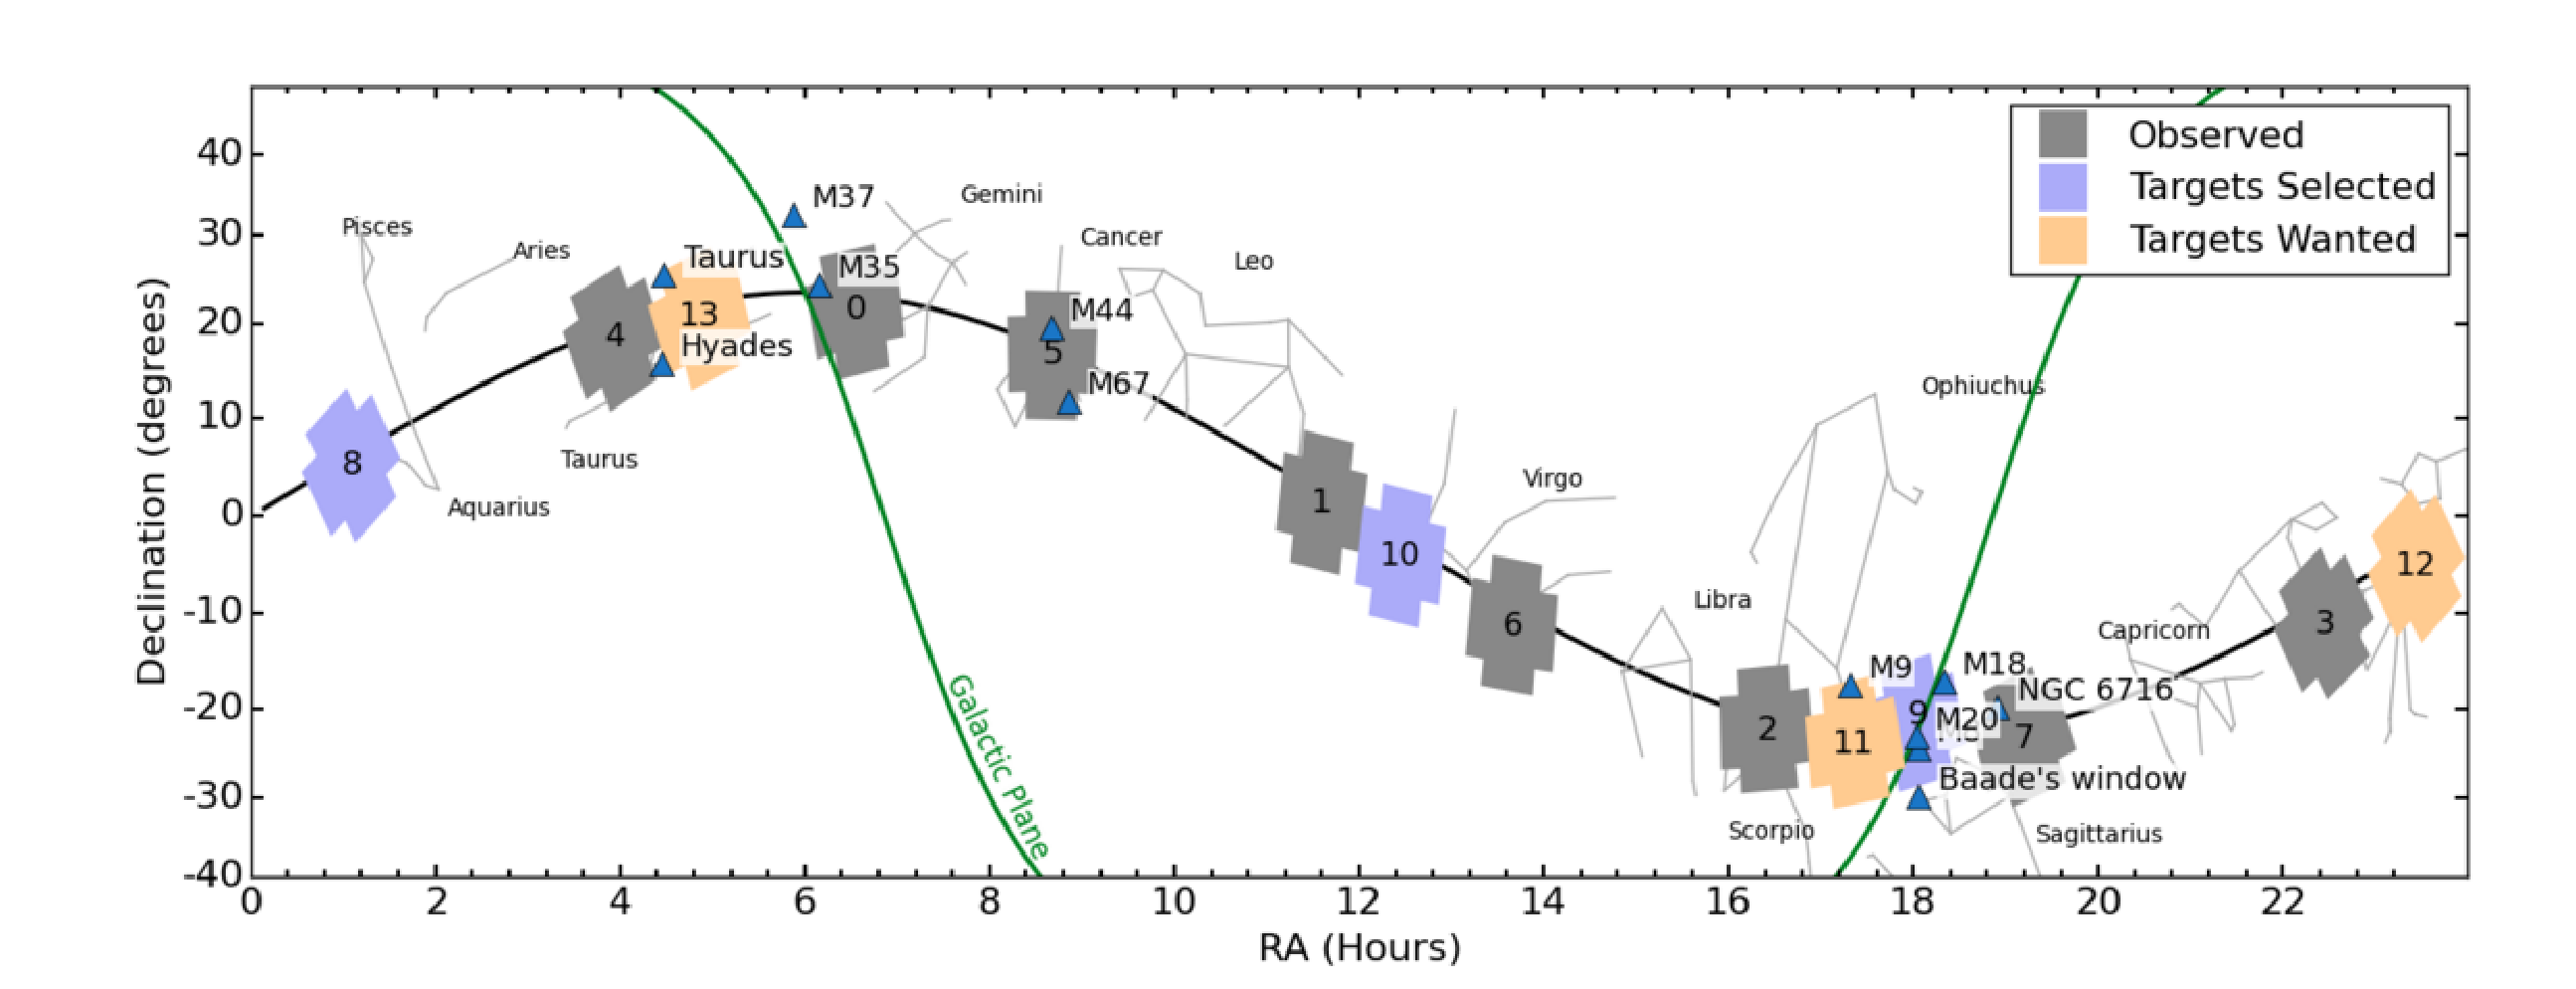
\includegraphics[width=6in, clip=true]{figures/Current_K2_fields.pdf}
\caption[Current \ktwo\ fields]{\ktwo's fields. Fields 1-9 have already been
observed and field 9 is being observed at the time this thesis is handed in.
Targets have been fixed for purple fields and proposals are currently being
solicited for yellow fields.}
\label{fig:current_fields}
\end{center}
\end{figure}

\begin{figure}[p]
\begin{center}
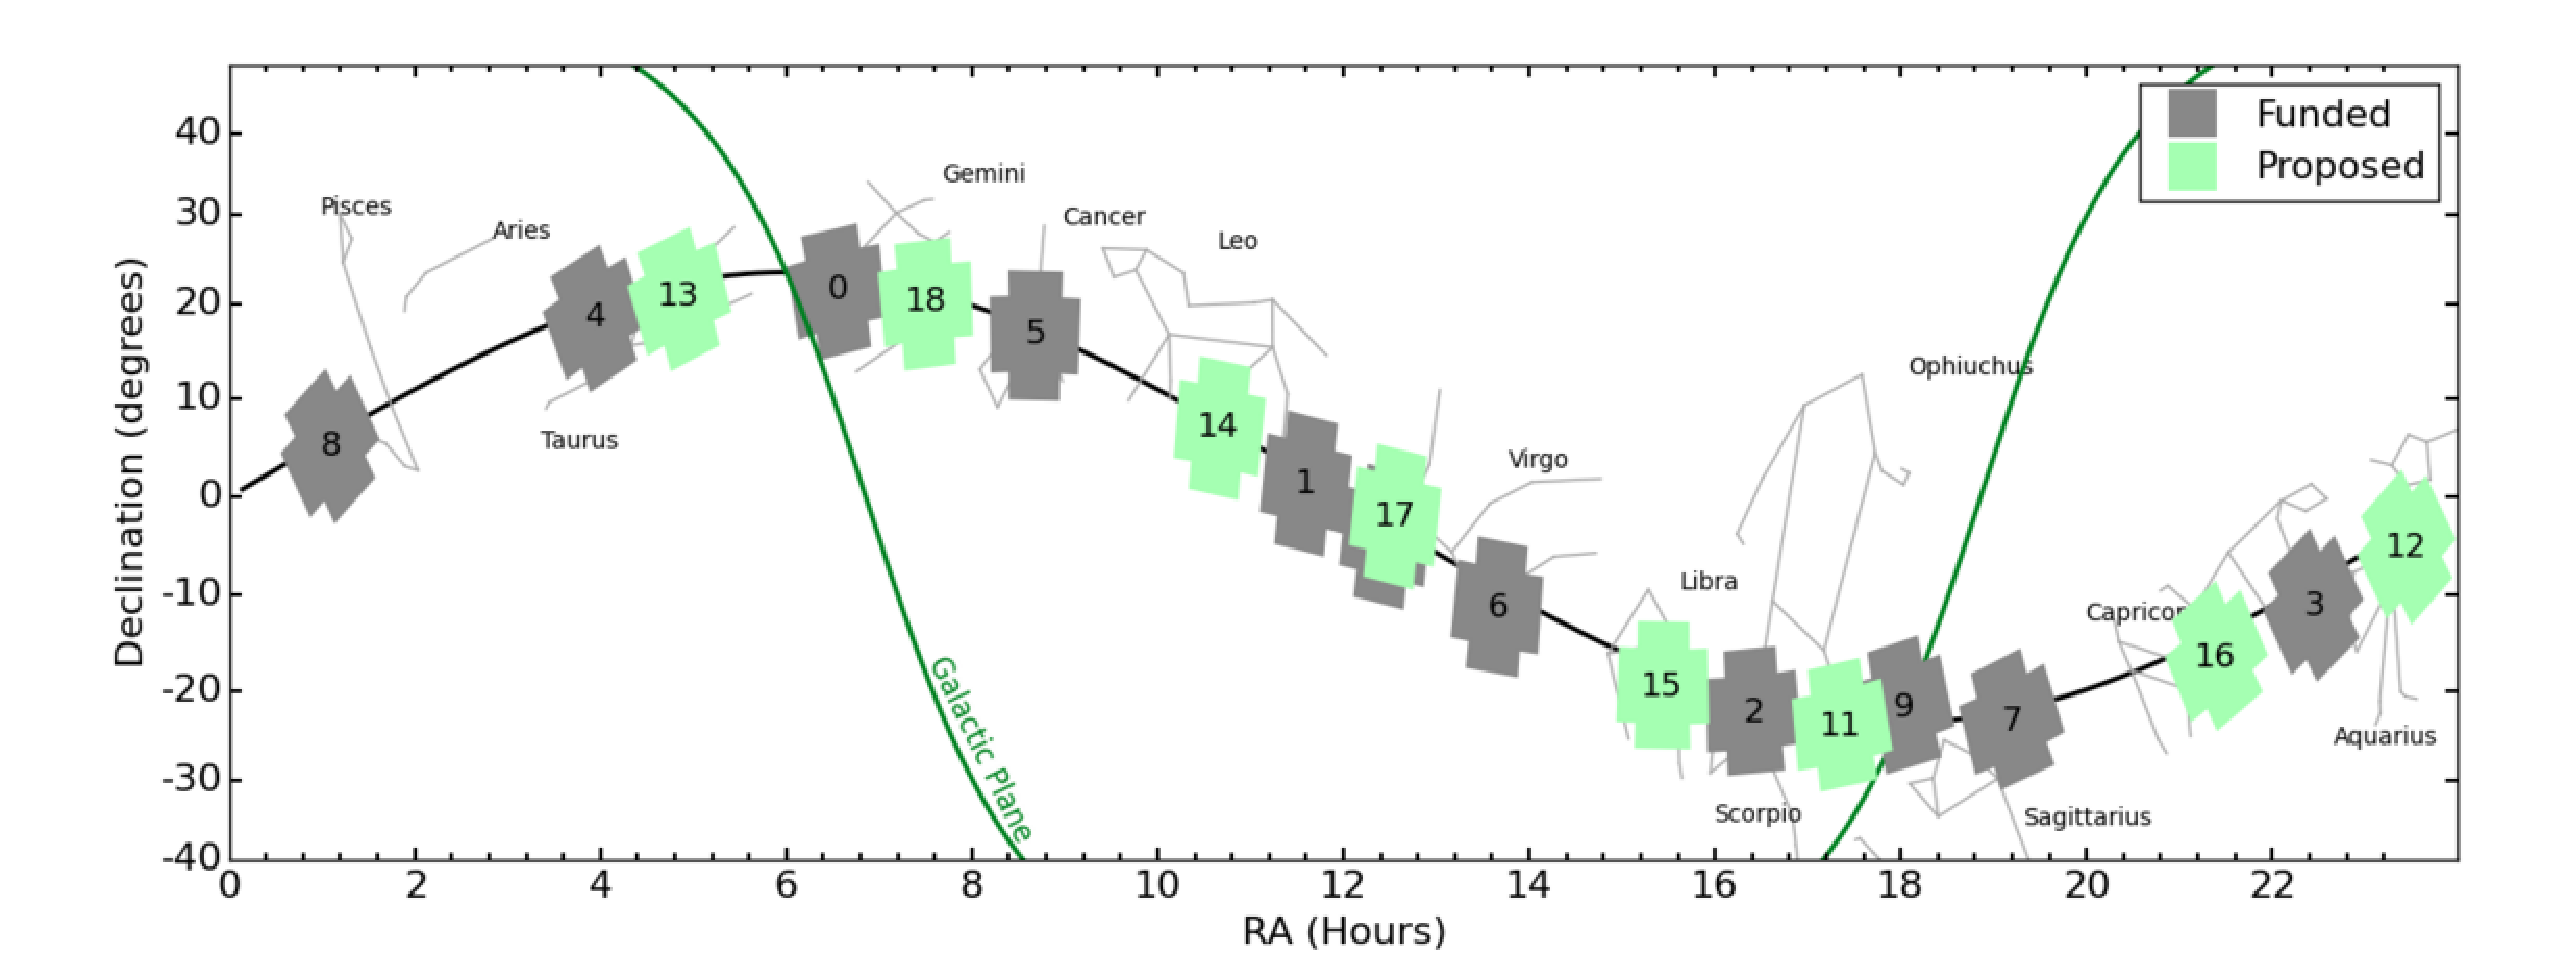
\includegraphics[width=6in, clip=true]{figures/Future_K2_fields.pdf}
\caption[Future \ktwo\ fields]{\ktwo's current and future fields. These green
fields are those proposed if an extended \ktwo\ mission is funded.}
\label{fig:future_fields}
\end{center}
\end{figure}

Not only is the spacecraft continuing its search for exoplanets \citep[and has
already discovered many, \eg][]{Vanderburg2015, Crossfield2015,
Foreman-Mackey2015, Montet2015, Becker2015, Vanderburg2016}, it will
provide time series of white dwarfs, active galactic nuclei, red giants, red
dwarfs, binary stars and other interesting astronomical objects.
Of course, with the reduced pointing position comes a new challenge for those
astronomers willing to get their hands dirty: systematic features in \ktwo\
light curves range from negliable for the brightest targets to dominant for
the faintest.
It is therefore necessary to employ heavy-duty `detrending' methods to
exploit \ktwo's rich data set.
This subject is covered in \textsection \ref{sec:detrending}

\section{Stellar dating methods}

\kepler's legacy is not limited to exoplanets---it has arguably advanced
stellar astronomy more than any other astronomical instrument ever created.
Amongst is several successes is the improvement of stellar dating methods, as
I explain below.

The hydrogen-burning era of a star's life is extremely stable.
This fact is unfortunate from a stellar chronologist's point of view as,
without an observable property that is a strong function of age, stellar age
precision will always be limited.
This is the main stumbling-block for stellar age inference: age precision is
restricted by the fundamental evolutionary time-scale of stars.
Despite this limitation however, there is still plenty of room for progress to
be made in understanding the evolution of the observable properties from both
empirical and theoretical standpoints, and in the precision with which we can
measure these properties.

Isochronal ages are notoriously difficult to infer because stars vary little
in brightness or temperature during their hydrogen-burning lifetimes.
Fitting stellar evolutionary models to these two observables usually produces
age estimates with uncertainties in the order of 50-150\%.
However, because cool stars spin down predictably over their main sequence
lifetime due to magnetic braking, their ages depend, to first order, only on
their masses and current rotation periods.
Photometric measurements of these two parameters can therefore be used to
infer an age.
This is the concept behind `gyrochronology'---inferring an age from a rotation
period---developed after observations of stars in clusters revealed a trend
for decreasing rotation period with time.
This method has never held as much promise as it does now, with a new glut of
stellar rotation periods available from a new generation of spacecraft
designed for high precision, high cadence photometry.
The main science goal of these missions is searching for exoplanets, but the
exoplanet gold-rush has lead to a new understanding of stars and stellar
variability.
The desire to develop a method of dating stars using only photometry is an
understandable one with the current availability of such large photometric
data sets.
However, as with any phenomenological investigation, inferences about the data
can only be made with models.
These models can be physical or empirical but whatever the origin of their
design, they must be calibrated using observations.
No age model can be developed in isolation from the observations---our
understanding of stars just isn't good enough.
So when a new dating method is developed, its efficacy relies on the existence
(and precision) of previous dating methods.
It is therefore important to understand the currently available dating
methods, their advantages and their limitations.
In what follows, I describe the main methods used today.

\subsection{Isochrone fitting}

As stars burn hydrogen they become hotter and more luminous, slowly moving
towards the top right of the Hertzprung-Russel Diagram (HRD), or
Colour-Magnitude Diagram (CMD).
As the hydrogen-burning process continues, helium `ash' is produced in the
core and energy production decreases.
The core slowly contracts over time and its temperature increases.
The increased temperature enhances energy production, and the result is that
stars burn hotter and more brightly over time.
If you can infer a star's absolute magnitude and effective temperature, or
measure its colour, and you have an idea of its composition and evolutionary
stage, you can place it on an HRD or CMD and infer its age.

In practice, it is not usually possible to feed luminosity, temperature,
metallicity and \logg\ into a stellar evolution model, crank the handle and
pull out an age.
Evaluating these models is expensive, so pre-calculated model grids are used.
In order to infer an age from the observations it is therefore necessary to
interpolate between the grid lines.
The Dartmouth \citep{dotter}, Yonsei-Yale \citep{spada} models are two of the
most commonly used sets of models.

An obvious limitation of the isochrone method is that the composition of the
star in question will affect its placement on a HRD or CMD: metal-rich stars
appear cooler and redder than metal-poor ones with the same mass and age.
% FIXME: why?
It is often difficult or impossible to obtain precise metallicities, helium
abundances and alpha-element fractions (all needed for precise isochrone
placement), as these measurements come from expensive, high-precision
spectroscopy.
% FIXME: how are these things actually extracted from spectra?
However, for an ensemble of coeval stars with identical compositions this
process becomes much easier: not only are there more opportunities to measure
stellar compositions, providing a $\sqrt N$ reduction in measurement
uncertainty, a group of stars with the same age and composition but different
masses will reveal the shape of the best-fitting isochrone on the CMD\@.
In addition, the position of the MS turn-off further improves age precision.
Since MS lifetime is strongly dependent on mass, at any given age the most
massive stars in a cluster will have turned off the MS.
Inferring the mass at which this happens in a cluster provides a very precise
age estimate.
% FIXME: what is the minimum age at which you can do this?
For these reasons, many open clusters have very precise ages.
Together with the Sun they are the most precisely dated of all astronomical
objects and provide the benchmarks from which all other dating methods are
calibrated.

% For example Pleiades (0.55 Gyr), Hyades (0.625 Gyr), Praesepe (0.588 Gyr), and
% Coma Berenices (0.5 Gyr).
% Download isochrones and estimate the ages of some KOIs.

\subsection{Asteroseismology}

After exoplanet search, arguably the second most important branch of \kepler's
legacy is asteroseismology; the study of stellar pulsations.
% QUESTION: difference between solar and classical pulsations?
% ANSWER: Solar are small enough that you can maintain certain approximations.
Sound waves ripple through the deep interiors of stars.
The frequencies of these waves can reveal internal structure, even localising
the hydrogen burning regions in stellar cores.
Asteroseismology is a powerful tool in the stellar dating arsenal.
Whilst asteroseismology is not the central topic of my thesis, it features at
some level in almost every chapter, so I have covered the basic principles in
what follows.

Acoustic oscillations in the Sun are generated by turbulent convection near
the surface.
The movement of ionized gas stochastically excites the Sun's spherical
oscillation modes.
An analogy to this process is that of a bell in a room filled with air.
Air particles colliding with the surface of the bell cause it to vibrate at
all of its spherical harmonic frequencies.
There is no coherent driving force, rather the stochastic collisions of air
particles induce a continual ringing.
Similarly, the Sun is continually oscillating at a range of discrete
frequencies; those that correspond to its spherical harmonics.
A power spectrum of the Sun, taken from \citet{brown} is shown in figure
~\ref{fig:solar_spectrum}.
The comb-like, evenly spaced peaks in this power spectrum show Solar p-mode
oscillations.
The peak amplitudes are modulated by a Gaussian envelope and the mean of that
Gaussian, $\nu_{max}$ corresponds to a frequency of around 3000 \uHz, a period
of around five minutes.

\begin{figure}[p]
\begin{center}
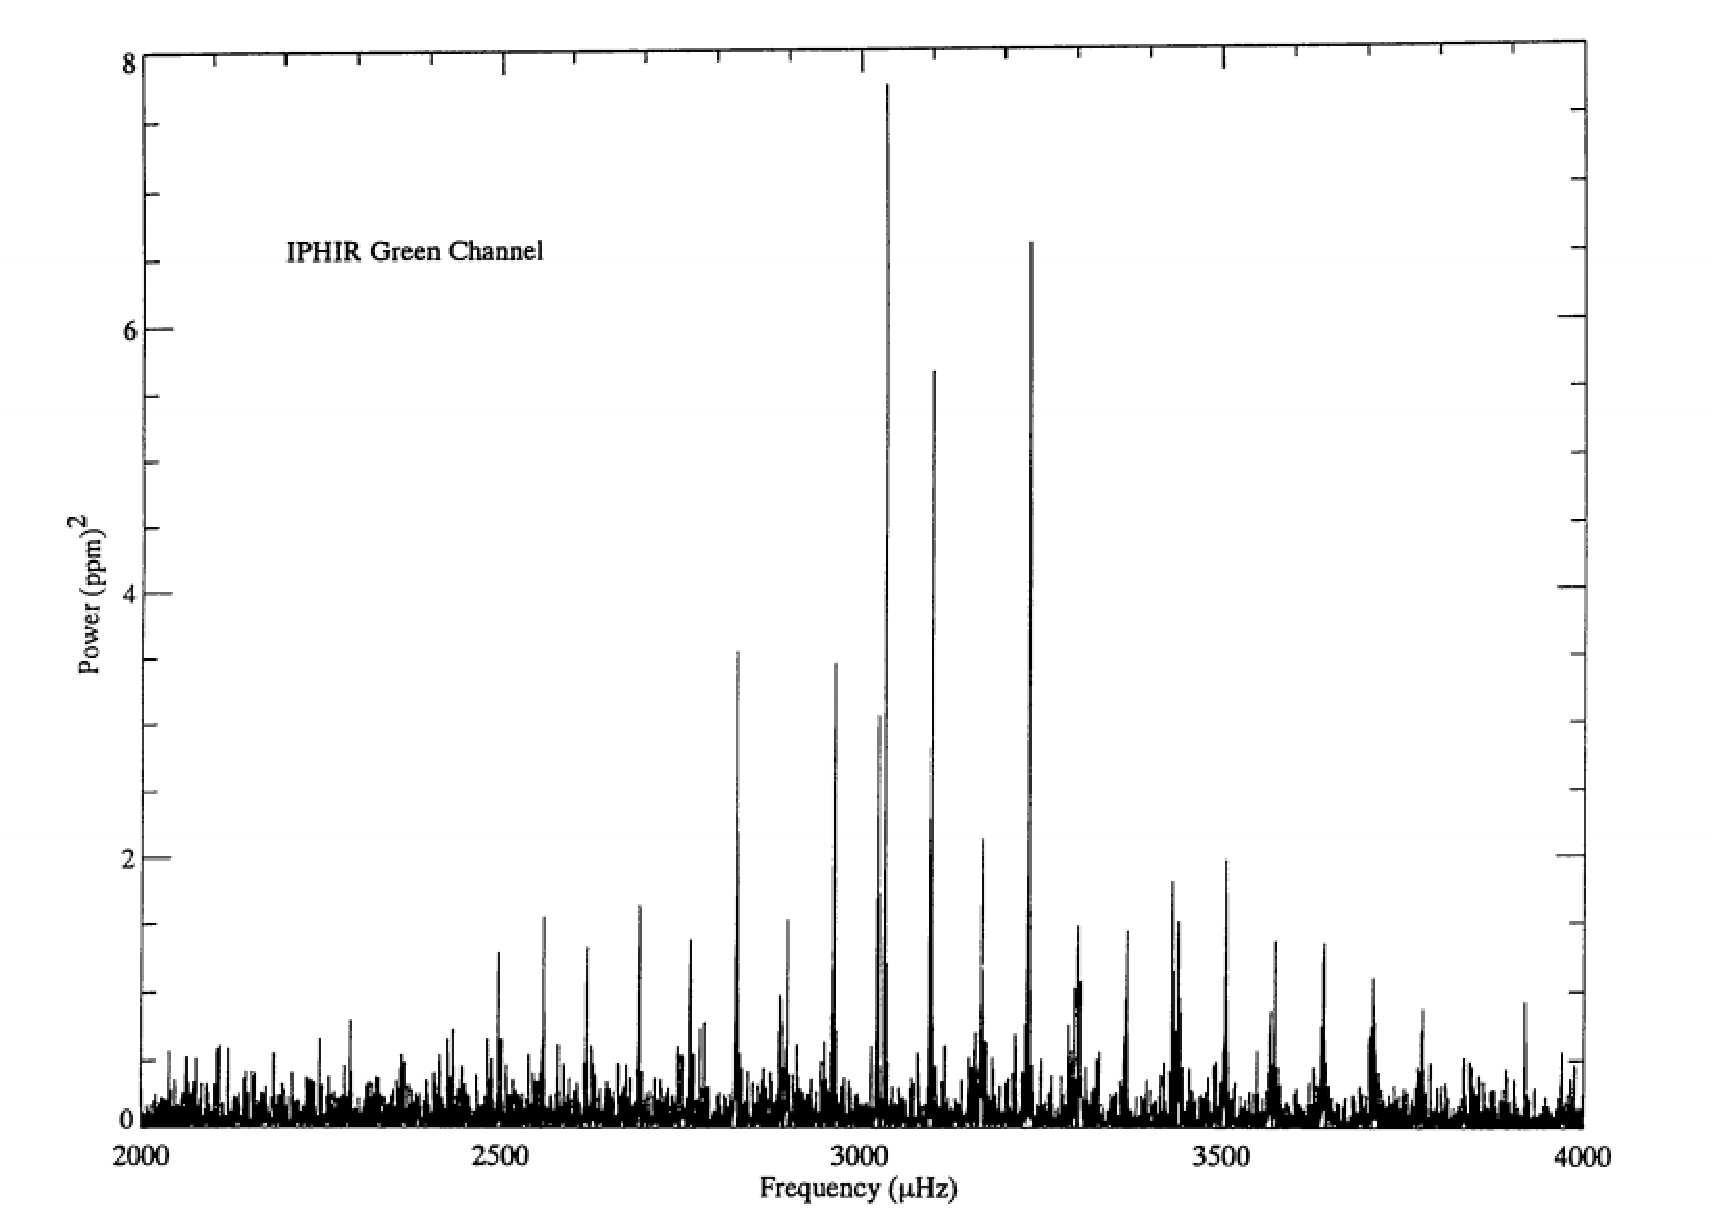
\includegraphics[width=6in, clip=true]{figures/solar_spectrum.pdf}
\caption[Solar power spectrum.]{A power spectrum of one month of
disk-integrated Solar photometry, taken from \citet{toutain}.
Solar p-modes are clearly visible in this figure.}
\label{fig:solar_spectrum}
\end{center}
\end{figure}

Many properties of the Sun have been measured using asteroseismic pulsations,
for example the variation in radial pressure, the rate of differential
rotation, the depth and fraction of helium in its convective zone and even the
structure of active regions below the Solar surface.
The Sun is an exquisite example of a pulsating star, having tens of millions
of detectable modes and mode lifetimes that are several thousand times longer
than the periods of the oscillations.
Its proximity, which provides both enormous signal-to-noise and allows us to
resolve the surface, make it a paragon of seismology.

Three types of oscillations are detectable in the Sun: pressure, or p-modes,
surface, s-modes and gravity, g-modes.
Pressure provides the restoring force for p-mode oscillations, and these are
effectively sound waves.
Surface modes are, as the name suggests, waves on the surface of the star.
% Since it is only possible to detect s-mode waves if the stellar surface is
% resolvable, this type of wave has only been seen in our Sun.
G-modes are excited by buoyant gas in the radiative zone and the restoring
force is gravity, hence the name.
These waves rapidly evanesce in stellar convective zones and therefore
appear at very low amplitudes at the surface of Sun-like stars.
For the work in this thesis I am concerned only with p-mode observations, as
these waves reveal the internal structure of a star which varies as a function
of mass, radius and age.

The frequency of a p-mode wave is proportional to the sound-speed of the gas
along its path through the stellar interior.
Time-dependent spatial perturbations to a star's equilibrium state can be
written as a product of a term that depends on stellar radius and a spherical
harmonic (assuming that a star can be approximated as a sphere) as follows
\citep{brown},
\begin{equation}
    \xi_{nlm}(r, \theta, \phi, t) = \xi_{nl}(r)Y_l^m(\theta, \
    \phi)e^{-i\omega_{nlm}t}.
\end{equation}
$\xi$ is a spatial perturbation, associated with a mode, $r, \theta, \phi,
\omega$ and $t$ are the radial coordinate, colatitude, longitude angular
frequency\footnote{The convention in asteroseismology is to report circular
frequencies, $\nu_{nlm} = \omega_{nlm}/2$.} and time, respectively.
$n$ is the radial order, defined as the number of nodes between the star's
centre and surface and $l$ is the angular degree, the product of the stellar
radius and the total horizontal wavenumber of the mode.
For example, a star oscillating with an $l = 10$ mode will have a standing
wave with 10 nodes along a line around the equator.
Finally, $m$ is the azimuthal order; the projection of $l$ onto the horizontal
wavenumber of mode and must be less than or equal to $l$.
A star with an $m = 5$ mode will have a standing wave with 5 nodes along a
line connecting its poles.
The relation between $\omega$ and $n$ and $l$ is complicated and depends on the
structure of the star.
Oscillations with different values of $l$ penetrate to different depths in the
star.
$l = 0$ waves travel through the centre and waves with increasing $l$ skirt
the central region by a larger and larger distance.
For this reason, modes with different $l$ provide information about the sound
speed gradient in the stellar interior.
The `small frequency separation', $\delta_{n,l} = \nu_{n+1, l} - \nu_{n, l+2}$
is often used to parameterise the variation in frequency with stellar radius
via \citep{brown}
\begin{equation}
    \delta_{n,l} = \Delta\nu_0\frac{(l + 1)}{2\pi^2\nu_{nl}}\int_0^{R_\star}
    \frac{dc}{dr}\frac{dr}{r}.
\end{equation}
Since nuclear-burning material in the core changes its molecular weight as the
star evolves, the sound-speed gradient is time-dependent and the small
separation therefore contains information about the age of the star.

There is no simple harmonic relation between the frequencies of modes with
adjacent mode number \citep{brown}.
% check this!
However, in the limit where $n \gg l$, mode frequency can be approximated as
\begin{equation}
    \nu_{nl} = \Delta\nu_0\left(n + \frac{l}{2} + \epsilon \right) - \
    \frac{AL^2 - \eta}{(n + l/2 + \eta)},
\end{equation}
where parameters $\Delta\nu_0$, $A$, $\epsilon$ and $\eta$ depend on the
structure of the star and $L^2 = l(l+1)$.
$\Delta\nu_0$ is the `large frequency separation' which, together with the
peak frequency of the Gaussian envelope that modulates the amplitudes of the
oscillation modes, $\nu_{max}$, makes up the two fundamental asteroseismic
observables.
It is related to the sound travel time through the centre of the star:
\begin{equation}
\Delta\nu_0 = \left(2\int_0^{R_\star}\frac{dr}{c}\right)^{-1},
\end{equation}
where $c$ is the local sound speed and $R_\star$ is the stellar radius.
This travel time is related to the mean density of the star via,
\begin{equation}
\Delta\nu_0 \cong 135\left(\frac{M_\star}{R_\star^3}\right)^{1/2}\mu Hz,
\end{equation}
where $M_\star$ and $R_\star$ are the stellar mass and radius in Solar units
\citep{cox, brown}.

Today, p-modes have been detected in hundreds of Sun-like stars, however it
was not until the late 1990s that the first conclusive detection was made in
a star other than our Sun.
The reason for this is simply that p-mode perturbations are extremely
small---these changes are around 10 cms$^{-1}$ in velocity and 3$\mu$mag in
brightness for typical oscillation modes in the Sun \citep{brown2000}.
Asteroseismic pulsations are usually detected in two different ways: by
searching for the subtle change in luminosity caused by the temperature
fluctuations of the stellar surface, or by measuring the changing radial
velocity of the surface.
A Fourier transform of these time series will reveal the presence of
oscillation modes, allowing for the modelling of the star's interior
structure.
The earliest p-modes detections were made using radial velocity data
\citep{kjeldsen2001} for stars $\eta$ {\bf Boo} \citep{kjeldsen1995}, {\bf
Procyon} \citep{barban1999, martic1999}, $\zeta$ {\bf Herculis}
\citep{martic2001}, $\alpha$ {\bf Cen A} \citep{kjeldsen1999} and $\beta$ {\bf
Hyi} \citep{bedding2001}.
Today, we have the advantage of space-based missions \kepler\ and \corot\
whose photometric precision provides sufficient signal-to-noise to detect
p-mode-induced luminosity variations.
These missions have provided fundamental parameters for hundreds of
oscillating giants, subgiants and Sun-like stars \citep[e.g.][]{michel2008,
bruntt2009, chaplin2014}.

% In the previous section I describe the relations between stellar p-mode
% oscillation frequencies and the physical parameters of a star.
% In this section I will describe the application of asteroseismology: how
% exactly does one infer fundamental stellar parameters from a light curve?
% My thesis work focuses on \kepler\ data, so this discussion will be directly
% related to \kepler\ data, but the same principles apply to other photometric
% time series.

The frequencies of astrophysical phenomena that are accessible in \kepler\
light curves are limited by two things: the overall duration of observations
and the time sampling.
The duration of observations, \ie\ the length of the \kepler\ mission sets the
minimum resolvable frequency and the time sampling sets the Nyquist frequency:
the high frequency limit.
For FGK dwarfs, the Nyquist frequency of long cadence observations ($\sim 283
\mu$Hz) is too low: these stars oscillate at around 3000 \uHz.
For this reason, \kepler\ operates in two observing modes: long and short
cadence \citep[][]{smith2012, stumpe2012}.
Long cadence observations are taken every approximately 30 minutes and short
cadence every minute ($\nu_{Nyquist} \sim 8333$\uHz).
Around 500 stars were observed in short cadence mode and the fundamental
parameters of these stars are presented in \citet{Chaplin2014}.

There are different approaches to inferring ages from \kepler\ light curves,
depending on the S/N of pulsations.
In the high S/N cases it may be possible to detect oscillation frequencies of
individual modes \citep[\eg][]{Lebreton2014, Metcalfe2010, Silva-aguirre2013}.
however for the majority of short cadence targets, only the
mean large frequency separation, $\Delta\nu$ and frequency of maximum power,
$\nu_{max}$ can be measured.
Bulk physical properties of stars can be inferred from these two parameters
via the scaling relations:
\begin{equation}
    \frac{M}{M_\odot} = \left(\frac{\nu_{max}}{\nu_{max,\odot}}\right)^3
    \left(\frac{\Delta\nu}{\Delta\nu_\odot}\right)^{-4}
    \left(\frac{T_{\mathrm{eff}}}{T_{\mathrm{eff},\odot}}\right)^{3/2}
\end{equation}
\begin{equation}
    \frac{R}{R_\odot} = \left(\frac{\nu_{max}}{\nu_{max,\odot}}\right)
    \left(\frac{\Delta\nu}{\Delta\nu_\odot}\right)^{-2}
    \left(\frac{T_{\mathrm{eff}}}{T_{\mathrm{eff},\odot}}\right)^{1/2}.
\end{equation}
Ages are then inferred by comparing these quantities to those predicted by
model grids (spectroscopic estimates of \teff and \feh are also required).
Ages inferred using \dnu and \numax typically have relatively large
uncertainties, in the order of 15-40\% \citep{Silva-aguirre2015a}.

In high S/N cases, ages are inferred by adjusting the parameters of stellar
interior models \citep[\eg][]{Kjeldsen2008} until the observed frequencies, or
combinations of them are reproduced.
Two of the most sophisticated codes used for age analysis are the BAyesian
STellar Algorithm \citep[BASTA][]{Silva-aguirre2015} and the Bellaterra
Stellar Properties Pipeline \citep{Serenelli2013}.
Uncertainties on ages inferred from high S/N light curves using this
`boutique' method of modelling individual frequencies are typically around
10-15\% \citep{Silva-aguirre2015a}.

Asteroseismology is a powerful dating method with the potential to yield
extremely precise stellar ages.
However, the era of asteroseismology has only just arrived and this fledgling
field is still only applicable to a small number of extremely bright stars
observed by precise photometric space-missions.
Given the quantity of up-and-coming photometric space missions,
asteroseismology will continue to provide precise stellar parameters for
decades to come.
However, accurate and precise asteroseismic ages demand high-precision
photometry of bright (brighter than around 12th magnitude) stars.
Even with \kepler\ and \corot, this only amounts to around one hundred MS
stars with asteroseismic ages available today.
It is therefore essential that alternative dating methods, which can be
applicable to a much larger sample of stars are developed.
Age-rotation relations, for example.

\subsection{Age-rotation relations}

Asteroseismology is revolutionising stellar astronomy and, perhaps, stellar
ages in particular (partly because the bar is so low to begin with).
However, the quantity of ultra-precise, short cadence light curves limited and
it is still a `boutique' method, applied to hand-picked, bright, text-book
Solar-like oscillators.
In order to produce a catalogue of stellar ages large enough to be useful for
stellar population studies, we need a method that can be applied to thousands
of stars.
Such a method should require inexpensive observables, be computationally cheap
and be easily automated.
Gyrochronology fulfills these criteria and in what follows I describe the
physics behind it.

\citet{Skumanich1972} compiled data that provided one of the first indications
that stellar rotation periods decay over time.
They demonstrated that rotation period, lithium abundance and chromospheric
activity decay was proportional to the square-root of age.
In figure \ref{fig:skumanich}, equatorial rotational velocity\footnote{ Only
the equatorial velocities of the G stars in the two clusters are indicated.}
versus time (triangles) is plotted on the same axes as lithium abundance
(crosses) and Ca$^+$ emission (circles) for the Hyades and Pleiades clusters,
as well as the Sun.
The Sun is the far right point for each age indicator.
Ursa Major stars are included on the Ca$^+$ emission scale.
Lithium abundance and Ca$^+$ emission were previously known age indicators and
this work demonstrated that rotation period was also related to age.
\begin{figure}
\begin{center}
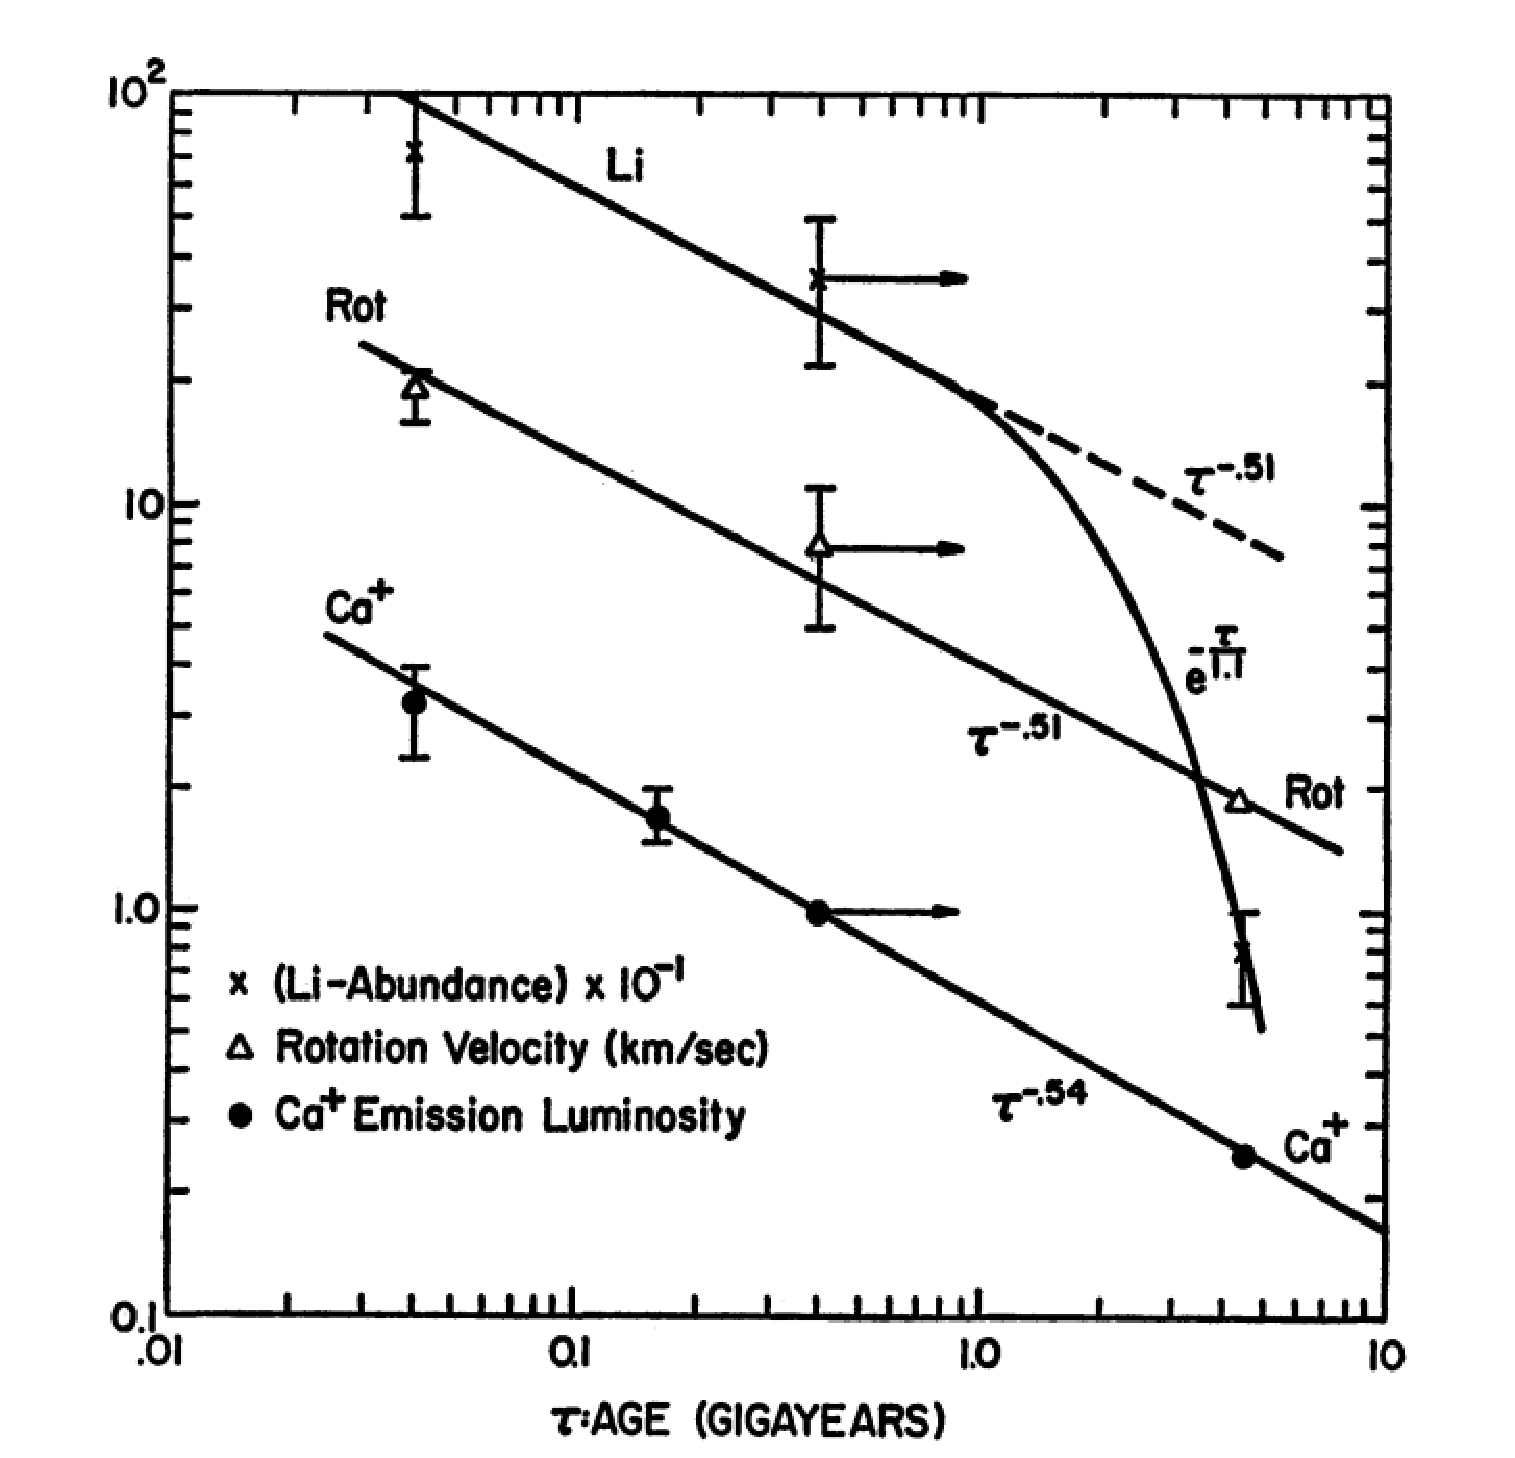
\includegraphics[width=3in, clip=true]{figures/skumanich.pdf}
\caption[\citet{skumanich1972} results: early evidence for magnetic braking]
{Figure from \citet{skumanich1972}. Rotation periods for the G stars in the
Hyades and Pleiades and the Sun are plotted.}
\label{fig:skumanich}
\end{center}
\end{figure}

% The rotation periods of cluster stars were investigated in several studies
% \citep[\eg][]{Stauffer1987}.
% The physical mechanism behind the coupling of stellar winds to the magnetic
% dynamo was explored by \citet{Weber1967, Mestel1984}.
% This process was later applied to evolving stars by \citet{Kawaler1988}.

Today, we know that angular momentum loss is caused by a magnetised stellar
wind \citep{Schatzman1962, Weber1967, Mestel1984}.
The stellar wind is composed of charged ions that stream away from the stellar
surface.
Each of these ions carries mass, charge and angular momentum as it travels
away from the star.
The angular momentum carried by these particles is lost from the system, not
at the surface, but at the point where they no longer co-rotate with the star.
Stellar magnetic fields force the particles in the stellar wind them to rotate
with the same angular velocity as the surface out to the Alfv{\'e}n radius.
The Alfv{\'e}n radius is the point at which a particle experiences equal force
from the magnetic field and the pressure produced by surrounding particles.
Once beyond the Alfv{\'e}n radius, the particles' angular momentum is lost
from the star.
This is dominant mechanism by which the rotation periods of stars decay during
their stint on the MS.
The stellar wind also carries mass away from the star, and the internal
structure of the star changes due to core hydrogen burning which both change
the star's moment of inertia, however these are secondary effects.

The motion of turbulent plasma in the outer layers of low-mass stars drives
the production of a magnetic field \citep[][]{Schatzman1962}.
% FIXME: how does rotation drive the dynamo?
Dynamo theory predicts that this field is then amplified by rotation and
differential rotation \citep[\eg][]{Parker1970}.
Convective turbulence, combined with stellar rotation produces the large-scale
magnetic fields that lock the stellar wind to the star
\citep[\eg][]{Charbonneau2010}.
Rotation period influences magnetic field strength: more rapid rotators have
stronger magnetic fields.
% FIXME: CITATION
The relation between angular momentum loss rate and angular velocity is a
power-law, where the exponent depends on the magnetic field geometry
\citet{Mestel1984, Kawaler1988}.
Magnetic field strength controls the rate of angular momentum loss: a stronger
magnetic field leads to a larger Alfv{\'e}n radius which increases the angular
momentum lost per unit time.
% There is a saturation point however, angular momentum loss rate only increases
% with magnetic field strength up to a point \citet{Chaboyer1995, Sills2000}.
For this reason the rate of angular momentum loss is not constant: as a star
loses angular momentum its rotation period decays as does its magnetic field
strength, so the rate of angular momentum loss decreases.
The effect of this process is to force stellar rotation periods to converge.
% \citet{Reiners2012} showed that angular momentum evolution is a function of
Rapid rotators have a greater angular momentum loss rate than slower rotators.
Their rotation periods therefore decay more rapidly than slow rotators and,
after a few hundred million years low mass stars appear to rotate at a rate
that depends, to first order, only on their age and mass.
This convergence happens more quickly for early-type stars than late-type.
Whilst FGK stars may have converged by 500 million years, \citep{Radick1987,
Irwin2009} late M dwarfs may not converge within a Hubble time.

Since the magnetic dynamo is believed to be generated in the convective zone,
stars with a thin convective layer have a weaker magnetic field.
For this reason they lose angular momentum more slowly.
Angular momentum loss rate therefore varies as a function of stellar mass and
fully radiative stars do not spin down appreciably over their MS lifetime
\citet{Noyes1984_2}.
The rotational evolution of fully stars convective is still unknown, however
it is an active field of interest \citep[\eg][]{Mcquillan2013, Newton2015}.

\citet{Barnes2003} compiled rotation period measurements from members of
several young clusters, plus the Mt. Wilson stars.
% (CITATION)
When the rotation periods of this sample were plotted against B-V colour,
\citet{Barnes2003} noticed that there were two morphological features of the
data (see their figure 2).
In each cluster there was a sequence of stars falling neatly on the predicted
relation between rotation period and mass (called interface, or `I' stars),
but there was also a group of rapid rotators (called convective, `C' stars).
The C sequence was most obvious in the younger clusters and less so in the
older.
\citet{Barnes2003} attributed this behaviour to an evolving magnetic dynamo,
produced by the still evolving internal structure of the young stars, and
postulated that stars transition rapidly from C to I.
In this work I will only address stars that have already (in theory) already
transitioned from the C sequence to the I sequence as they are older than the
Hyades which is the last cluster to show this behaviour.

\citet{Irwin2009} compiled rotation period measurements for stars in open
clusters with masses $< 1.2 M_\odot$, shown in figure \ref{fig:irwin}.
These data show the enormous spread in rotation periods for the youngest
clusters (top left), contrasted with the extremely well-defined rotational
sequence in the Hyades (second panel from the bottom on the right).
The currently accepted view is that after the age of the Hyades, stellar
rotation periods lie on this converged sequence.
In this thesis I will only discuss stars older than around the age of the
Hyades.
\begin{figure}[p]
\begin{center}
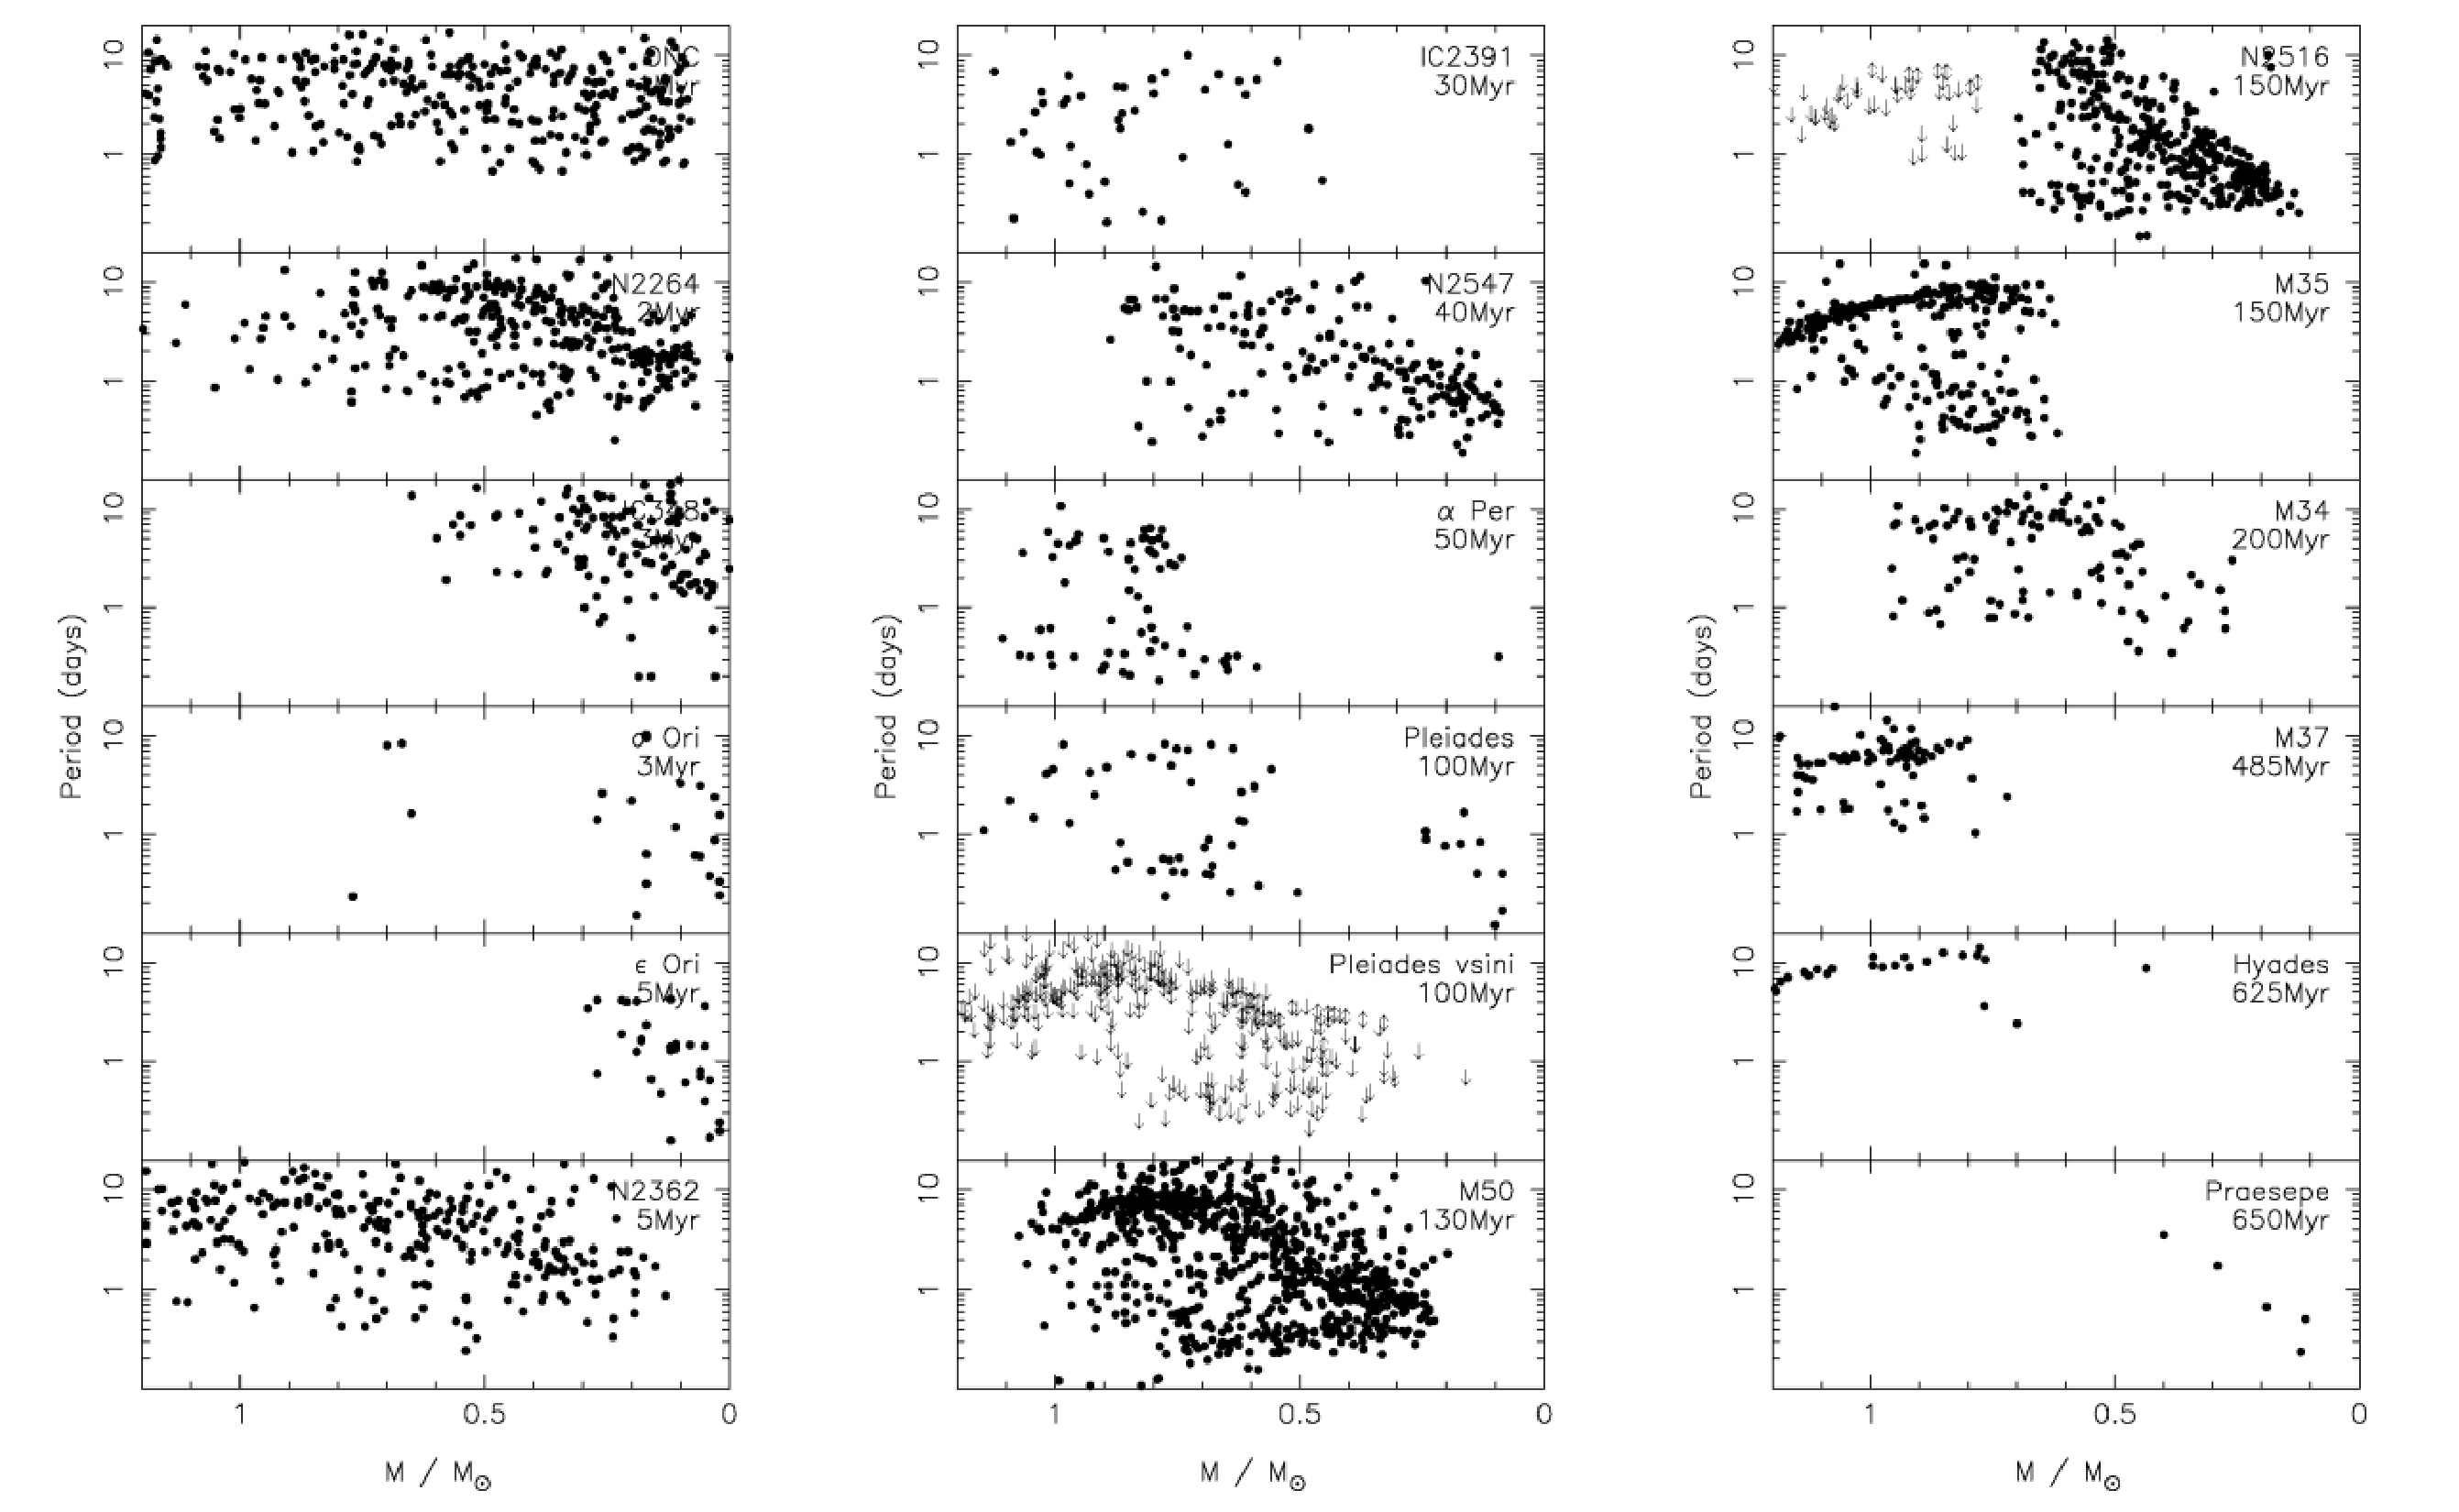
\includegraphics[width=4in, clip=true]{figures/irwin.pdf}
\caption[Cluster rotation from \citet{Irwin2009}]
{Figure from \citet{Irwin2009}. A compilation of most of the available
rotation periods for stars in open clusters with $M < 1.2 M_\odot$ in 2009.
Clusters increase in age from the top left to the bottom right.}
\label{fig:solar_spectrum}
\end{center}
\end{figure}

The term `gyrochronology' was first coined by \citet{Barnes2003}.
Several gyrochronology models have been developed by different groups since
then.
Some of these \citep[\eg][]{Kawaler1988, Collier-cameron1994, Reiners2012,
Epstein2014, VanSaders2014} use physical models of rotating stars with
magnetic fields, where the rate of angular momentum loss is related to the
rotation period and field strength, and evolve those stars forward in time.
Although these models are based on the physical processes at play, they must
still be calibrated using observations.
For example, the \citet{Kawaler1988} expression, assuming a linear dynamo is
\begin{equation}
\frac{dJ}{dt} = -K_w\Omega^3\left(\frac{R}{R_\odot}\right)^{0.5}
\left(\frac{M}{M_\odot}\right)^{-0.5},
\end{equation}
where $J$ is angular momentum, $R$ and $M$ are radius and mass respectively
and $K_w$ is a constant that must be calibrated so that the Sun has Solar
rotation at Solar age.
See \citet{Barnes2010b} for a discussion on the various adaptations of this
braking law, taken by different groups in order to reproduce observations of
young clusters.
\citet{Vansaders2014} use the following model to describe the rotation period
distribution of cool field stars:
\begin{equation}
\frac{dJ}{dt} = \left\{
                \begin{array}{ll}
                  f_K K_M \omega \left( \frac{\omega_{crit}}{\omega_\odot}
                  \right)^2, \omega_{crit} \leq \omega
                  \frac{\tau_{c}}{\tau_{c, \odot}} \\
                  f_K K_M \omega \left( \frac{\omega\tau_{c}}
                  {\omega_\odot\tau_{c, \odot}}
                  \right)^2, \omega_{crit} > \omega
                  \frac{\tau_{c}}{\tau_{c, \odot}}
                \end{array}
              \right.
\end{equation}
\label{eq:vansaders}
With
\begin{equation}
    \frac{K_M}{K_{M, \odot}} = c(\omega)\left(\frac{R}{R_\odot}^{3.1}\right)
    \left(\frac{M}{M_\odot}\right)^{-0.22}
    \left(\frac{L}{L_\odot}\right)^{0.56}
    \left(\frac{P_{phot}}{P_{phot, \odot}}\right)^{0.44},
\end{equation}
\label{eq:vansaders2}
where $f_K$ is a constant, scaled to produce solar rotation at solar age for
the Sun and $P_{phot}$ is the pressure at the photosphere.

An alternative approach is an entirely empirical one where simple functional
forms are fit to the observations \citep[\eg][]{Barnes2007, Mamajek2008,
Meibom2010}.
\citet{Barnes2003} proposed the following functional form for the relation
between period, colour and age, \begin{equation} \label{eq:Barnes2007_2} P =
A^n \times a(B-V-c)^b, \end{equation} where $P$ is rotation period (in days),
$A$ is age (in Myr), $B$ and $V$ are B and V band magnitudes respectively and
$a$, $b$, $c$ and $n$ are dimensionless free parameters.
\citet{Barnes2007} used rotation periods for stars in open clusters ranging in
age from 30-600 Myr to calibrate this relation.
This same functional form was used by \citet{Mamajek2008} and
\citet{Meibom2010} who also used young clusters to recalibrate the
gyrochronology model.

\citet{Barnes2010b} present a hybrid part theoretical, part empirical
gyrochronology relation,
\begin{equation}
\frac{dP}{dt} = \frac{\tau_c}{k_IP_{rot}},
\end{equation}
where $k_I$ is a dimensionless constant, calibrated with observations.
The convective overturn time, $\tau_c$ encodes the dependence on stellar mass.

\section{Other age diagnostics}

\subsection{Activity}
Stars are born very active and become more inactive over time.
As well as decaying over billions of years, activity also varies on year
timescales.
The most notable example is the Sun which has an 11 year cycle.
The activity cycle period, $P_{cyc}$ is related to rotation period, $P_{rot}$
via $P_{cyc} \approx (P_{rot}/\tau_c)^n$ where n $\approx$ 1.5 and $\tau_c$ is
the convective overturn time at the base of the convective zone
\citep{Noyes1984}.
$P_{rot}/\tau_c$ is known as the Rossby number, $Ro$.
It is therefore dependent on spectral type and for this reason many people
argue that Rossby number is directly related to the surface magnetic field
strengh and a more natural quantity to correlate with age and activity than
rotation period \citep[\eg][]{Vansaders2015} \citep[although this view is not
universally held][]{Reiners2014}.
Although stellar activity originates from one mechanism only: magnetism,
it manifests in a variety of detectable ways, listed below.
\begin{itemize}
\item{Star spots.
Surface differential rotation, where the equator rotates at a different speed
to the poles (in the Sun it rotates faster), twists the magnetic flux into
tubes which emerge from the stellar surface.
The convection of material at the points where they emerge is inhibited and
these areas are cooler and darker as a result.
These cool, dark regions are called Sun spots on the Sun and star spots on the
surfaces of other stars.
Because these regions are darker, the integrated, optical flux emitted by a
star when there are more spots on the surface is decreased.
These decreases in brightness are detectable on the time scale of the stellar
rotation period, where spots rotate into and out of view, and on longer
timescales---the overall activity cycle.
The Sun has an activity cycle that lasts 11 years.
During periods of low activity the Solar surface has few star spots and this
number increases up to hundred of spots during the Solar maximum.}
\item{Chromospheric activity.
Magnetic activity in stellar chromospheres produces emission in the cores of
singly ionised calcium H (3969.5$\AA$) and K\footnote{The H and K letters
indicate the Fraunhofer designation.
Fraunhofer assigned letters to the absorption lines he detected in the Solar
spectrum.} (3933.7$\AA$) lines.
This emission reversal is produced by the excitation of Ca$^+$ electrons to a
higher energy level via magnetic heating.
Just as with rotation period, chromospheric activity decreases with time and
the two properties are related \citep[\eg][]{Kraft1967, Noyes1984b}.
Relations between age and chromospheric activity have, just as with rotation
period, been calibrated \citep[\eg][]{Soderblom1991, Donahue1993,
Lachaume1999, Mamajek2008}.
Chromospheric activity is usually quantified via the R$\prime_{HK}$ index,
defined as the flux excess in the lines, normalised to the bolometric flux.
The drawback of using chromospheric activity indices are similar to the
drawbacks of gyrochronology: the data are sparse and particularly so at late
ages and low masses.
Crucially though, measurements of Ca II H \& K emission are difficult to
obtain since high-resolution spectra are required.
}
\item{UV and X-ray flux.}
Magnetic heating in the corona and chromosphere excites photons to high
energies, producing substantial UV and X-ray fluxes
\citep[\eg][]{Pallavicini1981}.
Since M dwarfs have large convective zones, some even being fully convective,
they are highly active.
Their UV flux is significant which is currently causing ripples in the
exoplanet community.
M dwarfs with transiting exoplanets are premium targets for follow-up with the
James Webb Space Telescope (JWST) since their petite size relative to their
Earth-radius planets provides deep transits.
The large signal-to-noise ratios of these deep transits will allow JWST to
search for biomarkers in the atmospheres of these planets.
However, since M dwarfs are more active than G dwarfs, and their habitable
zones are closer in, any potential life on an Earth-twins may have been
obliterated by the extreme UV flux.
\item{Flare rate.
Convective turbulence in low-mass stars generates magnetic flux tubes.
Differential rotation then causes these flux tubes to twist around each other,
becoming entangled.
Magnetic reconnection causes the acceleration of particles and a huge amount
of energy is released into the Inter-Stellar Medium (ISM).
The flare rate is related to the mean flare energy via a power law
\citep{Davenport2015, Hawley2014} and both of these properties are related to
the strength of the stellar magnetic field.
Flares occur extremely often in M dwarfs, the most magnetically active stars,
with energies ranging from $\sim e^{29} - e^{33}$ ergs and durations ranging
from a few to a hundred minutes \citep{Hawley2014}.
% FIXME: what drives differential rotation?
}
\end{itemize}

\subsection{Lithium depletion boundary}
The Lithium Depletion Boundary (LDB) can be used as an age diagnostic for
young, low mass ($<1M_\odot$) stars.
As these young stars contract on the Pre-Main Sequence (PMS) their core
temperature increases.
When it reaches $\sim2.5\times10^6$ K, lithium is destroyed via $^7$Li$(p,
\alpha)^4$He and $^6$Li$(p, \alpha)^3$He proton capture reactions
\citep[\eg][]{Bodenheimer1965}.
The time taken for a star to reach these temperatures depends on their mass.
The lowest mass PMS stars are fully convective, so the mixing timescale is
very short and lithium depletion takes place very rapidly.
For young stellar groups therefore, the mass at which the LDB (the boundary
stars that do and do not show lithium in their atmospheres) is located is a
very sensitive function of age \citep{Basri1996}.
LDB dating can be very precise \citep{Burke2004}, however it is only
applicable to young groups of stars (20 Myr < age < 200 Myr) since by this
time Lithium has disappeared from the atmospheres of all members, regardless
of their mass.

\subsection{Dynamics}
Stellar populations in the Milky Way galaxy can be localised into four groups:
the bulge, the thin disk, the thick disc and the halo.
Each of these stellar populations has a different distribution of stellar
ages.
The bulge is comprised of old stars.
It is characteristically red because the only remaining stars on the MS are
low-mass.
The thin disk is comprised of young stars.
This is the main star-forming part of the galaxy as the spiral arms, density
waves of molecular gas that readily collapses into protostars, reside in the
thin disk.
The orbits of thin disk stars get heated over time.
Close encounters with neighbouring stars boost their orbital energies and many
thin disc stars find themselves `kicked' out of the galactic plane into the
`thick disc'.
The thick disc is statistically older than the thin disc since the majority of
its residents have had time to experience one or more close encounters.
The halo is even older still: these stars have been displaced even further
from the thin disk in which they were born.
Scince the probability of experiencing a close encounter increases with time,
stars with higher proper motions are likely to be older \citep[see,
\eg][]{Shevelev1989, Nissen1991}.
However, although a rapidly moving star is likely to be older than a slowly
moving star, stellar-orbit heating is a stochastic process and therefore
cannot always be relied upon.

\section{Statistical methods}

A core part of this thesis is the statistical methods that are employed.
None of the methods used here are new in themselves, but many have not been
previously used on the sorts of problems that are presented here or in an
astronomical context.
I will now discuss them in the order in which they feature in the subsequent
chapters of this thesis.

\subsection{Multi-dimensional and unknown uncertainties: hierarchical
probabilistic modelling}
In some cases in astronomy, the only significant uncertainties are on
the dependent variable.
This is often the case with time-series or spectra and assuming that the
independent variable uncertainties are negligible is a reasonable assumption.
In a case where one wants to fit a model to data where the only significant
uncertainties lie in the $y$ direction, those uncertainties are Gaussian, the
measurements are independent and there is no correlated noise, it may be
appropriate to use the Gaussian likelihood function.
For example the likelihood of $y$-values, given some $x$-values, some model
parameters, $\mathbf{\theta}$ and some $y$-direction uncertainties, $\sigma$,
the likelihood can be written
\begin{equation}
    p(y|x, \sigma, \mathbf{\theta}) = \prod_{i=1}^N
    \frac{1}{\sqrt{2\pi\sigma_i^2}}
    \exp\left(-\frac{[y_i - \mu(x_i, \mathbf{\theta})]^2}{2\sigma_i^2}\right),
\end{equation}
where $\mu$ is the mean model.
It is often more practical to use the logarithm of this function,
\begin{equation}
    \ln\mathcal{L} =
    -\frac{1}{2} \sum_{i=1}^N \left[\frac{[y_i - \mu(x_i,
    \mathbf{\theta})]^2}{\sigma_i^2} +
    \ln\left(2\pi\sigma_i^2\right) \right],
\end{equation}
\label{eq:lnlike}
which is also known as $-\frac{1}{2}\chi^2$.

In many fitting-model-to-data problems in the astronomical literature,
a frequentist approach is taken and $\chi^2$ is minimised (which is the
equivalent of maximising the log-likelihood).
The probabilistic (Bayesian) approach however is to multiply this likelihood
by a prior to produce a posterior Probability Density Function (PDF).
\begin{equation}
Bayes rule
\end{equation}
The prior represents one's prior beliefs about the model parameters,
$\mathbf{\theta}$.
There is a wide range of literature available on the science behind choosing
priors which is beyond the scope of this thesis.
% CITATIONS

Returning to equation \ref{eq:lnlike}, it is trivial to modify this function
for the case where the $y$-direction uncertainties are unknown, or
under-(or over)-estimated.
In this case one could write
\begin{equation}
    \ln\mathcal{L} =
    -\frac{1}{2} \sum_{i=1}^N \left[\frac{[y_i - \mu(x_i,
    \mathbf{\theta})]^2}{\sigma_i^2 + s^2} +
    \ln\left(2\pi(\sigma_i^2 + s^2\right) \right],
\end{equation}
where $s^2$ is the additional variance needed to explain the scatter in the
data.

In chapter \ref{chapter:flicker} a modification to the above equation is used
to fit a line to data where the uncertainties are underestimated.
This is a hierarchical problem, since there are two parameters that describe
the model (a straight line), $\alpha$ and $\beta$, where $\mu = \alpha +
\beta x$ and a parameter describes the standard deviation of a Gaussian
spanning the mean model.
In other words, the `true' value of variable $y$---the value that would have
been measured if there were no observational uncertainties, $\bar{y}$ is drawn
from a Gaussian with mean, $\mu = \alpha + \beta \bar{x}$ and standard
deviation, $s$:
\begin{equation}
\bar{y} \sim \mathcal{N}(\alpha + \beta\bar{x}, s^2),
\end{equation}
and the {\it observations}, $y_{obs}$ are in turn drawn from Gaussians with
$\mu = \bar{y}$ and standard deviations described by the individual
observational uncertainties, $\sigma_{obs}$:
\begin{equation}
y_{obs} \sim \mathcal{N}(\bar{y}, \sigma_{obs}^2).
\end{equation}
Since it is the observations that are modelled, not the latent parameter,
$\bar{y}$, this is a hierarchical process.

Equation \ref{eq:lnlike} can also be modified for the simple case of fitting a
straight line to data, where the $y$-direction observational uncertainties are
unknown {\it and} the $x$-direction uncertainties are non-negligible.
Starting from equations 26, 29, 31 and 32 of \citet{Hogg2010},
$\mathbf{S_i}$ is the covariance tensor,
\begin{eqnarray}
    \mathbf{S_i} &\equiv& \left( \begin{array}{cc}
                    \sigma_{x}^2 & \sigma_{x,y} \\
                    \sigma_{x,y} & \sigma_{y}^2
\end{array}\right),
\end{eqnarray}
\label{eq:covariance_tensor}
$\mathbf{\hat{\nu}}$ is a unit vector orthogonal to the line with slope
$\alpha$,
\begin{equation}
    \mathbf{\hat{\nu}} = \frac{1}{\sqrt{1 + \alpha^2}} \left( \begin{array}{c}
                                                    -\alpha \\
                                                    1
    \end{array}\right),
\end{equation}
\label{eq:unit_vector}
the variance is given by,
\begin{equation}
    \Sigma_i^2 = \mathbf{\hat{\nu}}^T \mathbf{S_i} \mathbf{\hat{\nu}}
\end{equation}
\label{eq:variance}
and the log-likelihood can be written,
\begin{equation}
    \ln\mathcal{L} = - \frac{1}{2} \sum_{i=1}^N \left[
    \frac{\Delta_i^2}{\Sigma_i^2} + \ln|\mathbf{S_i}| \right].
\end{equation}
\label{eq:ndlnlike}
By modifying equation \ref{eq:covariance_tensor} to be
\begin{eqnarray}
    \mathbf{S_i} &=& \left( \begin{array}{cc}
                    \sigma_{x}^2 & 0 \\
                    0 & \sigma_{y}^2 + s^2
\end{array}\right),
\end{eqnarray}
\label{eq:covariance_tensor_mod}
since we assume that the covariance between $x$ and $y$ is negligible,
substituting \ref{eq:covariance_tensor_mod}, \ref{eq:unit_vector} \&
\ref{eq:variance} into \ref{eq:ndlnlike} gives
\begin{equation}
    \ln(\mathcal{L}) = -\frac{1}{2} \sum_{i=1}^N
    \left( \frac{\left[ y_i - (\alpha + \beta x_i) \right]^2}
    {\beta^2\sigma_{x, i} + \sigma_{y, i}^2 + s^2} + \ln[\sigma_{x,
    i}^2(\sigma_{y, i}^2 + s^2)]
    \right)
\end{equation}.
This is the equation used in chapter \ref{chapter:flicker} to perform such an
analysis with astrophysical data.

In cases with more complicated mean models, it is not so easy to arrive at an
analytic solution.
For example, a similar problem is approached in chapter \ref{chapter:gyro}.
Here, the extra variance parameter, $s$ is not used (although it should be
included in future analyses!), however the uncertainties in the $x$, $y$, and
this time $z$ too, directions are large.
The model is not a simple two-dimensional line as in the above case, it is the
three-dimensional gyrochronology equation \ref{eq:barnes} where $y$ is
rotation period, $x$ is age and $z$ is B-V colour.
In this case, an approximation must be made in order to take the uncertainties
on all dimensions into account.
This approximation is made via sampling and is described in chapter
\ref{chapter:gyro}.

\subsection{Methods for removing systematics}
\label{sec:detrending}

`Detrending' is a word that has been adopted by astronomers to mean removing
systematic trends caused by non-physical (\eg instrumental) variations in the
experiment conditions.
This process can be applied to any data set that contains correlated noise, be
it a time series, image or spectrum, however `detrending' usually pertains
specifically to time series analysis, and light curves in particular.
The detrending process involves the generation of some model of the systematic
features that can be generated and then subtracted from the light curve.
This implies that the contribution of systematics to the light curve are known
{\it a priori}.
Of course in reality, the contributions coming from the signal and the noise
can never be known completely, so must be approximated.
In some cases this approximation is close to the truth, or doesn't need to be
for the purposes of extracting science from the data (for example, if
instrumental systematics exist on very different timescales to the signal of
interest).
However, in many cases the noise model cannot be adequately approximated.
At best this leads to inaccurate inferences about the physical system being
studied and at worse it leads to false positive detections and false negative
non-detections.

In \textsection \ref{chapter:sip} I present a method for extracting periodic
signals from \ktwo\ light curves, without detrending.
In what follows I review a selection of detrending methods.

\kepler\ data is available to download at various stages of the reduction
process.
Target Pixel Files (TPFs), are arrays of the raw pixel fluxes, Simple Aperture
Photometry (SAP) light curves, are generated by combining pixel fluxes with
simple masks and Presearch Data Conditioned Maximum {\it a posteriori}
(PDC-MAP) light curves, a detrended data product.

The detrending process concerns removing as much of the noise as possible
whilst preserving the signal \citep{Smith2012, Stumpe2012}.
In reality no detrending process does this perfectly and most favour a
slightly more or less aggressive approach to removing systematics, depending
on the science goal.
Systematic features in \kepler\ light curves are generated by two main
sources: pointing variations and temperature variations, although pointing
variations are more serious for \ktwo\ light curves than \kepler\ light
curves.
Regardless of the source, either of these variations will effect stars that
lie close together on the CCD in similar ways.
The \kepler\ pipeline uses this fact to isolate physical signals from
instrumental: physical signals vary from star to star and intrumental signals
are present in nearby groups of light curves.
Stars that are nearby, intrinsically quiet, but display similar patterns in
variation are used to generate a set of Cotrending Basis Vectors (CBVs) via
Single Value Decomposition (SVD).
A detrending model, constructed from a linear combination of CBVs is then fit
to these stars and the distribution of the CBV weights are used to generate a
prior.
A systematics model is then fit to each individual light curve, where a
likelihood function is multiplied by the prior and the resulting maximum of
the posterior PDF is taken to be the best fit.
That systematics model is then subtracted from the data.

PDC-MAP light curves were designed to maximise exoplanet transit search
capability.
These signals are rarely longer than thirteen hours and have a characteristic
upside-down top-hat shape.
Stellar variability on the other hand is smoothly varying (similarly to
systematic features) with timescales ranging from around one day to several
years.
% PDC-MAP detrending does not preserve signals longer than $\sim$ 30 days.
% FIXME: find this CITATION

An alternative approach to PDC-MAP detrending, designed to preserve signals
from the stars as {\it well} as the planets is that of \citet{Roberts2013}.
They also fit a linear combination of CBVs to the data, however the main
differences in their approach are to impose a maximum entropy criterion:
trends in the most highly-weighted CBVs must be present in a large number of
light curves, and to remove high frequency noise from the systematics model
before detrending so as not to inject noise.
A comparison of the two detrending methods is presented in
\citet{Roberts2013}.

Once \kepler\ lost its third reaction wheel, pointing variations became much
more severe, systematic features rose in amplitude and more aggressive
detrending techniques became necessary.

\subsection{Rotation period inference}
% could move this to chapter 5

\subsubsection{ACF}
An AutoCorrelation Function (ACF) was first used to measure rotation periods
by \citet{Mcquillan2013} who developed the method specifically for \kepler\
data.

\subsubsection{Lomb-Scargle}
\subsubsection{Wavelets}
\subsubsection{Spectroscopy}

% \newcommand{\logg}{log \emph{g}}
\newcommand{\prot}{$P_{rot}~$}
\newcommand{\w}{\mathbf{w}}
\newcommand{\wh}{$\hat{\mathbf{w}}_n$}
\newcommand{\ah}{$\hat{A}_n$}
\newcommand{\ph}{$\hat{P}_n$}
\newcommand{\ch}{$\hat{C}_n$}
\newcommand{\gh}{$\hat{G}_n$}
\newcommand{\yh}{$\hat{Y}_n$}
\newcommand{\teffh}{$\hat{T}_n$}
\newcommand{\chit}{$\chi^2$}
\newcommand{\dd}{\ensuremath{\,\mathrm{d}}}
\newcommand{\nastero}{310}
\newcommand{\nprecise}{14~}
\newcommand{\ncluster}{211~}
\newcommand{\nHC}{50~}
\newcommand{\ncooldwarfs}{21~}
\newcommand{\ntotal}{365~}
\newcommand{\ngarcia}{310~}
\newcommand{\subcut}{4.2~}
\newcommand{\gyroa}{0.40}
\newcommand{\aerrp}{0.3}
\newcommand{\aerrm}{0.05}
\newcommand{\gyron}{0.55}
\newcommand{\nerrp}{0.02}
\newcommand{\nerrm}{0.09}
\newcommand{\gyrob}{0.31}
\newcommand{\berrp}{0.05}
\newcommand{\berrm}{0.02}
\newcommand{\U}{8}  % mix std
\newcommand{\V}{2.1}  % hot std
\newcommand{\W}{9.9}  % sub std
\newcommand{\X}{14} % mix mu
\newcommand{\Y}{5.0}  % hot mu
\newcommand{\Z}{16.1}  % sub mu
\newcommand{\Q}{0.14}
\newcommand{\Uerrp}{4}
\newcommand{\Uerrm}{2}
\newcommand{\Verrp}{1}
\newcommand{\Verrm}{0.6}
\newcommand{\Werrp}{0.7}
\newcommand{\Werrm}{0.5}
\newcommand{\Xerr}{4}
\newcommand{\Yerrp}{1}
\newcommand{\Yerrm}{0.8}
\newcommand{\Zerrp}{0.7}
\newcommand{\Zerrm}{0.8}
\newcommand{\Qerrp}{0.06}
\newcommand{\Qerrm}{0.05}

\chapter{Calibrating Gyrochronology using Kepler Asteroseismic targets}
\label{chapter:gyro}

% \author[R.~Angus \emph{et al.}]{%
%     Ruth~Angus,$^1$\thanks{ruth.angus@astro.ox.ac.uk}
%     Suzanne~Aigrain,$^1$
%     Daniel Foreman-Mackey,$^2$ and
%     Amy~McQuillan$^3$ \\
%     $^1$Department of Physics, University of Oxford, UK \\
%     $^2$Centre for Cosmology and Particle Physics, New York University,
%     New York, NY, USA \\
%     $^3$School of Physics and Astronomy, Raymond and Beverly Sackler,
%     Faculty of Exact Sciences, Tel Aviv University, 69978, Tel Aviv, Israel}

% \maketitle

\begin{abstract}

Among the available methods for dating stars, gyrochronology is a powerful one
because it requires knowledge of only the star's mass and rotation period.
Gyrochronology relations have previously been calibrated using young
clusters, with the Sun providing the only age dependence, and are therefore
poorly calibrated at late ages.
We used rotation period measurements of 310 {\it Kepler} stars with
asteroseismic ages, 50 stars from the Hyades and Coma Berenices clusters and
6 field stars (including the Sun) with precise age measurements to calibrate
the gyrochronology relation, whilst fully accounting for measurement
uncertainties in all observable quantities.
We calibrated a relation of the form $P=A^n\times a(B-V-0.4)^b$, where $P$ is
rotation period in days, $A$ is age in Myr, $B$ and $V$ are magnitudes and
$a$, $b$ and $n$ are the free parameters of our model.
We found $a = 0.40^{+0.3}_{-0.05}$, $b = 0.31^{+0.05}_{-0.02}$ and
$n = 0.55^{+0.02}_{-0.09}$.
Markov Chain Monte Carlo methods were used to explore the posterior probability
distribution functions of the gyrochronology parameters and we carefully
checked the effects of leaving out parts of our sample, leading us to find that
no single relation beween rotation period, colour
and age can adequately describe all the subsets of our data.
Contrary to predictions, the {\it Kepler} asteroseismic stars, cluster stars
and local field stars cannot all be described by the same gyrochronology
relation.
The {\it Kepler} asteroseismic stars may be subject to observational biases,
however the clusters show unexpected deviations from the predicted behaviour,
providing concerns for the overall reliability of gyrochronology as a dating
method.

\end{abstract}

% \begin{keywords}
% stars: evolution, stars: fundamental parameters, methods: statistical, stars:
% oscillations (including pulsations), stars: rotation, stars: solar-type
% \end{keywords}

\section*{Introduction}
\label{intro}
\subsection*{Dating methods for field stars}

Many fields of astronomy rely on precise age measurements of Main Sequence
(MS) stars.
Unfortunately, age is a notoriously difficult quantity to measure for these
stars, as observable properties evolve slowly on the MS.
Even with high precision spectroscopic measurements, ages often cannot be
determined accurately to within 20\% \citep{Soderblom2010}.
Some of the most precise age measurements currently available are for stars in
clusters where isochrones can be fitted to a coeval population with a range of
masses, resulting in age measurements with uncertainties often as low as 10\%.
Isochronally derived {\it field} star ages, on the other hand, are much less
precise than this, often having uncertainties of around 50\% or more.
Demand for age estimates of planet-hosting stars is high, but faint stars
observed by {\it Kepler} are often expensive or impractical spectroscopic
targets.
Where high resolution spectra are unavailable, gyrochronology can be
extremely useful.
Gyrochronology is a dating method that utilises the potentially
predictable rotation period evolution of low mass, MS stars.
% referee
It requires only knowledge of the current rotation period---which is often
easily extracted from {\it Kepler} light curves---and mass (or appropriate
proxy) of a star.
However the current gyrochronology relations are entirely empirically
calibrated and still need refining at large stellar ages.
{\it Kepler} provides the perfect opportunity to calibrate gyrochronology at
late ages---it provides surface rotation periods of thousands of stars and new
age estimates for hundreds of stars via asteroseismology \footnote{Note that
asteroseismic ages are only available for those {\it Kepler} stars which
display high signal-to-noise Solar-like oscillations in their power spectra.
The majority of stars that fall into this category are around the same
temperature as, and slightly hotter than, the Sun}.  % referee
This paper aims to use these new asteroseismic age measurements to improve the
gyrochronology relations at late ages.

\subsection{Gyrochronology}

Mass loss via a magnetised stellar wind causes magnetic braking of MS stars
\citep{Weber1967}.
Observational evidence suggests  that although stellar populations are born
with a range of rotation periods, the rapid rotators rapidly lose angular
momentum and rotation periods converge onto a well-defined sequence.
Gyrochronology postulates that each star falls on a single three-dimensional
plane described by mass, rotation period and age, i.e. given any two of these
three properties, one can determine the third.
The form of angular momentum evolution described above and calibrated in this
chapter can only be applied to F, G and K MS stars.
Fully convective M dwarfs have a different dynamo-driven magnetic field: their
rotation periods evolve over extremely long timescales and they often do not
converge onto the mass-period-age plane, even after several Gyrs.
Hot stars with effective temperatures greater than $\sim$ 6250 K have shallow
convective zones---they are almost fully radiative.
Since bulk magnetic fields in MS stars are produced by the combination of
convection and rotation, without a convection zone, these stars have weak
fields \citep{Kraft1967}.
Hot stars retain their initial rotation period throughout their brief MS
lifetimes and are therefore not suitable gyrochronology targets.

The term `gyrochronology' was coined by \citet{Barnes2003} who proposed an
empirically motivated functional form for the relation between period, colour
and age, \begin{equation} \label{eq:Barnes2007_2} P = A^n \times a(B-V-c)^b,
\end{equation} where $P$ is rotation period (in days), $A$ is age (in Myr),
$B$ and $V$ are B and V band magnitudes respectively and $a$, $b$, $c$ and $n$
are dimensionless free parameters.  % referee

This gyrochronology relation was calibrated using open clusters, which are
invaluable calibration tools since their ages are known relatively precisely
and each cluster contains many stars of the same age which enables the
period-mass relation to be tightly constrained.
Unfortunately however, the majority of nearby clusters are young and until
recently it was difficult to measure rotation periods for all but the
youngest, most active stars (using ground--based observations).
There is a significant dearth of precisely measured ages for old stars and it
is for this reason that the current gyrochronology relations are poorly
calibrated at late ages.
\citet{Barnes2007} used 8 young open clusters aged between 30 and 650 Myrs to
calibrate the dependence of rotation period on mass, and the Sun to calibrate
the dependence on age.
Best-fit values of $n$, $a$ and $b$ ($c$ was fixed at 0.4) reported in
\citet{Barnes2007} are presented in table \ref{tab:constants}.
Equation \ref{eq:Barnes2007_2} was further calibrated by \citet{Mamajek2008}
using updated rotation period and age measurements of stars in open clusters
$\alpha$ Per \citep{Prosser1995}, Pleiades \citep{Prosser1995,
Krishnamurthi1998}, M34 \citep{Meibom2011_M34}, and Hyades \citep[Henry,
private comm.,][]{Radick1987, Radick1995, Prosser1995, Paulson2004}.
Once again, the Sun was used as an age anchor---a single data point specifying
the shape of the period-age relation.
Whereas \citet{Barnes2007} fixed the position of $c$, the `colour
discontinuity' in equation \ref{eq:Barnes2007_2}, at 0.4, \citet{Mamajek2008}
allow it to be a free parameter in their model.
The values of $n$, $a$ and $b$, resulting from their fit are shown in table
\ref{tab:constants}.
In both of these studies a maximum likelihood fitting approach was used.
This method relies on the assumption that uncertainties are Gaussian, which
may not always be the case, and only takes observational uncertainties on the
dependent variable into account.
As described in \textsection \ref{sec:gyro_cal}, we adopt a fitting method
that properly accounts for uncertainties on all three observed variables:
colour, period and age.

\begin{table*}
\caption[Gyrochronology results.]
{Values of a, b, c and n in \citet{Barnes2007} and
    \citet{Mamajek2008} and Angus et al. (2014). \label{tab:constants}}
\begin{tabular}{lccc}
\hline\hline
    Parameter & \citet{Barnes2007} & \citet{Mamajek2008} & Angus et al. (2014) \\
    \hline
    a & $0.7725 \pm 0.011$ & $0.407 \pm 0.021$ & $\gyroa^{+\aerrp}_{-\aerrm}$ \\
    b & $0.601 \pm 0.024$ & $0.325 \pm 0.024$ & $\gyrob^{+\aerrp}_{-\berrm}$\\
    c & $0.4$ & $0.495 \pm 0.010$ & $0.45$ \\
    n & $0.5189 \pm 0.0070$ & $0.566 \pm 0.008$ & $\gyron^{+\nerrp}_{-\nerrm}$\\
\hline
\end{tabular}
\end{table*}

The data used in this chapter are described in \textsection \ref{sec:data},
our calibration and model fitting process is outlined in \textsection
\ref{sec:gyro_cal} and the results are presented and discussed in \textsection
\ref{sec:results}.

\section{Observations}
\label{sec:data}

The ages of 505 {\it Kepler} dwarfs and subgiants were published in
\citet{Chaplin2014}.
They made use of two global asteroseismic parameters---the average large
frequency separation and the frequency of maximum oscillations power---to
estimate stellar properties, including the ages, with a grid-based approach
that utilised several different search codes coupled to more than ten grids of
stellar evolutionary models.

The ages quoted in \citet{Chaplin2014} come from one of the grid-code
combinations, with uncertainties reflecting the scatter between the different
sets of results.
\citet{Chaplin2014} used two different sets of effective temperatures: one was
derived using an Infra-Red Flux Method (IRFM) calibration
\citep{Casagrande2010, SilvaAguirre2012} and the other from a recalibration of
the SDSS griz filter KIC photometry by \citet{Pinsonneault2012} using Yale
Rotating Stellar Evolution Code (YREC) models \citep{Demarque2004}.
We use the IRFM temperatures since they are less dependent on metallicity,
which is not well constrained for the asteroseismic sample, and their
uncertainties are more conservative, but our analysis is relatively
insensitive to this choice.
87 stars in the asteroseismic catalogue have spectroscopic measurements of
\teff$~$, and [Fe/H].
These precisely measured spectroscopic properties allowed more tightly
constrained ages to be calculated for these 87 stars, which were
incorporated where available.
In order to produce a relation that predicts the age of a star using only
observable properties, we chose to convert \teff$~$to $B-V$ for the
asteroseismic sample using the relation of \citet{Sekiguchi2000}.
This conversion added an extra element of systematic uncertainty to our data
since the metallicities provided for most of the asteroseismic stars are
simply an average value for the field: $-0.2\pm0.3$ dex \citep[see e.g.][]{Silva_Aguirre2011}.  % referee
However, since the age uncertainties dominate this analysis, we do not expect
this to have a significant impact on our results.

The ages quoted in Chaplin et al. (2014) have typical uncertainties of 35\%.
These large uncertainties are the result of the fact that only approximate
inferences can be made on the ages using the global asteroseismic parameters,
neither of which has an explicit dependence on age.
It will be possible, however, to derive more precise ages for a subset of
these stars.
By measuring the frequency of each oscillation mode individually,
not just the global asteroseismic parameters, one can provide much tighter
constraints on ages.
Ages derived from individual oscillation mode measurements can have
uncertainties as small as 10\% \citep{Brown1994, SilvaAguirre2013}.
However, measuring frequencies for individual oscillation modes is a manual
process and can only be applied in the highest signal-to-noise cases.
\citet{Chaplin2014} predict that around 150 of the 505 stars will be suitable
for this individual oscillation mode treatment.
We obtained precise ages for 42 stars from \citet{Metcalfe2014}, modelled with
the Asteroseismic Modeling Portal \citep[AMP,][]{Woitaszek2010, Metcalfe2009},
with effective temperatures and metallicities from \citet{Bruntt2012}.
Of the 42 stars in \citet{Metcalfe2014}, we only incorporate the `simple
stars' (cool dwarfs) into our sample, ignoring the hotter F stars and more
evolved subgiant stars as these are not expected to follow the simple
gyrochronology relation.

The {\it Kepler} light curves of the 505 asteroseismic targets display
quasi-periodic variations on timescales corresponding to the rotational
periods of the stars---flux variations are produced by active regions on the
stellar surface that rotate in and out of view.
Rotation periods for \ngarcia of these stars are published in
\citet{Garcia2014} who used a combination of an ACF and wavelet transform
method to measure surface rotation.
From the 505 targets in the original sample, \nastero$~$rotation periods were
reliably measured, \nprecise of which have precise asteroseismic ages from AMP
modelling.
All stars in the asteroseismic sample with rotation periods published by
\citet{Mcquillan2014}, also appear in the rotation period catalogue of
\citet{Garcia2014}.
There is excellent agreement between rotation period
measurements where the two catalogues overlap.
Of the 114 stars which appear in both catalogues, only the rotation periods of
4 were not consistent at the 1$\sigma$ level and of these only 1, KIC 4931390,
was inconsistent at greater than 2$\sigma$.
The similarities between the two catalogues is further described in
\citet{Garcia2014}.  % referee

The asteroseismic sample covers a large range of ages, but it does not provide
good mass coverage across the entire range (see figures \ref{fig:p_vs_a} and
\ref{fig:3d}).
Few stars have temperatures below 6000 K ($B-V$ $\sim$ 0.55) and of the low
mass stars, most of them are old (note that massive stars evolve rapidly and
so we do not expect many in the sample).
The exclusion of young, low-mass stars from the asteroseismic sample is due to
the fact that these stars are more active and their power-spectra do not
display high signal-to-noise acoustic oscillations.
The omission of these as well as other types of stars that are not ideal
asteroseismic targets from our sample should not bias our results.
The mere lack of data in some regions of parameter space will not skew the
best fitting model, but it is important to note that the resulting
gyrochronology relation will not necessarily be descriptive of those stars not
represented in this sample.  % referee
We filled in some of the missing parameter space by adding \nHC stars to our
sample from young clusters Coma Berenices (0.5 Gyr), and the Hyades
(0.625 Gyr) (see table \ref{tab:clust}).
Clusters younger than 0.5 Gyr often have large populations of rapid rotators
that have not yet converged onto the gyrochronology plane, so no clusters
younger than Coma Ber were included.
Uncertainties on $B-V$ colours associated with each cluster star were not
provided in the catalogues from which rotation periods and ages were obtained.
Since the uncertainty associated with each measurement plays such a key role
in our analysis (see \textsection \ref{sec:gyro_cal}), we assigned an
uncertainty of
$\pm 0.01$ % referee
mag to each colour measurement, based on a realistic estimate of the
typical uncertainties expected.
The 1.1 and 0.588 Gyr open clusters, NGC 6811 \citep{Meibom2011} and Praesepe,
\citep{Delorme2011, Delorme2011_cat} were originally included in our analysis.
However we discovered that their period-colour relations were different to
those of the Hyades and Coma Ber, as well as to each other's, and we therefore
did not include them in our final analysis.
A further 6 field stars with precise age measurements were added to the
sample: 16 Cyg A and B, Alpha Cen A and B, 18 Sco and, of course, the Sun
(see table \ref{tab:field}).
The entire set of \ntotal stars is shown in figures \ref{fig:p_vs_a} and
\ref{fig:3d}.
Asteroseismic targets are shown in grey, with cluster and field stars in blue
and the Sun in red.

\begin{figure*}
\begin{center}
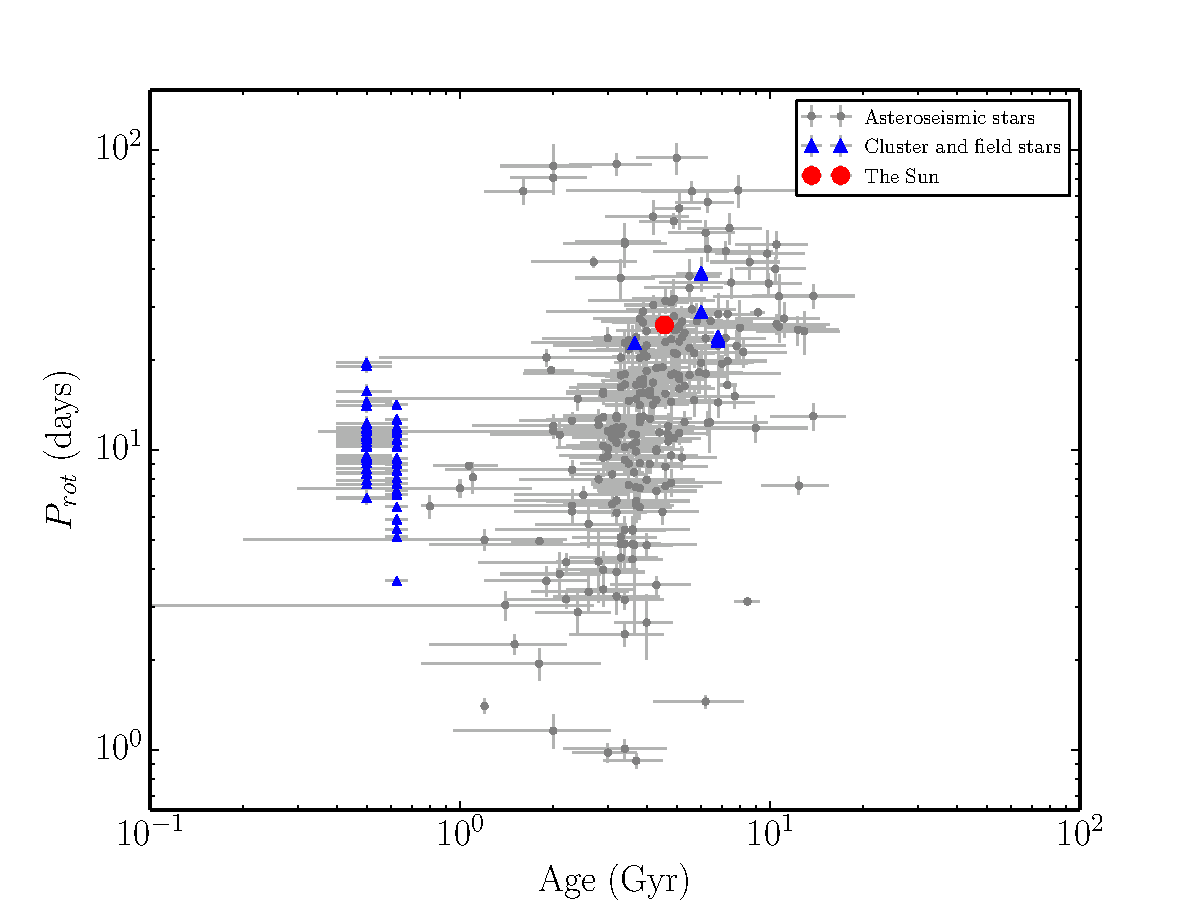
\includegraphics[width=6in, clip=true]{figures/p_vs_a_paper2.pdf}
\caption[Period vs age for \kepler\ stars]{Photometric rotation period vs age
for \nastero$~$ {\it Kepler} targets (grey circles) plus cluster and field
stars (blue triangles). The Sun is shown as a red circle.
\label{fig:p_vs_a}}
\end{center}
\end{figure*}

\begin{figure*}
\begin{center}
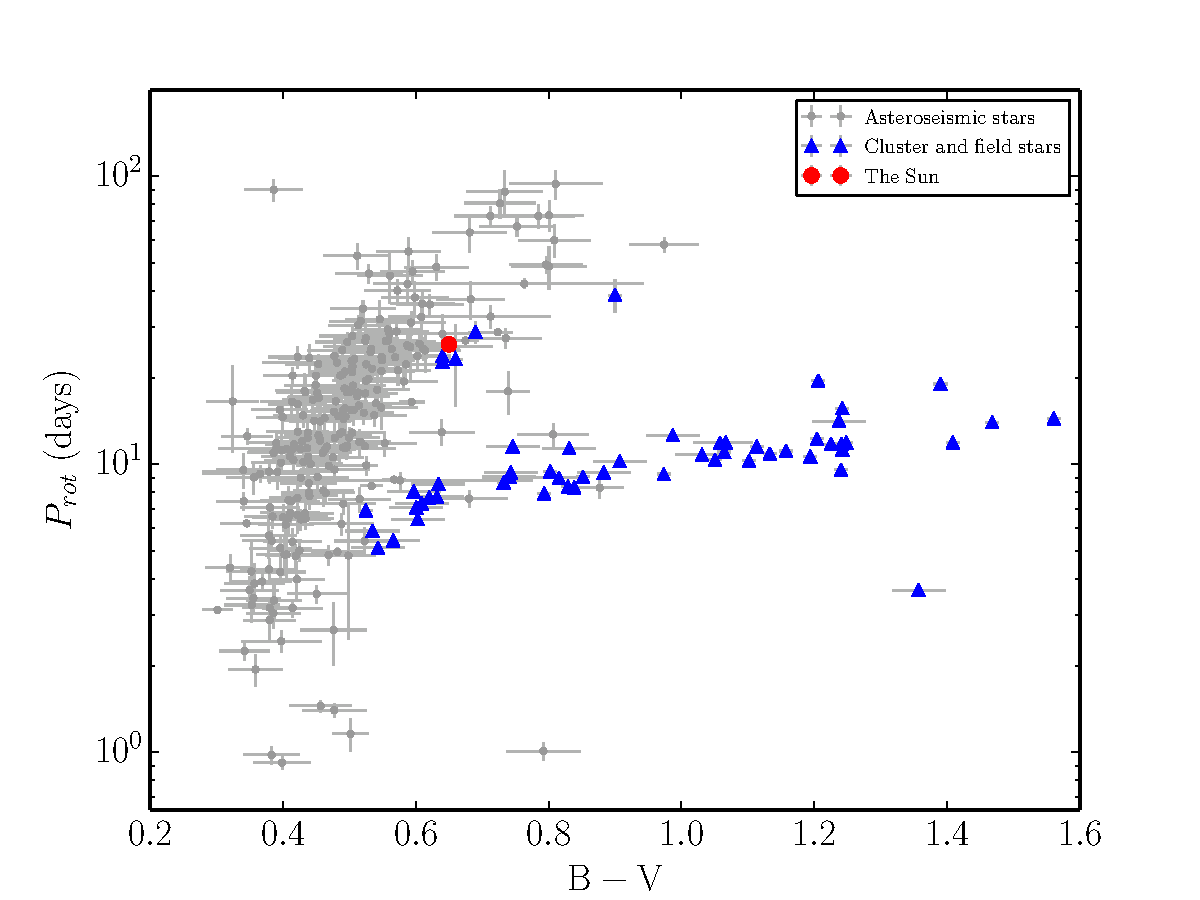
\includegraphics[width=6in, clip=true, trim=0 0 0.5in 0]{figures/p_vs_bv_paper2.pdf}
\caption[Period vs colour for \kepler\ stars]
{Photometric rotation period vs $B-V$ colour for the data described in figure
\ref{fig:p_vs_a}.
\label{fig:3d}}
\end{center}
\end{figure*}


\begin{table*}
\caption[Cluster data and references.]
{Clusters and References: (1) \citet{Dobbie2009},
	(2) \citet{CollierCameron2009}, (3) \citet{Perryman1998},
	(4) \citet{Radick1987}. \label{tab:clust}}
\begin{tabular}{lcccc}
\hline\hline
Cluster & Age (Gyr) & Number of stars & Age ref & Rotation period ref \\
\hline
Coma Ber & 0.5 $\pm$ 0.1 & 28 & 1 & 2 \\
Hyades & 0.625 $\pm$ 0.05 & 22 & 3 & 4 \\
\hline
\end{tabular}
\end{table*}

\begin{table*}
\caption[Field star data.]
{Rotation periods and $B-V$ colours for field stars with precise
	ages.
Notes: \citet{Davies2014} measured internal rotation periods for 16 Cyg A and B
using asteroseismology.
However, this is likely to be close to the surface rotation value.
Rotation periods for and $\alpha$ Cen A and B were measured
from variation in chromospheric emission lines.
High-resolution spectropolarimetric observations were used to measure
a rotation period for 18 Sco.
The age of 16 Cyg AB was measured with asteroseismology.
18 Sco's age measurement was based chiefly on an asteroseismic analysis,
however its rotation period was used as an additional constraint, so the age
estimate is not entirely independent of rotation period for this star.
An age for the $\alpha$ Cen system was estimated from spectroscopic
observations with additional seismic constraints.
References: a = \citet{Metcalfe2012}, b = \citet{Davies2014}, c =
\citet{Moffett1979}, d = \citet{Li2012}, e = \citet{Petit2008}, f =
\citet{Mermilliod1986}, g = \citet{Bouvier2010}, h = \citet{Donahue1996}, i =
\citet{Cox2000}, j = \citet{Bazot2012}, k = \citet{Yildiz2007}, l =
\citet{Hallam1991}, m = \citet{Dumusque2012}..
\label{tab:field}}

\begin{tabular}{lcccc}
\hline\hline
{ID} & {age} & {\prot} & {$B-V$} & References\\
\hline
16 Cyg A & 6.8 $\pm$ 0.4 & 23.8 $^{+1.5}_{-1.8}$ & 0.66 $\pm$ 0.01 &
a, b, c \\
16 Cyg B & 6.8 $\pm$ 0.4 & 23.2 $^{+11.5}_{-3.2}$ & 0.66 $\pm$ 0.01 &
a, b, c \\
18 Sco & 3.7 $\pm$ 0.2 & 22.7 $\pm$ 0.5 & 0.64 $\pm$ 0.01 &
d, e, f \\
The Sun & 4.568 $\pm$ 0.001 & 26.09 $\pm$ 0.1 & 0.65 $\pm$ 0.001 &
g, h, i \\
$\alpha$ Cen A & 6 $\pm$ 1 & 28.8 $\pm$ 2.5 &
0.69 $\pm$ 0.01 &
j, k, l, f \\
$\alpha$ Cen B & 6 $\pm$ 1 & 38.7 $\pm$ 5.0 &
0.90 $\pm$ 0.01 &
j, k, m, f \\
\hline
\end{tabular}
\end{table*}

\section{Calibrating the Gyrochronology relation}
\label{sec:gyro_cal}

\subsection{The model}

The \nastero$~$asteroseismic stars in our sample have $B-V$ colours converted
from effective temperatures, photometric rotation periods,
asteroseismic ages, and asteroseismic surface gravities.
Each measurement of these properties is assumed to be independent with an
associated Gaussian uncertainty.
Not all of the cluster stars added to our sample have \logg$~$values; however,
since we only use \logg$~$to separate the populations of subgiants and dwarfs
(and we assume that the cluster stars are dwarfs) this should not affect our
results.
Following the treatment of \citet{Barnes2007} and \citet{Mamajek2008},
rotation period was treated as the independent variable throughout the
modelling process.

Hot stars and subgiants follow a different gyrochronology relation to MS
dwarfs.
Stars with effective temperatures above the Kraft-break, $T_{\rm{eff}}
\sim$ 6250 K, \citep{Kraft1967} do not have a thick convective envelope and
cannot support a strong magnetic dynamo, so do not spin down appreciably
during their MS lifetimes.
Subgiants spin down rapidly as they expand due to angular momentum
conservation and thus diverge from the gyrochronological mass-period-age
plane.
The point in their evolution at which they depart, the `gyrochronological MS
turn off', is difficult to define.
Classically, MS turnoff is defined as the hottest point on a star's path on
the HR diagram (before it ascends the giant branch) but theory predicts that
evolving stars begin the process of spinning down relatively slowly after
leaving the classically defined MS \citep{Vansaders2013}.
For this reason we chose a very simple definition of MS turnoff: we defined
a \logg$~$boundary of \subcut to mark the transition between dwarfs and
giants.
We tried a range of boundary values and found that \subcut minimised subgiant
contamination whilst maximising the cool dwarf sample.  % referee
It was also necessary to use a mixture model to account for misclassified
subgiants---without it, subgiant contamination significantly biased the
resulting fit.
We did not exclude hot stars and subgiants from our sample during the
modelling process, we modelled all three populations simultaneously.
This allowed for the fact that stars have some probability mass lying in all
three regimes due to their large observational uncertainties.

Hot MS stars were defined as those with $B-V$ $<$ 0.45, corresponding to
\teff$~\approx$ 6250 K for solar metallicity and \logg.
Since there is no dependence of rotation period on age for massive MS stars,
their rotation periods were modelled as a normal distribution with mean and
standard deviation, $Y$ and $V$, as free parameters.
Subgiant rotation periods \emph{do} depend on age and $T_{\rm{eff}}$.
However, since the rotational properties of these stars are not interesting for
the purposes of gyrochronology calibration, we also modelled them with
a normal distribution with mean and standard deviation, $Z$ and $U$, as free
parameters.
We used a mixture model for the remaining population of stars, consisting of
cool dwarfs and misclassified, contaminating subgiants.
The subgiants were treated as if their rotation periods had been drawn from
a background normal distribution with mean and standard deviation, $X$ and
$U$, again inferred from the data and another parameter, $Q$, the
probability of each star belonging to that background population.
The results of this analysis were not particularly sensitive to the choice of
distribution for the hot stars and subgiants.
These models were put in place so that we did not have to throw any data
away and we could model everything at once.
This was important because stars were classified according to their observed
temperatures and \logg s, which are noisy.
Due to the large uncertainties on \teff$~$and \logg, each star therefore has some
probability of being a subgiant, some of being a cool dwarf and some of
being a hot star.
By throwing away data, one could accidentally throw away a misclassified star.
We avoid this problem by modelling all stars simultaneously and taking a
probabilistic approach to classification.
Inferences made about the parameters of the normal distributions used to model
subgiants and hot stars were not of particular interest for the purposes of
gyrochronology calibration.
We decided to use simple normal distributions rather than more physically
motivated models in order to remain as model--independent as
possible.
Figure \ref{fig:logg_vs_t} shows \logg$~$vs \teff$~$for the asteroseismic stars.
Stars classified as cool dwarfs are shown in black, hot dwarfs in red and
subgiants in blue.

\begin{figure*}
\begin{center}
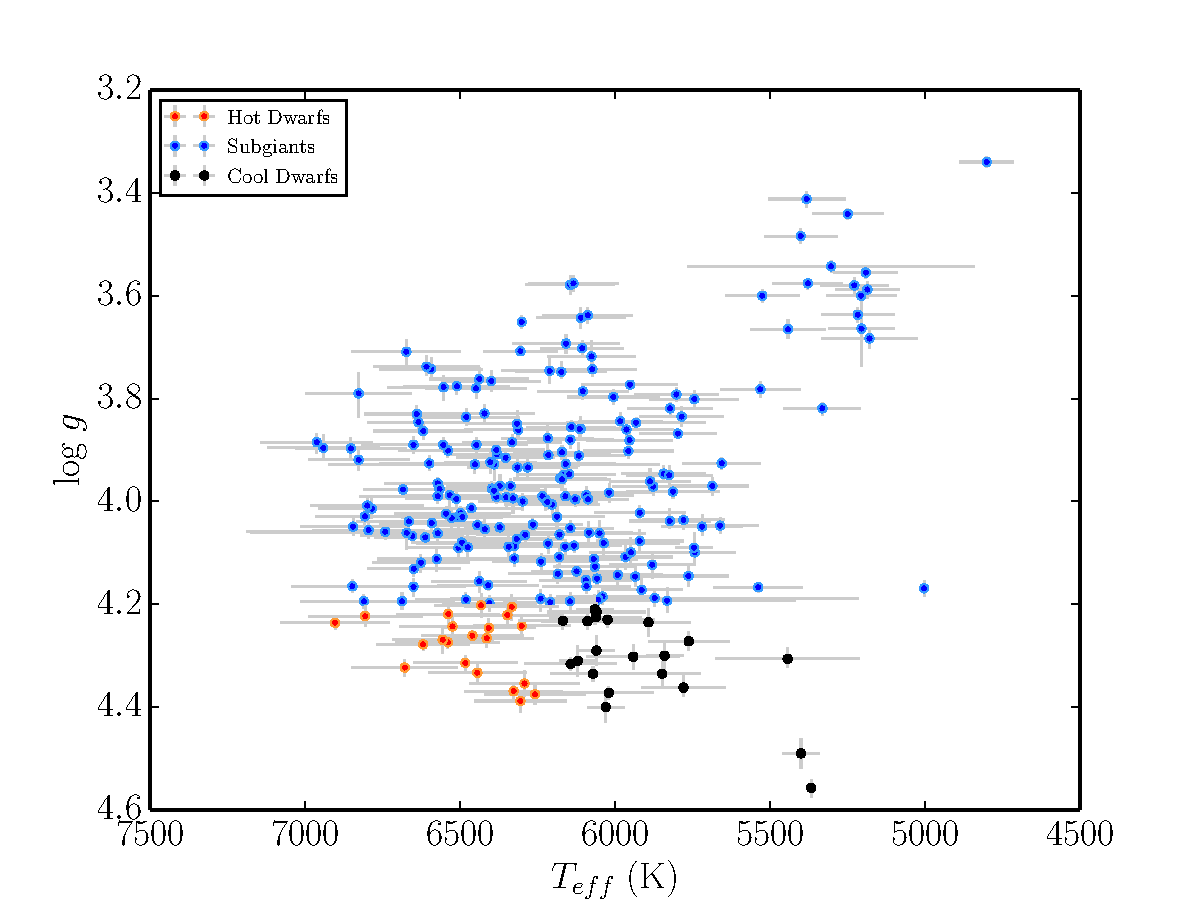
\includegraphics[width=6in, clip=true, trim=0 0 0.5in 0]{figures/logg_vs_t_paper.pdf}
\caption[\logg vs T$_{\mathrm{eff}}$ for \kepler\ stars]
{\logg$~$vs \teff$~$for the \nastero$~$asteroseismic stars. Hot dwarfs
with \teff$~>$ 6250 K and \logg$~>$ \subcut are red, subgiants with \logg$~<$
\subcut are blue. Only the black cool dwarfs with \teff$~<$ 6250 K and
\logg$~<$ \subcut are expected to follow the gyrochronology relation in
equation \ref{eq:Barnes2007_2}.
\label{fig:logg_vs_t}}
\end{center}
\end{figure*}

Ideally both the hot star ($B-V$ $<$ 0.45) and subgiant (\logg $<$ \subcut)
boundaries would be free parameters in our model.
However, since these two populations were modelled with a relatively
unconstraining normal distributions, these boundary parameters would not be
well behaved.
Both would be pushed to higher and higher values until all stars were modelled
with a normal distribution.
In order to avoid this problem, we fixed these two boundaries.
A future analysis could avoid the assumption that the gyrochronology relation
is infinitely narrow and assign it some intrinsic width, which would also be
a free parameter.

We postulate that there is a deterministic relationship between the `true'
rotation period of a cool MS star and its `true' age and colour, described by
equation \ref{eq:Barnes2007_2} (by `true' we mean the value an observable
property would take, given extremely high signal-to-noise measurements).
Rotation period also depends on \logg$~$since this property determines whether
a star falls in the dwarf or subgiant regime.

In what follows we use $P$ to denote rotation period and define
$\mathbf{w} = (age, B-V,~\log~g)$ as the vector of additional observational
properties.
Observations are denoted as \ph$~$and $\hat{\mathbf{w}}_n$ and the unobserved
(latent), `true' parameters as $P_n$ and $\mathbf{w}_n$ for stars $1,...,N$.

In order to explore the posterior Probability Density Functions (PDFs) of
the model parameters, $\theta$, conditioned on a set of noisy observations,
$\{\hat{P}_n, \hat{\mathbf{w}}_n\}$, it was necessary to marginalise over the
latent parameters, $\{P_n, \mathbf{w}_n\}$.
This is because the model parameters, $\theta$ are conditionally dependent on
the `true' values of rotation period and colour, \emph{not} the observed
values themselves.
The observed values are only conditionally dependent on the `true' values.
In order therefore to infer the values of the model parameters using the
observed values of rotation period and colour, it was necessary to marginalise
over the latent parameters.  % referee
This is another example of hierarchical inference.
Assuming all measurements are independent, the marginalised likelihood can be
written
\begin{equation}
	p(\{\hat{P}_n,\hat{\w}_n\}|\theta) =
	\prod_{n=1}^{N} \int p(\hat{P}_n,\hat{\w}_n,P_n,\w_n|\theta)
	{\rm d}P_n {\rm d}\w_n.
\label{eq:fulll}
\end{equation}
The joint probability, on the right hand side of this equation, can be
factorised as
\begin{align}
	p(\hat{P}_n,\hat{\w}_n,P_n,\w_n|\theta) = & \\
	p(P_n\,| & \,\w_n,\theta)
	p(\hat{P}_n\,|\,P_n)\,p(\hat{\w}_n\,|\,\w_n)p(\w_n),
\nonumber
\end{align}
where we have utilised the fact that the observations, \ph$~$and \wh$~$are
{\it conditionally independent} of the model parameters, $\theta$: they only
depend on $\theta$ through the latent parameters, $P_n$ and $\w_n$.
The above integral can  be written
\begin{eqnarray} \label{eq:lhf_gyro}
	p(\{\hat{P}_n,\hat{\w}_n\}|\theta) \propto &
	\prod_{n=1}^{N} \int p(\w_n|\hat{\w}_n) {\rm d}\w_n \\ \nonumber
	& \int p(P_n|\w_n,\theta) p(\hat{P}_n\,|\,P_n) {\rm d}P_n,
\end{eqnarray}
where we have used Bayes' theorem:
$p(\w_n|\hat{\w}_n) \propto p(\hat{\w}_n|\w_n)p(\w_n)$.
The outer integral is the same for hot dwarfs, cool dwarfs and subgiants
alike.
In our model, the likelihood function---the probability of the `true' rotation
period given the `true' observed parameters and the model parameters,
$p(P_n|\w_n, \theta)$, is different in each regime because a different
generative process is responsible for producing rotation periods.
For cool dwarfs ($B-V$ $>$ 0.45 and \logg$~>$ \subcut) the likelihood function
can be written
\begin{eqnarray} \label{eq:codw}
p(P_n|\w_n,\theta) &=&
    (1-Q)~\delta \left (P_n - f_\theta(\w_n)\right) \\ \nonumber
    && +\quad Q\,\left(\sqrt{2\pi U^2}\right)^{-1/2} \\ \nonumber
    &&	~\exp\left({-\frac{(P_n-X)^2}{2U^2}}\right),
\end{eqnarray}
where $Q$ is the probability that a star is drawn from the population of
misclassified subgiants and
\begin{eqnarray}
f_\theta(\w_n) = A^n \times a(B-V - c)^b
\label{eq:blank}
\end{eqnarray}
is the gyrochronology relation.
For hot dwarfs ($B-V$ $<$ 0.45 and \logg$~>$ \subcut) the likelihood function
is:
\begin{eqnarray}
p(P_n\,|\,\w_n,\theta) = \left(\sqrt{2\pi V^2}\right)^{-1/2}~
\exp\left({-\frac{(P_n-Y)^2}{2V^2}}\right),
\label{eq:hot_dwarfs}
\end{eqnarray}
and for subgiants,
\begin{eqnarray}
p(P_n\,|\,\w_n,\theta) = \left(\sqrt{2\pi W^2}\right)^{-1/2}~
\exp\left({-\frac{(P_n-Z)^2}{2W^2}}\right).
\label{eq:subgiants}
\end{eqnarray}

We used hierarchical inference to account for observational uncertainties,
following the method of \citet{Hogg2010}, also used by
\citet{Foreman-Mackey2014}, \citet{Rogers2014}, \citet{Morton2014} and
\citet{Demory2014}.
We computed the likelihood for each star (equation \ref{eq:lhf_gyro}), up to
an unimportant constant using a sampling approximation.
The values of \ph$~$and \wh$~$with uncertainties, $\sigma_P$ and
$\sigma_{\mathbf{w}}$, reported in catalogues provide constraints on the
posterior probability of those variables, under a choice of prior PDF,
$p_0(\hat{\mathbf{w}}_n)$.
Ideally, these catalogues would provide posterior PDF samples, not just point
estimates, which we could use directly.
i.e. samples from
\begin{equation}
	p(\mathbf{w}_n|\hat{\mathbf{D}}_n) =
	\frac{p(\hat{\mathbf{D}}_n|\mathbf{w}_n)p_0(\mathbf{w}_n)}
	{p_0(\hat{\mathbf{D}}_n)},
\end{equation}
where $p(\hat{\mathbf{D}}_n|\w_n)$ is the likelihood of the data,
$\hat{\mathbf{D}}_n$ (in this case,
the set of {\it Kepler} lightcurves plus spectroscopic \teff$~$and
\feh$~$measurements), given the model parameters, $\mathbf{w}_n$.
$p_0(\mathbf{w}_n)$ is an uninformative prior PDF, chosen by the
fitter \citep[][used a flat prior PDF in age and \logg]{Chaplin2014}.
In the absence of posterior PDF samples\footnote{Posterior PDF samples
for asteroseismic parameters are now beginning to be published and will be made
available in future publications.} we generated our own from Gaussian
distributions with means, \wh$~$and standard deviations, $\sigma_{\mathbf{w}}$.
$J$ posterior samples were generated for each star (we used $J$ = 500):
% non referee
% \begin{eqnarray}
% \w_n^{(j)} &\sim& p(\w_n\,|\,\hat{\w}_n),
% \end{eqnarray}
\begin{equation}
\w_n^{(j)} \sim p(\w_n\,|\,\hat{\w}_n),
\end{equation}
and were used to evaluate $p(\mathbf{w}_n|\hat{\mathbf{w}}_n)$ up to a
normalisation constant.
% We then evaluated the marginalized likelihood for a single star as follows
Using these samples we computed the marginalised likelihood for a single
star as follows,
\begin{align}
% 	p(\hat{P}_n,\hat{\w_n}\,|\,\theta) \approx \frac{1}{J_n}
% 	\sum_{j=1}^{J_n}p(\hat{P}_n\,|\,\mathbf{w}_n^{(j)},\theta).
	% p(\hat{P}_n,\hat{\w_n}\,|\,\theta) \approx \frac{1}{J_n}
	% \sum_{j=1}^{J_n}p(P_n\,|\,\mathbf{w}_n^{(j)},\theta)p(\hat{P}_n|P_n).
	p(\hat{P}_n,\hat{\w_n}\,|\,\theta) \approx \frac{1}{J_n}
	\sum_{j=1}^{J_n}p(\hat{P}_n\,|\,\mathbf{w}_n^{(j)},\theta) \quad.
\end{align}
The argument inside this sum is given by the integral
% \begin{eqnarray}
% p(\hat{P}_n\,|\,\mathbf{w}_n^{(j)},\theta) =
%     \int p(P_n|\w_n,\theta) p(\hat{P}_n\,|\,P_n) {\rm d}P_n \quad.
% \end{eqnarray}
\begin{equation}
p(\hat{P}_n\,|\,\mathbf{w}_n^{(j)},\theta) =
    \int p(P_n|\w_n,\theta) p(\hat{P}_n\,|\,P_n) {\rm d}P_n \quad.
\end{equation}
Assuming that the period uncertainties are Gaussian with mean $\hat{P}_n$
and variance ${\sigma_n}^2$, this integral can be evaluated analytically for
each population.
For example, starting from equation~\ref{eq:codw} the result for the cool
dwarfs is
\begin{eqnarray} \label{eq:cool_dwarfs}
p(\hat{P}_n\,|\,\mathbf{w}_n^{(j)},\theta) &=&
    \frac{1-Q}{\sqrt{2\,\pi\,{\sigma_n}^2}} \exp\left( -
        \frac{\left[\hat{P_n} - f_\theta (\w_n^{(j)}) \right] ^2}
             {2\,{\sigma_n}^2}\right) \nonumber\\
    && +
    \frac{Q}{\sqrt{2\,\pi\,(U^2 + {\sigma_n}^2)}} \exp\left( -
        \frac{[\hat{P_n} - X] ^2}{2\,[U^2 + {\sigma_n}^2]}\right) \quad.
\end{eqnarray}
A similar result can be derived for the other populations.

Finally, using these analytic results for the inner integral, the
marginalised log-likelihood from equation \ref{eq:lhf_gyro} becomes
\begin{eqnarray}
	\log p(\{\hat{P}_n,\hat{\w}_n\}\,|\,\theta) \approx & \\ \nonumber
    & \log \mathcal{Z} + \sum_{n=1}^N
	\log \left[ \sum_{j=1}^{J_n}p(\hat{P}_n\,|\,\mathbf{w}_n^{(j)},
\theta) \right ]
\end{eqnarray}
where $\mathcal{Z}$ is an irrelevant normalisation constant.
We used {\tt emcee} \citep{Foreman-Mackey2013}, an affine invariant, ensemble
sampler Markov Chain Monte Carlo (MCMC) algorithm, to explore the posterior
PDFs of the model parameters, $\theta$.
Flat prior PDFs were used for each parameter.
Following the above method, a likelihood was computed as follows:
\begin{itemize}
	\item For each star, $J$ samples were drawn from three normal
		distributions: one in colour, one in age and one in \logg,
		where the means and standard deviations of those distributions
		were the observed values and uncertainties.
		This step was performed just once and the
		following steps were performed for each likelihood evaluation.
	\item For those samples that fell in the cool dwarf regime
		($B-V$ $>$ 0.45 and \logg$~>$ \subcut), model rotation
		periods were both calculated using equation
		\ref{eq:Barnes2007_2} and assigned the value of parameter $X$.
% 		In the case that the sample was better described by equation
% 		\ref{eq:Barnes2007_2} than by the normal distribution with mean
% 		and standard deviation $X$ and $U$, that sample
		Likelihoods for the two model rotation periods were then
		evaluated using a Gaussian mixture model
		likelihood function (equation \ref{eq:cool_dwarfs}).
	\item For the samples that fell in the hot dwarf ($B-V$ $<$ 0.45 and
		\logg$~>$ \subcut) and subgiant (\logg$~<$ \subcut) regimes,
		likelihoods were calculated by comparing observed rotation
		periods with the model rotation periods for the two
		populations: $Y$ and $Z$.
	\item The total log-likelihood for each star was calculated as the
		sum of the log-likelihoods of each of the $J$ samples.
	\item Finally, the sum of individual star log-likelihoods
		provided the total log-likelihood.
\end{itemize}

\section{Results and Discussion}
\label{sec:results}

\begin{table}
	\caption[Individual cluster results.]
{Median values of $a$, $b$ and $n$ for individual clusters
		(see equation \ref{eq:Barnes2007_2}).  % referee
\label{tab:cluster_results}}

\begin{center}
\begin{tabular}{lccc}
\hline\hline
{Parameter} & {Coma Berenices} & {Hyades} \\
\hline
a & $0.417^{+0.08}_{-0.07}$ & $0.312^{+0.04}_{-0.06}$ \\
b & $0.271^{+0.05}_{-0.06}$ & $0.410^{+0.05}_{-0.04}$ \\
n & $0.542 \pm 0.03$ & $0.599^{+0.03}_{-0.02}$ \\
\hline
\end{tabular}
\end{center}
\end{table}

A gyrochronology relation was initially fit to the asteroseismic stars, the
field stars and four clusters (Hyades, Coma Berenices, Praesepe and NGC 6811)
all together.
However, this resulted in extremely multi-modal posteriors PDFs for
$a$, $b$ and $n$.
After fitting a separate relation to various subsets of the data, it became
evident that a lower value of $b$ was preferred by NGC 6811,
i.e. the slope of the $\log(\mathrm{period})-\log(B-V-c)$ relation was
shallower for NGC 6811 than for the Hyades, Coma Berenices and Praesepe.
% referee
The reason for NGC 6811's shallower slope is currently unknown, however the
slope increased slightly after more quarters of \kepler\ data were included
in the rotation period measurement process (Meibom, private communication), so
this may be due to systematic uncertainties on the rotation periods.
We therefore exluded NGC 6811 from our sample and attempted to fit
a relation to the remaining data.
Multi-modal posterior PDFs were still produced however, until Praesepe was
also removed from the sample.
The reason for this multi-modality is unclear, but we tentatively attribute
it to Praesepe preferring a different value for the colour discontinuity, $c$,
to the Hyades and Coma Berenices.  % referee
We calculated the likelihood for Praesepe, plus the field stars (to provide
the age dependence) with two different values of $c$: $0.45$ and $0.5$,
finding a higher likelihood for $c=0.5$.
Since we do not fully understand the cause of this variation in $c$, and in
order to keep our model simple, we chose to also exclude Praesepe from
our final data set and fit a gyrochronology relation with $c=0.45$ to the
remaining data (asteroseismic stars, field stars, Hyades and Coma Berenices).
We also fitted relations with $c$ values ranging from 0.4 to 0.55 to this final
data set, finding that the results were relatively insensitive to variations
in this parameter (solar ages predicted from each best-fitting model were
consistent within uncertainties).
Individual fits to Hyades and Coma Berenices, plus the field stars are shown
in figures \ref{fig:CF45} and \ref{fig:HF45}.
Median values of $a$, $b$ and $n$ for the two clusters with their 16th and 84th
percentile uncertainties are provided in table
\ref{tab:cluster_results}.
Note that none of these parameters are fully consistent between the two
clusters.
% there seems to be some intrinsic scatter in the gyrochronology
% parameters.
The fact that each cluster seems to prefer a different value of $a$, $b$, $n$
and $c$ paints a concerning picture for this form of a gyrochronology relation
which assumes one set of parameters can be used to describe all stars.
It is likely that the inability of equation \ref{eq:Barnes2007_2} to fully
describe the observed properties of our sample of stars is due to the
simplifying assumptions that go into this relationship.
The fact that there is no dependence on metallicity, for example, may
contribute to the deficiencies of this model.
One might expect metallicity to have an effect on the rotational evolution of
a star since it impacts its internal structure.
We have not attempted to calibrate a metallicity-dependent gyrochronology
relation, because there are no precise metallicity measurements for the
majority of the {\it Kepler} stars, on which this study is chiefly based.
In addition, we anticipate that the majority of stars for which this new
gyrochronology relation will be most useful are {\it Kepler} stars, or stars
targeted by missions like {\it Kepler}, again, the majority of which are unlikely to
have precise metallicities.  % referee

\begin{figure}
\begin{center}
	\subfigure[Rotation period vs age and $B-V-c$ for the Hyades.]{
            \label{fig:CF45}
	    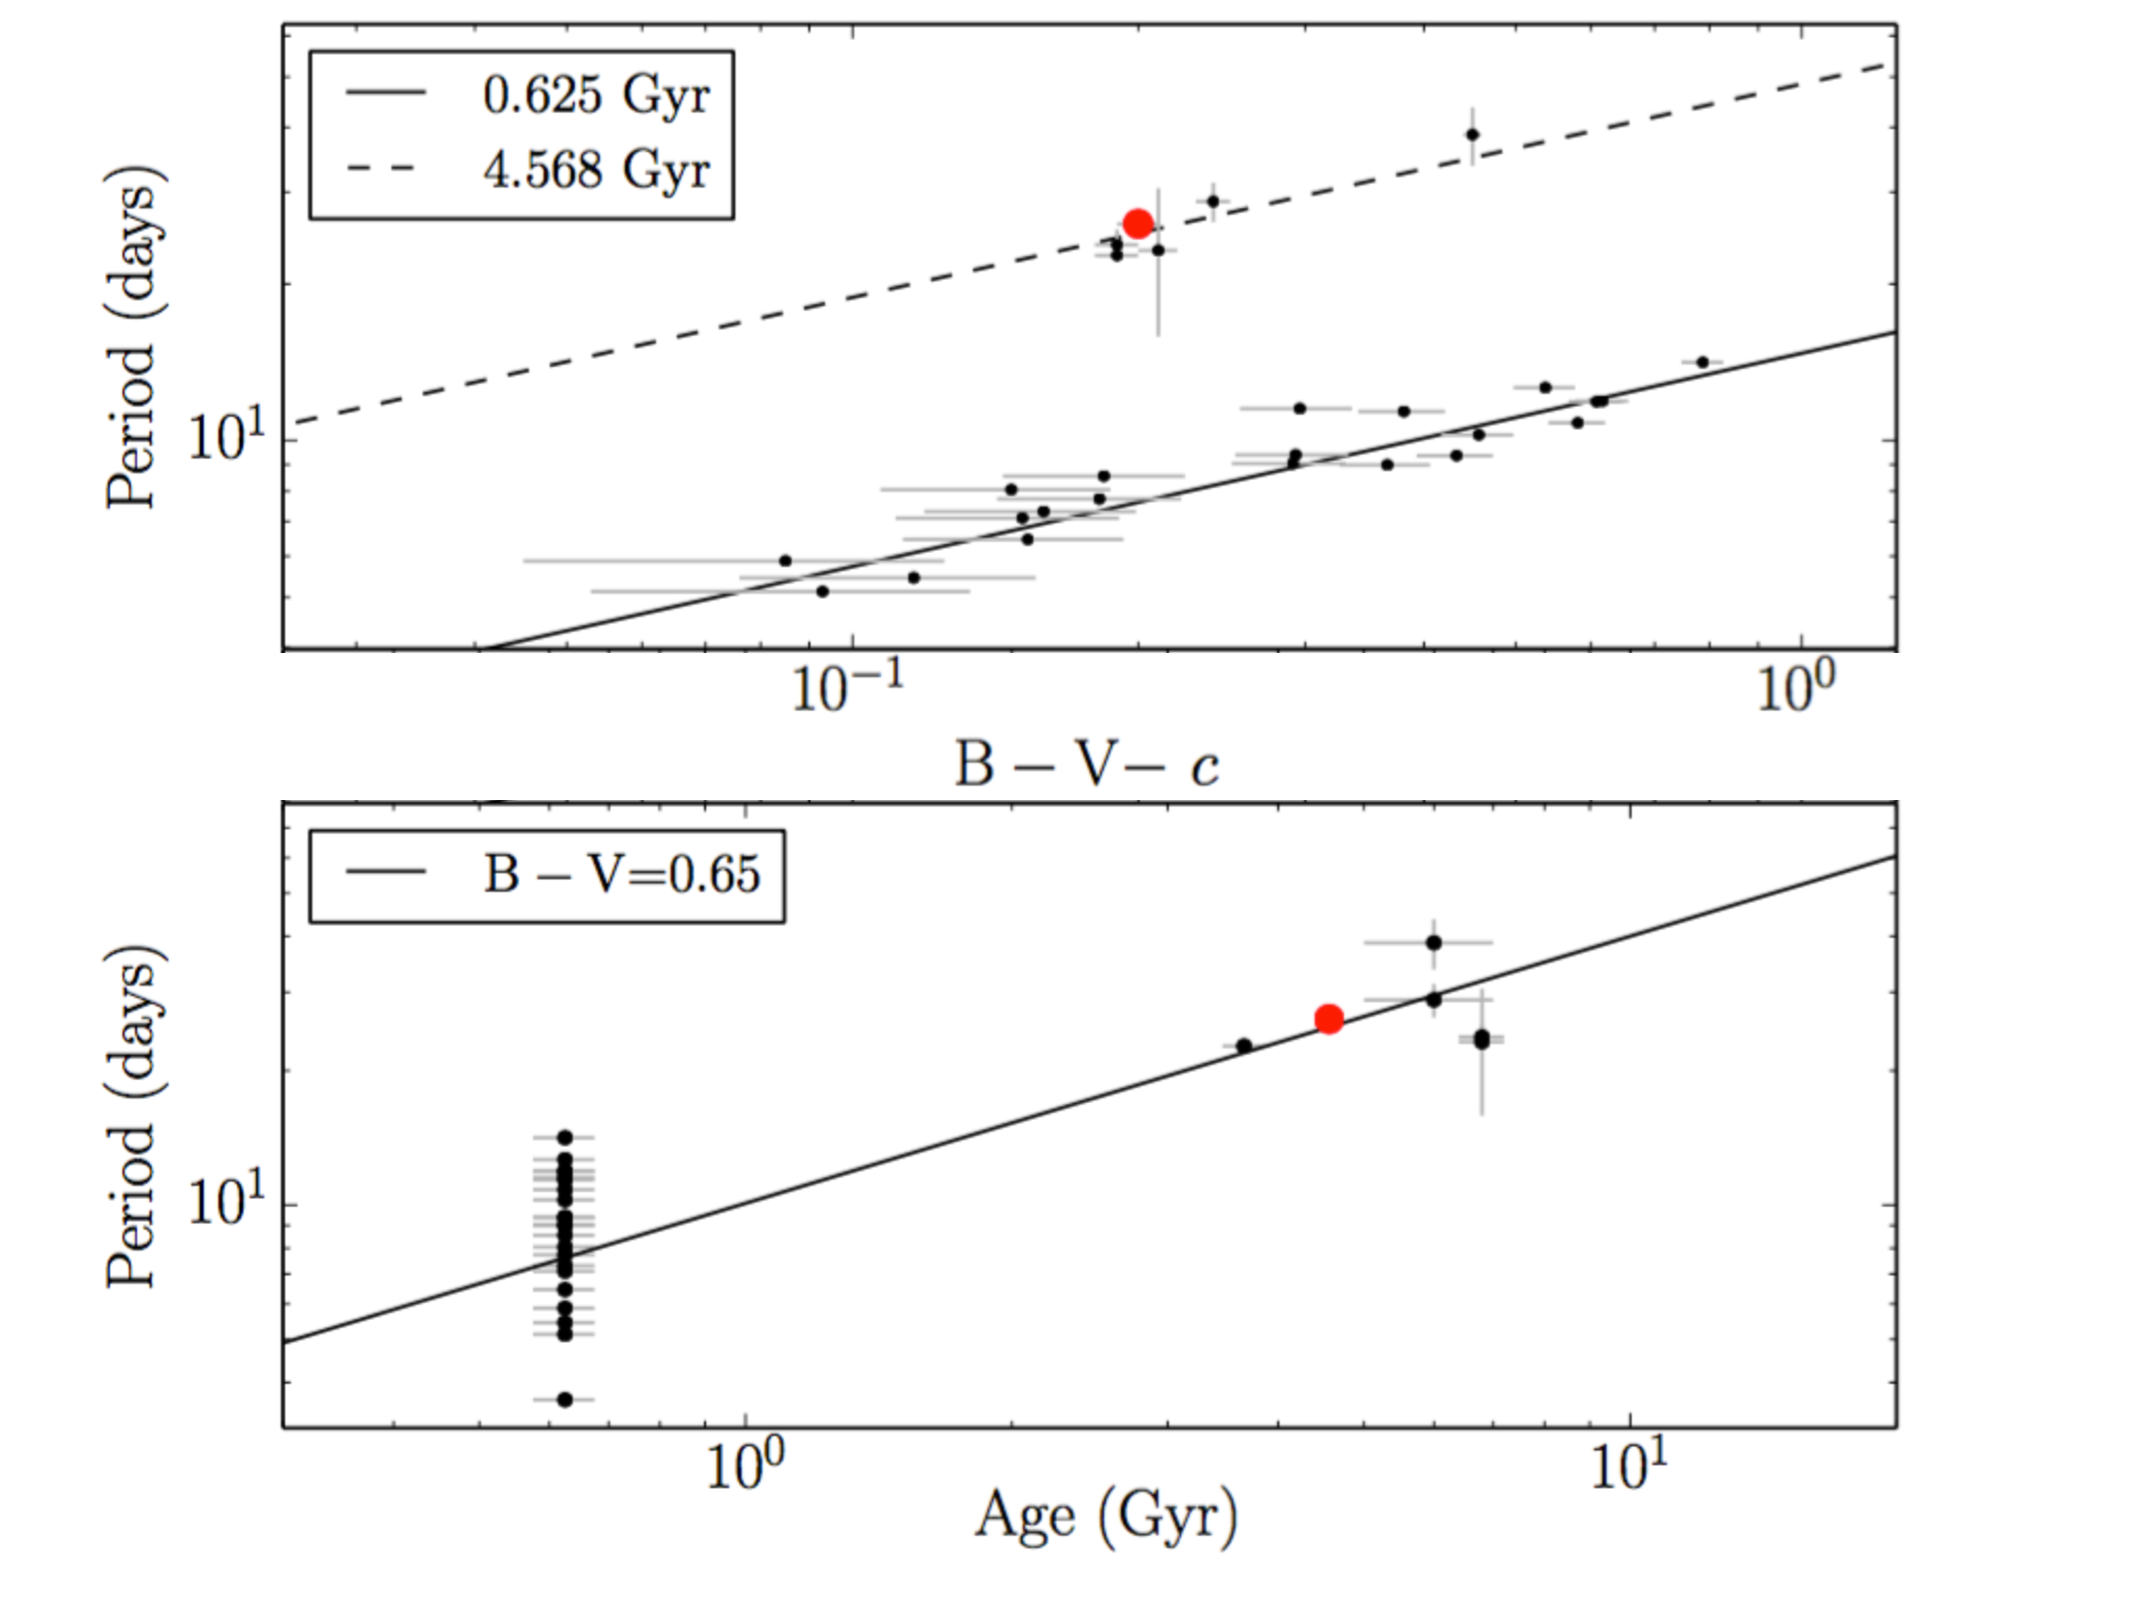
\includegraphics[width=4in]{figures/showHF45.pdf}
        }
	\subfigure[Rotation period vs age and $B-V-c$ for Coma Berenices.]{
            \label{fig:HF45}
	    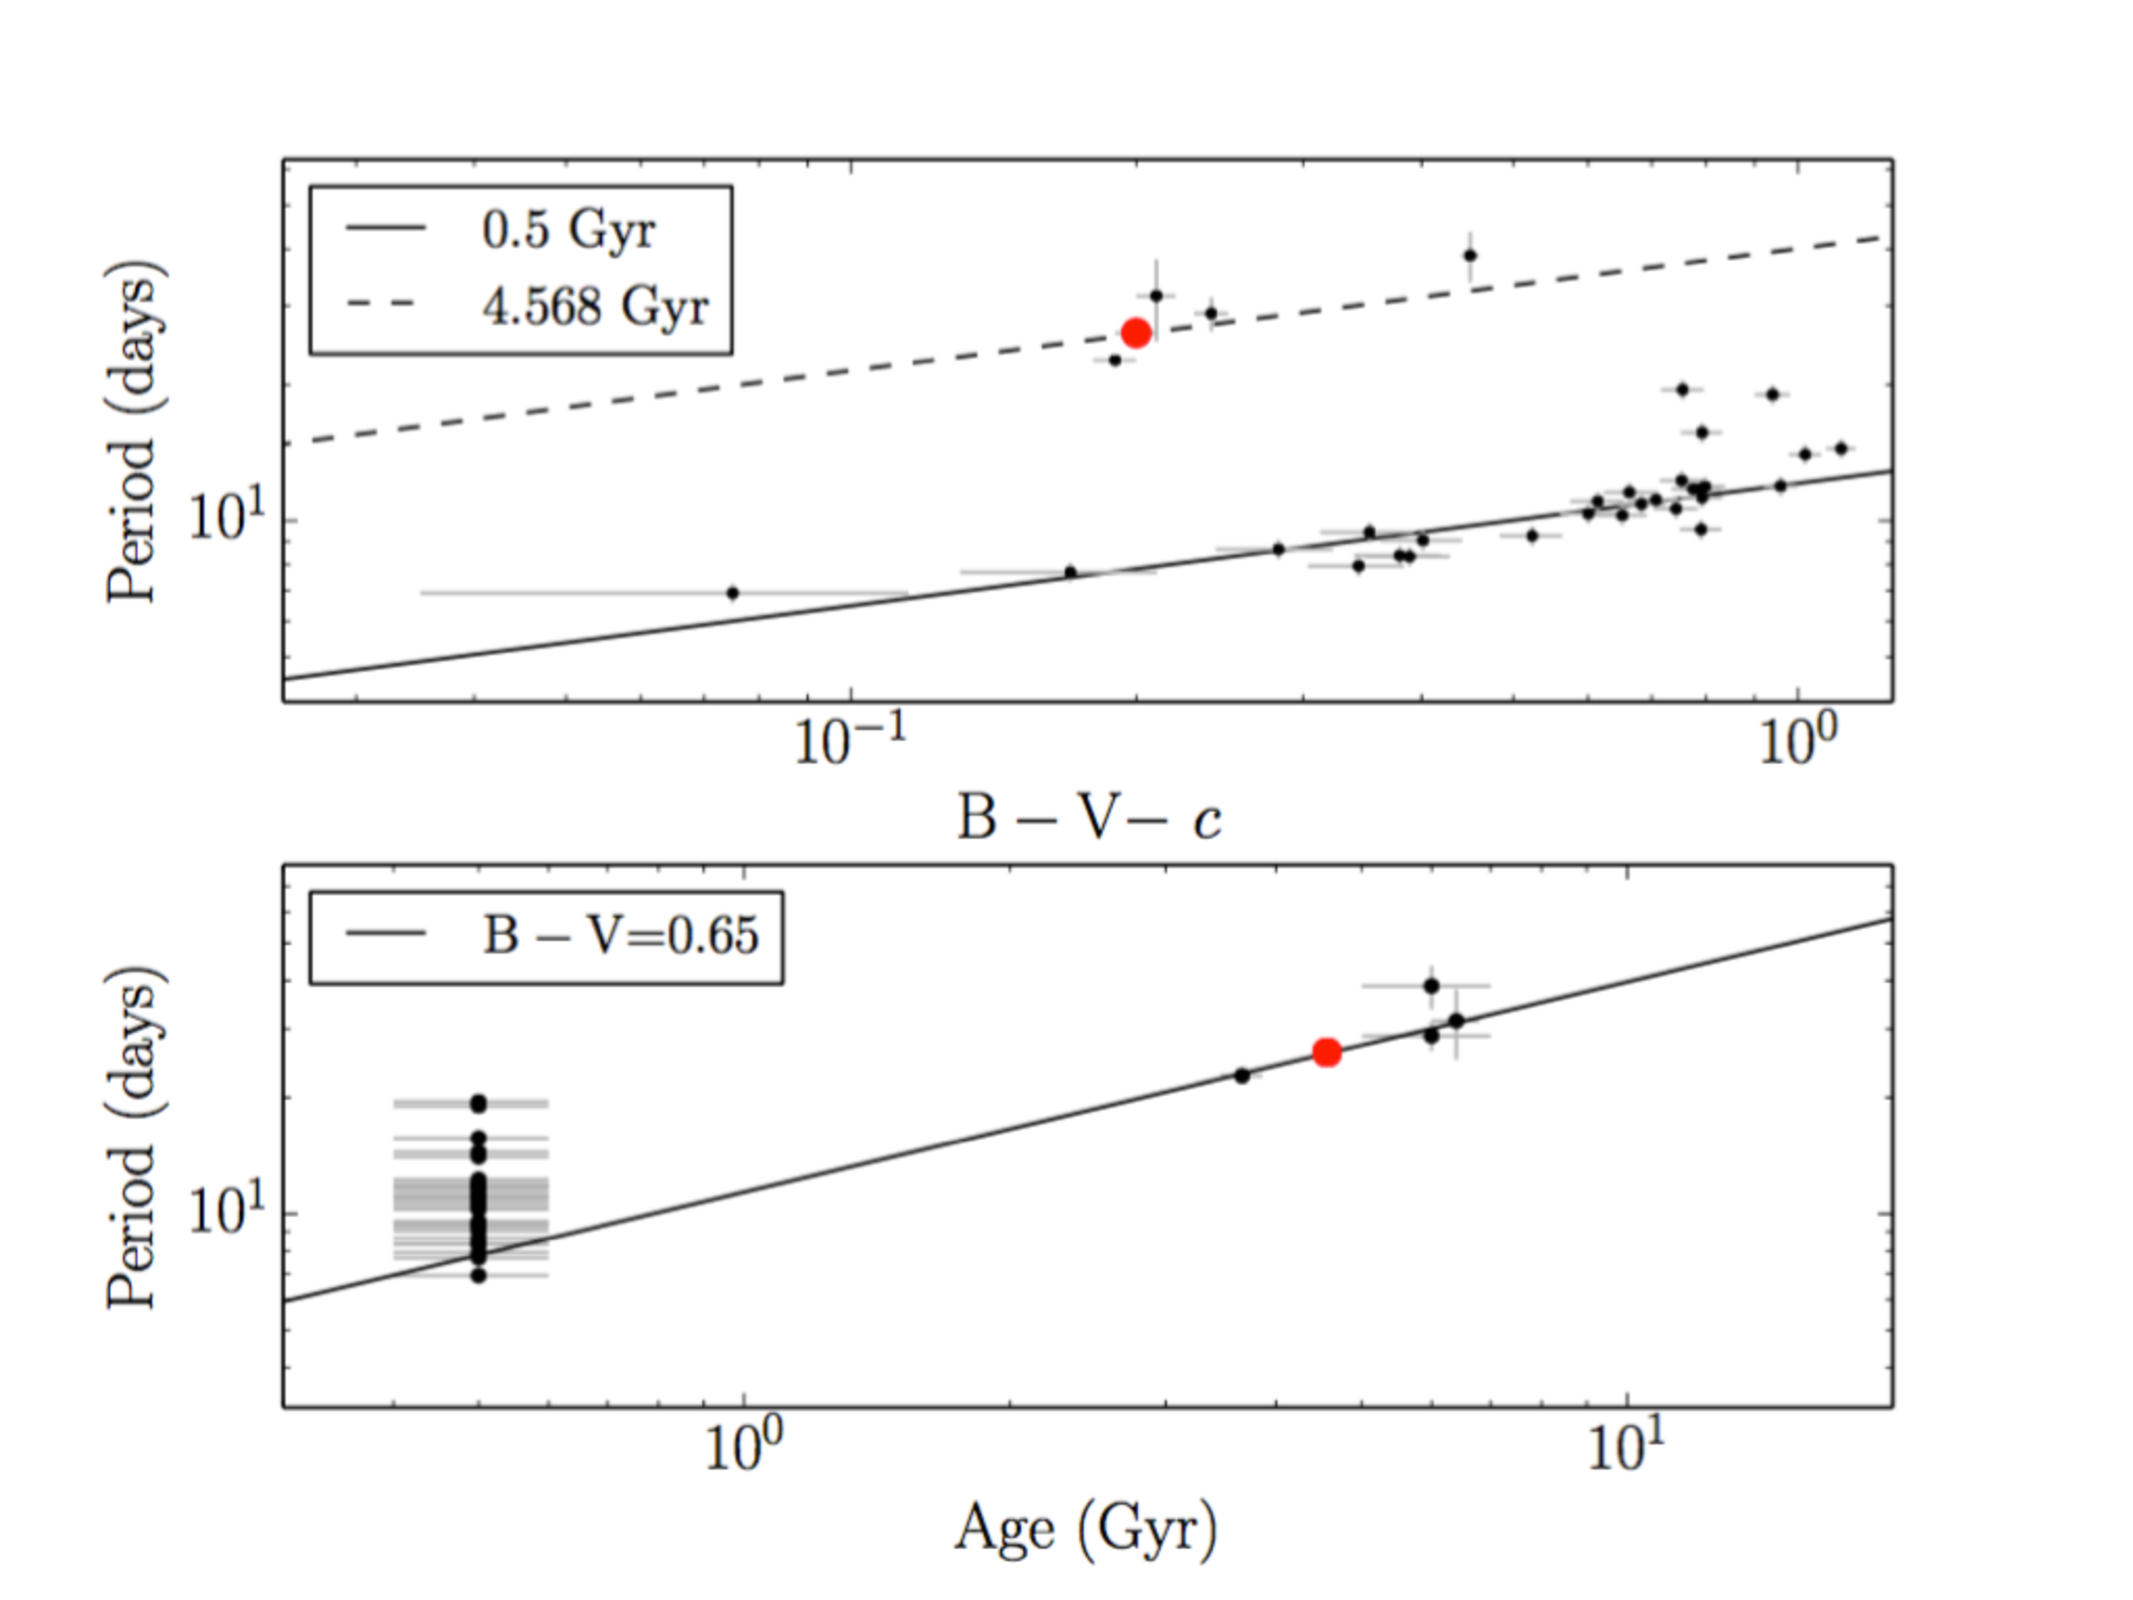
\includegraphics[width=4in]{figures/showCF45.pdf}
        }
    \end{center}
    \caption[Fits to age-rotation curves for individual clusters]
{ Individual fits to the clusters and field stars. The Sun is the
	    red point. The top figure shows rotation period vs `$B-V-c$' for
	    the Hyades (top) and Coma Berenices (bottom) with Solar and cluster
	    age isochrones. The bottom figure shows rotation period vs age
	    for the Hyades (top) and Coma Berenices (bottom) with the period-
	    age relation for a constant $B-V$ value of 0.65 (Solar $B-V$).
\label{fig:subfigures1}}
\end{figure}

\begin{table}
\caption[Nuisance parameter results]
{Median values of the parameters describing the populations of
	non-gyrochronological stars. \label{tab:nuisance}}

\begin{center}
\begin{tabular}{lccc}
\hline\hline
{Parameter} & {Symbol} & {Median value} \\
\hline
$\sigma_P (B-V > 0.45)$ & $U$ & \U$^{+\Uerrp}_{-\Uerrm}$ days \\
$\sigma_P (B-V < 0.45)$ & $V$ & \V$^{+\Verrp}_{-\Verrm}$ days \\
$\sigma_P (\log~g < 4.2)$ & $W$ & \W$^{+\Werrp}_{-\Werrm}$ days \\
% $X$ & \X$^{+\Xerrp}_{-\Xerrm}$ days \\
$\mu_P (B-V > 0.45)$  & $X$ & \X$\pm\Xerr$ days \\
$\mu_P (B-V < 0.45)$ & $Y$ & \Y$^{+\Yerrp}_{-\Yerrm}$ days \\
$\mu_P (\log~g < 4.2)$ & $Z$ & \Z$^{+\Zerrp}_{-\Zerrm}$ days \\
Giant fraction & $Q$ & \Q$^{+\Qerrp}_{-\Qerrm}$ \\
\hline
\end{tabular}
\end{center}
\end{table}

The resulting highest probability values of $a$, $b$ and $n$ from our fit to
the final data set, with 16th and 84th percentile uncertainties are
presented in table \ref{tab:constants}.
The additional parameters of our model, describing the distributions of hot
star and subgiant rotation periods, are presented in table \ref{tab:nuisance}.
The posterior PDFs of these parameters were all unimodal.
Note the value of $Q$, the parameter describing the fraction of misclassified
subgiants is $\Q^{+\Qerrp}_{-\Qerrm}$, i.e., based on our simple `\logg$=4.2$'
definition of MS turn-off, which left only 21 stars classified as cool dwarfs,
one or two of these are likely to be misclassified subgiants.
Marginalised posterior PDFs for the three gyrochronology parameters are shown
in figure \ref{fig:gyro_triangle} and the resulting relation between period and age
for stars of Solar-like colour is shown in figure \ref{fig:p_vs_a_solar}.
The relation between period and colour for Solar-age stars is shown in figure
\ref{fig:p_vs_bv_solar} and for a range of ages in figures
\ref{fig:gyro_5}-\ref{fig:8gyr}.
Note that we plot rotation period vs `$B-V-c$', producing a straight line, in
order to give a more intuitive understanding of the quality of the fit to the
data.
In figures \ref{fig:p_vs_a_solar} to \ref{fig:8gyr} we plotted 100 draws from
the posterior PDFs of the gyrochronology parameters as faint grey lines,
in order to demonstrate the widths and bimodal natures of these distributions.

\begin{figure*}
\begin{center}
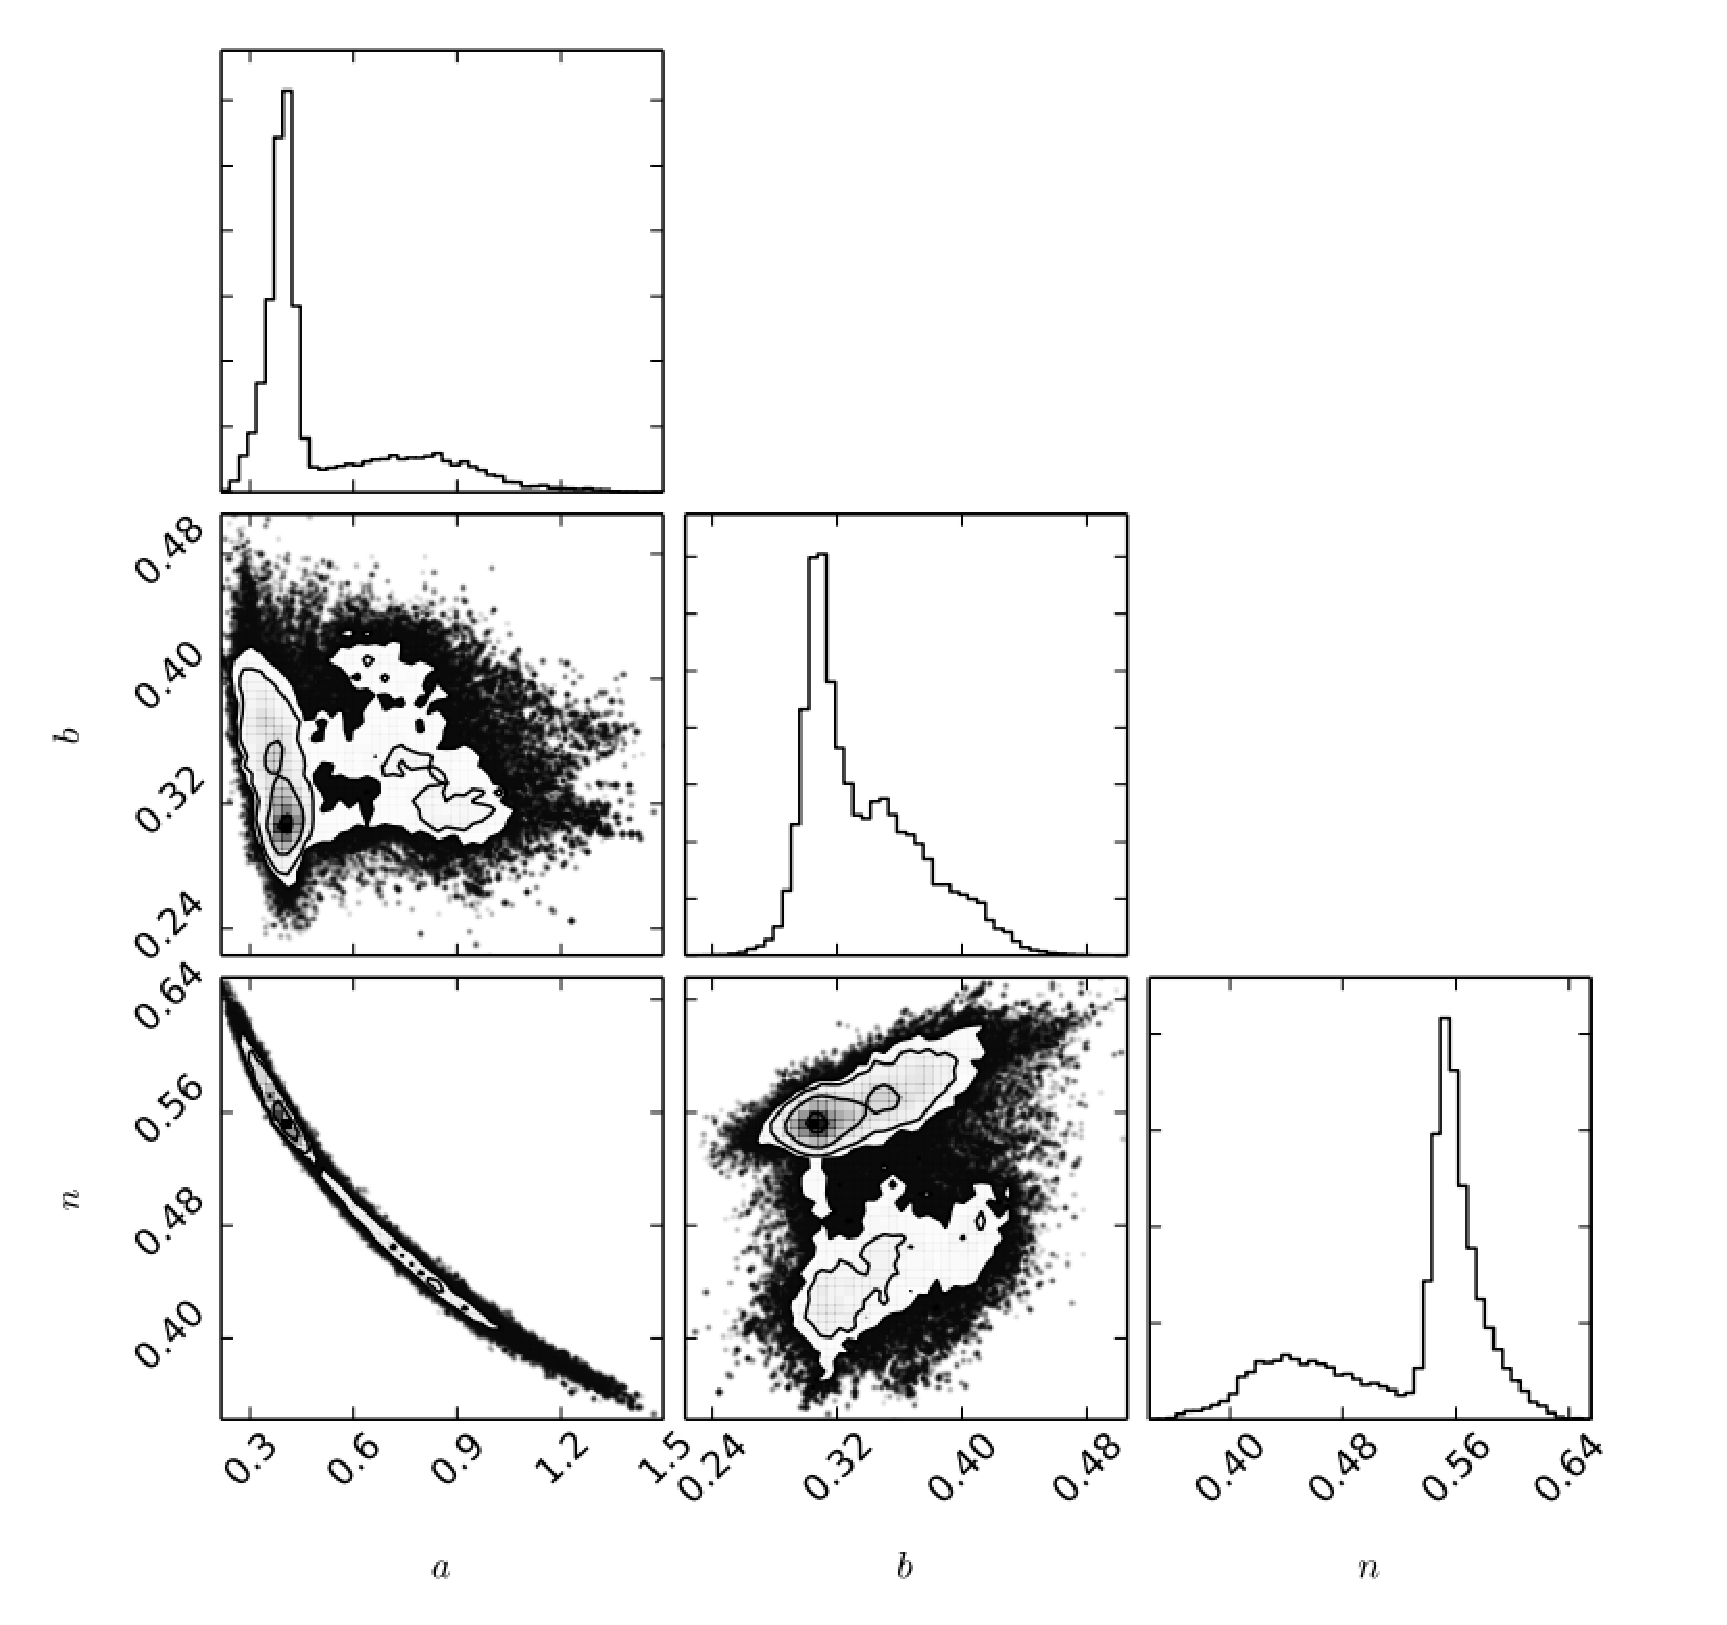
\includegraphics[width=6in, clip=false, trim=0 0 0.5in 0]{figures/small_triangleACHF.pdf}
\caption[Marginal posteriors of gyrochronology parameters]
{Marginalised posterior PDFs for the three gyrochronology
parameters, $a$, $b$ and $n$.
Parameters $a$ and $n$ are highly correlated and their
posterior PDFs are bimodal. The main peaks in the posterior PDFs of $a$ and
$n$ correspond to a fit to the Sun and field stars. The smaller peak
corresponds to a fit to the {\it Kepler} asteroseismic stars.
This plot was made using triangle.py
\citep{Corner}.
\label{fig:gyro_triangle}}
\end{center}
\end{figure*}

\begin{figure*}
\begin{center}
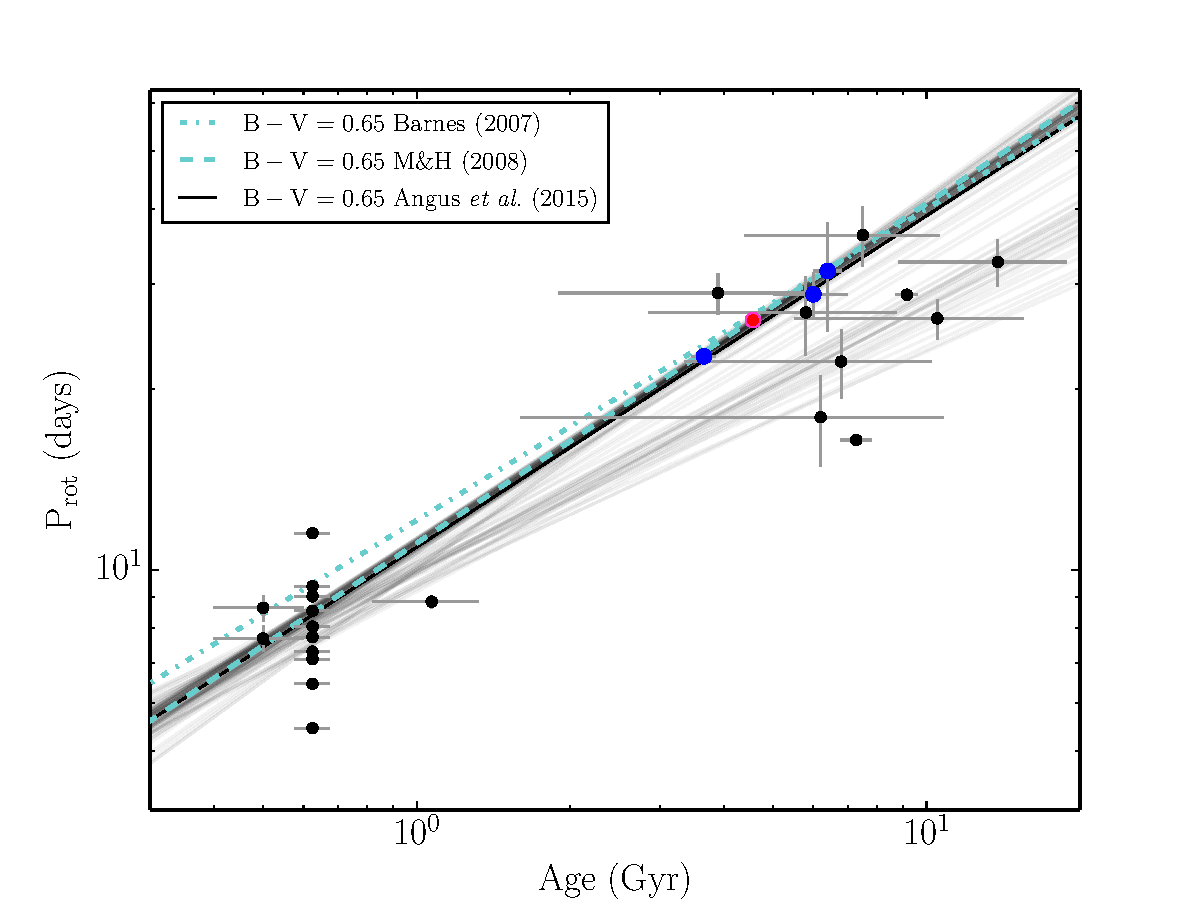
\includegraphics[width=6in, clip=true, trim=0 0 0.5in 0]{figures/p_vs_a_solar.pdf}
\caption[A new gyrochronology relation: period vs age.]
{Rotation period vs age for cool dwarfs with colour within 0.1 of the
	Sun's: 0.65, with gyrochronology relations of \citet{Barnes2007},
	\citet{Mamajek2008} and this work.
	The Sun is shown in red and the
	field stars, $\alpha$ Cen A, 18 Sco and 16 Cyg B from left to right,
	are shown in blue.
	The black points towards the lower left are cluster stars and those
	towards the upper right are {\it Kepler} asteroseismic stars.
	Each of the faint grey lines represents a
	sample drawn from the posterior probability distributions of $a$, $b$
	and $n$.
	Whilst most of these draws come from the large peak in the posterior
	PDF and fall through the Sun and field stars, some describe the
	period-age relation of the {\it Kepler} asteroseismic stars.
	These lines are drawn from the smaller peak in the posterior PDF.
\label{fig:p_vs_a_solar}}
\end{center}
\end{figure*}

\begin{figure*}
\begin{center}
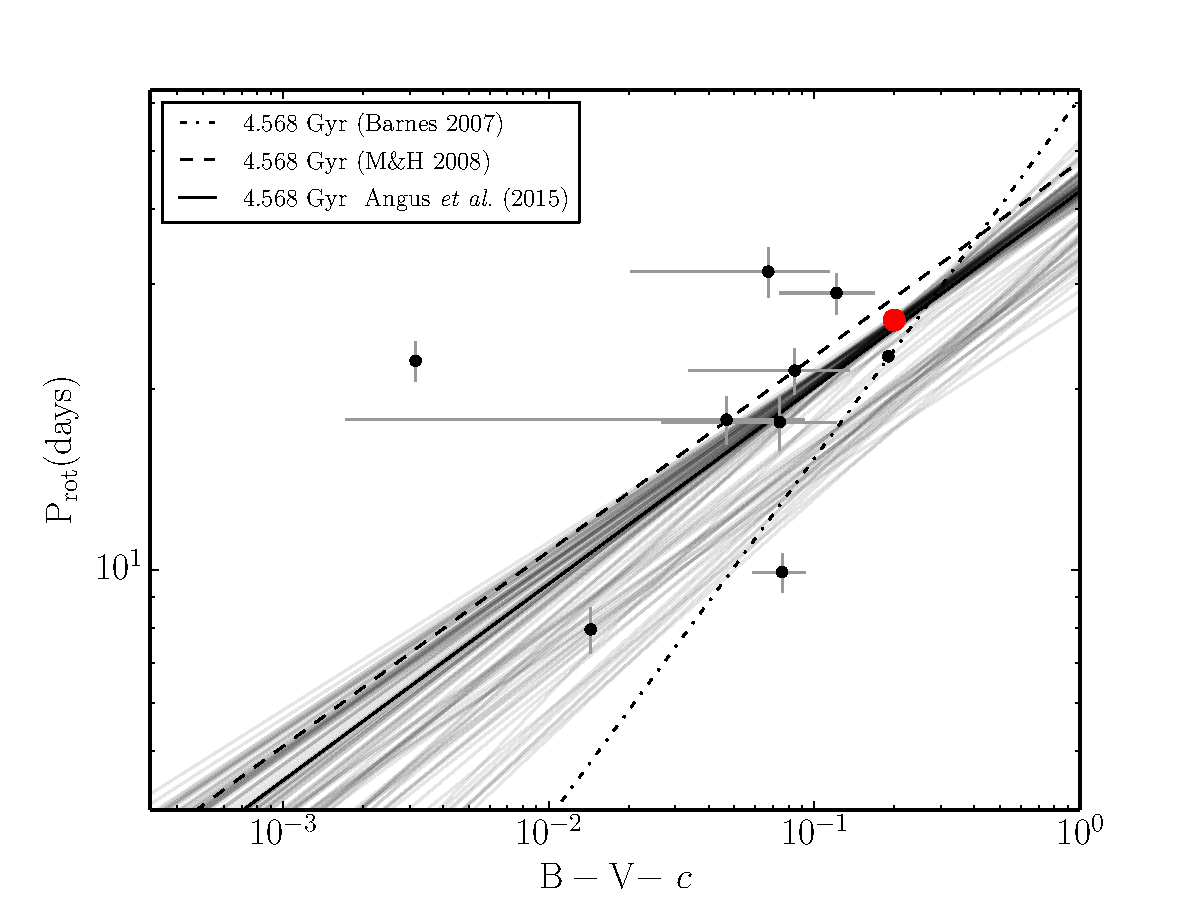
\includegraphics[width=6in, clip=true, trim=0 0 0.5in 0]{figures/p_vs_bv_solar.pdf}
\caption[A new gyrochronology relation: period vs colour.]
{Rotation period vs `$B-V-c$' for dwarfs with age within 1$\sigma$ of
	the Sun's age, 4.568 Gyr.
	The Sun is the red point.
	Each of the faint grey lines represents a
	sample drawn from the posterior probability distributions of $a$, $b$ and $n$.
	Many samples fall below the solid black line marking the highest
	probability parameter values due to the bimodal posterior.
\label{fig:p_vs_bv_solar}}
\end{center}
\end{figure*}

\begin{figure*}
\begin{center}
	\subfigure[0.5 Gyr (age of the Coma Ber)]{
            \label{fig:gyro_5}
	    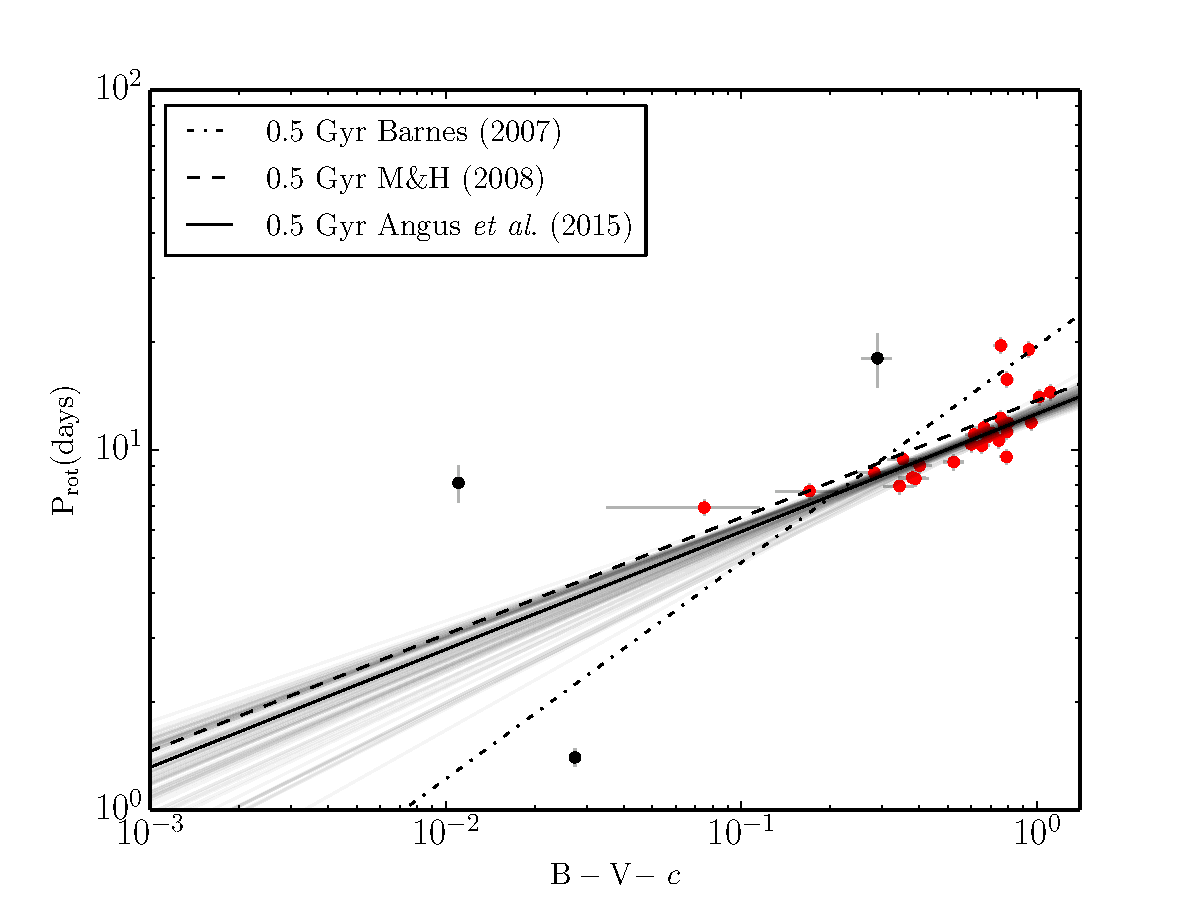
\includegraphics[width=2in]{figures/p_vs_bv0.pdf}
        }
	\subfigure[0.625 Gyr (age of the Hyades)]{
            \label{fig:625}
	    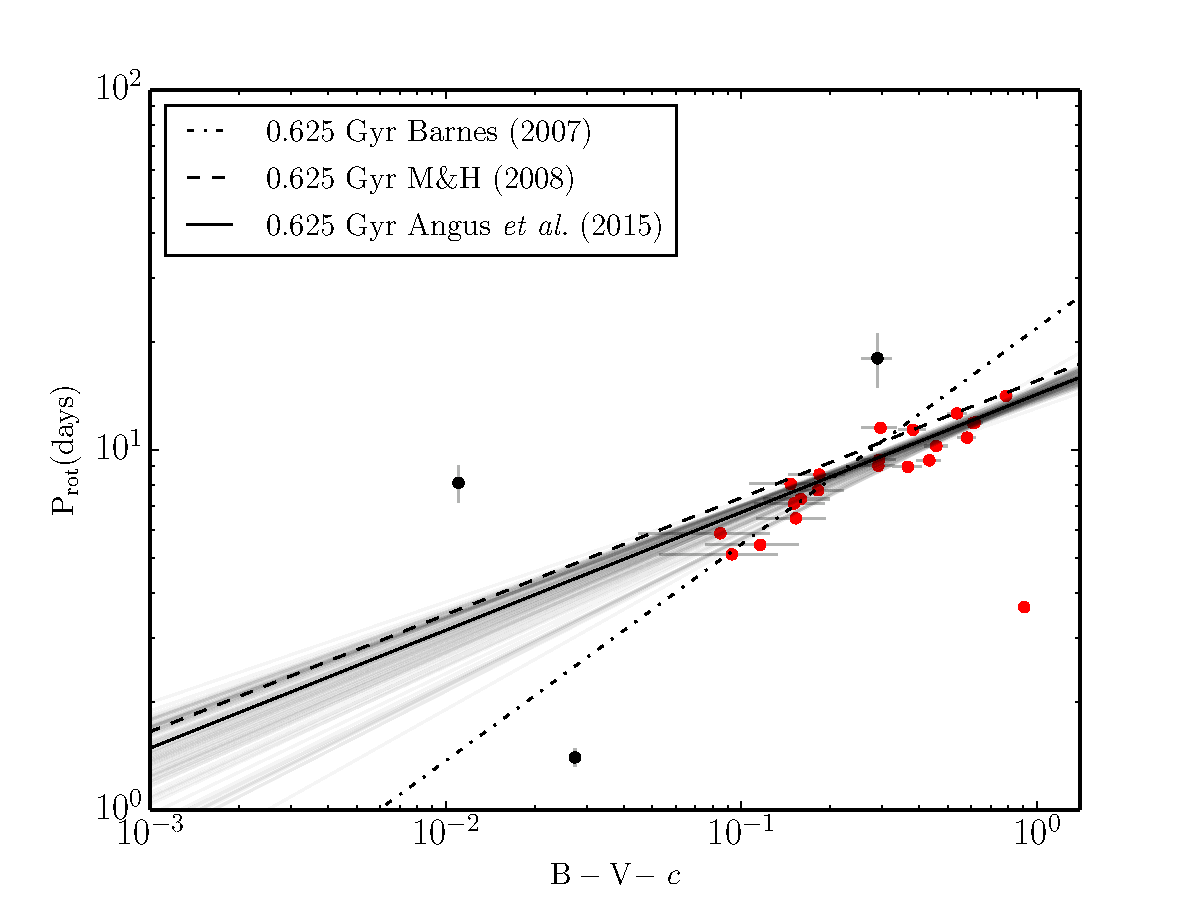
\includegraphics[width=2in]{figures/p_vs_bv1.pdf}
        }
	\subfigure[2 Gyr]{
            \label{fig:2gyr}
	    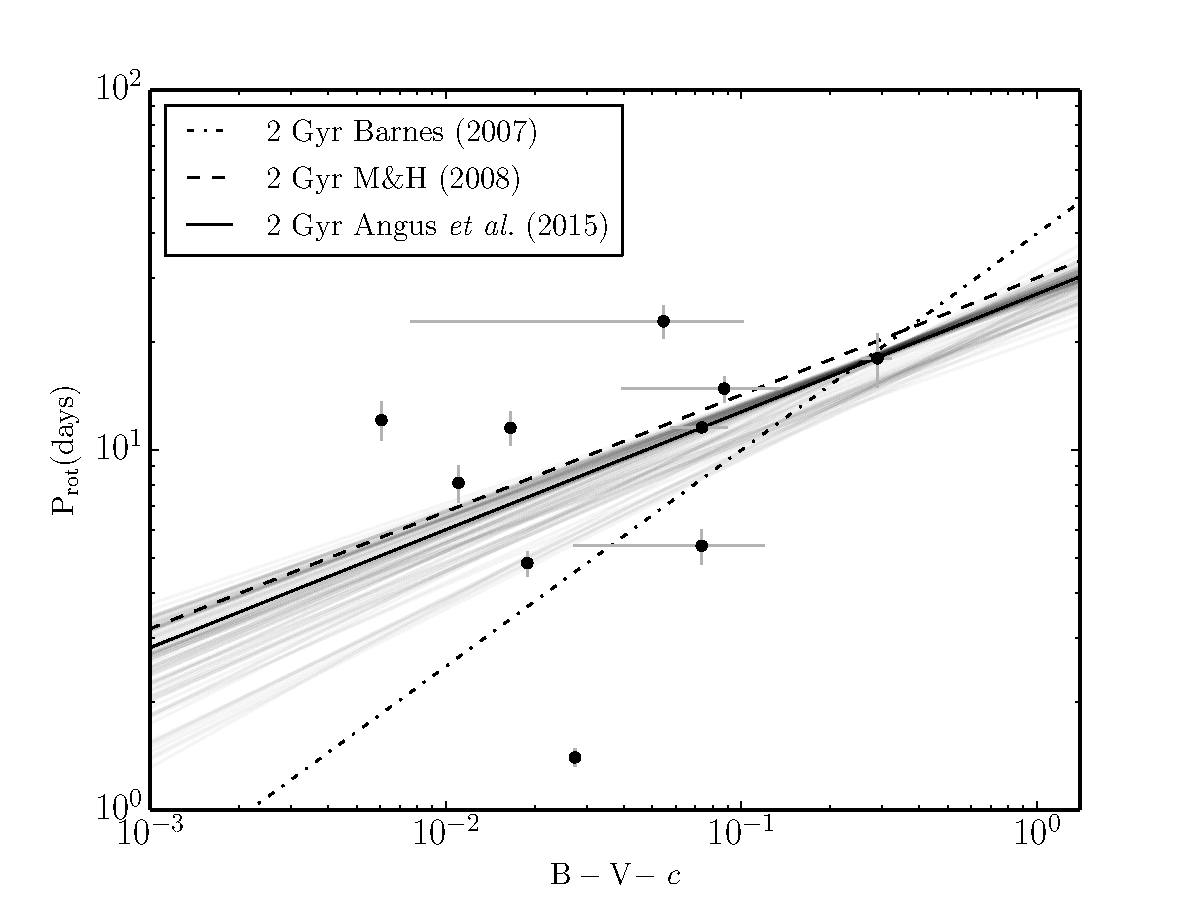
\includegraphics[width=2in]{figures/p_vs_bv2.pdf}
        }
	\subfigure[5 Gyr]{
            \label{fig:sungyr}
	    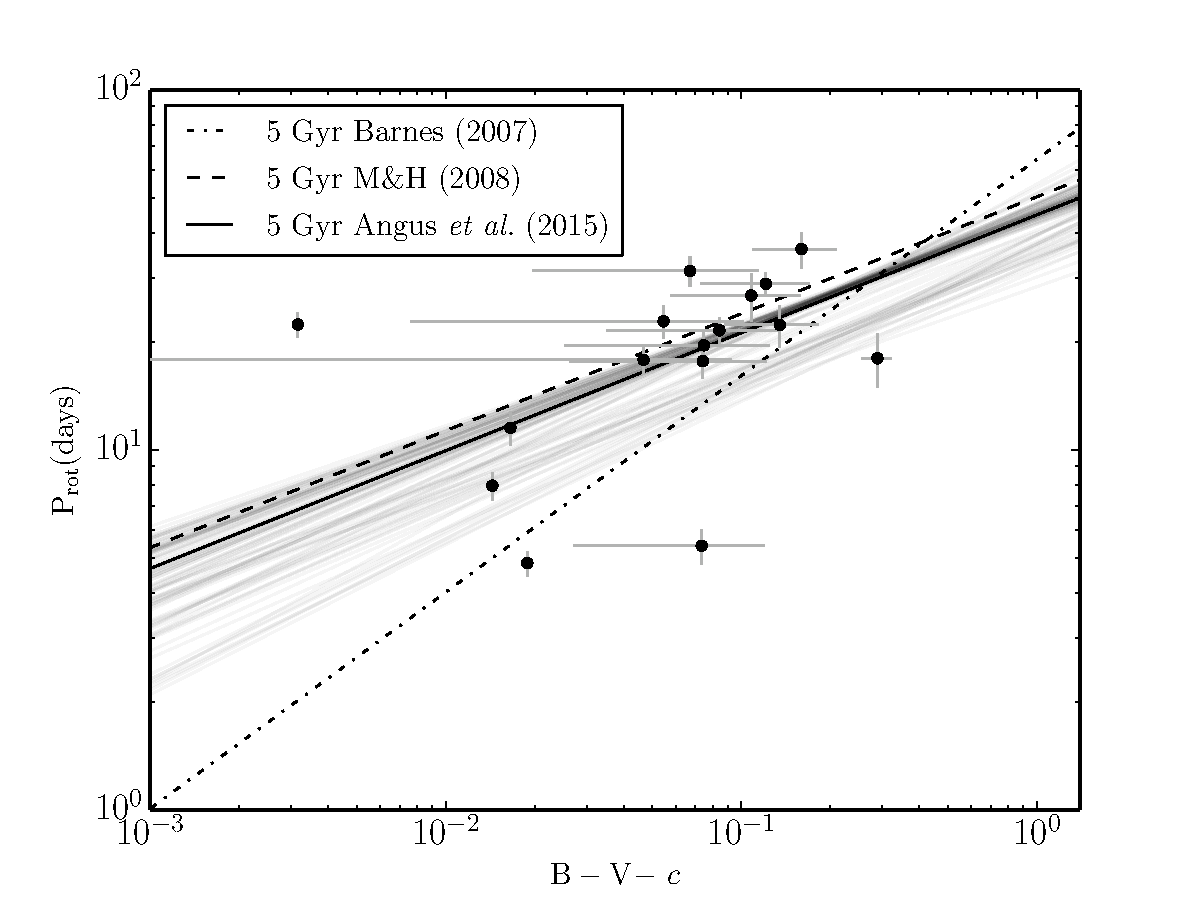
\includegraphics[width=2in]{figures/p_vs_bv3.pdf}
        }
	\subfigure[8 Gyr]{
            \label{fig:8gyr}
	    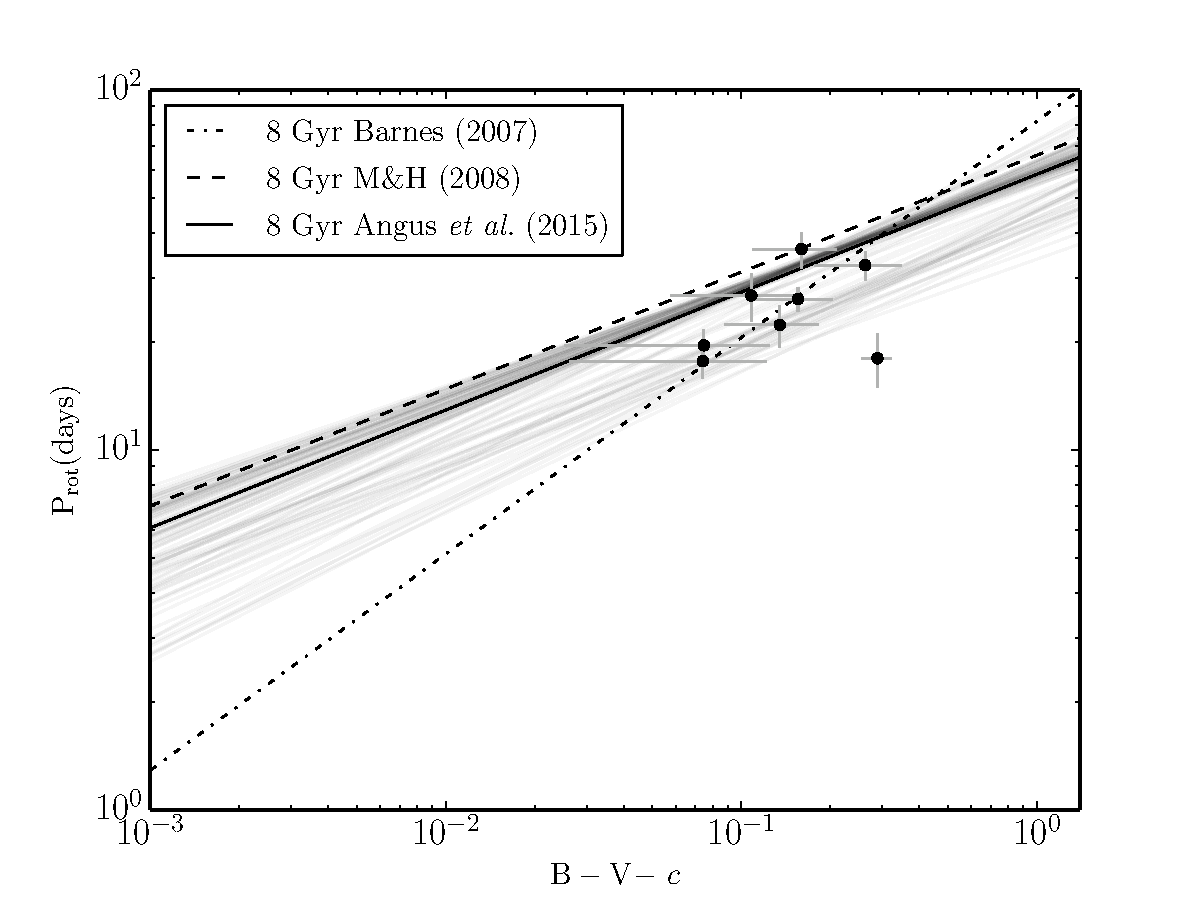
\includegraphics[width=2in]{figures/p_vs_bv4.pdf}
        }
    \end{center}
    \caption[Period vs colour over a range of ages]
{ \prot vs $B-V-c$ for dwarfs within 1$\sigma$ of the
reference age with the new gyrochronology relation and \citet{Barnes2007}, and
\citet{Mamajek2008} for comparison.
Asteroseismic targets are black and
cluster and field stars are red.
Each of the faint grey lines represents a
sample drawn from the posterior probability PDFs of $a$, $b$ and $n$.
Many samples fall below the best fit model due to the bimodal posterior PDFs.
\label{fig:subfigures2}}
\end{figure*}

Figure \ref{fig:gyro_triangle} shows that parameters $a$ and $n$ are
highly correlated and their posterior PDFs are bimodal.
The position of the second peak falls around $a = 0.8$, $b = 0.34$ and
$n = 0.44$.
The cause of this bimodality is clear when looking at the faint grey lines
representing draws from the parameter posterior PDFs in
figure \ref{fig:p_vs_a_solar}.
The majority of these draws fall close to the best-fitting model, which passes
neatly through the Sun and field stars, but a significant fraction fall
below the line of best-fit, passing through the {\it Kepler} asteroseismic
stars which also mostly fall below the line.
This result is reflected in \citet{Garcia2014} who model the AMP {\it Kepler}
asteroseismic stars from \citet{Mathur2012} and \citet{Metcalfe2014}, without
anchoring their relation to the Sun.
They find that the model that best describes the {\it Kepler} asteroseismic
stars underpredicts the rotation period of the Sun.
The grey lines that fall beneath our best-fitting model in figure
\ref{fig:p_vs_a_solar} are drawn from the smaller peak in the posterior PDFs
of $a$ and $n$ and seem to describe the relation between rotation period and
age for the {\it Kepler} asteroseismic stars.
In other words, the bimodal posterior PDFs of $a$ and $n$ are produced by the
disagreement between the {\it Kepler} asteroseismic stars and the Sun and field
stars.
% Although mostly consistent with this model they are not well
% described by it when taken in isolation.
One set of gyrochronology parameters is not
capable of describing the Sun, plus field stars, and the {\it Kepler}
asteroseismic stars simultaneously.
There is more than one possible explanation for this result.
Firstly, the asteroseismic ages could be systematically biased high.
% which could potentially result from the fact that the Kepler stars do
% not have well constrained metallicities.
Secondly, the rotation periods could be systematically underestimated.
This could occur if, for example, these stars were rotating differentially
and the dominant spotted regions on their surfaces were not equatorial, as is
the case for the Sun.
Thirdly, this could be a result of an observational bias produced by incomplete
detection.
If there were a large spread in rotation periods for a given stellar mass and
age and, due to the detection bias brought about because shorter periods are
easier to detect than longer periods, this broad range of rotation periods
might be truncated at some upper cut-off.
It would therefore appear as though Solar-colour stars were rotating too
slowly for their age simply because only rapidly rotating {\it Kepler} stars
appeared in our sample.
{\it Kepler} systematics hinder our ability to measure longer rotation periods,
but in addition, more slowly rotating stars tend to be less active, with
fewer surface features and are therefore more likely to be missing from our
sample.
Finally, it is possible that the {\it Kepler} asteroseismic stars follow a
\emph{different} spin-down relation to the Sun and field stars, perhaps due to
having different metallicities. % not referee
Unfortunately it is not currently possible to identify the cause of the
observed mismatch between the {\it Kepler} stars and the field stars and we leave
this question for a future investigation.
The tight correlation between parameters $a$ and $n$ demonstrates that there
is some redundancy in the fiducial gyrochronology relation.
In the future, an alternative functional form with less correlation between
parameters (for example a Gaussian process) should be explored.

The fact that our fit is so heavily dominated by the Sun with its small
uncertainties is, perhaps, a cause for concern.
We know the rotation period and age of the Sun very precisely, however, if the
Sun is not \emph{exactly} representative of a typical star, the resulting
best-fit gyrochronology relation will also not represent typical stars.
The field stars in our sample \emph{are} well represented by the best-fit
gyrochronology relation, which provides reassurance that the Sun is a typical
star amongst this set.
We did not attempt to tackle the problem of how to appropriately treat the Sun
as a single, highly-precise data point in a sample that also contains imprecise
data.
Instead, we leave this problem for future consideration.
Despite the fact that a lot of weight is attributed to the Sun because of its
small uncertainties, this new gyrochronology relation is still the most
representative, empirically calibrated relation between colour, rotation period
and age for MS F, G and K stars to date. % not referee

Our final, newly calibrated gyrochronology relation can be written in full as
\begin{equation}
	P = A^{\gyron^{+\nerrp}_{-\nerrm}} \times \gyroa^{+\aerrp}_{-\aerrm}
	(B-V-0.45)^{\gyrob^{+\berrp}_{-\berrm}},
\label{eq:Barnes2007_3}
\end{equation}
with rotation period, $P$ in days and age, $A$ in Myr.
An age can be calculated for a star with a rotation period and colour by
inverting this relationship.
Covariances between the gyrochronology parameters should
be taken into account {\it whenever} the above relation is used to calculate
uncertainties on an age or rotation period prediction.
In order to do this properly, posterior PDF samples should be incorporated
into Monte-Carlo uncertainty calculations\footnote{Posterior samples for
this project are available at https://github.com/RuthAngus/Gyro.}.

In order to test the predictive power of the new gyrochronology relation, we
inverted equation \ref{eq:Barnes2007_3} to compare previously measured ages
with new age predictions for the 6 field stars (see table
\ref{tab:comparison}).
For comparison, gyrochronological ages for the field stars were also computed
using the relations of \citet{Barnes2007} and \citet{Mamajek2008}.
Uncertainties on ages predicted with the new relation were calculated using
posterior PDF samples of the three parameters, $a$, $b$ and $n$.

\begin{table*}
\caption[Field star predictions]
{Field star ages taken from the literature, compared with
	predictions from this work (1), \citet{Mamajek2008} (2)
	and \citet{Barnes2007} (3). \label{tab:comparison}}

\begin{tabular}{lcccc}
\hline\hline
{Star} & {Literature age (Gyr)} & {Age 1 (Gyr)} & {Age 2 (Gyr)} & {Age 3 (Gyr)} \\
\hline

% age =  3.7146157634 2.47615796951 0.289790245663
18 Sco      & $3.7 \pm 0.2$     & $3.7^{+2.5}_{-0.3}$ & $3.5^{+0.6}_{-0.5}$
	    & $3.7^{+0.8}_{-0.6}$ \\

% age =  4.64289928616 3.52989315737 0.261371271108
The Sun     & $4.568 \pm 0.001$ & $4.6^{+3.5}_{-0.3}$ & $4.7^{+0.7}_{-0.6}$
	    & $4.8^{+1}_{-0.8}$ \\

% age =  5.01578686932 3.3247326735 1.01874883049
Alpha Cen A & $6.0 \pm 1$       & $5.0^{+3.3}_{-1.0}$   & $4.5^{+1}_{-0.9}$
	    & $5\pm1$ \\

% age =  6.03231609611 3.75246302579 1.67336060146
Alpha Cen B & $6.0 \pm 1$       & $6.0^{+3.8}_{-1.7}$       & $4^{+1}_{-0.9}$
	    & $5^{+2}_{-1}$ \\

% age =  4.04632196758 2.56486690245 0.691521414131
16 Cyg A    & $6.8 \pm 0.4$     & $4.0^{+2.6}_{-0.7}$       & $3\pm2$
	    & $4\pm2$ \\

% age =  3.65467896474 3.36668380102 2.12516472969
16 Cyg B    & $6.8 \pm 0.4$     & $3.7^{+3.4}_{-2.1}$       & $3\pm2$
	    & $4\pm2$ \\
\hline
\end{tabular}
\end{table*}

The ages predicted by the three different relations are consistent within
uncertainties, with the exception of Alpha Cen B.
All three relations underpredict the age of the 16 Cyg system.
The rotation periods of both 16 Cyg A and B used in this paper are
asteroseismic measurements of the internal (not surface) rotation periods
of the stars.
If the stars' cores are rotating much more rapidly than their surfaces, this
could account for this age discrepancy.

The goal of gyrochronology in general is to provide a means of predicting the
age of a star given observations of its colour (or mass, or temperature), and
rotation period.
The discrepancies in period-colour relations between clusters, {\it Kepler}
stars and nearby field stars in the above analysis does not bode well for the
current, simple gyrochronology model.
Although the individual gyrochronology ages predicted for most of the \kepler\
stars lie within the errobars of the asteroseismic ages, there is an
unmistakable systematic offset which cannot be described by the model.
Until now it has been hoped that one single relation between period, mass and
age could be used to describe all F, G and K MS stars.
Even though we are unable to identify the cause of the discrepancy between the
{\it Kepler} stars and the field stars, a different gyrochronology relation
still seems to be required for each cluster.
This may simply be due to a metallicity discrepancy, but this still
demonstrates that the simple gyrochronology relation used here is inadequate.

The `narrowness' of the gyrochronology relation has hitherto been an unknown;
do the three properties, age, mass and rotation period, truly lie on an
infinitely narrow plane?
Unfortunately we cannot fully answer this question here as the asteroseismic
ages are noisy and observational and intrinsic scatter are ambiguously
interwoven.
However, if this sample of stars is subject to detection bias then, by
definition, there must be a broad range of rotation periods for stars of a
given mass and age.
A future study might include an extra parameter that describes the `width' of
the gyrochronological plane and attempt to detect an element of scatter above
the noise level.
Does age depend solely on rotation period and mass or do other variables
influence stellar spin down, perhaps only becoming important after many Myrs?
The gyrochronology model calibrated here neglects the effects of metallicity.
This property is bound to have an effect on the angular momentum evolution
of a star since it impacts internal stellar structure.
A future study, investigating the impact of metallicity on rotational evolution
will be essential for improving our ability to date stars using gyrochronology.

The picture of gyrochronology will become clearer as the sample of
asteroseismic stars with individual mode analysis grows and their age
uncertainties shrink.
The best targets for asteroseismic studies are relatively inactive since they
allow the easier detection of Solar-like oscillations.
Inactive stars are also the best targets for gyrochronology as they are
usually old and slowly rotating.
However these targets are not well suited for
rotation period measurements which are most easily and precisely determined
for active, rapidly rotating stars.
K2, the repurposed {\it Kepler} mission, will provide new targets for rotation
studies; in particular, some relatively old clusters have been and will
continue to be monitored by the spacecraft.
The observing seasons of K2 are relatively short ($\sim$ 90 days) and fields
will only be observed once, so the maximum rotation periods measurable from
K2 light curves will be considerably shorter than with {\it Kepler}.
However these clusters may still be extremely useful for gyrochronology.

\section{Conclusions}
\label{sec:conclusions}

We have calibrated the relation between rotation period, $B-V$ colour and age
for MS stars with \teff$<$ 6250 K, using \nastero$~${\it Kepler} asteroseismic
targets, supplemented with 6 field stars and \nHC$~$cluster stars.
Unlike previous gyrochronology calibrations, our sample covers a large range
of ages, observational uncertainties on all parameters were accounted for and
the posterior PDFs of model parameters were explored using MCMC.
Incorporating observational uncertainties into the model fitting process was
an essential component of our analysis since these uncertainties, particularly
on the asteroseismic ages, were large.
Three populations: hot dwarfs, cool dwarfs and subgiants, were modelled
simultaneously in order to account for potential misclassifications that
might have arisen from large observational uncertainties.
Posterior probability distributions of the gyrochronology parameters were
explored using MCMC and the impact of leaving out subsets of the sample was
assessed, leading us to find that a single relation between rotation period,
colour and age does not adequately describe the cluster data.
For this reason, only the Hyades and Coma Berenices clusters were used to
calibrate the model.
Fitting equation \ref{eq:Barnes2007_2} to the Hyades and Coma Berenices
clusters, the {\it Kepler} asteroseismic stars, local field stars and the Sun
resulted in bimodal posterior PDFs.
The {\it Kepler} asteroseismic stars were not well described by the same
gyrochronology relation as the Sun, field stars and clusters.
There are several potential explanations for the cause of this phenomenon.
Some of the most likely are: the asteroseismic ages or the photometric
rotation periods could be systematically biased; the rotation periods might be
subject to detection bias; and the different
populations could have different physical properties (e.g. metallicity), not
accounted for in the gyrochronology model.
If detection bias is responsible and there truely {\it is} a broad range of
rotation periods for stars of a given age and colour, this still has
negative implications for Gyrochronology which relies on the assumption that
these three properties lie on a neat plane.


The careful and well motivated modelling techniques used in this work
allowed us to identify the potential shortcomings of the current
gyrochronology model.
Only by conducting MCMC parameter exploration and studying the resulting
posterior PDFs were we able to see that one global gyrochronology relation
cannot describe all subsets of our sample.
The results are somewhat unsettling---no single model describes the sample as
a whole, even when dropping some of the clusters and allowing for rather
complex population subsets.
This tells us that the current model is probably not good enough, but it - or
something very similar - is the model everyone has been using in
gyrochronology studies so far.
Previous studies did not model multiple cluster and field populations
simultaneously, or do the modelling in such a detailed way, so the problems
did not come through so clearly.
In the future better physical models may be developed, better ages may be
calculated and more sensitive period search methods, not so susceptible to
detection bias may become available.
When they do, the prescription we provide will enable the the
period-colour-age relation to be modelled more sensitively.

Since the work in this chapter was published \citep{Angus2015}, the
result seen here: that \kepler\ asteroseismic stars rotate unexpectedly
rapidly given their age and mass, was also found by \citet{Vansaders2016}.
Instead of using the entire ensemble of short cadence asteroseismic targets
from \citet{Chaplin2014}, they used only `boutique' targets.
These are the highest S/N stars with individual oscillation mode frequencies
detectable in their power spectra.
These targets are also not well described by existing gyrochronology
models.
Whereas I showed that the \citet{Barnes2007} empirical form did not
fit the data, \citet{Vansaders2016} compare rotation periods to predictions
made using their theoretically motivated model, equation \ref{eq:vansaders} in
chapter \ref{chapter:intro}.
They cannot reproduce the observations using their model and present the
following alteration which {\it does} describe the data:
\begin{equation}
\frac{dJ}{dt} = \left\{
                \begin{array}{ll}
                  f_K K_M \omega \left( \frac{\omega_{crit}}{\omega_\odot}
                  \right)^2, \omega_{crit} \leq \omega
                  \frac{\tau_{c}}{\tau_{c, \odot}}, Ro \leq Ro_{crit} \\
                  f_K K_M \omega \left( \frac{\omega\tau_{c}}
                  {\omega_\odot\tau_{c, \odot}}
                  \right)^2, \omega_{crit} > \omega
                  \frac{\tau_{c}}{\tau_{c, \odot}}, Ro \leq Ro_{crit} \\
                  0, Ro > Ro_{crit}
                \end{array}
              \right.,
\end{equation}
where $K_M$ is defined in equation \ref{eq:vansaders2}.
By introducing a threshold Rossby number, $Ro_{crit}$, above which there is
no angular braking, they are able to reproduce the observations.
By fitting their model to the \kepler\ targets and the Sun they find
$Ro_{crit} = Ro_\odot = 2.16$.

In order to test this theory it is imperative that we obtain new
observations---in particular, rotation periods of old stars with precise and
reliable ages.
\LSST\ may provide rotation periods for old field stars (see chapter
\ref{chapter:future}.
In the interim, \ktwo\ is observing several open clusters that will add to our
arsenal of precisely dated stars with rotation periods, provided we can
extract rotation period signals from \ktwo's noisy light curves.

% acknowledgements
% The code used in this project can be found at
% https://github.com/RuthAngus/Gyro.
% R.A. acknowledges funding from the Leverhulme Trust.
% A.M. acknowledges funding from the European Research Council under the EU’s
% Seventh Framework Programme (FP7/(2007-2013)/ERC Grant Agreement No. 291352).
% We wish to thank the anonymous referee for their valuable and insightful
% feedback and Bill Chaplin for his thoughtful and detailed comments
% which enormously improved this paper.
% We would also like to thank Tsevi Maseh, Eric Mamajek, Daniel Mortlock and
% David Hogg for useful insight and discussion that hugely contributed to this
% paper.

% \bibliographystyle{mn2e}
% \bibliography{Gyro_paper}

% \end{document}

\chapter{Systematics-insensitive periodic signal search with K2}
\label{chapter:sip}

\begin{abstract}

% Aims
From pulsating stars to transiting exoplanets, the search for periodic signals
in {\it K2} data, {\it Kepler's} 2-wheeled extension, is relevant to a long
list of scientific goals.
Systematics affecting {\it K2} light curves due to the decreased
spacecraft pointing precision inhibit the easy extraction of periodic signals
from the data.
We here develop a method for producing periodograms of K2 light curves that
are insensitive to pointing-induced systematics; the Systematics-Insensitive
Periodogram (SIP).
% Methods
Traditional sine-fitting periodograms use a generative model to find the
frequency of a sinusoid that best describes the data.
We extend this principle by including systematic trends, based on a set of
`Eigen light curves', following \citet{Foreman-Mackey2015}, in our generative
model as well as a sum of sine and cosine functions over a grid of
frequencies.
% Results
Using this method we are able to produce periodograms with vastly reduced
systematic features.
The quality of the resulting periodograms are such that we can recover
acoustic oscillations in giant stars and measure stellar rotation periods
without the need for any detrending.
The algorithm is also applicable to the detection of other periodic phenomena
such as variable stars, eclipsing binaries and short-period exoplanet
candidates.
The SIP code is available at \url{https://github.com/RuthAngus/SIPK2}.

\end{abstract}

\section{Introduction}
\label{Introduction}

The excellent precision achieved by the original {\it Kepler} mission relied
on extremely precise pointing, for which three reaction wheels were required.
% John: cite original mission and Howell here.
After the failure of one of these wheels, the {\it Kepler} team devised a new
pointing scheme in which the spacecraft is stabilized by the Solar wind for
ecliptic plane viewing zones \citep{Howell2014}.
In this configuration the spacecraft is able to maintain an unstable
equilibrium, with the two functioning reaction wheels controlling pitch and
yaw whilst the spacecraft slowly rolls about the boresight.
The spacecraft fires its thrusters once every $\sim$ 6 hours
\citep[][hereafter VJ14]{Vanderburg2014} to correct for
this slow drift and, as stars move across pixels with different sensitivities,
their flux varies.
The extraction of high-precision photometry from {\it K2} target pixel files,
despite the reduced pointing precision, is a requirement for many fields of
research and several methods for the extraction and detrending of {\it K2}
light curves have already been developed.
For example, VJ14 and \citet{Crossfield2015}
use simple aperture photometry and correct the light curve of each star
individually and \citet{Aigrain2015} use a Gaussian process to model the
non-linear dependence of stellar flux on the roll angle of the telescope.

\begin{figure}[p]
\begin{center}
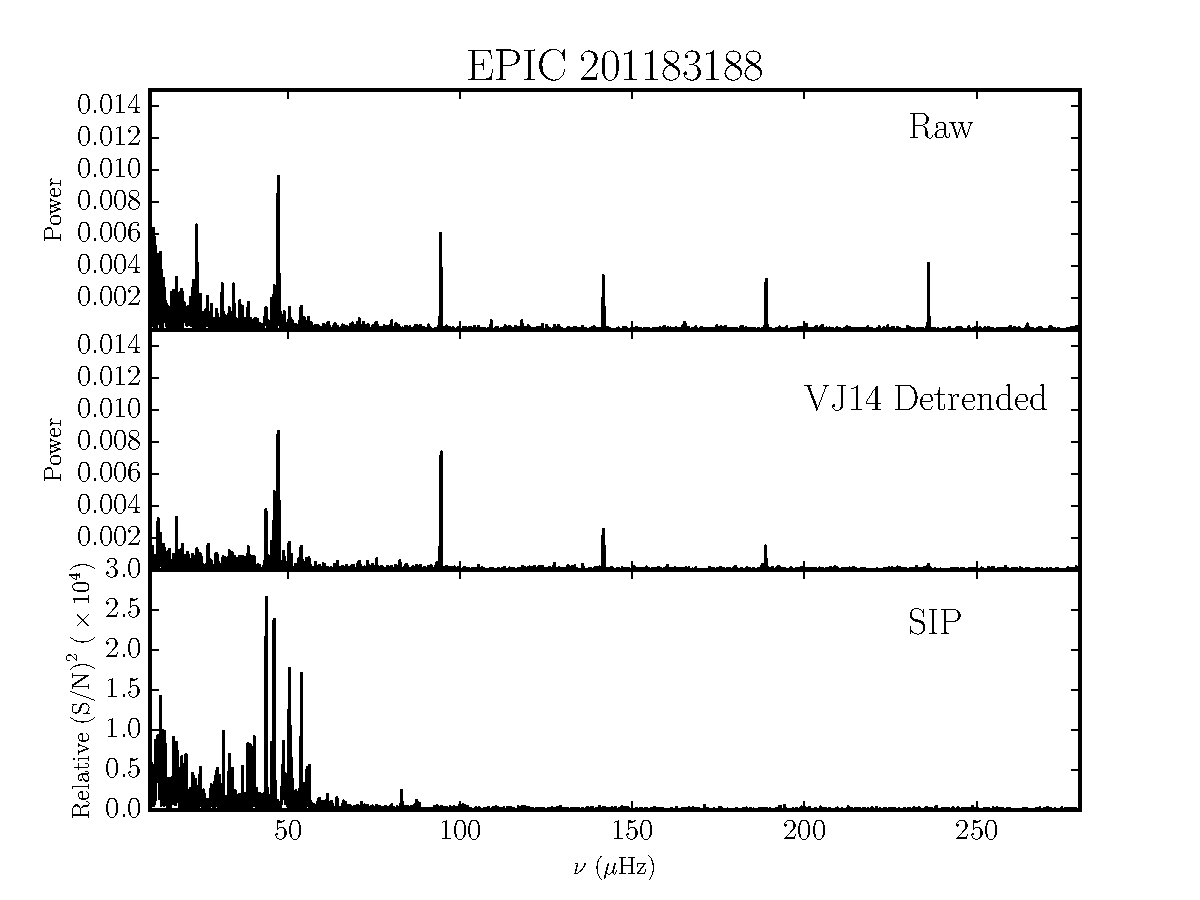
\includegraphics[width=6in, clip=true]{figures/rawvbg_201183188.pdf}
\caption[Comparing the SIP to a detrended LS periodogram.]
{LS periodograms of the raw (Top) and VJ14--detrended (middle) {\it K2}
	 light curves of EPIC 201183188.
	 The bottom panel shows the SIP for this target.
	 Peaks at $\sim$ 47 $\mu$Hz and its harmonics produced by the regular
	 spacecraft thruster fires are still present in the LS periodogram of
	 the detrended data, but do not appear in the SIP.}
\label{fig:raw}
\end{center}
\end{figure}

Whilst these methods successfully remove most systematic trends and
produce light curves suitable for exoplanet search and some stellar
variability studies, residual systematics can still affect the light curves on
timescales relevent to asteroseismology and stellar rotation.
In particular, the $\sim$ 6 hour thruster firing signal may still appear
with high power in the periodograms of these detrended light curves
(see figure \ref{fig:raw}).
A detrending method for {\it K2} light curves, specifically intended for the
asteroseismic analysis of giant stars has been developed by \citet{Lund2015},
in which the systematics due to roll are corrected, again on
a star-by-star basis and any remaining periodic signals at 47 $\mu$Hz (6 hour
period) or its harmonics are removed by prewhitening.
The method developed here, the Systematics-Insenstive Periodogram (SIP)
produces periodograms of {\it K2} light curves without the need for detrending
or prewhitening.

\subsection{Asteroseismology}

As well as providing data that have lead to the discovery thousands of
exoplanets, the original {\it Kepler} mission revolutionized many fields of
stellar astronomy, particularly asteroseismology.
Fundamental stellar parameters---in some cases, extremely precise ones---can
be calculated for {\it Kepler} asteroseismic stars from the power spectra of
their light curves.
Although Sun-like stars oscillate at high frequencies and require
short-cadence observations, pulsations of giant stars lie below the Nyquist
frequency set by the 28.5 minute sampling rate of long cadence {\it Kepler}
data: 283 $\mu$Hz.
Asteroseismic analysis of data from the original {\it Kepler} mission is
traditionally conducted upon detrended light curves.
For short cadence {\it Kepler} data, this detrending method is described in
\citet{Garcia2011}.
Due to the precise pointing of the original {\it Kepler} mission, systematics
present in these light curves, caused by temperature fluctuations and minor
pointing shifts, are relatively low amplitude.

However, this is not the case for {\it K2} light curves: the precision over a
6 hour timescale is estimated to be 4 times worse in {\it K2} data
\citep{Howell2014}, therefore new approaches to the treatment of systematics
are necessary.
Figure \ref{fig:raw} demonstrates the need for careful systematics treatment
of {\it K2} photometry for asteroseismology.
The top panel shows a Lomb-Scargle\footnote{All LS periodograms
produced in this project were produced using the gatspy Python module:
\url{https://github.com/astroML/gatspy/tree/master/gatspy/periodic}} (LS)
periodogram of the raw, simple aperture photometry\footnote{The method used to
extract this photometry is described in \textsection \ref{sec:Method}} of EPIC
201183188, a pulsating giant star.
The large peaks at $\sim$ 47 $\mu$Hz and its harmonics are caused by the
regular thruster fires of the spacecraft.
The bottom panel shows the LS periodogram of this light curve, after
it has been detrended using the method of VJ14.
The large peaks are still present in the detrended light curve.
The dominant source of these peaks is the removal of the outlying data points
that appear in the {\it K2} light curves every 6 hours, caused by the
spacecraft thruster fires.
The rapid motion of the spacecraft results in stellar flux being smeared out
over the detector and the circular apertures do not adequately encompass the
resulting point spread function.
It is the removal of these data points that produces the 47 $\mu$Hz peak in
the VJ14 periodogram.
While the noise source at 47 $\mu$Hz does not interfere with the detection of
high-signal-to-noise transit events for periods greater than $\sim$1 day
\citep{Vanderburg2015}, it does hamper the detection of
smaller signals, particularly on time scales comparable to that of thruster
fires.
These peaks lie in an important region of parameter space for giant star
asteroseismology and could affect the stellar parameters measured for thousands
of giants if not dealt with appropriately.

\subsection{Stellar rotation}

Stellar rotation studies have hugely benefitted from the era of high-precision
space photometry.
Active regions on the surface of rotating stars produce periodic variations
in flux and stellar rotation periods can therefore be measured from
{\it Kepler} light curves.
Stellar rotation is a field of active interest as the rotation period of star
can be used to infer its age via gyrochronology
\citep{Skumanich1972, Barnes2007, Epstein2014, Angus2015}, is thought to be
tied to the stellar magnetic dynamo, and could even reveal dynamical
interations with companion stars or planets
\citep[e.g.][]{Beky2014, Poppenhaeger2014}.
Current methods for measuring rotation periods from {\it Kepler} light curves
include periodogram \citep[e.g.][]{Reinhold2013}, AutoCorrelation Function
(ACF) \citep{Mcquillan2013} and wavelet \citep[e.g.][]{Garcia2014} analysis,
or some combination thereof.
Stellar variability is not typically sinusoidal, therefore sine-fitting
periodograms are not perfectly suited to measuring rotation periods
\citep{Mcquillan2013}.
For this reason, the ACF method is often favoured over the periodogram method.
However, because autocorrelation is performed directly on detrended light
curves, and cannot be written down as a generative model, it is not possible
use autocorrelation techniques on untreated {\it K2} data.
A quasi-periodic Gaussian process is a much better effective model for stellar
variability than a sinusoid, however we choose to focus on the more generally
applicable (and computationally tractable) sine-wave periodogram, leaving the
Gaussian process periodogram for future consideration.

In this \article\ we focus on the examples of asteroseismology and stellar
rotation, however many other fields of astronomy utilize periodic information
in {\it K2} light curves.
These include studies of eclipsing binaries, variable stars, exoplanets, white
dwarfs and even AGN.
The development of tools for extracting periodic information from {\it K2}
data is essential if it is to be as revolutionary in time-domain
astronomy as the original {\it Kepler} mission was.

In \textsection\ref{sec:Method} we outline the method behind the SIP.
In \textsection\ref{section:rotation} we apply the SIP to real {\it K2} light
curves, using some giant asteroseismic pulsators and rotating stars as test
cases and then provide the results of some simple tests which show exactly
{\it how} `insensitive' the SIP is to systematic features.
Finally, we demonstrate the SIP's usefulness regarding other periodically
varying objects in this section, before presenting our conclusions in
\textsection\ref{sec:conclusions}.

\section{Method}
\label{sec:Method}

The method implemented in this \article\ is an extention of the planet-search
algorithm developed by \citet{Foreman-Mackey2015} (hereafter FM15).
All targets observed by {\it Kepler} move on the CCD in the same way,
therefore the systematics affecting each individual star's light curve have
shared properties.
The FM15 method uses this fact by decomposing the light curves into a set
of `Eigen Light Curves' (ELCs) using Principle Component Analysis (PCA), which
can be used to model any individual star's light curve with very little loss
of information.
This process is similar to the method used to produce PDC-MAP data for the
original {\it Kepler} mission \citep[][]{Stumpe2012, Smith2012}.
The resulting ELCs from campaign 1 can be used to model any campaign 1 {\it
K2} light curve, (campaign 0 ELCs for campaign 0, etc) and specifically, can
model the data in combination with an arbitrary physical model.

In order to construct sets of ELCs for campaigns 0 and 1, FM15 downloaded the
target pixel files for all stars in these two fields.
% ; 21,703 in total.
The position of each star was predicted using the World Coordinate System (WCS)
and 10 circular apertures placed around the star with radii varying from 1 to
5 pixels in steps of 0.5 pixels.
Following the procedure of VJ14, the aperture producing the
light curve with the lowest CDPP within a 6 hour window
\citep{Christiansen2012} was selected\footnote{The simple aperture photometry
light curves for campaigns 0 and 1 are available at
\url{http://bbq.dfm.io/ketu/lightcurves/}}.
PCA was then performed on the full set of targets in order to produce ELCs.

FM15 used 150 of these ELCs, plus a transit model, in order to
search for exoplanet candidates without the need for a `detrending' step.
The likelihood of the data, conditioned on the ELC-plus-transit
model was calculated over a fine grid of periods and transit depths, resulting
in the detection of 36 new exoplanet candidates.
% We use exactly the same technique to find periodic signals in {\it K2} data,
% however, instead of an exoplanet transit, our model is a sinusoid.
We use a very similar technique to find periodic signals in K2 data.
The primary difference is that we use a sinusoid rather than a transit model.
This model is linear, therefore the likelihood function conditioned on
a specific frequency can be calculated and the systematics model marginalized
over analytically.

Following the notation in FM15, our model for the $k$th star can be written
\begin{equation}
	\mathbf{f_k} = \mathbf{A}\mathbf{w_k} + \mathrm{noise},
\end{equation}
where $\mathbf{f_k}$ is the vector of $N$ flux values,
\begin{equation}
	\mathbf{f_k} = (f_{k,1}, f_{k,2}, f_{k,3}, ..., f_{k,N})^T
\end{equation}
at times
\begin{equation}
	\mathbf{t_k} = (t_1, t_2, t_3, ..., t_N)^T.
\end{equation}
$\mathbf{A}$ is the design matrix:
\begin{eqnarray}
	\mathbf{A} &=& \left (\begin{array}{ccccccc}
	x_{1,1} & x_{2,1} & \cdots & x_{150,1} & 1 & \sin(2\pi\nu t_1) & \cos(2\pi\nu t_1) \\
	x_{1,2} & x_{2,2} & \cdots & x_{150,2} & 1 & \sin(2\pi\nu t_2) & \cos(2\pi\nu t_2\\
    && \vdots &&&\\
	x_{1,N} & x_{2,N} & \cdots & x_{150,N} & 1 & \sin(2\pi\nu t_N) & \cos(2\pi\nu t_N)
\end{array}\right )
\end{eqnarray}
where the $x_{ij}$s are the ELCs\footnote{Campaign 0 and 1 ELCs are
available at \url{http://bbq.dfm.io/ketu/elcs/}}, with $i$ denoting the ELC number
and $j$ the time index.
The design matrix contains the basis functions of the linear model.
The basis functions for the systematic features in the light curves are the ELC
values at each time index, the sine and cosine terms are the basis functions of
the sinusoidal signal of interest, and the `1's describe a linear offset.
Any {\it K2} light curve can be reproduced as a linear combination of these
basis functions.
We are interested in the last two elements of the weight vector: the
coefficients of the sinusoidal signal.
The maximum likelihood solution for the weight vector,
$\mathbf{w}$ is
\begin{equation}
	\mathbf{w_k}^* \gets (\mathbf{A}^T\mathbf{A})^{-1}\mathbf{A}^T\mathbf{f_k}.
\end{equation}

Under this linear model with Gaussian uncertainties, the marginalized
likelihood for the periodic amplitude is a two-dimensional Gaussian with mean
given by the last two elements ($\mathbf{a}$) of $\mathbf{w}*$ and covariance
given by the bottom right two-by-two block ($\mathbf{S_a}$) of
$(\mathbf{A}^T \mathbf{C}^{-1} \mathbf{A})^{-1}$, where the $\mathbf{C}$
matrix contains observational uncertainties on the diagonal.
These uncertainties are estimated as $1.48 \times$ the Median Absolute
Deviation (MAD), following \citet{Aigrain2015}.
Therefore, the signal-to-noise ratio, $S/N$ of the amplitude measurement is
$\sqrt{\mathbf{a}^T \mathbf{S_a}^{-1} \mathbf{a}}$.
The $(S/N)^2$ can then be calculated over a user-defined grid of frequencies
to produce a SIP.
The $(S/N)$ operation takes into account the goodness of fit, i.e. if the
amplitude of the sinusoid at a given frequency is not well constrained,
it is penalized.
The SIP algorithm scales linearly with the number of frequencies evaluated
and with the cube of the number of basis functions used.
As an example of the typical computation time, calculating a single SIP for a
{\it K2} campaign 1 light curve, over a grid of 1000 frequencies with 150
basis vectors, takes 2-3 seconds on a 2.7 GHz CPU.

\section{Application to real light curves}
\label{section:rotation}

An example LS periodogram of the raw {\it K2} photometry
for giant star, EPIC 201183188 is shown in figure \ref{fig:raw}.
Peaks appearing at 47 $\mu$Hz and its harmonics are produced by the regular
$\sim$ 6 hour thruster fires that repoint the spacecraft.
These peaks are also present in periodograms of the VJ14 detrended light
curves.
The presence of systematic signals at these timescales are problematic for
asteroseismic analysis since they lie in a region of frequency space
that is often populated by giant asteroseismic modes.
It is possible to remove these signals by `prewhitening' the data, i.e.
subtracting a sinusoid of that frequency from the data, however this process
will artificially supress all signals, both systematic and astrophysical, at
that frequency.
The SIP method eliminates the necessity for any such procedure.
The bottom panel of figure \ref{fig:raw} shows the SIP for the same star,
demonstrating the ability of the SIP method to produce periodograms that
are free from thruster firing signals.

In order to search for high signal-to-noise asteroseismic modes in the giant
star candidates of GO1059, we searched for a power excess in the SIPs using the
method of \citet{Huber2009}: autocorrelation functions were calculated for
sections of the SIP in order to search for regions of increased
correlation and locate the frequency of maximum power.
The increased correlation arises from the even frequency spacing of acoustic
modes, and the frequency of maximum correlation at the location of the power
excess corresponds to the large frequecy separation, $\Delta\nu$.
Figures \ref{fig:1} to \ref{fig:6} show example power spectra of 6 targets for
which we detect pulsations using this method.

\begin{figure}
\begin{center}
	\subfigure[]{
            \label{fig:1}
	    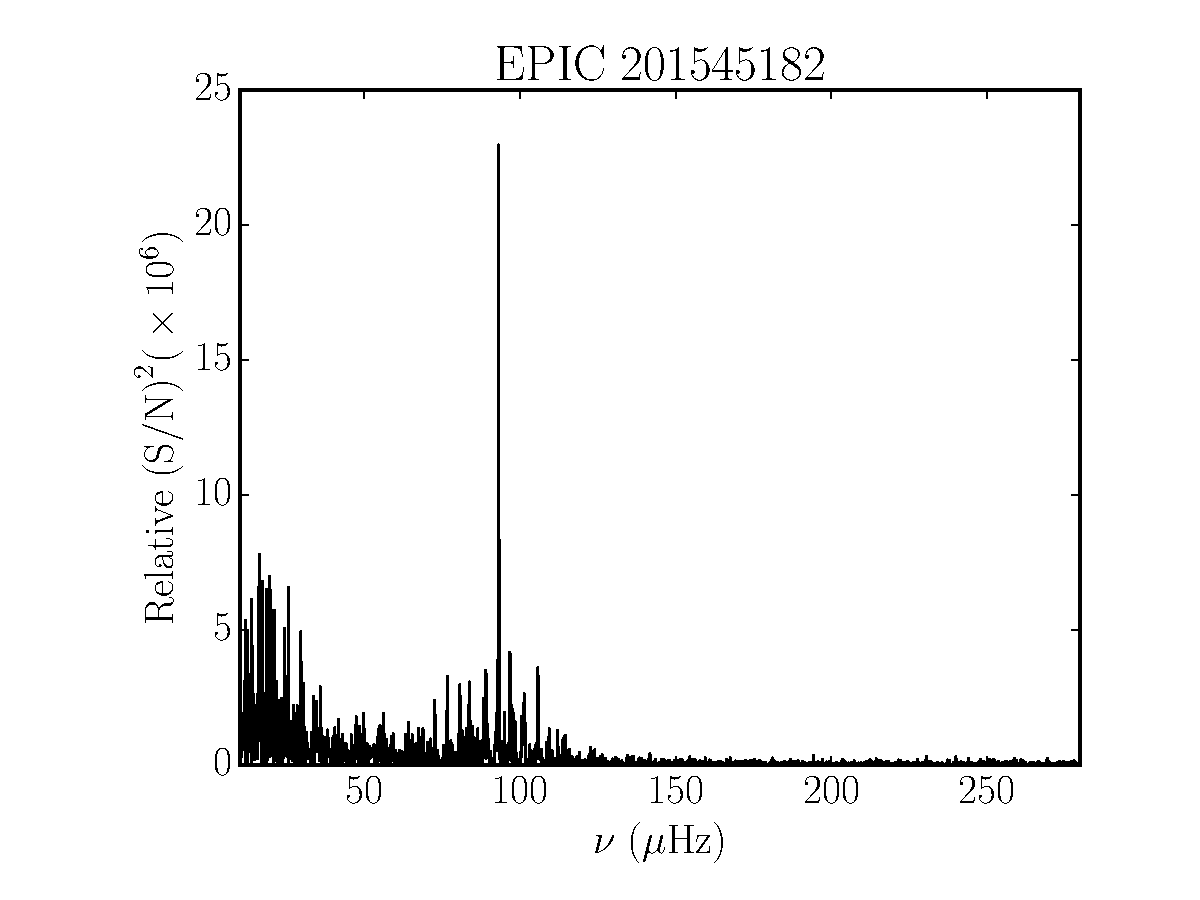
\includegraphics[width=3in]{figures/201545182.pdf}
        }
	\subfigure[]{
            \label{fig:3}
	    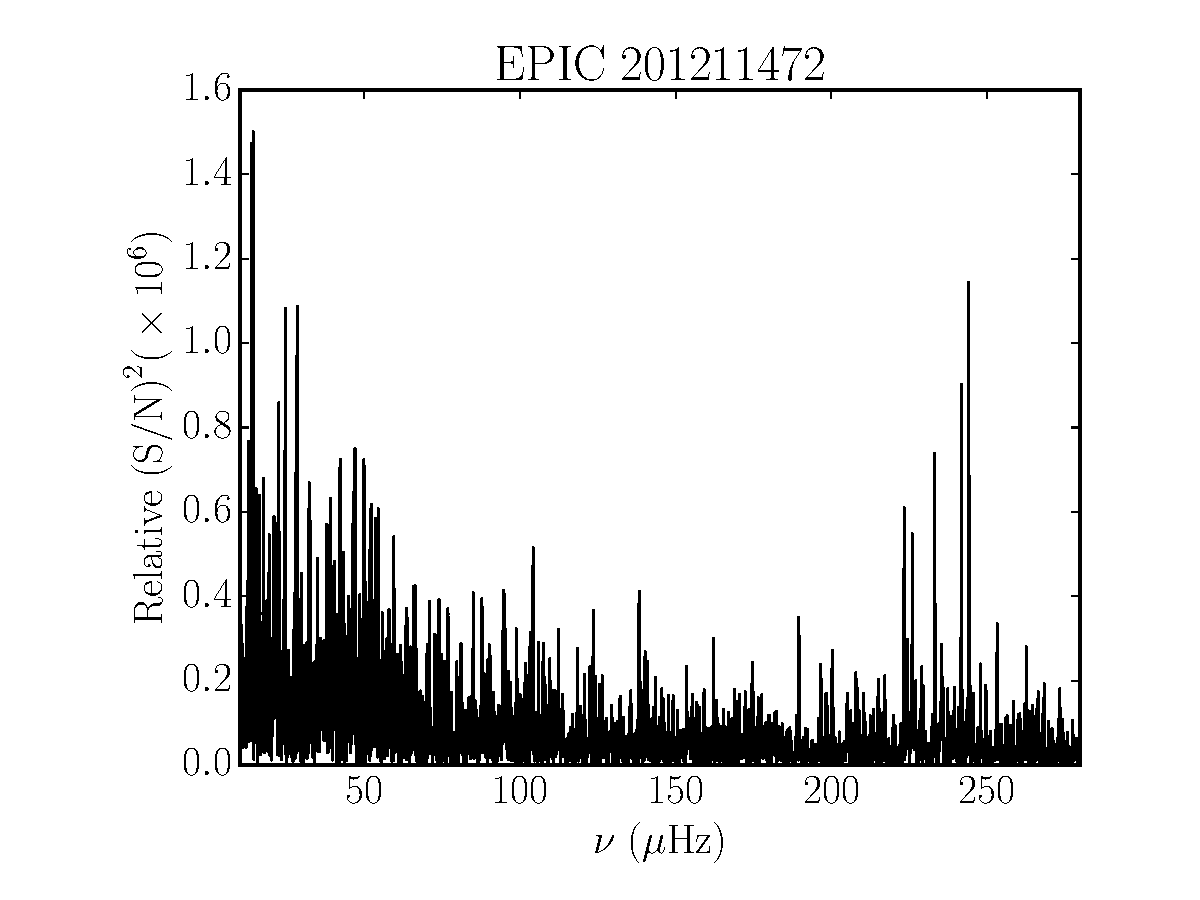
\includegraphics[width=3in]{figures/201211472.pdf}
        }
	\subfigure[]{
            \label{fig:4}
	    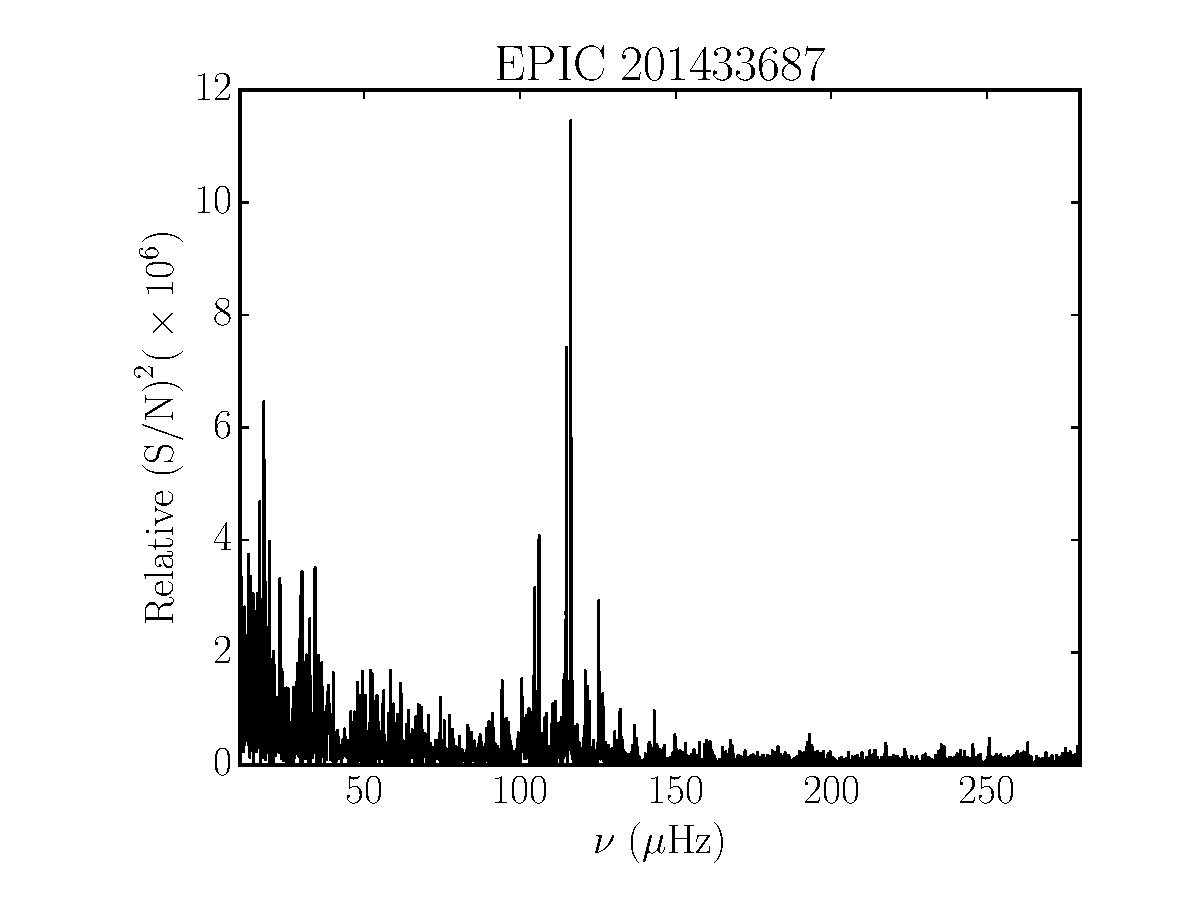
\includegraphics[width=3in]{figures/201433687.pdf}
        }
	\subfigure[]{
            \label{fig:5}
	    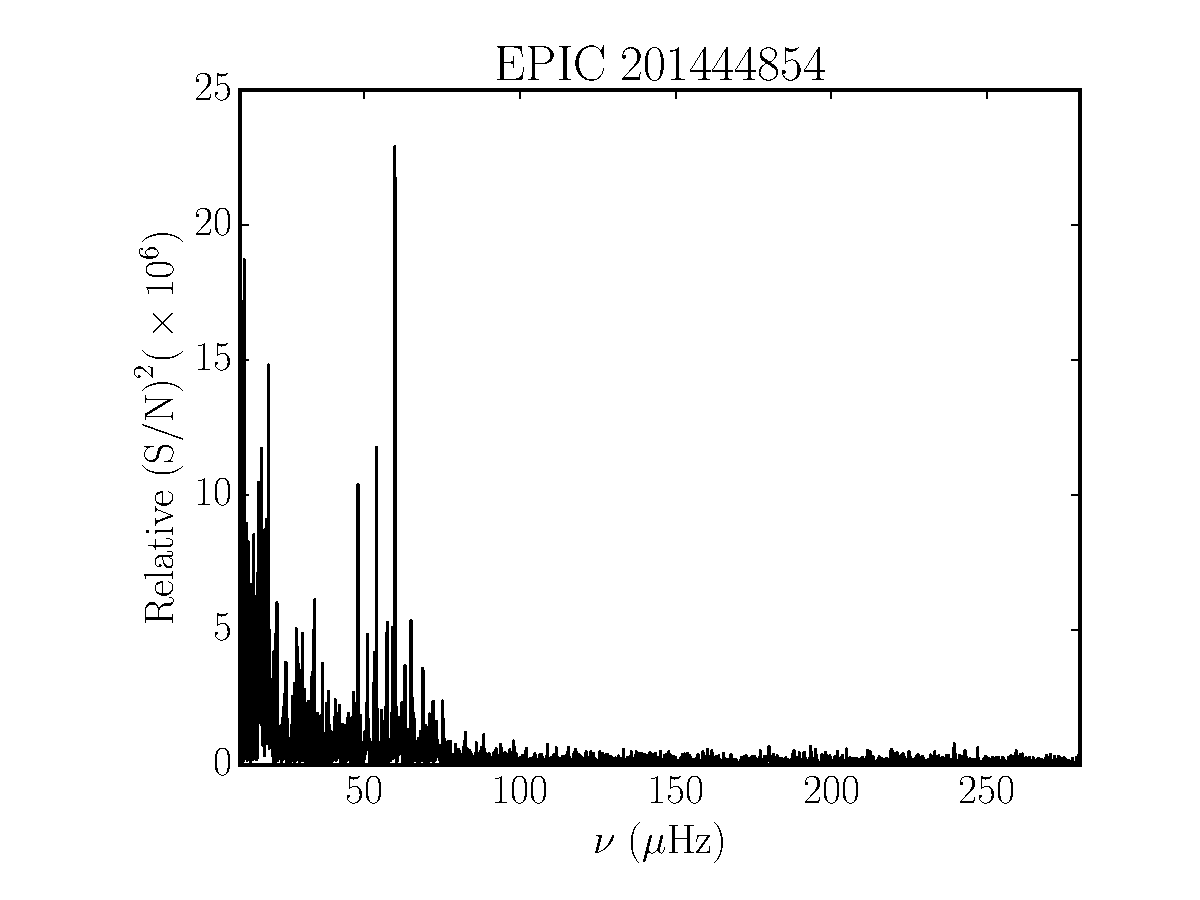
\includegraphics[width=3in]{figures/201444854.pdf}
        }
	\subfigure[]{
            \label{fig:6}
	    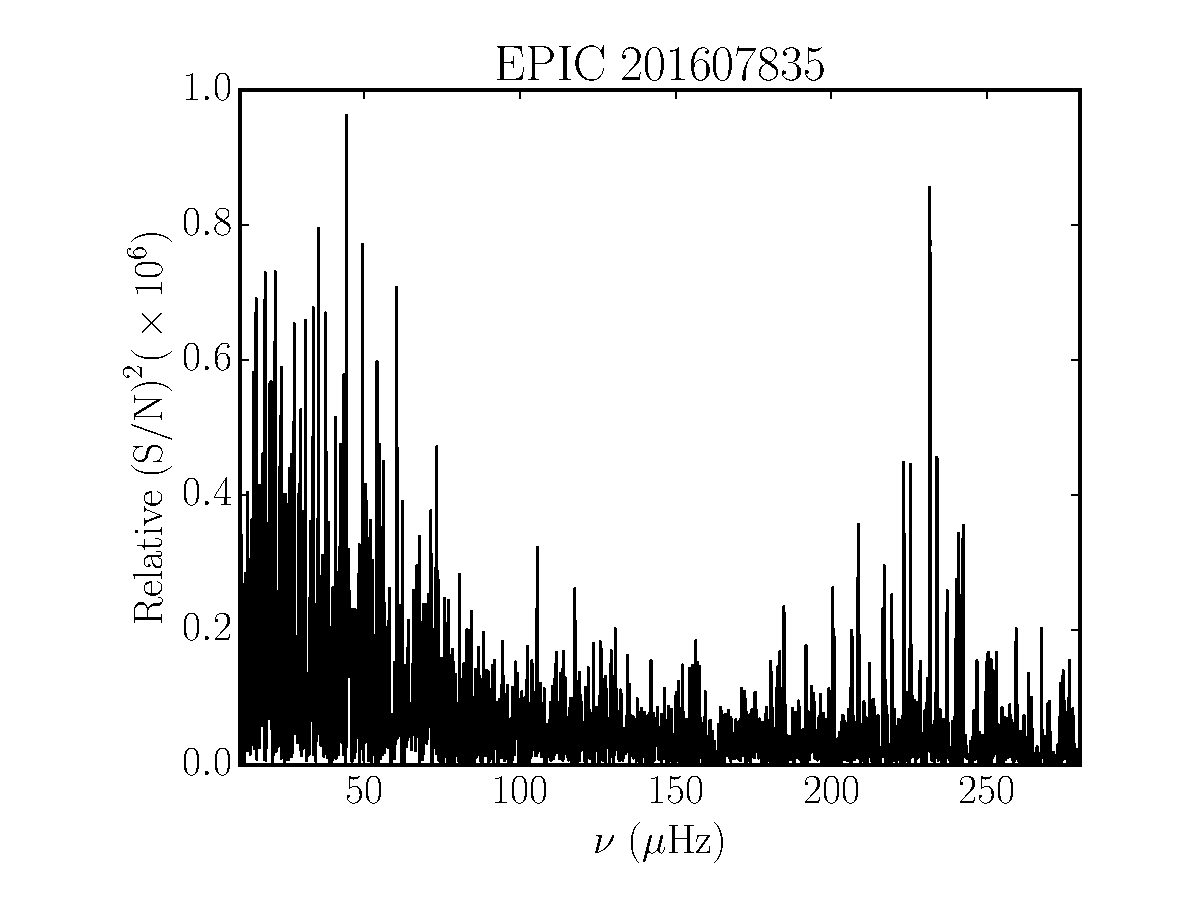
\includegraphics[width=3in]{figures/201607835.pdf}
        }
    \end{center}
    \caption[SIPs of oscillating red giants.]
{SIPs of 6 long cadence {\it K2} giants with asteroseismic
	    oscillations.
	    These were selected from the guest observing program, GO1059 and
	    identified using the method of \citet{Huber2009}.
\label{fig:astero_examples}}
\end{figure}

The top panel of figure \ref{fig:rotation_poster_child} shows the
VJ14-detrended light curve of an active, rotating star, EPIC \rpc, with
a linear trend subtracted off.
The brightness fluctuations clearly visible in the light curve of this target
are produced by cool active regions on the stellar surface, which reduce
the stellar flux periodically.
The rotation period of this star is therefore around 20 days.
The middle and bottom panels show an ACF and LS periodogram of the
detrended light curve.
The top panel of figure \ref{fig:K2_rotation_poster_child} shows the raw light
curve of the same target in grey,  with the conditioned light curve in black.
This conditioned light curve was produced by removing the best fitting
systematic trends, described by a certain combination of the ELCs, at the best
fitting period of the sinusoid.
The bottom panel shows the SIP.

\begin{figure*}
\begin{center}
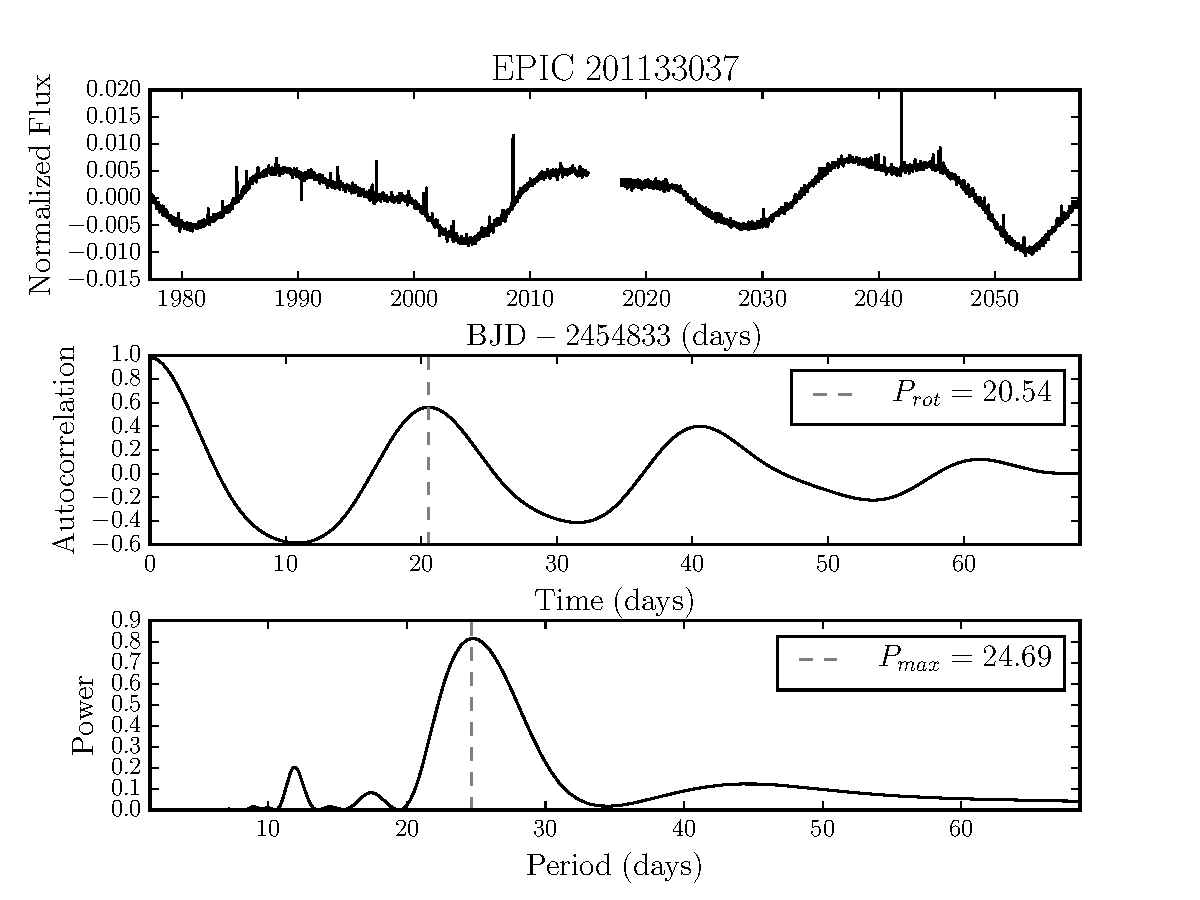
\includegraphics[width=6in, clip=true]{figures/rotation201133037.pdf}
\caption[Example 1: an ACF and LS periodogram of a detrended light curve.]
{{\it Top}: Light curve of EPIC 201133037, detrended using the method
	of VJ14.
	{\it Middle}: Autocorrelation function of the detrended light
	curve. The autocorrelation function method measures a rotation period
	of 21 days for this star.
	{\it Bottom}: The LS periodogram of the detrended light curve.
	The highest peak in the periodogram is located at 25 days.}
\label{fig:rotation_poster_child}
\end{center}
\end{figure*}

\begin{figure*}
\begin{center}
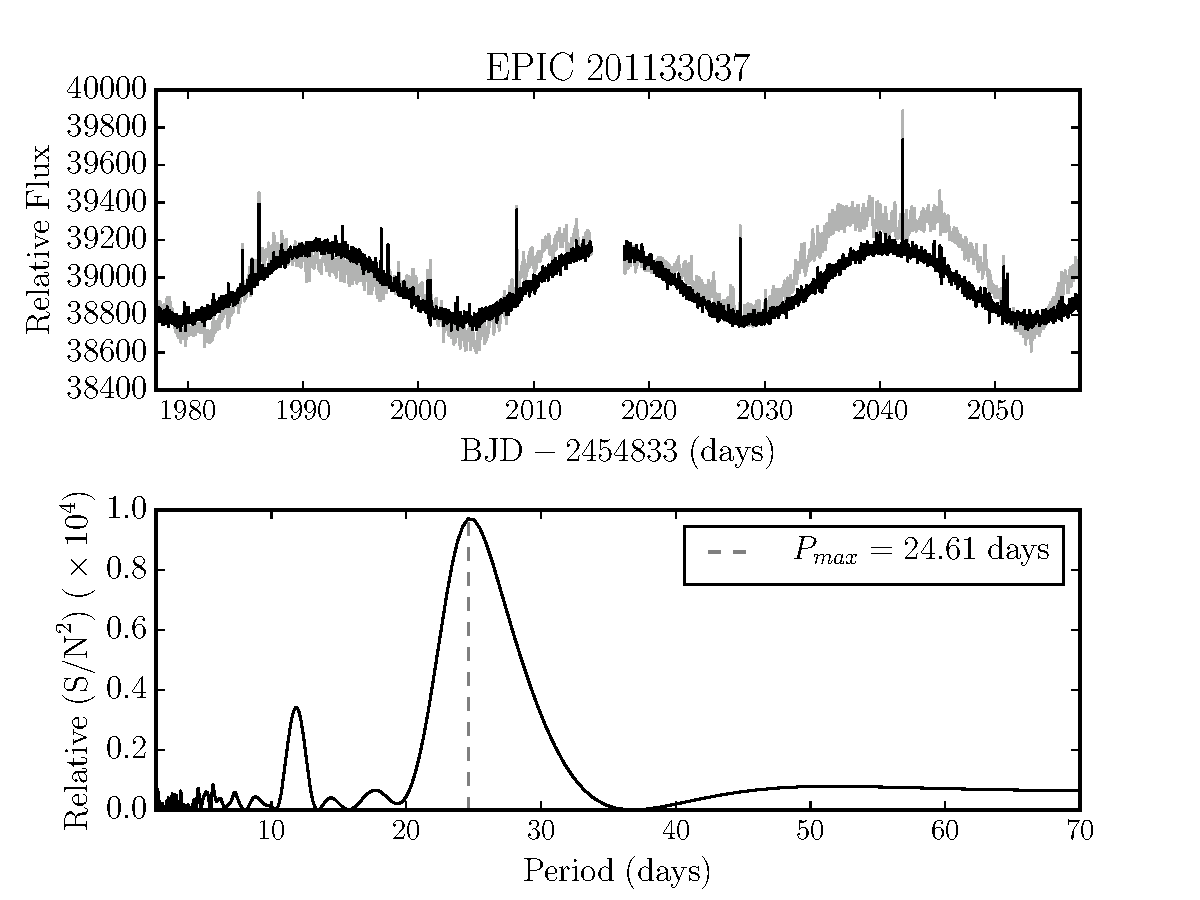
\includegraphics[width=6in, clip=true]{figures/K2_rotation_201133037.pdf}
\caption[Example 1: A SIP with a conditioned light curve.]
{{\it Top}: The raw light curve of EPIC \rpc\ is shown in grey and
	the conditioned light curve is shown in black. The conditioned light
	curve is produced by removing the trends that best describe the
	data, at the best fitting frequency. {\it Bottom}: An SIP of the raw
	light curve, produced by modelling the data using the top 150 ELCs
	plus a sine and cosine function at a range of frequencies.
	The highest peak in the SIP is located at 25 days.}
\label{fig:K2_rotation_poster_child}
\end{center}
\end{figure*}

Each of these three methods measures a rotation period of around 20 days for
this target.
This example demonstates the ability of the SIP to recover rotation periods
that agree with those measured from detrended light curves by autocorrelation.
We also include an example that demonstrates the ability of the SIP to
outperform a periodogram of detrended data.
Figure \ref{fig:rotation_poster_child2} shows the light curve, ACF and LS
periodogram of another rotating star, EPIC \rpcc\ and figure
\ref{fig:K2_rotation_poster_child2} shows its SIP.
This star shows lower amplitude variability than the previous example and the
careful treatment of systematics is much more important.
Whereas the ACF method is able to measure a rotation of $\sim$ 3 days for
this star, the LS periodogram of the detrended light curve incorrectly
measures a period of 59 days.
Although there is a small peak at the rotation period of the star, it is not
the dominant periodic signal.
The SIP method is, by definition, insensitive to these long-term systematics
and is able to measure a period of $\sim$ 2 days.
This example further demonstrates the fact that long-term systematic trends
caused by slow pointing variations are often not removed by conventional
detrending methods.
The 59 day signal is almost certainly a systematic trend and not an
astrophysical signal because it does not appear in the SIP.
It is well described by the ELCs and must therefore be common to many stars.
Although these examples demonstrate that the SIP can provide rotation periods,
in practise it is likely to suffer from overfitting.
Several ELCs contain smoothly varying signals on time scales of a few days to
tens of days which look similar to signals produced by stellar rotation.
In some cases it may be possible to reproduce stellar rotation signals in a
\ktwo\ light curve using only the ELCs, with no additional sinusoid.
We are still investigating the nature of this potential over-fitting problem,
but a solution may to regularise the SIP --- apply priors to the weights of
the ELCs.

\begin{figure*}
\begin{center}
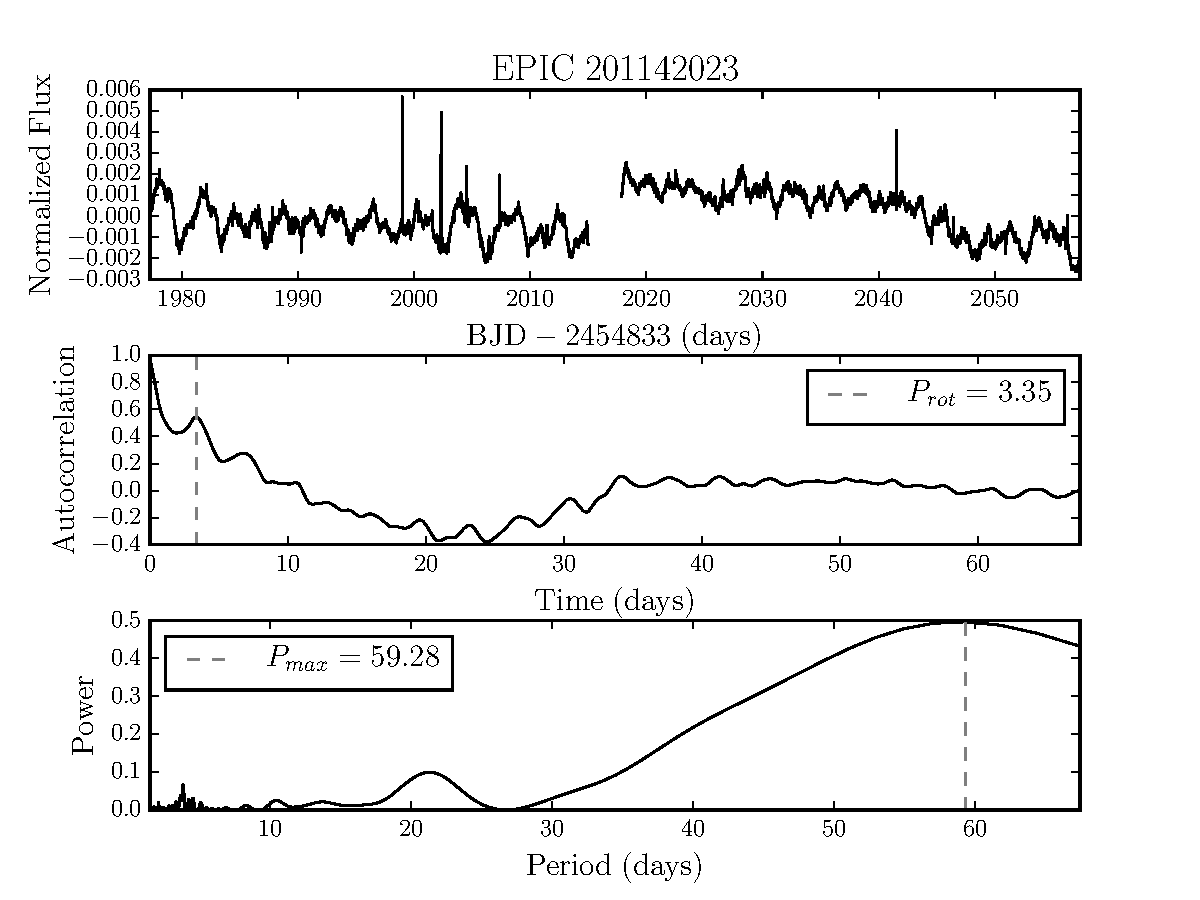
\includegraphics[width=6in, clip=true]{figures/rotation201142023.pdf}
\caption[Example 2: an ACF and LS periodogram of a detrended light curve.]
{{\it Top}: Light curve of EPIC \rpcc, detrended using the method
	of VJ14.
	{\it Middle}: Autocorrelation function of the detrended light curve.
	The autocorrelation function method measures a rotation period of 3
	days for this star.
	{\it Bottom}: The LS periodogram of the detrended light curve.
	The highest peak in the periodogram is located at 59 days and is likely
	to be a systematic trend produced by spacecraft pointing variations.}
\label{fig:rotation_poster_child2}
\end{center}
\end{figure*}

\begin{figure*}
\begin{center}
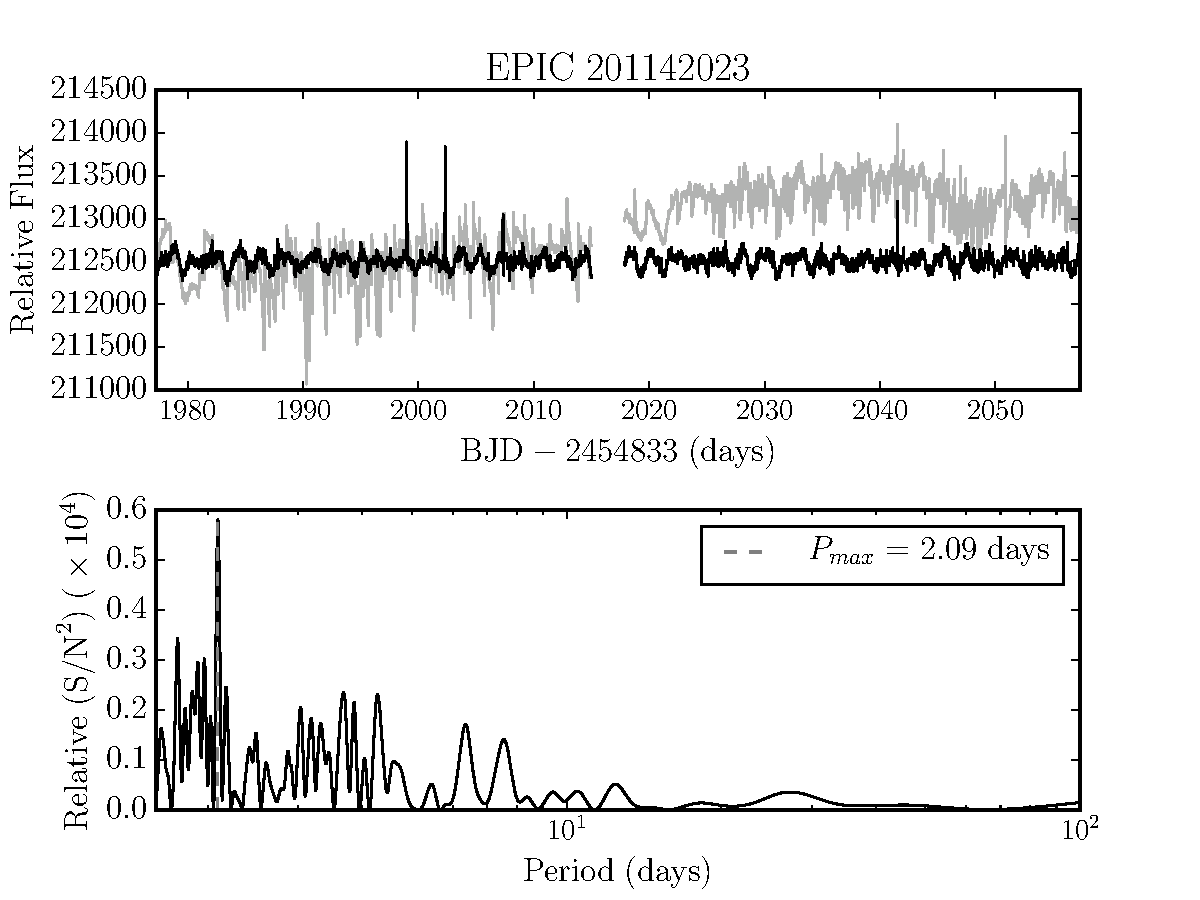
\includegraphics[width=6in, clip=true]{figures/K2_rotation_201142023.pdf}
\caption[Example 2: A SIP with a conditioned light curve.]
{{\it Top}: The raw light curve of EPIC \rpcc\ is shown in grey and
	the conditioned light curve is shown in black. The conditioned light
	curve is produced by removing the trends that best describe the
	data, at the best fitting frequency.
	{\it Bottom}: An SIP, produced by modelling the data as a linear
	combination of the top 150 ELCs plus a sine and cosine function at a
	range of frequencies, measuring a rotation period of 2 days.
	The SIP is, by definition, insensitive to the long-timescale
	systematics that dominate the LS periodogram of the detrended data,
	shown in figure \ref{fig:rotation_poster_child2}.}
\label{fig:K2_rotation_poster_child2}
\end{center}
\end{figure*}

We have shown that the SIP method is able to measure stellar rotation periods
and does better than producing periodograms from detrended data.
However, it has been shown that the ACF method often performs better than
periodogram methods in general for measuring stellar rotation periods
\citep[][]{Mcquillan2013, Mcquillan2014, Mazeh2015}.
For stars with relatively high-amplitude variability, for which perfect
removal of systematic trends is less important, performing the ACF method
on detrended data is likely to produce similar results to the SIP method.
The SIP method is ideally suited to low-amplitude cases, where systematic
trends could drastically influence rotation period measurements.
Whilst the SIP method may outperform ACF in the low-amplitude cases,
any `marginal' rotation period measurements calculated using either method
should be treated with caution unless a representative uncertainty is provided.
In general neither ACF nor periodogram methods are equipped to provide
such uncertainties.
In practise, we recommend using both the SIP and ACF methods, in combination
with a by-eye check, to measure rotation periods for {\it K2} stars.

\subsection{Tests and discussion}

In order to demonstrate the consistent ability of the SIP method
to remove the signal at 47\uHz, corresponding to the periodic $\sim$6 hour
thruster firings, we computed SIPs for \nGO\ targets from the GO1049
proposal: ``Galactic Archaeology on a grand scale" (PI: Stello, D.).
For each target, an SIP of its raw photometry and a LS periodogram of its
VJ14 light curve was calculated for frequencies between
40 and 54 \uHz.
Both the height and frequency of the highest peak in the SIP and the highest
peak in the LS periodogram were recorded.
A histogram of the frequencies of the highest peaks in the SIPs of all \nGO\
targets is shown in the top panel of figure \ref{fig:sip_hist}.
The bottom panel shows the histograms of peak heights within the
correspondingly colored ranges indicated in the top panel.
This figure shows that while there are a greater number of maximum peaks
around 47 \uHz, the S/Ns of these peaks are comparable to those found just
above and just below this frequency.
Figure \ref{fig:vbg_hist} shows the equivalent results for the
VJ14 light curves.
There is a significant number of large peaks at $\sim$47 \uHz\ in the LS
periodograms of the detrended light curves; the highest peak in the LS
periodograms was almost always located at $\sim$ 47 \uHz.
Furthermore, the distribution of peak power within the range 46.5-48 \uHz\ is
skewed towards higher powers, i.e. a substantial fraction of the peaks at
$\sim$ 47 \uHz\ have a large power.
The SIP method is able to consistently remove the 47 \uHz\ signal which is
present in almost every VJ14 light curve.

We performed an injection and recovery experiment in order to test the
detection efficiency of the SIP algorithm.
\Ninjections\ sinusoids with frequencies ranging from 10-270 \uHz\ and
amplitudes ranging from \minamp\ to \maxamp\ parts-per-million were injected
into the raw \ktwo\ light curve of target star EPIC 201121245, a relatively
non-variable giant with low-amplitude acoustic oscillations.
In order to recover the injected signals we calculated a SIP of the original
light curve, subtracted this from the SIP of injected light curve,
and searched for excess power in the residuals.
This allowed us to perform injection and recovery tests on this target star
without being affected by the star's own intrinsic variability.
We then measured the position of the highest peak in the resulting residual
SIP and recorded the successful detections, defined as those that lay within
1 \uHz\ of the injected value.
SIPs were computed over a grid of frequencies ranging from 10-270 \uHz, with
a spacing of 0.1 \uHz.
The resulting detection efficiency map is shown in figure \ref{fig:map}.
This figure demonstrates that the SIP can recover the frequencies of signals
with amplitudes less than 10 ppm.
% The frequency precision of the recovered signals is set by the length of the
% \ktwo\ campaigns; an observing window of 90 days

\begin{figure*}[h]
\begin{center}
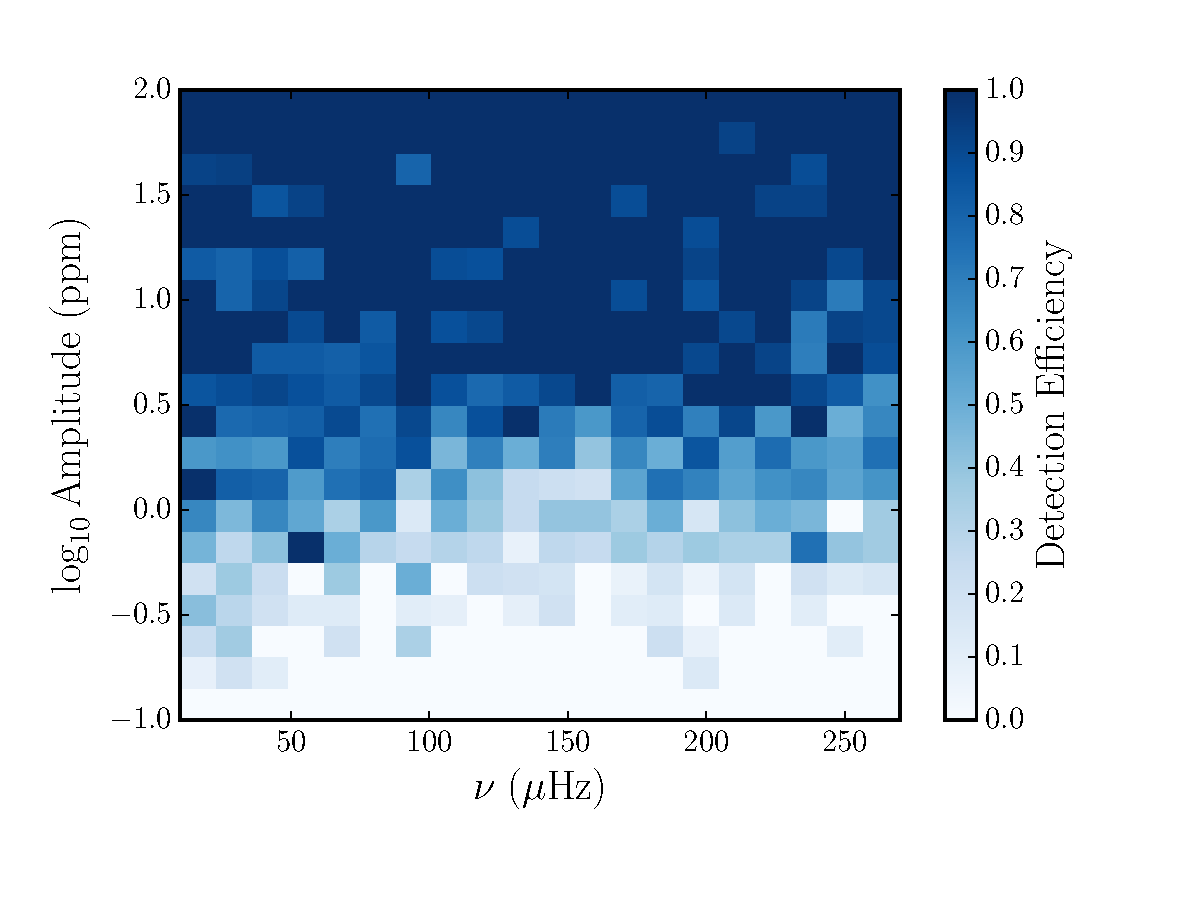
\includegraphics[width=6in, clip=true]{figures/hist.pdf}
\caption[SIP detection efficiency.]
{A map of the detection efficiency of the SIP algorithm as a function
of frequency and injection amplitude. The SIP is capable of recovering
signals with amplitudes less than 10 ppm.}
\label{fig:map}
\end{center}
\end{figure*}

\begin{figure*}[h]
\begin{center}
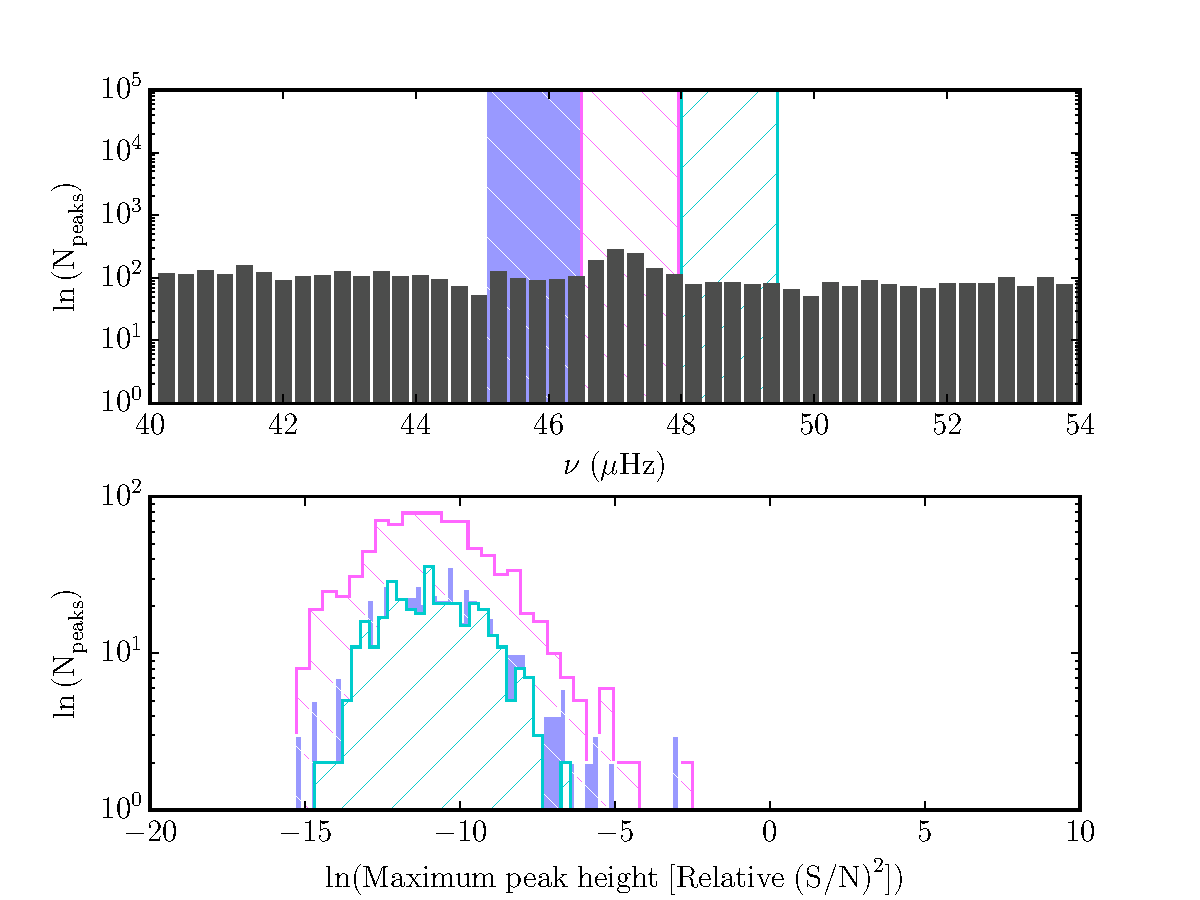
\includegraphics[width=6in, clip=true]{figures/sip_hist.pdf}
\caption[How insensitive is the SIP?]
{{\it Top:} Histogram of the frequencies of the highest peaks in the
	SIPs of \nGO\ {\it K2} targets within the range 40--54 \uHz.
	{\it Bottom:} Histograms of peak heights within the correspondingly
	colored ranges indicated in the top panel.
	Whilst there is a larger number maximum peaks around 47 \uHz\ (the
	frequency corresponding to the 6 hour thruster fire) the amplitudes of
	these maximum peaks are comparable to the maximum peak heights just
	above and just below this frequency.}
\label{fig:sip_hist}
\end{center}
\end{figure*}

\begin{figure*}[h]
\begin{center}
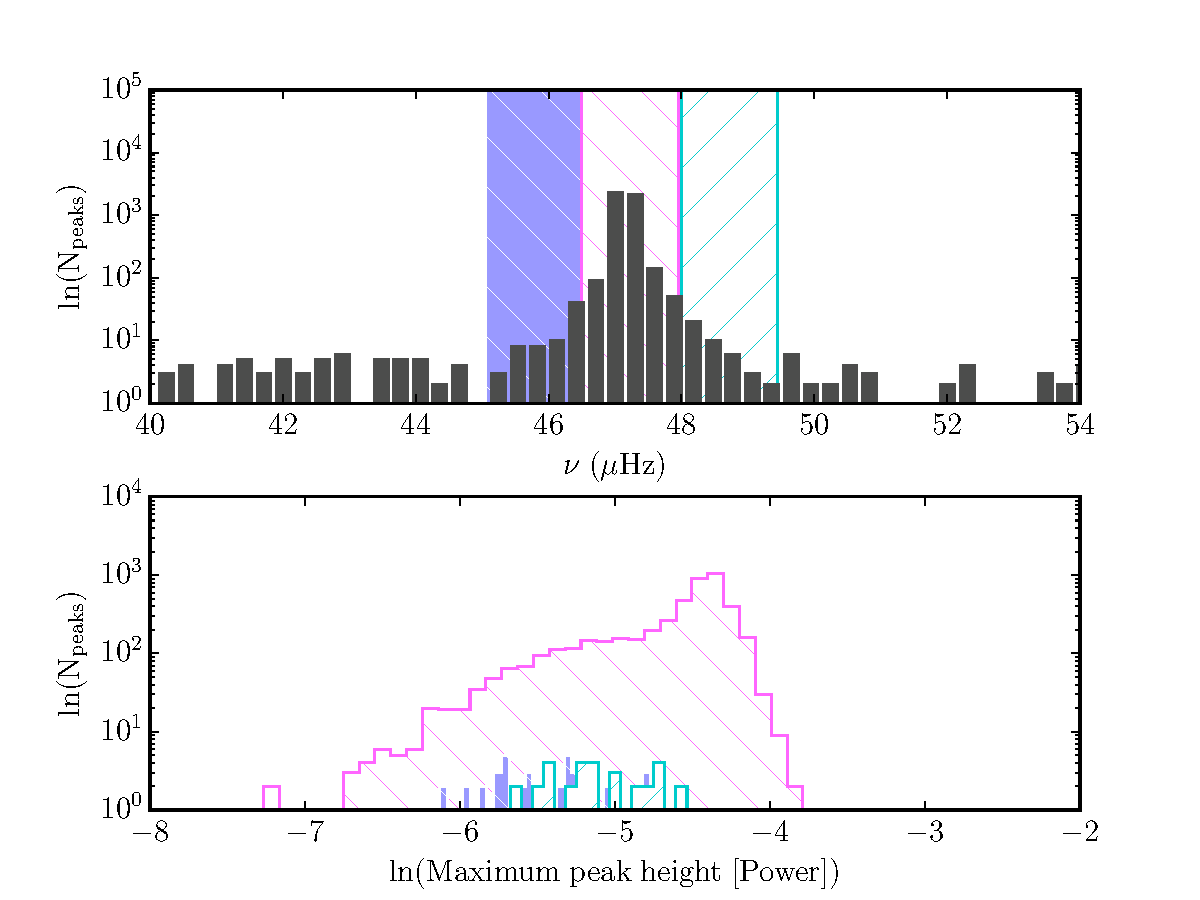
\includegraphics[width=6in, clip=true]{figures/vbg_hist.pdf}
\caption[Thruster firing signals in \ktwo\ light curves.]
{{\it Top:} Histogram of the frequencies of the highest peaks in the
	LS periodograms of the \citet{Vanderburg2014} light curves of \nGO\
	{\it K2} targets within the range 40--54 \uHz.
	{\it Bottom:} Histograms of peak heights within the correspondingly
	colored ranges indicated in the top panel.
	The frequency of maximum peak height was $\sim$ 47 \uHz\ in almost
	every periodogram.
	Furthermore, the distribution of maximum peak height within the range
	46.5-48 \uHz\ is skewed towards higher powers, i.e. a large fraction of
	the peaks at $\sim$ 47 \uHz\ have a large power.
}
\label{fig:vbg_hist}
\end{center}
\end{figure*}

Figure \ref{fig:planet} shows the conditioned light curve and SIP of the
short-period, disintegrating planet candidate discovered by
\citet{Sanchis-Ojeda2015}.
This planet has a period of around 9 hours, short enough to be detectable
with a periodogram, as was demonstrated for a number of ultra-short
period {\it Kepler} exoplanets by \citet{Sanchis-Ojeda2014}.
The top panel of this figure shows the {\it K2} light curves of these
objects, conditioned on the highest S/N sinusoidal signal in the
periodograms.
The light curve was produced by subtracting the trends that best describe
the data at the highest S/N period found in the SIP.

\begin{figure*}
\begin{center}
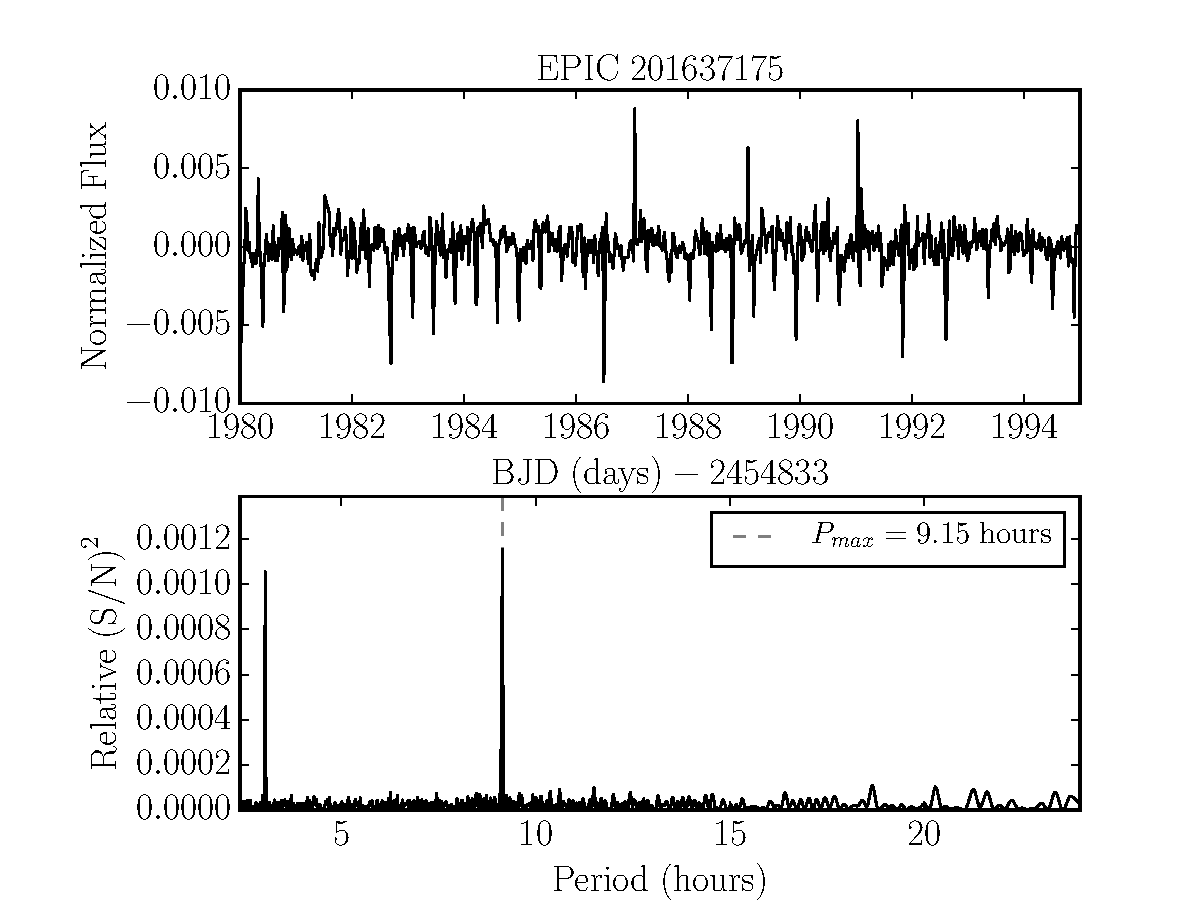
\includegraphics[width=6in, clip=true]{figures/planet_201637175.pdf}
\caption[Exoplanets with the SIP]
{{\it Top:} The light curve of exoplanet candidate, EPIC 201637175,
	conditioned on the highest amplitude sinusoidal signal found in the
	periodogram. {\it Bottom:} The systematic-insensitive periodogram of
	this target.}
\label{fig:planet}
\end{center}
\end{figure*}

Photometric variability in dwarf stars on timescales less than 8 hours, often
known as flicker, has been linked to surface gravity
\citep[][]{Bastien2013, Kipping2014}.
The metrics used to quantify photometric variability include finding the range
in intensity, counting the number of zero crossings and calculating the
root-mean-square (RMS) of the light curve.
Although these features are related to signal processing, they are operations
performed on detrended light curves, not inferred from periodograms.
However, it may be possible to derive a property of the periodogram that scales
with the density or surface gravity of a star, for example, the mean excess
power at frequencies near those relevent to granulation timescales.
The SIP method presented here would be useful for such a technique.

\section{Conclusions}
\label{sec:conclusions}
We demonstrate that modelling campaign 1 {\it K2} photometry as a linear
combination of 150 PCA components plus a sinusoid can produce periodograms
that are almost completely free from instrumental systematic signals, without
the need for detrending.
We find that the 47 $\mu$Hz signal, generated by the spacecraft thruster
fires is not present in the vast majority of Systematics-Insensitive
Periodograms (SIPs) for more than 4000 targets
selected from the {\it K2} guest observer program, GO1059, ``Galactic
Archaeology on a grand scale" (PI: Stello, D.).
The SIP method is highly successful for campaign 1 targets where the large
number of stars, observed for a baseline of 80 days ensures that most of the
systematics are captured in the ELCs and we anticipate that it will
be equally effective for the up-and-coming campaigns.

The SIP method is capable of detecting periodicities in {\it K2} data in the
region of frequency space relevent to the study of asteroseismic oscillations
in giant stars and for any signals with a timescale close to 6 hours.
It may be useful for measuring stellar rotation periods and is an improvement
upon a simple LS periodogram of detrended data, however rotation period
inference with the SIP may suffer from over-fitting.
We intend to address this problem in future by developing a regularised
version of the SIP.
In practise, the best approach for measuring rotation periods in {\it K2} data
is likely to be a combination of the SIP method and the ACF method, where
autocorrelation is performed on detrended light curves.

Of course, as mentioned in chapter \ref{chapter:intro}, a sinusoid is actually
{\it not} a good model for stellar rotation signals.
For this reason, the SIP's usefulness for measuring rotation periods is
limited.
In the following chapter I introduce an alternative method for inferring
rotation periods, using a semi-parametric function (a Gaussian process).
It will be possible to combine this Gaussian process model with the same noise
model used by the SIP to produce a GPSIP (Gaussian Process
Systematics-Insensitive Periodogram).
Indeed, any model could be used in place of a sinusoid, although linear models
have an advantage in computational efficiency and a GPSIP would be extremely
expensive.
Still, it would be worth exploring the performance of the GPSIP in the future.

The SIP code is available for public use and can be found at
\url{https://github.com/RuthAngus/SIPK2}.

\chapter{Stellar rotation period inference using Gaussian processes}
\label{chapter:GP}

\begin{abstract}
The light curves of spotted, rotating stars are often non-sinusoidal and
quasi-periodic---spots are not static on the stellar surface and have finite
lifetimes causing stellar flux variations to slowly shift in phase.
A strictly periodic sinusoid is therefore not a representative generative
model for the light curve of star with a rotational signal.
Ideally, a physical model of the stellar surface would be conditioned on the
data, however the parameters of such models can be highly degenerate
\citep[\eg][]{Russell1906, Jeffers2009}.
Instead, we use an appropriate {\it effective} model: a Gaussian Process (GP)
with a quasi-periodic covariance kernel function.
By modelling the covariance matrix of the light curve with a GP, a highly
flexible semi-parametric function, we avoid the necessity to choose a `best
fitting' functional form, whilst sampling directly from the posterior
probability distribution function of the periodic parameter and marginalising
over the other kernel hyperparameters.
We used \nlightcurves\ simulated light curves with a range of rotation periods
to test the GP model.
We attempted to recover the rotation periods using three methods: our GP
method, a sine-fitting periodogram method and an autocorrelation function
method.
The posterior probability distribution of the rotation period parameter was
sampled using the affine invariant ensemble MCMC sampler {\tt emcee}
\citep{Foreman-Mackey2013}, and the GP operations were performed using the
{\tt george} python package \citep{George}.
Rotation periods inferred via this method are more precise and accurate than
the periodogram and ACF methods.
Furthermore, the improvement is expected to be even more dramatic when applied
to real, noisy {\it Kepler} light curves, since the GP method is well suited
to modelling rotation signals and correlated noise simultaneously.

\end{abstract}

\section{Introduction}

The light curves of spotted, rotating stars are often non-sinusoidal and
Quasi-Periodic (QP).
These stars vary in brightness due to active regions on their surfaces which
rotate in and out of view.
The non-sinusoidal quality is caused by the complicated surface spot patterns
and the quasi-periodicity is produced both by the finite lifetimes of these
active regions and the presence of differential rotation on the stellar
surface.
A strictly periodic sinusoid is therefore not a good model for stellar light
curves.
In an ideal world, a physical model of the stellar surface would be
conditioned on the data.
A physically realistic, generative model would perfectly capture the complexity
of shapes within stellar light curves as well as the quasi-periodic nature,
allowing for extremely precise probabilistic period recovery.
However, such physical models require many free parameters in order to
accurately represent a stellar surface and some of these parameters are
extremely degenerate \citep[\eg][]{Russell1906, Jeffers2009}.
In addition to global stellar parameters such as inclination and rotation
period, each spot or active region should have (at minimum) a longitude,
latitude, size, temperature and lifetime.
Considering that many stars have on the order of hundreds of spots, the number
of free parameters quickly becomes unwieldy, especially if the posterior PDFs
of these parameters are explored with MCMC.
Simplified spot models, such as the one described in \citet{Lanza2014} where
only two spots are modelled, have produced successful results, however these
simplified models sacrifice some precision due to lack of model flexibility.
Instead of using a physical model for stellar light curves, we choose to use
an {\it effective} model: one which captures the behaviour but is not
physically motivated, although the parameters of this model may be {\it
interpreted} as physical ones.
An ideal effective model for the light curve of a spotted, rotating star is
one with a small number of non-degenerate parameters that is flexible enough
to perfectly capture non-sinusoidal, QP behaviour.
These requirements are perfectly fulfilled by a Gaussian process (GP) model.

The standard methods used for measuring rotation periods include detecting
peaks in a Lomb-Scargle \citep{Lomb1976, Scargle1982} (LS) periodogram
\citep[e.g.][]{Reinhold2013}, Auto-Correlation Functions (ACFs)
\citep{Mcquillan2013} and wavelet transforms \citep{Garcia2014}.
The precision of the LS periodogram and wavelet methods are limited by the
suitability of the model choice.
A sinusoid is used in the case of the LS periodogram and the wavelet method
relies on a choice of mother wavelet that is assumed to describe the data over
a range of transpositions \citep[see, \eg][]{Carter2010}.
In contrast, the ACF method is much better suited to signals that are
non-sinusoidal.
In fact, it doesn't matter what shape the signal is: as long as it is
approximately periodic the ACF will display peaks located at the rotation
period.
A drawback of the ACF method however, is that it requires data to be
evenly-spaced\footnote{\citet{Edelson1988} describe a method for computing
ACFs for unevenly-spaced data.} which is not the case with \Kepler\ light
curves (although in many cases it can be approximated as uniformly sampled).
An ACF is also an operation performed on the data, not a generative model of
the data and is therefore not inherently probabilistic.
For this reason it is very difficult to estimate the uncertainty on an ACF
rotation period measurement.
Many rotation periods in the literature have been inferred by measuring the
position of the first peak in an ACF, however this approach can be dangerous.
The exponential decay in correlation can shift the peak position short-wards
of its true value, leading to an underestimate of the period.
We return to this point in section \textsection \ref{sec:discussion}.
% In order to avoid this, a period should be inferred by modelling the entire
% ACF, not just measuring the position of the first peak.

The motivation for developing a GP-based method for rotation period inference
is, firstly to measure more accurate and precise rotation periods using a
better-suited generative model than a sinusoid for the reasons explained
above.
Secondly, in order to infer {\it probabilistic} periods, i.e. to estimate the
posterior PDF of the rotation period and thereby measure a realistic and
representative uncertainty.
And thirdly, to allow for an additional correlated noise model to be included
during regression, the parameters of which could be marginalised over.
% And fourthly to provide some way of determining whether a periodic model is
% supported by the data over a purely stochastic one.

GPs are commonly used in the machine learning community and increasingly
in other scientific fields, for example biology and geophysics (where GP
regression is called `kriging').
More recently, GPs have been used in the astronomy literature \citep[see
\eg][]{Gibson2012, Haywood2014, Haywood2015, Evans2015, Rajpaul2015,
Rajpaul2016, Aigrain2016}.
% FIXME: CITATIONS Gibson, Aigrain, Evans, Rajpaul, Waldman(?), Cosmology,
% geology, biology, Rasmussen & Williams, etc.
They are useful in regression problems involving any stochastic process,
specifically when the probability distribution for the process is a
multi-variate Gaussian.
If the probability of obtaining a data-set is a Gaussian in $N$ dimensions,
where $N$ is the number of data points, that data-set can be described as, and
with, a Gaussian process.
An in-depth introduction to Gaussian processes is provided by
\citet{Rasmussen2005}.

GP models parameterise the covariance between data points and a kernel
function provides the form of covariance matrix parameterisation.
For example, take the time-series in figure \ref{fig:GP_example}.
% This is a \kepler\ light curve of Earth-like planet host Kepler-452: a G-type
% star that rotates once every $\sim$ 15 days.
This is the \kepler\ light curve of KID 1430163, a relatively active star that
rotates once every $\sim$ 4 days.
The stochastic variability in this time-series is typical of \kepler\ FGK
stars.
Clearly, data points in this light curve are correlated.
Points that are close together in time are tightly correlated and those that
are far apart are loosely correlated.
It is the way in which the covariance varies with the separation between data
points that is modelled when using GP regression.
It is not the data but the {\it covariance structure} that is modelled.
This fact is what gives GPs their flexibility---they can model any time
series with a similar covariance structure.
In addition, a very simple function can usually capture the covariance
structure of a light curve, whereas a much more complicated one may be
required to model the time-series itself.
% The light curve of \Kepler-452 has been modelled with a GP in figure
% \ref{fig:GP_example}, shown in orange.
The light curve of this star has been modelled with two different GP kernel
functions in figure \ref{fig:GP_example}, shown in blue and pink.
Both provide adequate fits to the data, however only the periodic kernel
function, `QP' is a useful model because it has a periodic parameter.
I return to this point shortly.

A range of kernel functions could be used to describe stellar variability.
For example, the simplest and most commonly used kernel function, the `Squared
Exponential' (SE) produces an adequate fit to the KID 1430163 light curve.
The SE kernel function is defined as,
\begin{equation}
k_{i,j} = A \exp \left(-\frac{(x_i - x_j)^2}{2l^2} \right).
\end{equation}
\label{eq:SE}
Here $A$ is the amplitude of covariance, $l$ is the length scale of
exponential decay and $x_i-x_j$ is the separation between data points.
The SE kernel function has the advantage of being very simple---it has just
two parameters, a covariance amplitude and length scale: $A$ and $l$.
If $l$ is large two data points far apart in $x$ will be tightly correlated,
and if small they will be loosely correlated.
Another property of the SE kernel function is that it produces functions that
are infinitely differentiable.
It is therefore possible to model a data set and its derivatives
simultaneously.
% \citep[see \eg][]{Rajpaul2015}
The SE kernel function may be an adequate model of the covariance in stellar
light curves, but it is not a {\it useful} one for the problem of rotation
period inference because it does not have a parameter that describes a period.
In order to infer rotation periods it is necessary to use a periodic kernel
function.
For this reason, we use the `Quasi-Periodic' kernel function.
The QP kernel function is defined as
\begin{equation}
k_{i,j} = A \exp \left(-\frac{(x_i - x_j)^2}{2l^2} -
\frac{\sin^2(\frac{2\pi}{P})}{\Gamma^2} \right).
\end{equation}
\label{eq:QP}
It is the product of the SE kernel function, which describes the overall
covariance decay, and an exponentiated, squared, sinusoidal kernel function
that describes the periodic covariance structure.
$P$ can be interpreted as the rotation period of the star and $\Gamma$
controls the number of zero crossings per period.
This kernel function allows two data points that are separated in time by one
rotation period to be tightly correlated, while points separated by half a
period can be weakly correlated.
Both the QP and SE kernel functions were used to produce the blue and pink
models shown in figure ~\ref{fig:GP_example}.

In order to infer a stellar rotation period from a light curve, we fit a GP
model with a QP kernel function to the data.
The likelihood of the model, conditioned on the data could then be maximised
in order to find the maximum likelihood value for $P$.
In this study however, the full posterior PDFs of the parameters are explored
using MCMC.
This latter approach comes at a cost: a GP model is expensive to compute once
as it requires a matrix inversion and determinant evaluation, let alone the
many thousands of times that is necessary to fully explore the posteriors of
the parameters.
However, fully exploring the posterior PDF of $P$, allows for an accurate
estimate of the uncertainty on the rotation period.

% \begin{figure}
% \begin{center}
% 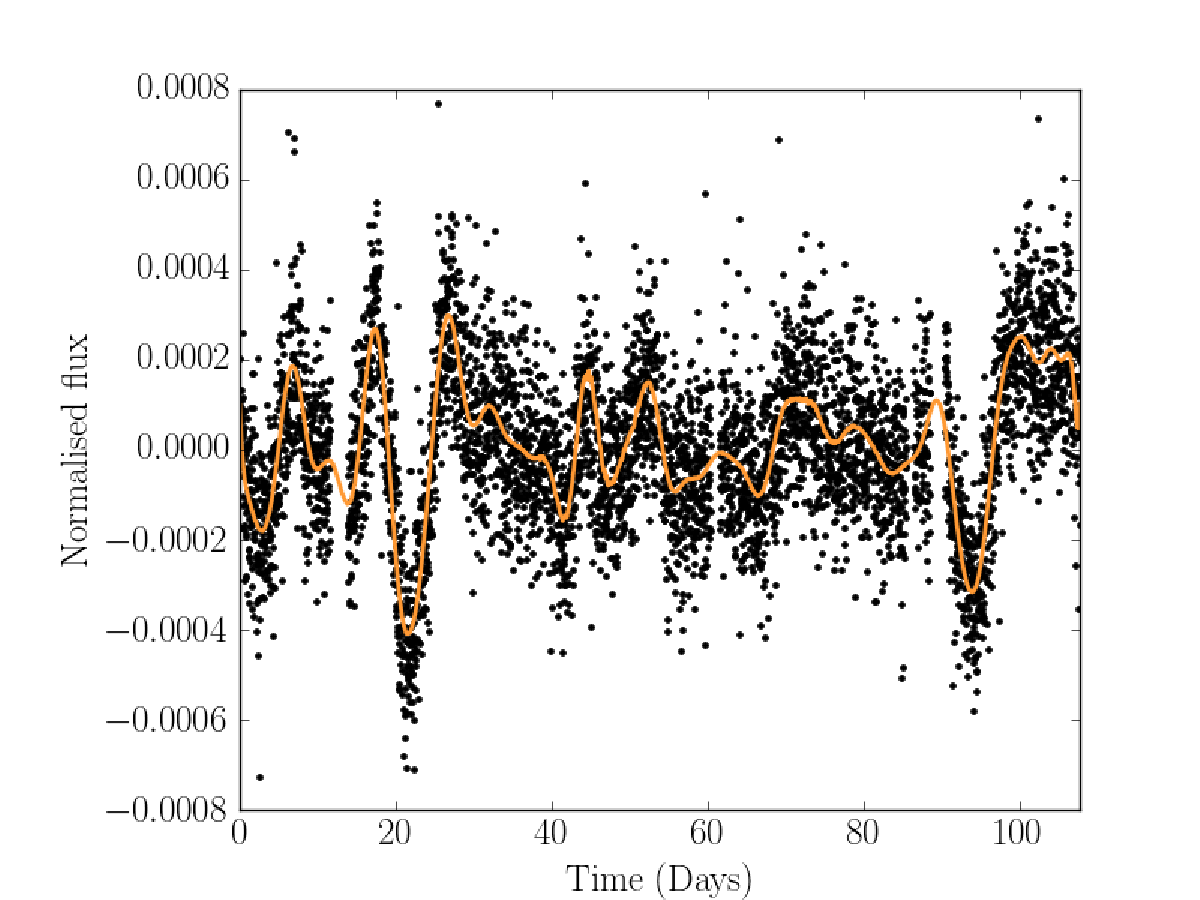
\includegraphics[width=6in, clip=true]{figures/Kepler452b.pdf}
% \caption[A light curve with a GP model.]
% {Light curve of Kepler-452 b, a habitable-zone, Earth-sized planet
% hosting G star \citep{Jenkins2015}. The orange line shows a fit to the data using
% a Gaussian process model with a QP covariance kernel function.}
% \label{fig:GP_example}
% \end{center}
% \end{figure}

\begin{figure}
\begin{center}
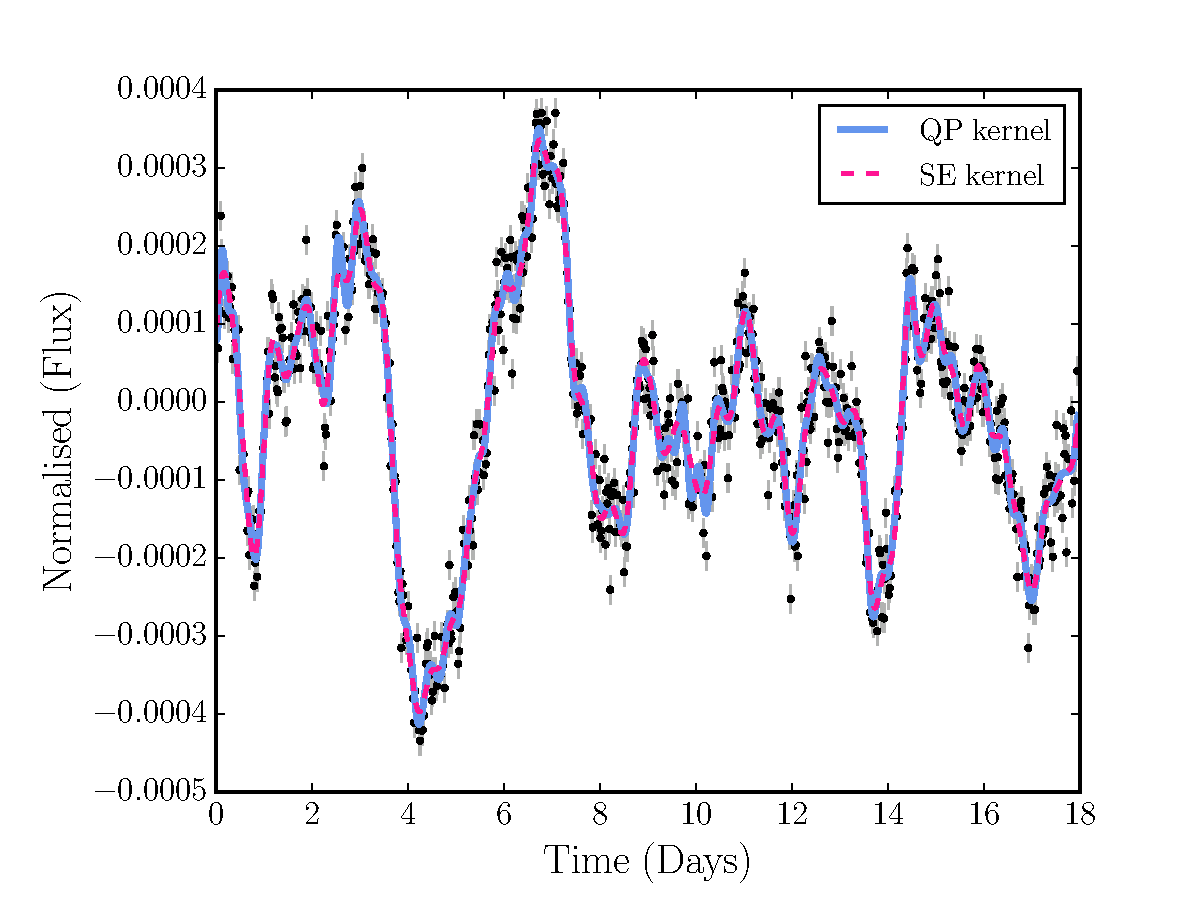
\includegraphics[width=6in, clip=true]{figures/001430163.pdf}
\caption[A light curve with a GP model.]
{Light curve of KID 1430163, an active star with a rotation period of $\sim$ 4
days.
The blue solid line shows a fit to the data using
a Gaussian process model with a QP covariance kernel function and the pink
broken line shows a fit with a SE kernel function.
Both kernel functions provide an adequate fit to the data, however we use the
QP function because it has a useful parameter that corresponds to the star's
rotation period.}
\label{fig:GP_example}
\end{center}
\end{figure}

\section{Rotation period injection and recovery}

In order to test the GP method we attempted to the measure rotation periods of
a set of simulated light curves.
We simulated \nlightcurves\ light curves using a spot model similar to that
used
% We used light curves simulated
for the \citet{Aigrain2015} `hare and hounds' rotation period recovery
experiment.
These light curves were simulated by placing dark, circular spots with slowly
evolving size, on the surface of bright, rotating spheres, ignoring
limb-darkening effects.
\citet{Aigrain2015} simulated one thousand light curves in order to test the
ability of participating teams to recover both the stellar rotation periods
and the rotational shear: the amplitude of surface differential rotation.
% Since we are not interested in recovering differential rotation we only used
% those light curves simulated {\it without} differential rotation, of which
% there are \nlightcurves.
Unlike in their study we are not interested in recovering differential
rotation in this work, so did not include it in our simulations.
We opted to use only solid-body rotators because differential rotation may
produce some additional scatter in the rotation period measurements recovered.
This code can also be adjusted to produce more realistic light curves by
altering spot lifetimes.
Stars with spot lifetimes that are long relative to their rotation periods
will have highly periodic light curves.
Those with short spot lifetimes will be more quasi-periodic.
We fixed the mean spot lifetime at an arbitrary value of 30.5 days for all
light curves in these initial tests.
In future we plan to include both differential rotation and variable spot
lifetimes in our light curve model.
Light curves were simulated with a real \Kepler\ long-cadence time array, with
one data point every thirty minutes over a four year duration.
The rotation periods of the simulations were randomly drawn from a log-uniform
distribution between 0.5-60 days.
Figure \ref{fig:noise-free_lc} shows an example of a simulated, noise-free
light curve with a period of 17.4 days.

% The ranges and distributions of the physical stellar parameters used in the
% simulated light curves are tabulated below, in table
% \ref{tab:simulation_parameters}.

% \begin{table*}
% \begin{center}
% \caption{Ranges and distributions of parameters used to simulate light curves
% in \citet{aigrain2015}}
% \begin{tabular}{lcc}
% \hline\hline
%     Parameter & Range & Distribution \\
%     \hline
%     Rotation period, $P_{rot}$ & 10 - 50 days (90\%) & log uniform \\
%     & 1 - 10 days (10\%) & log uniform \\
%     Activity cycle length & 1 - 10 years & log uniform \\
%     Inclination & 0 - 90$^\circ$ & Uniform in $\sin^2i$ \\
%     Decay timescale & (1 - 10) $\times P_{rot}$ & log uniform \\
% \hline
% \end{tabular}
% \end{center}
% \end{table*}
% \label{tab:simulation_parameters}

% and figure \ref{fig:period_hist} shows the
% distribution of rotation periods in the \citet{aigrain15} sample.
% \begin{figure}
% \begin{center}
% 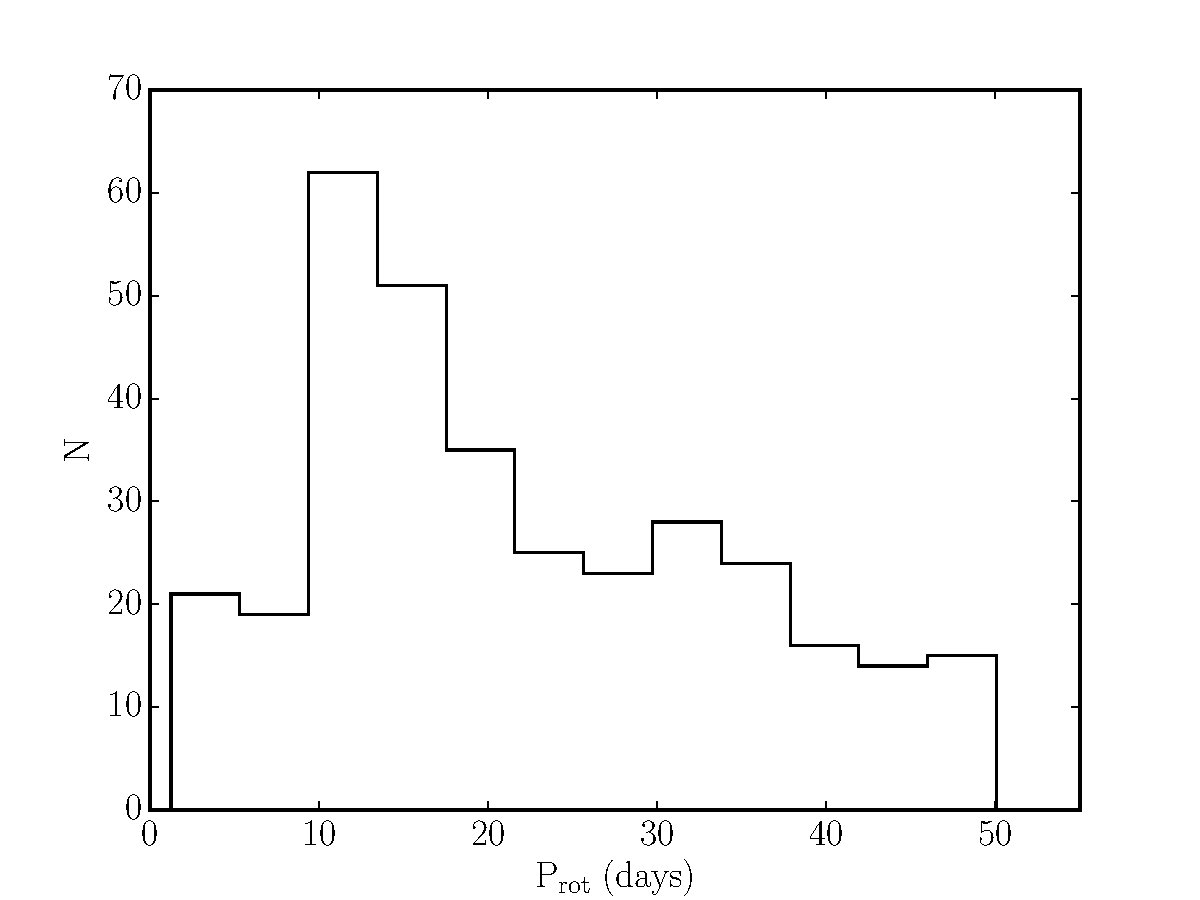
\includegraphics[width=6in, clip=true]{figures/acf_compare_noise-free_hist.pdf}
% \caption{A histogram of the rotation periods used to generate the simulated
% light curves in \citet{aigrain15}.}
% \label{fig:period_hist}
% \end{center}
% \end{figure}

\begin{figure}
\begin{center}
% 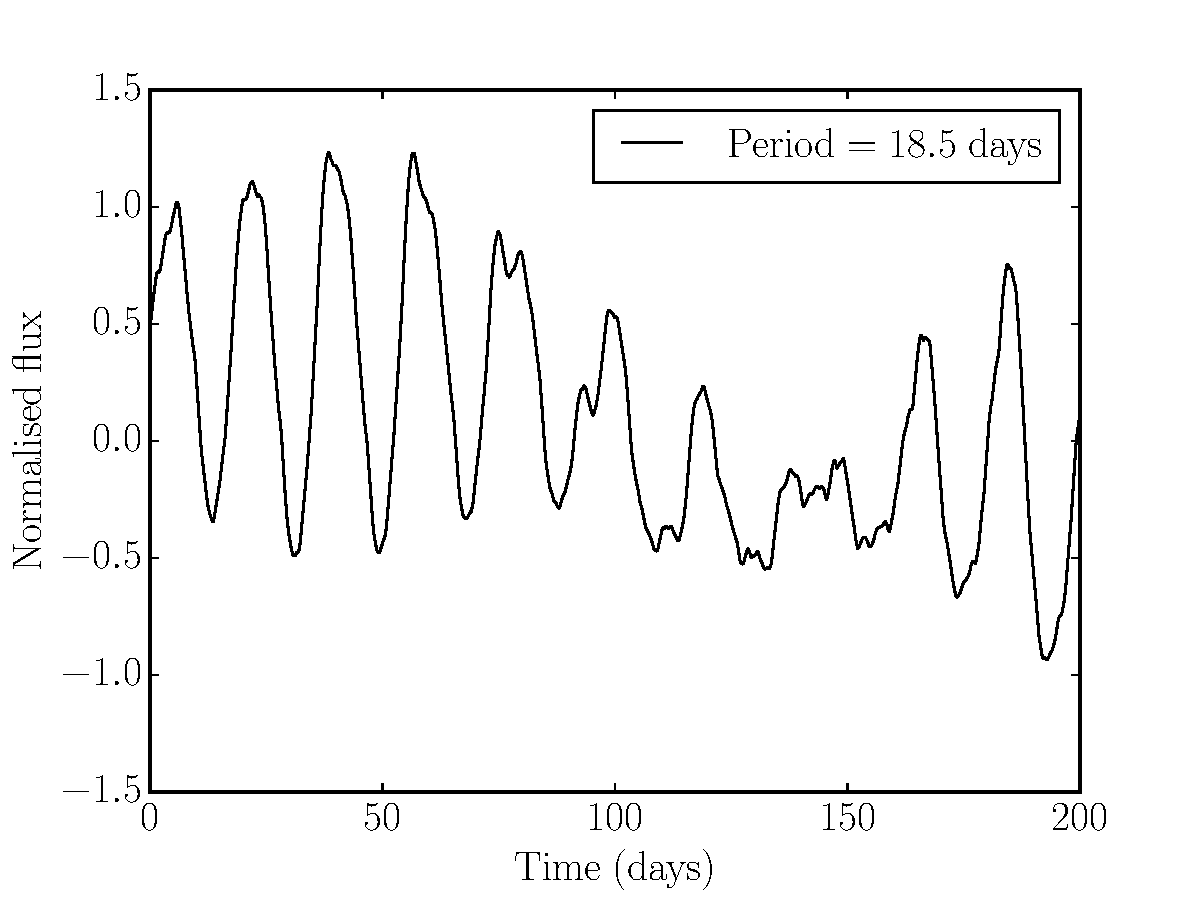
\includegraphics[width=6in, clip=true]{figures/noise-free_lc.pdf}
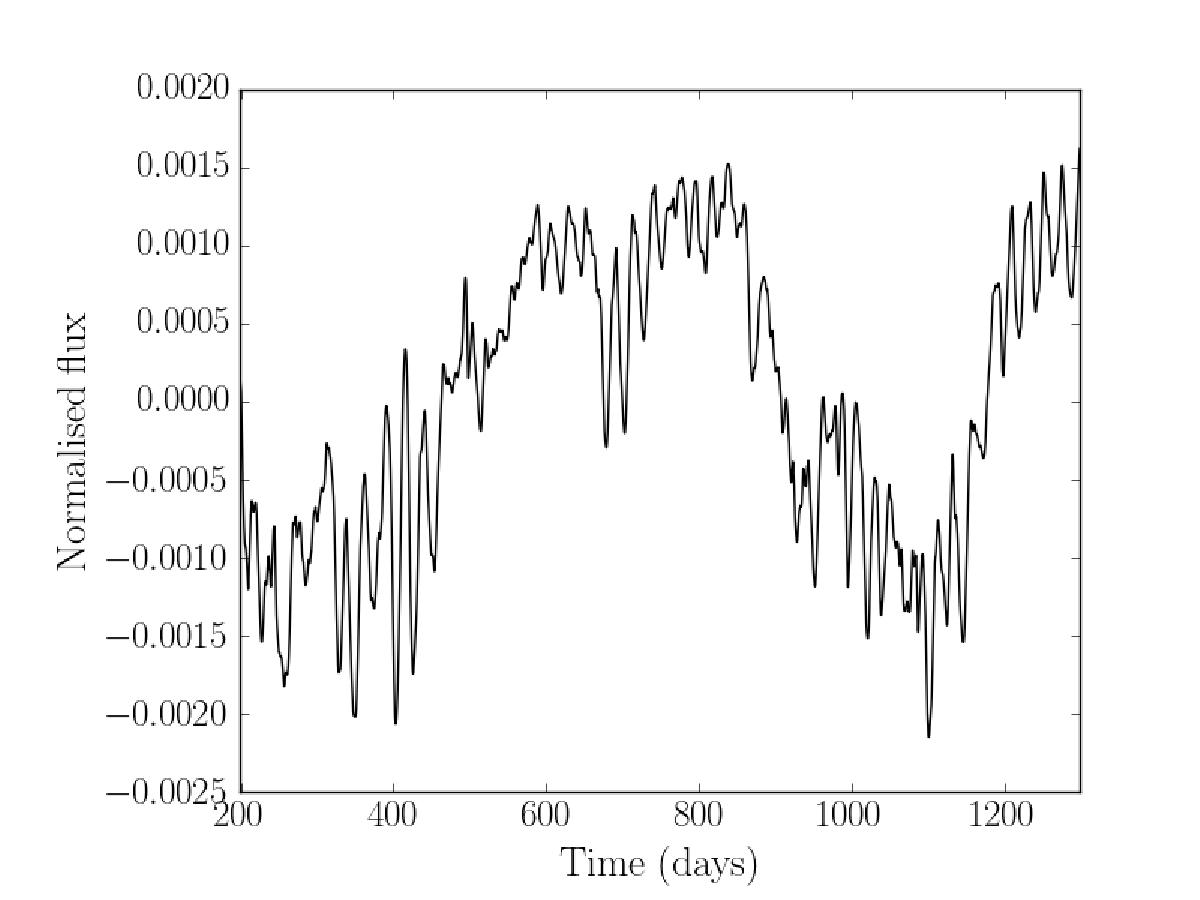
\includegraphics[width=6in, clip=true]{figures/thesis_plot.pdf}
\caption[A simulated light curve.]
{An example simulated, noise-free light curve. This `star' has a
rotation period of 17.4 days.}
\label{fig:noise-free_lc}
\end{center}
\end{figure}

Initial tests were conducted on noise-free light curves, in order to provide
proof-of-concept.
We attempted to recover the rotation periods of these \nlightcurves\ light
curves
% , both with and without noise, (\ie before {\it and} after being injected
% into \kepler light curves)
using three rotation period recovery methods: the ACF method, the LS
periodogram method and the GP method.

\subsection{ACF}

We calculated an ACF for each light curve using the method of
\citet{Mcquillan2013}.
In this method, an ACF is calculated for each light curve and smoothed by
convolving with a Gaussian with $\sigma=9$ days.
A rotation period is estimated as the lag-time of the first peak in the ACF,
unless the second peak is larger in which case {\it that} lag-time is
interpreted as the true period.
The second peak in an ACF can be larger than the first if there are two active
regions at or near opposite longitudes on the surface of the star---this would
produce a light curve with two dips per rotation period.
% By extension, if three active longitudes existed at 60$^\circ$ separations on
% the stellar surface, the first peak in the ACF may be at one third of the true
% rotation period and so on.
An example ACF of the light curve in figure~\ref{fig:noise-free_lc} is shown
in figure \ref{fig:ACF_example}.

\begin{figure*}
\begin{center}
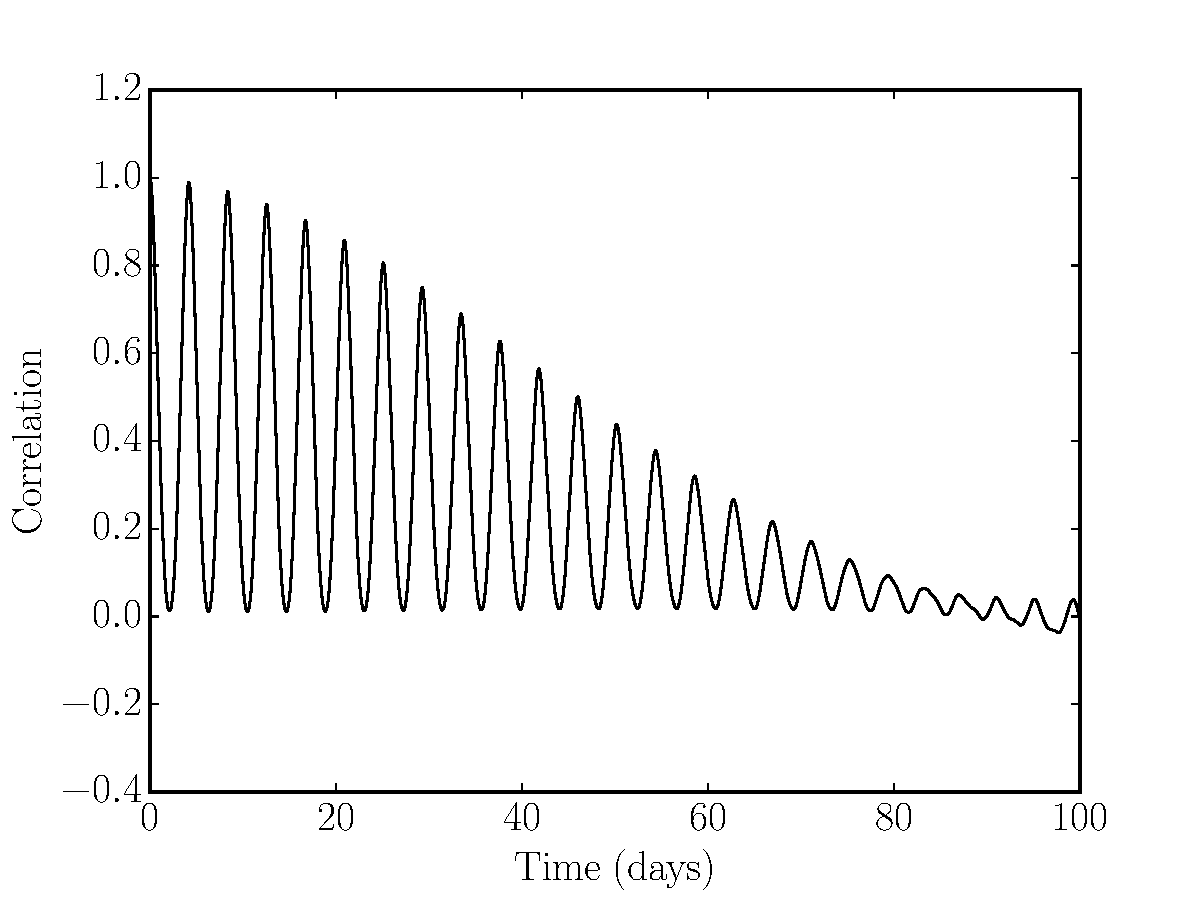
\includegraphics[width=6in, clip=true]{figures/noise-free_acf.pdf}
\caption[An ACF of a simulated light curve.]
{The autocorrelation function of the simulated, noise-free light
curve depicted in figure \ref{fig:noise-free_lc}.}
\label{fig:ACF_example}
\end{center}
\end{figure*}

The ACF method has proven to be extremely useful for measuring rotation
periods.
The catalogue of rotation periods of \Kepler\ stars provided in
\citet{Mcquillan2013} has been widely used by the community and has provided
ground-breaking results for stellar and exoplanetary science.
The results of the ACF method as tested in \citet{Aigrain2015} were positive
(see, for example their figure 8) as it produced a large number of accurate
rotation period measurements.
Another advantage of the ACF method is that it is conveniently fast to
implement.

We applied the ACF method to our sample of \nlightcurves\ noise-free,
simulated light curves.
Periods measured using the ACF method are plotted against the original
rotation period values used to generate the light curves in figure
\ref{fig:compare_noise_free}.
% 73\% of the injected rotation periods were recovered with a value lying
% within 10\% of the truth and 83\% within 20\%.
A noteworthy feature of this figure is that many of the points fall below the
$x=y$ line, \ie\ the recovered rotation periods are a little shorter than the
true periods.
We believe this is a feature of the peak position measurement method that is
performed on the ACF.
ACFs of stellar light curves can be roughly described as a cosine function
super-imposed on top of a decaying exponential.
In such a function the peak positions can be shifted towards the left--the
short period end--because the decaying exponential raises the left side of
each peak more than the right.
It is possible to model this effect of course, however the standard practice
is to simply measure the peak position without taking it into account.
We are still investigating the origin and implications of this effect.
% To demonstrate that this effect reproduces the underestimated periods seen in
% figure \ref{fig:compare_noise_free}, we simulated 1000 ACFs by generating
% cosine plus exponential functions with a range of periods, decay timescales
% and relative amplitudes.
% The measured position of the first peak in each simulated ACF is compared to
% the true position in figure \ref{fig:exp_sine_test}.
% The same underestimation of the peak position is apparent in this figure.
% Dashed lines show harmonics of $2P_{\mathrm{rot}}$ and $1/2P_{\mathrm{rot}}$.
% In several cases, twice the true rotation period is measured.
% The RMS of residuals is 1.59 days.

% \begin{figure*}
% \begin{center}
% 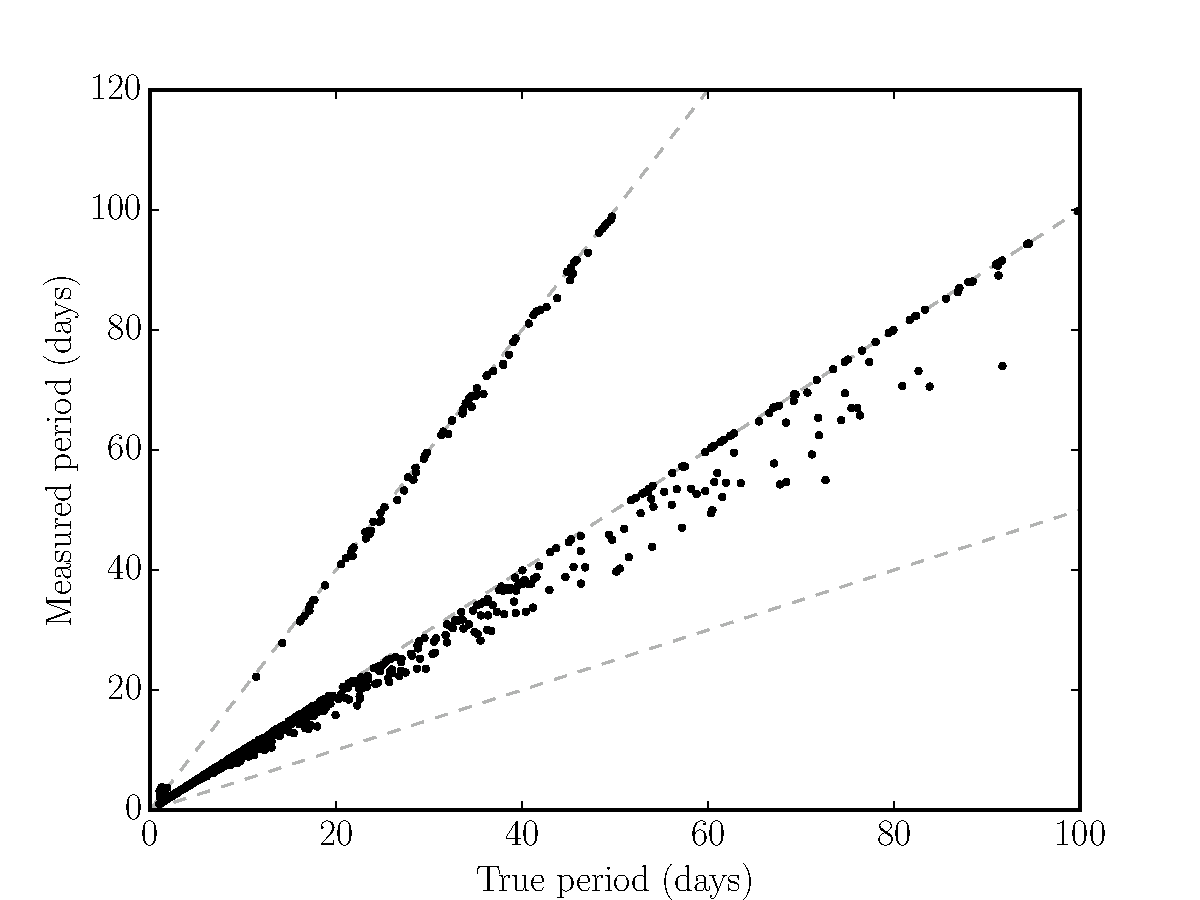
\includegraphics[width=6in, clip=true]{figures/exp_sine_test.pdf}
% \caption[A flaw in the ACF method.]
% {Recovered peak position as a function of the `true' period used to
% generate simulated ACFs. In many cases the position is measured short-wards of
% the truth, as also seen in figure \ref{fig:compare_noise_free}. The dashed
% lines are at $x=2x$, $x=x$ and $x=\frac{1}{2}x$.}
% \end{center}
% \end{figure*}
% \label{fig:exp_sine_test}

\begin{figure*}
\begin{center}
% 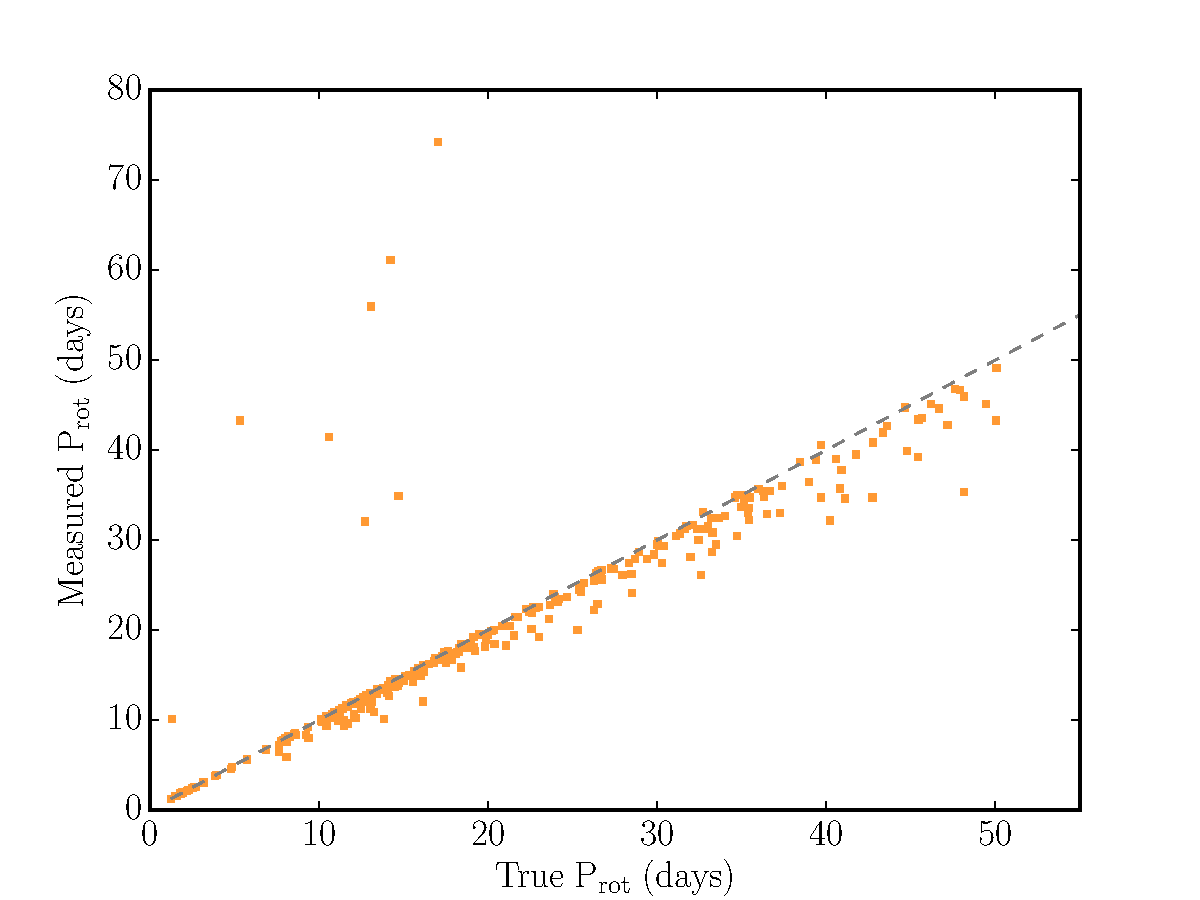
\includegraphics[width=6in, clip=true]{figures/acf_compare_noise-free.pdf}
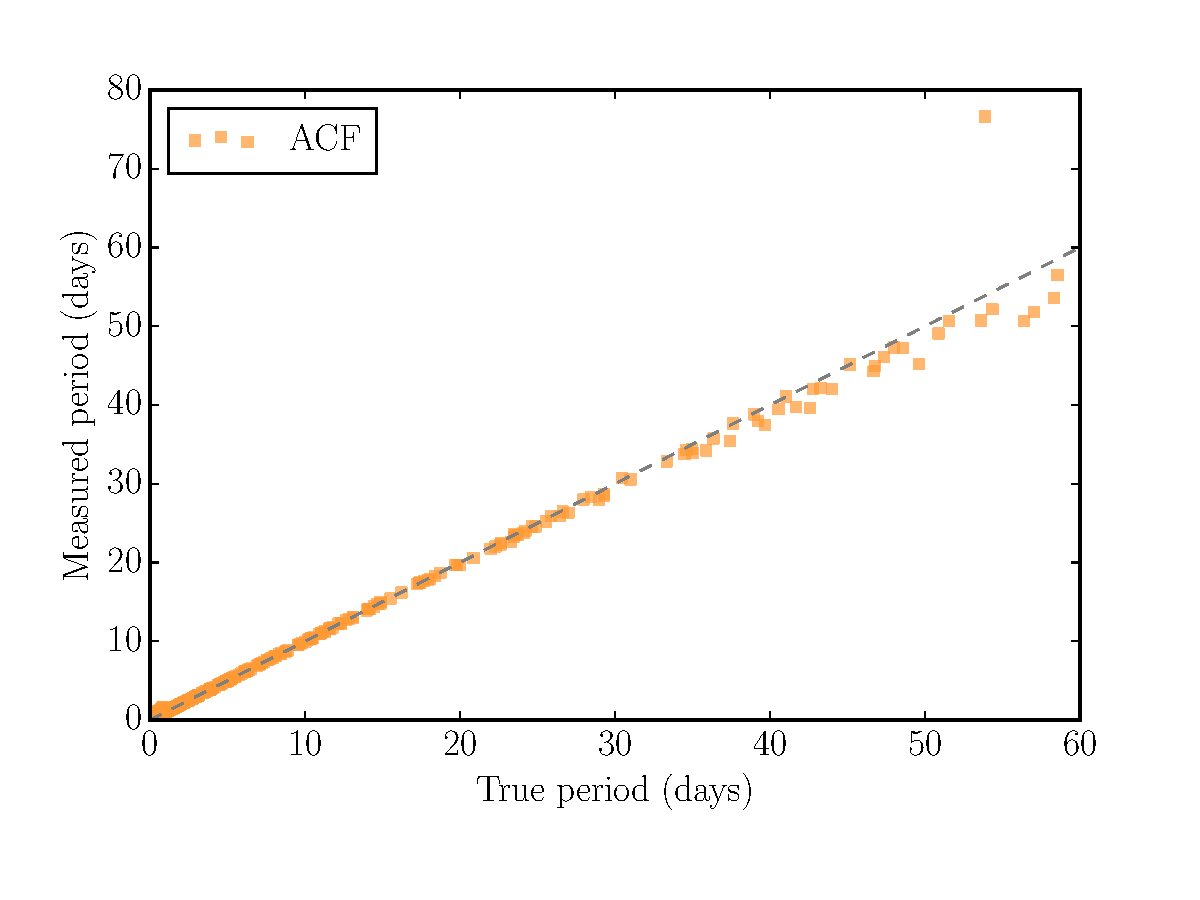
\includegraphics[width=6in, clip=true]{figures/compare_acf.pdf}
\caption[ACF results.]
{Rotation periods measured using the ACF method as a function of the
`true' period used to generate \nlightcurves\ simulated, noise-free light
curves.}
\label{fig:compare_noise_free}
\end{center}
\end{figure*}

\subsection{The sine-fitting periodogram method}

For each simulated light curve, a Lomb-Scargle (LS) periodogram
\citep{Lomb1976, Scargle1982} was computed over a grid of 10,000 periods,
evenly spaced in frequency, between 1 and 100 days.
The period of the highest peak in the periodogram was adopted as the rotation
period.
The resulting recovered rotation periods are plotted as a function of the true
periods in figure \ref{fig:pgram_compare_noise_free}.
These recovered rotation periods are in general more accurate than the ACF
results: they do not systematically over or under predict rotation period.
They are however less precise than the ACF results---the 8.03 day RMS of
residuals is five times larger.
% We believe that the unsuccessful recoveries occurring preferentially for
% shorter rotation periods are produced by additional, longer timescale
% variations in some of the light curves.
% Specifically, by fluctuations produced by changes in the total spot coverage
% on the stellar surface.
% These fluctuations can occasionally be larger in magnitude than those produced
% by the rotational signal itself and are present in the majority of outlying
% light curves that occupy the top left of figure
% \ref{fig:pgram_compare_noise-free}.

\begin{figure*}
\begin{center}
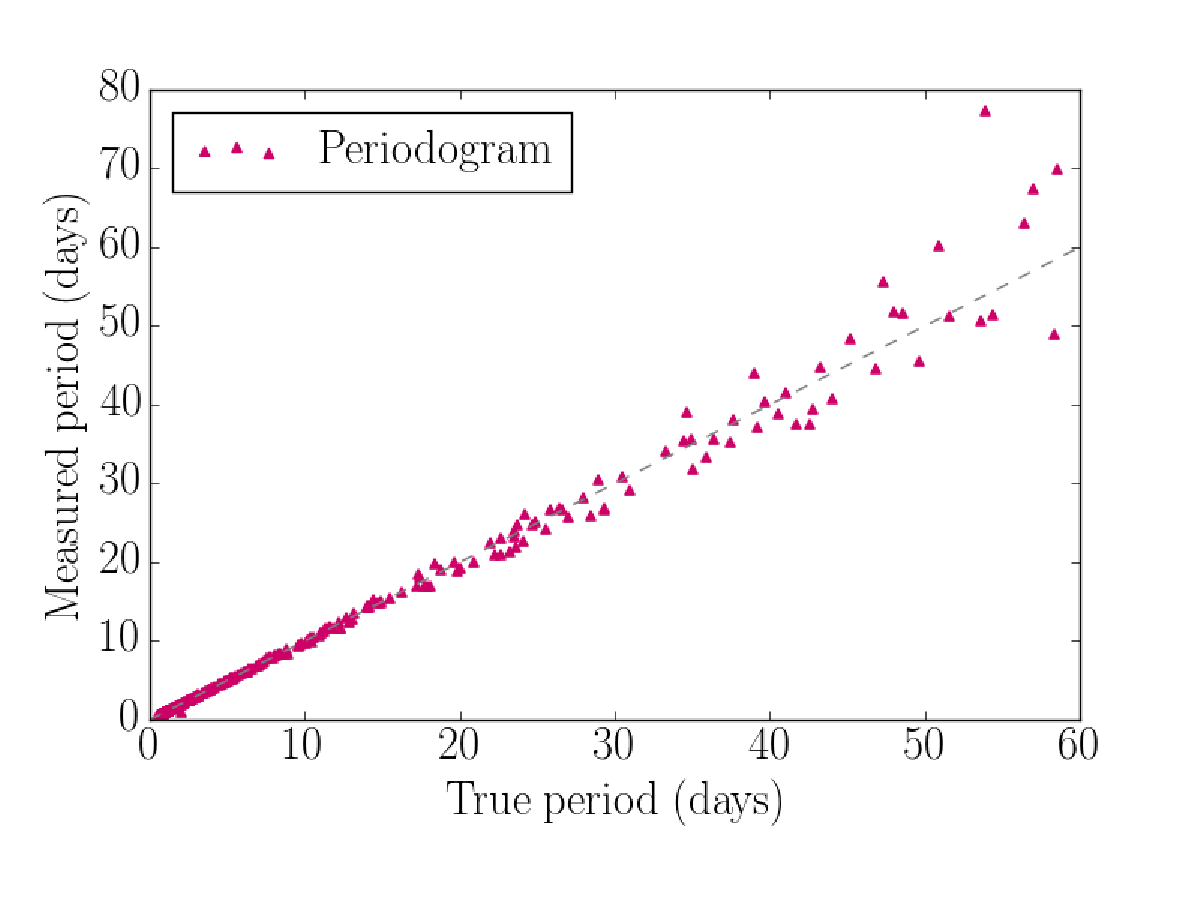
\includegraphics[width=6in, clip=true]{figures/compare_pgram.pdf}
\caption[LS periodogram results.]
{Rotation periods measured using the LS periodogram method as a
function of the `true' rotation period used to generate \nlightcurves\
simulated light curves.}
\label{fig:pgram_compare_noise_free}
\end{center}
\end{figure*}

\subsection{The GP method}

In order to recover the rotation periods of the simulated light curves using
Gaussian processes, we sampled the posterior PDFs of the kernel
hyperparameters described in equation \ref{eq:QP}.
The likelihood function for a GP is similar to the simple Gaussian likelihood
function that is used for optimisation problems where the uncertainties are
Gaussian and uncorrelated.
The latter can be written
\begin{equation}
\ln \mathcal{L} = -\frac{1}{2}\sum_{n=1}^N\frac{(y_n-\mu)^2}{\sigma_n^2}
    - \frac{N}{2}\ln(2\pi\sigma_n^2),
\end{equation}
\label{eq:chi2}
where $y_n$ are the data, $\mu$ is the mean model and $\sigma_n$ are the
Gaussian uncertainites on the data.
The equivalent equation in matrix notation is
\begin{equation}
\ln \mathcal{L} = -\frac{1}{2}\bf{r}^T\bf{C}^{-1}\bf{r}-\ln|\bf{C}|
    + \mathrm{constant},
\end{equation}
\label{eq:lhf1}
where $\bf{r}$ is the vector of residuals and $\bf{C}$ is the covariance
matrix,
\begin{eqnarray}
	\mathbf{C} &=& \left (\begin{array}{cccc}
	\sigma^2_1 & \sigma_{2, 1} & \cdots & \sigma_{N, 1} \\
	\sigma_{1, 2} & \sigma^2_2 & \cdots & \sigma_{N, 2} \\
    && \vdots & \\
	\sigma_{1, N} & \sigma_{2, N} & \cdots & \sigma^2_N
\end{array}\right )
\end{eqnarray}
In the case where the uncertainties are uncorrelated, the noise is `white',
(which is a frequent assumption made by astronomers and is sometimes
justified) and the off-diagonal elements of the covariance matrix are zero.
However, in the case where there is evidence for correlated
`noise'\footnote{In our case the `noise' is actually the model!}, as in the
case of \Kepler\ light curves, those off-diagonal elements are non-zero.
With GP regression, a covariance matrix generated by the kernel function,
${\bf K}$ replaces ${\bf C}$ in the above equation.
Incidentally, this approach is the reverse of the regression techniques
usually employed by astronomers.
In most problems in astronomy one tries to infer the parameters that describe
the mean model and, if correlated noise is present, to marginalise over that
noise.
Here, the parameters describing the correlated noise are what we are
interested in and our mean model is simply a straight line at $y=0$.

One could either maximise this likelihood function in order to find the
best-fit hyper-parameters of the covariance kernel function or, as in our
approach, sample from the posterior PDFs of the hyper-parameters.
The advantage of the maximum-likelihood method is that the best-fit parameters
will be found much faster, but the uncertainities on the rotation period
will not be constrained.
In order to measure accurate uncertainties, the posterior PDFs of the
parameters must be explored.
Since obtaining accurate uncertainties on rotation periods is one of our main
motivations for this method, we use MCMC despite the added computational
expense.

We use the ACF period as an initial guess for the rotation period (this
decision is discussed further in section \textsection \ref{sec:discussion}).
We use a uniform prior over rotation period with bounds described below and
assert that the covariance decay timescale parameter, $l$ must be greater than
the rotation period.
This represents our assumption that the evolution timescale of active regions
is greater than stellar rotation periods.
This assumption may be more valid for late spectral types---hot stars have
smaller active regions which are likely to be shorter-lived.
For the remaining hyperparameters we use the following initial values and
log-uniform prior distributions:
\begin{eqnarray}
 	&	A_{initial} = e^{-5}, \sim \exp(U[-20:20]) \\ \nonumber
 	&	l_{initial} = e^{7}, \sim \exp(U[-20:20]), l<P \\ \nonumber
 	&	\Gamma_{initial} = e^{0.6}, \sim \exp(U[-20:20]) \\ \nonumber
 	&	\sigma_{initial} = e^{-16}, \sim \exp(U[-20:20]) \\ \nonumber
 	&	P_{initial} = P_{ACF}, \sim U([1 - 0.4]P_{ACF}<P_{ACF}<[1 +
0.4]P_{ACF}).
 \end{eqnarray}
 \label{eq:initialisation}
$\sigma$ is an additional white noise term added to the diagonal elements of
the covariance matrix. It is the fraction by which the observational
uncertainties have been underestimated.
If the errorbars reported on the data are too small, this parameter will be
non-zero.
In practice this parameter should always be non-zero when performing GP
regression.
This is because the covariance matrix must be positive definite, however
matrix inversion performed using most solvers is approximate, not exact,
therefore slight deviations from positive definitism can arise.
Including a small amount of extra variance in the model allows enough
flexibility that the matrix inversion algorithms do not run into numerical
issues.

We subsampled the light curves in order to reduce computation time.
The subsampling is altered for each light curve and depends, again, on the ACF
period estimate.
We found that retaining only 20 data points per rotation period, based on the
ACF period estimate, significantly reduced computation time whilst maintaining
performance.
The {\tt george} \citep{George} python package was used to implement the GP
model which uses the fast matrix solver, HODLR \citep{Ambikasaran2014}.
Matrix operations performed with HODLR scale as $N \log ^2 (N)$, where $N$ is
the number of data points.
We used {\tt emcee} \citep{Foreman-Mackey2013}, an affine invariant ensemble
sampler to explore the posterior PDFs of the model parameters.
The rotation period was taken as the median value of the posterior PDF.
The resulting measured rotation periods are compared to the true rotation
periods in figure \ref{fig:GP_compare_noise_free}.
The root-mean-square (RMS) of residuals for the GP results is 0.26 days.
The results of all three methods are plotted on the same axes in figure
\ref{fig:compare_noise_free}.

% The subsampling reduces computation time simply by contracting the data

\begin{figure*}
\begin{center}
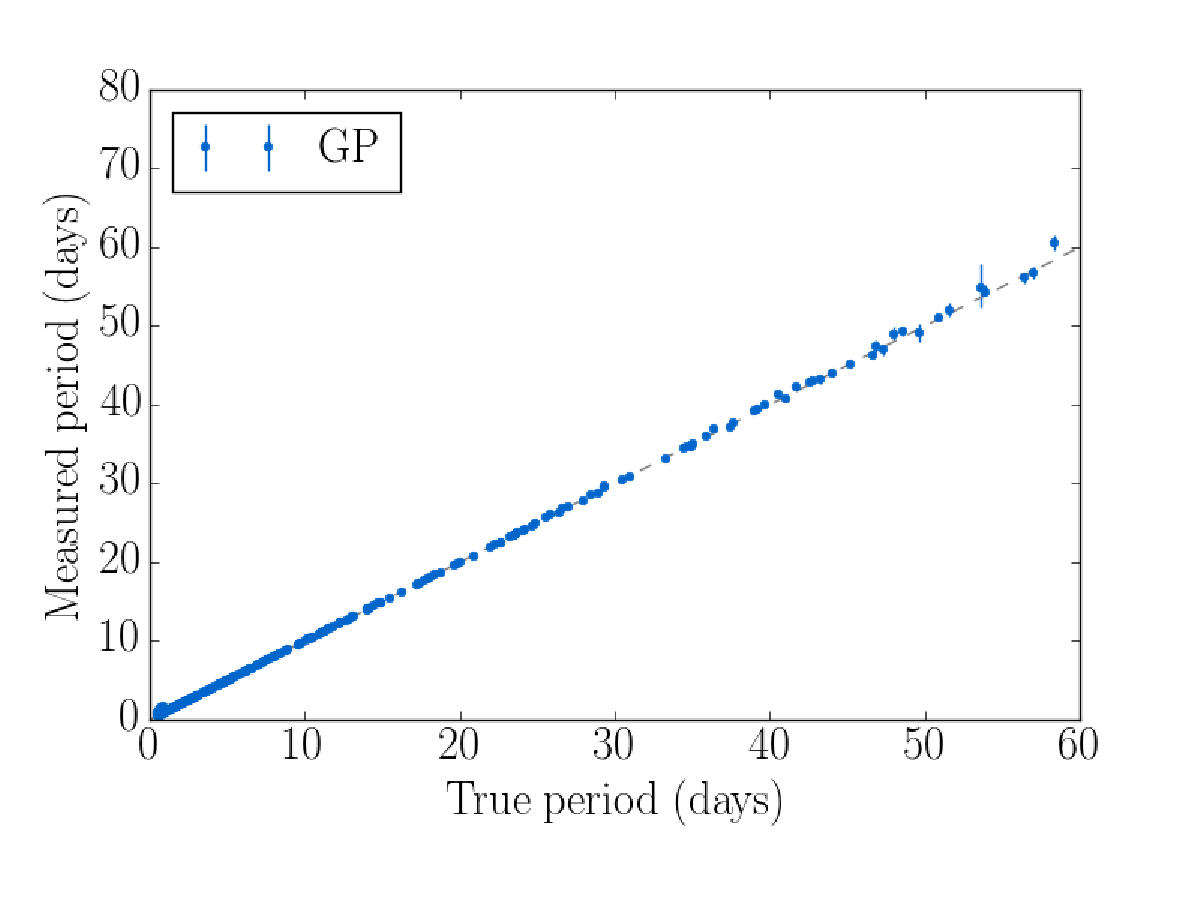
\includegraphics[width=6in, clip=true]{figures/compare_gp.pdf}
\caption[GP results.]
{Measured vs true rotation period for \nlightcurves\ simulated light
curves using the GP method.}
\label{fig:GP_compare_noise_free}
\end{center}
\end{figure*}

\begin{figure*}
\begin{center}
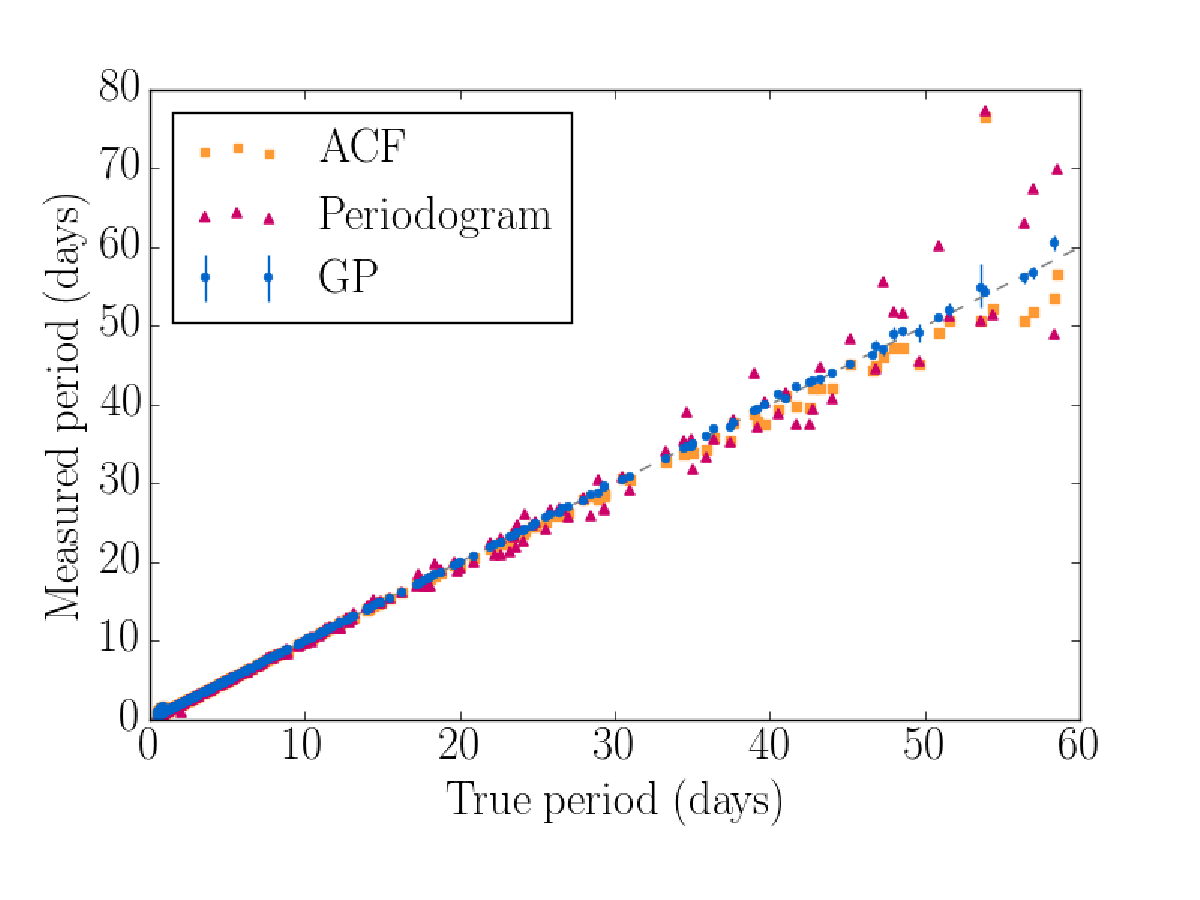
\includegraphics[width=6in, clip=true]{figures/compare2.pdf}
\caption[All results.]
{Measured vs true rotation period for \nlightcurves\ simulated light
curves from the three different methods described in the text.}
\label{fig:compare_noise_free}
\end{center}
\end{figure*}

The marginal posterior distributions of the QP kernel hyperparameters for an
example noise-free light curve  with a 14.4 day rotation period, are shown in
figure \ref{fig:gp_posteriors}.
The light curve itself with the best fit GP model is shown in figure
\ref{fig:demo_lc_GP}.

\begin{figure*}
\begin{center}
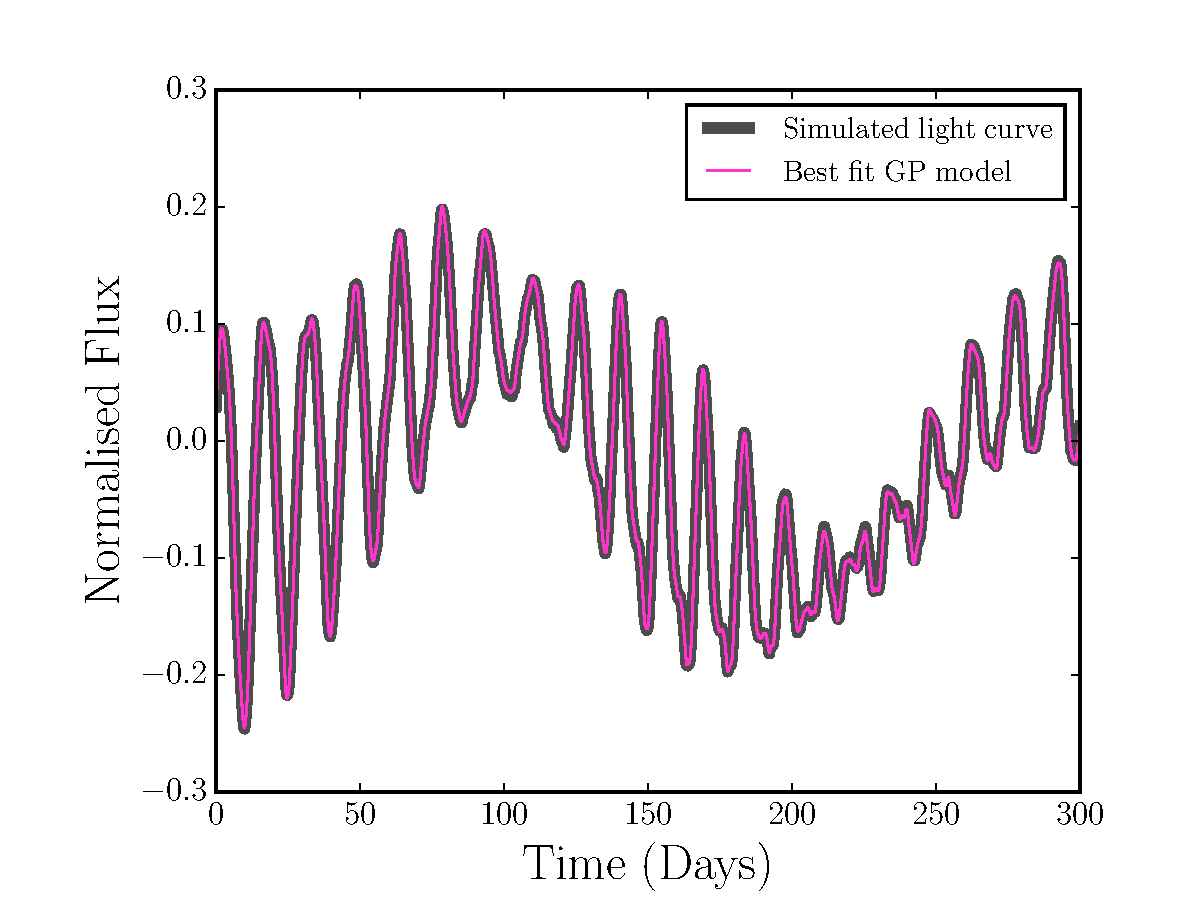
\includegraphics[width=6in, clip=true]{figures/demo_lc_GP.pdf}
\caption{A simulated light curve with a rotation period of 14.4 days.
The pink curve shows the GP model with the best-fit parameters.
The marginal posteriors of the GP hyper-parameters used to produce this fit
are shown in figure \ref{fig:gp_posteriors}.}
\label{fig:demo_lc_GP}
\end{center}
\end{figure*}

\begin{figure*}
\begin{center}
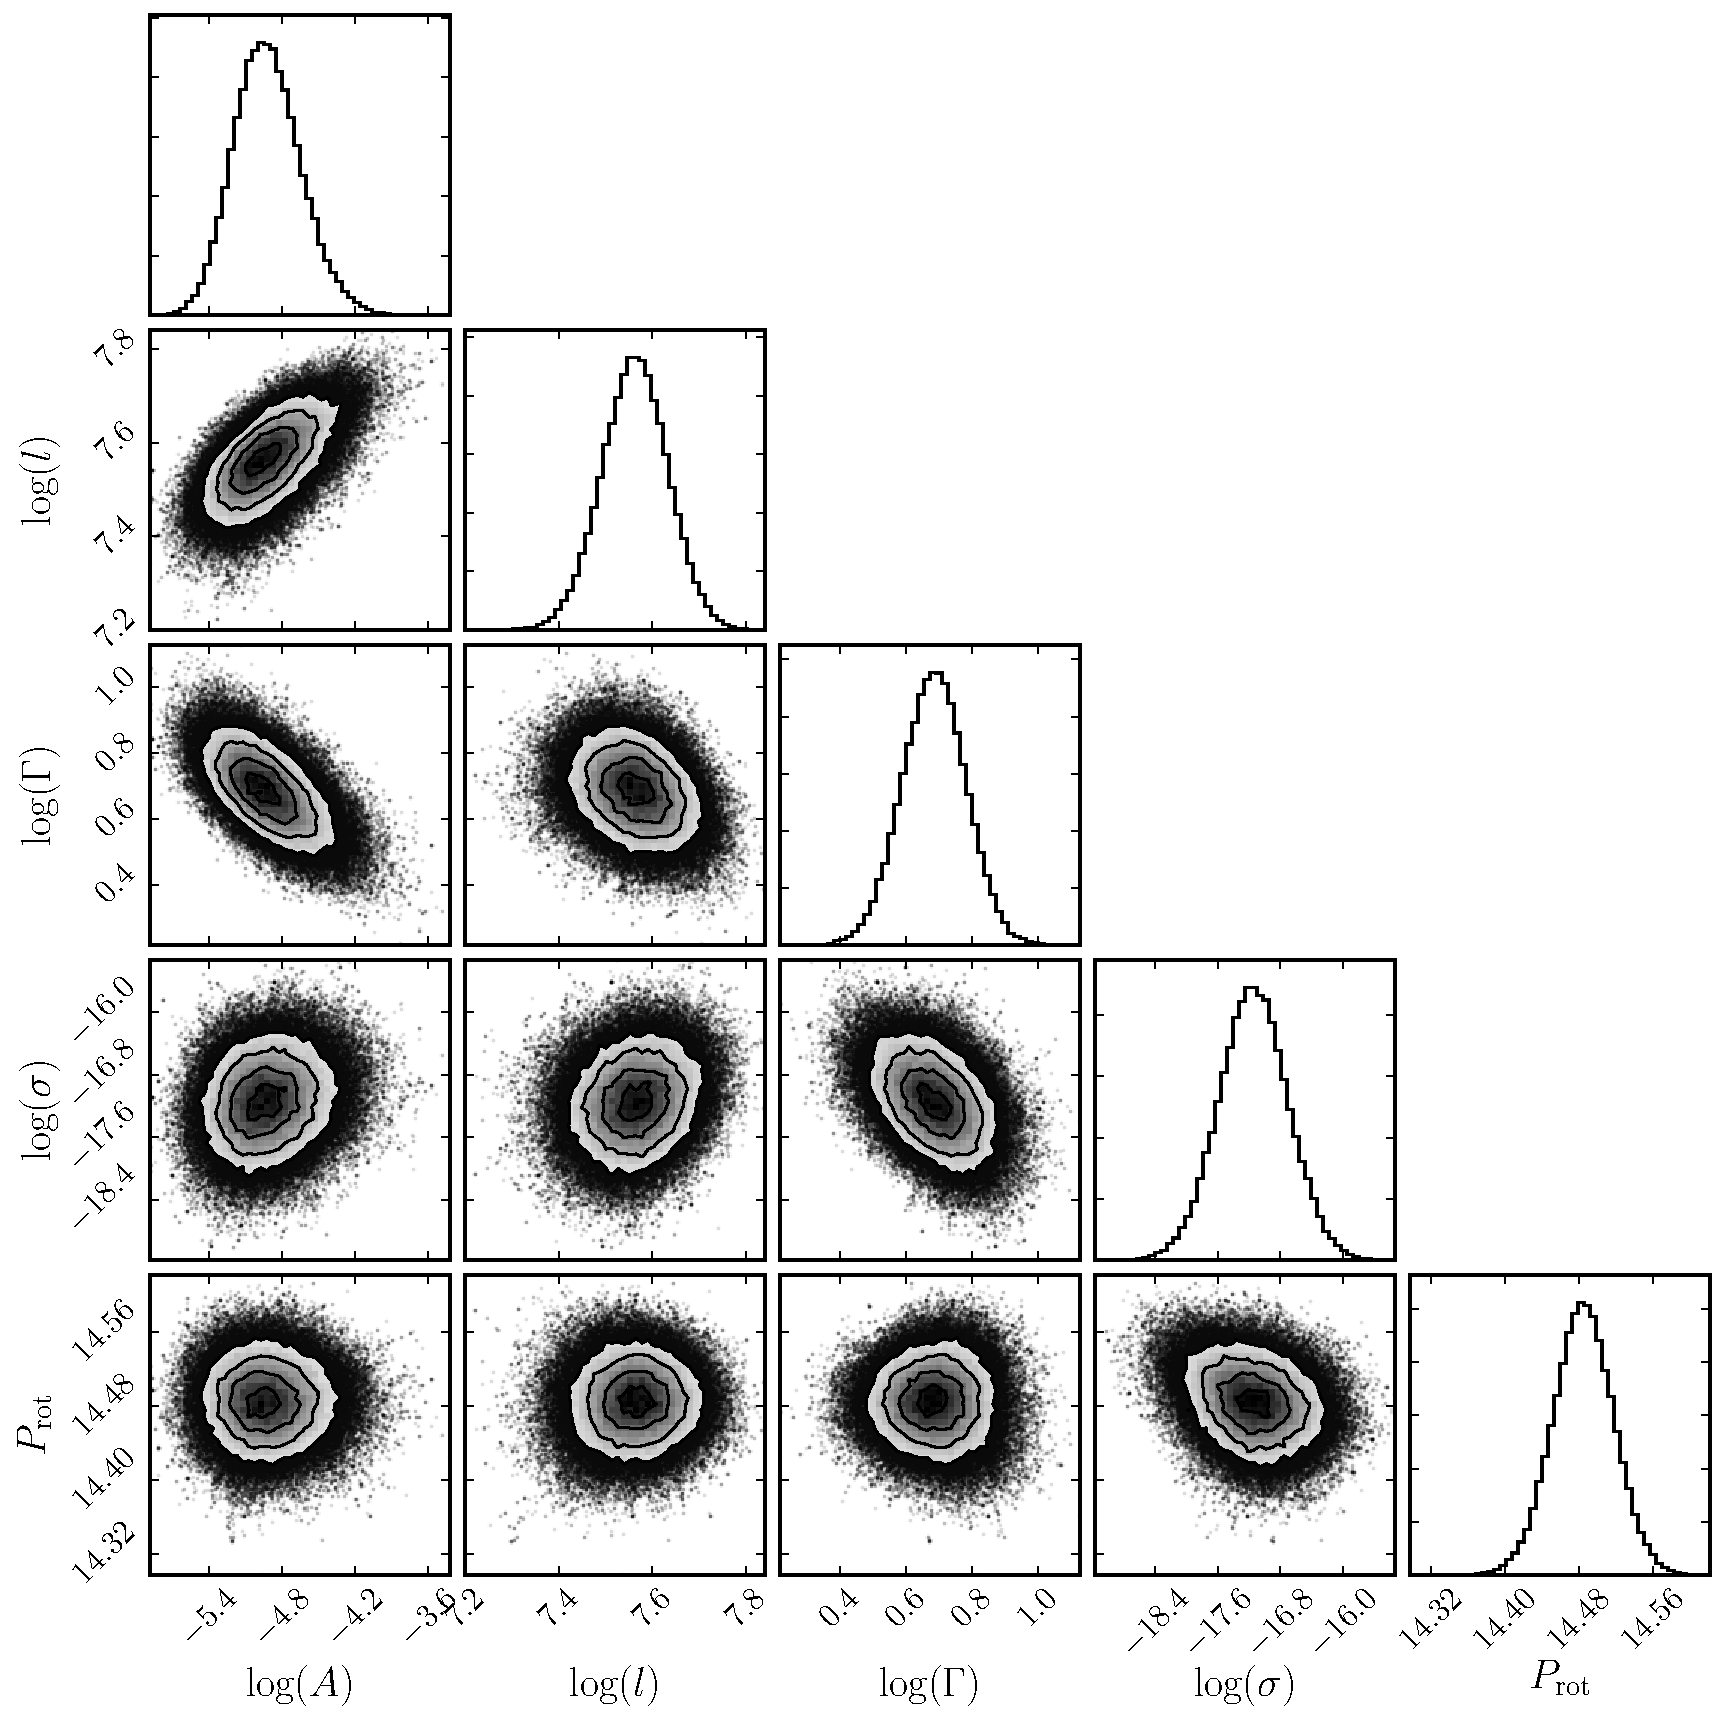
\includegraphics[width=6in, clip=true]{figures/demo_triangle.pdf}
\caption{Marginal posterior PDFs of the QP GP model parameters. $\sigma$ is an
additional white noise term added to the diagonal elements of the covariance
matrix. It is the fraction by which the observational uncertainties have been
underestimated. If the errorbars reported on the data are too small, this
parameter will be non-zero. Since this light curve was simulated without
noise, this parameter is very close to zero.
The true rotation period of this star is 14.4 days.}
\label{fig:gp_posteriors}
\end{center}
\end{figure*}

\subsection{Real \kepler\ data}

The noise-free light curves were injected into real \kepler\ light curves in
order to test the performance of the GP method in a realistic case.
Ideally, simulated light curves would have been injected into the \kepler\
pixel-level data, then the same detrending method that is applied to the
\kepler\ light curves would be applied to these light curves before attempting
to measure rotation periods for these stars.
However, since this work is designed to be more of a demonstration of the
overall efficacy of the GP periodogram, rather than the development of a
\Kepler\ specific method, this is beyond the scope of our demonstrations.

Unfortunately, automating the GP method so that it can run on large numbers of
real \kepler\ light curves is difficult.
The added noise reduces the acceptance fraction within the MCMC chains,
significantly increasing the required time for convergence.
Despite this, the method works well on individual targets where chains can be
run for a long time and subsampling can be reduced.
We used a simulated, noisy light curve from \citet{Aigrain2015} that was
generated by injecting a noise-free simulation into a real \kepler\ light
curve in order to preserve realistic \kepler\ noise properties.

\kepler\ light curves are big data and extracting the maximum amount of
information from them requires either large numbers of CPU hours, or using
work-arounds.
One feature of \kepler\ light curves that works to our advantage is that they
are naturally broken up into smaller time units by quarterly (three month)
breaks.
Splitting the data set into quarters, rather than modelling the entire time
series contiguously speeds up the computation time as inverting several
small matrices is faster than inverting one large one.
The \kepler\ quarter divisions are natural places to split the time series
because the spacecraft rotates by ninety degrees every quarter (three months),
placing each star on a new CCD module.
Pixel response functions and background flux differs from pixel-to-pixel and
module-to-module, so noise properties of \kepler\ light curves change every
quarter.
Additionally, changes in the spacecraft's orientation and position during
quarterly re-pointings temporarily affect the temperature of the CCD,
producing systematic features in the light curves at the start of some
quarters.
We model each quarter separately but the parameters of the GP kernel function
are global, {\it i.e.} we do not use a separate period parameter for each
quarter---there is just one period parameter for an entire light curve.
It would be possible to model the time series with a mixture of some global
parameters and some quarter-specific parameters, for example one might expect
that the amplitude of covariance, $A$ or white noise level, $\sigma$ to vary
on a quarterly basis.
However, since there are seventeen quarters this would lead to thirty-seven
parameters, and in the interest of minimising computation time (adding
parameters leads to longer MCMC burn in and convergence time), we choose to
use global parameters only.
Unfortunately, the application of this method to noisy test cases is still
under development and cannot provide results here.
We hope to develop this method further and apply it to real light curves in
the near future.

% The marginal posterior distributions of the QP kernel hyperparameters for an
% example noisy light curve  with a ... day rotation period, are shown in
% figure \ref{fig:gp_posteriors}.
% The light curve itself with the best fit GP model is shown in figure
% \ref{fig:demo_lc_GP}.

% \begin{figure*}
% \begin{center}
% 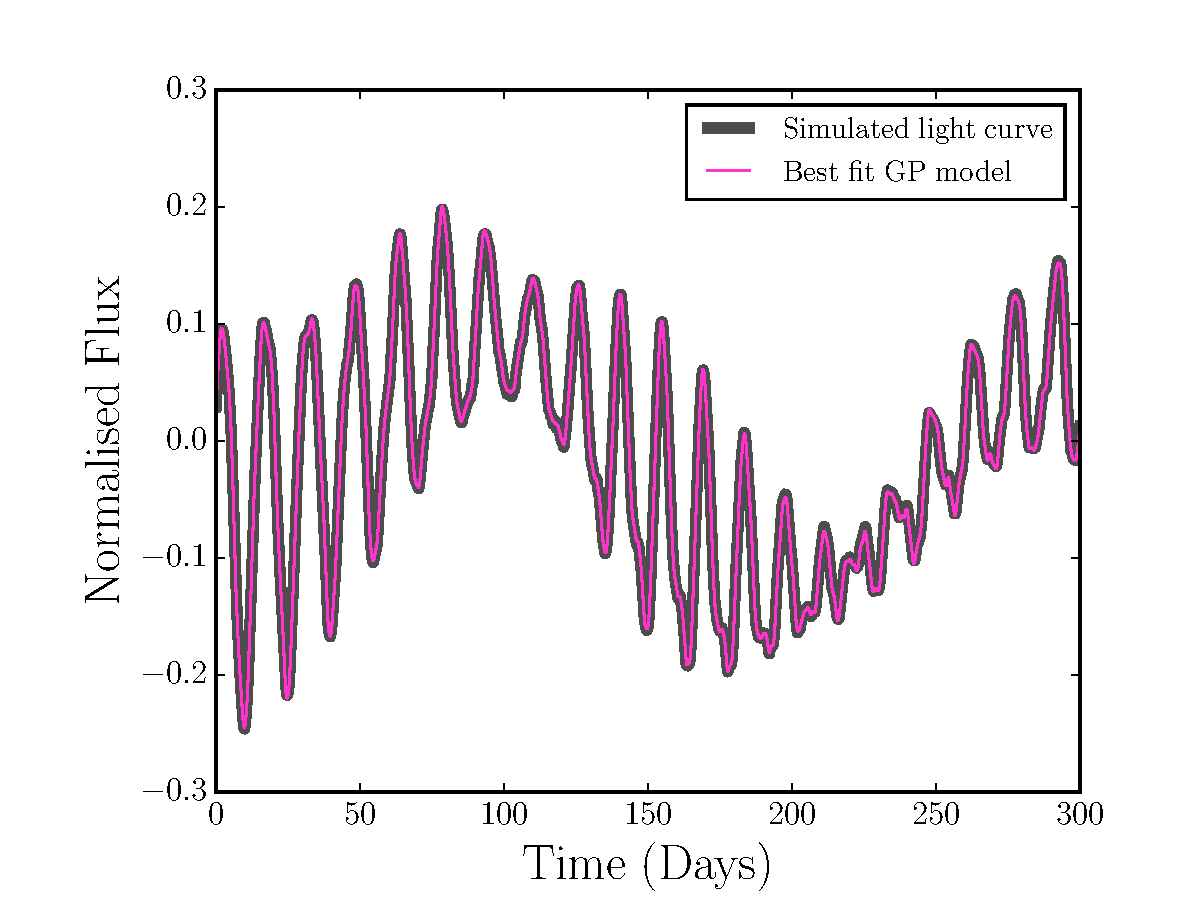
\includegraphics[width=6in, clip=true]{figures/demo_lc_GP.pdf}
% \caption{A simulated light curve with a rotation period of 14.4 days.
% The pink curve shows the GP model with the best-fit parameters.
% The marginal posteriors of the GP hyper-parameters used to produce this fit
% are shown in figure \ref{fig:gp_posteriors}.}
% \label{fig:demo_lc_GP}
% \end{center}
% \end{figure*}

% \begin{figure*}
% \begin{center}
% 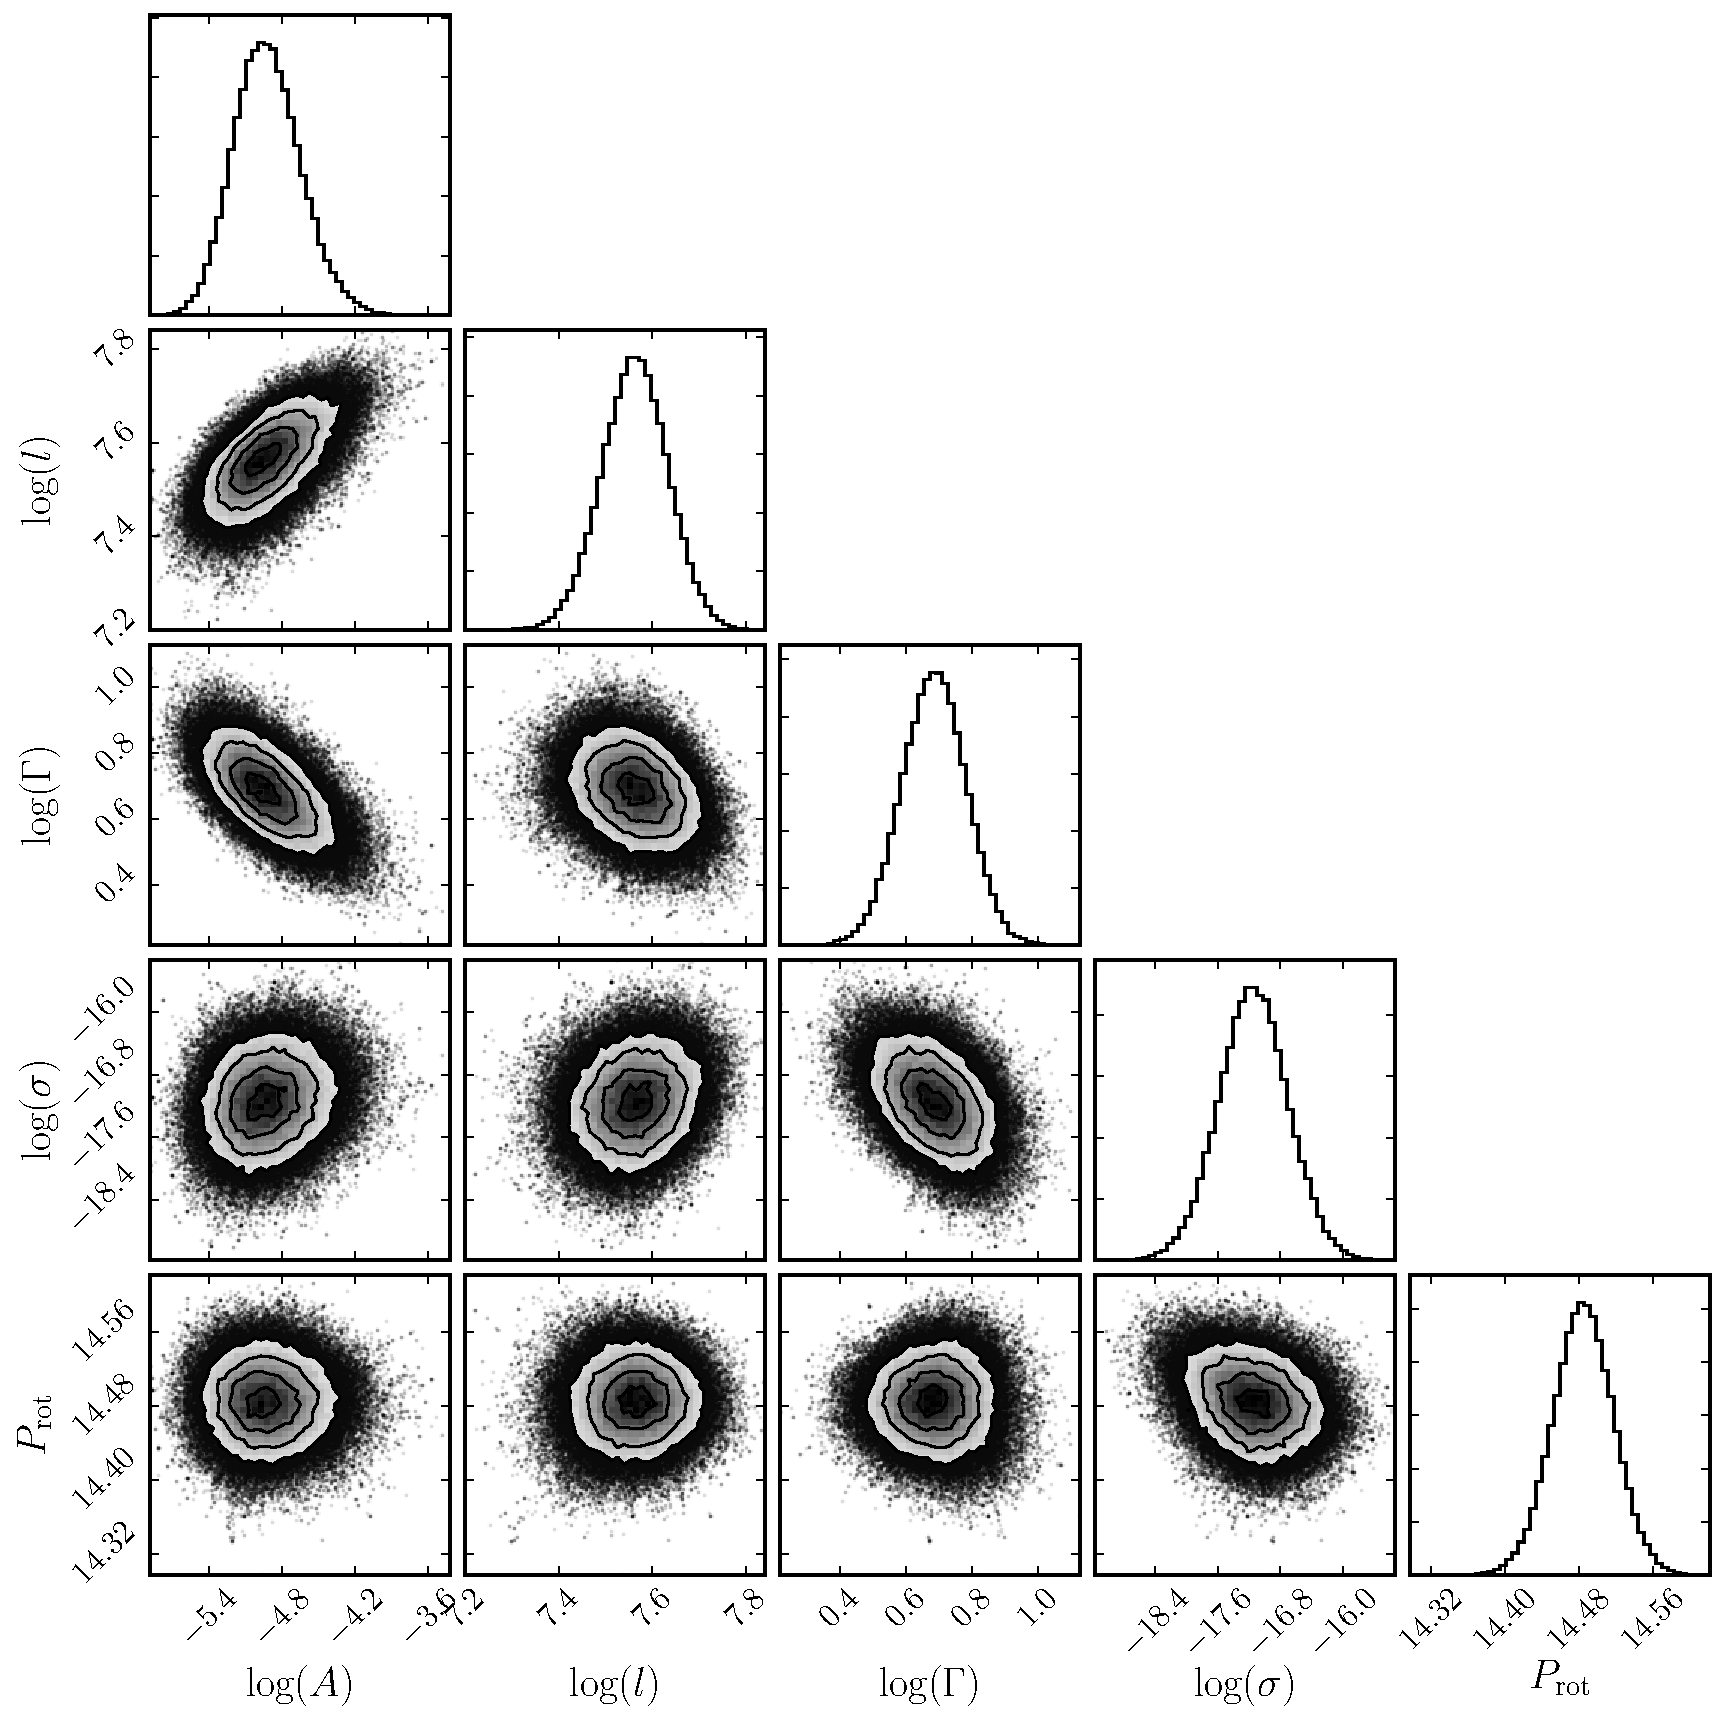
\includegraphics[width=6in, clip=true]{figures/demo_triangle.pdf}
% \caption{Marginal posterior PDFs of the QP GP model parameters. $\sigma$ is an
% additional white noise term added to the diagonal elements of the covariance
% matrix. It is the fraction by which the observational uncertainties have been
% underestimated. If the errorbars reported on the data are too small, this
% parameter will be non-zero. Since this light curve was simulated without
% noise, this parameter is very close to zero.
% The true rotation period of this star is 14.4 days.}
% \label{fig:gp_posteriors}
% \end{center}
% \end{figure*}

% \begin{figure*}
% \begin{center}
% \includegraphics[width=6in, clip=true]{figures/prediction.pdf}
% \caption{A noisy simulated light curve with a rotation period of 17.04 days.
% The blue curve shows the GP model with the best-fit parameters.}
% \end{center}
% \end{figure*}
% \label{fig:compare_noise_free}

\section{Discussion}
\label{sec:discussion}

The main drawback of the GP method is computation time.
Because GPs are so expensive to compute, it is necessary to come up with
shortcuts in order to perform inference on \kepler\ light curves, each of
which compromises accuracy.
The shortcuts that we employ here include:
\begin{itemize}
\item{Initialisation.
The choice of initial parameter values makes a difference to computation time:
the closer they are to the maximum likelihood parameters the shorter the MCMC
burn-in time.
Using the ACF period to initialise is not ideal as results will not be fully
independent of the ACF period unless MCMC chains are run for an infinitely
long time.} \item{Subsampling.
Not only is some information always lost by subsampling, but the choice of
subsampling frequency will also effect the results.
We chose to retain only 20 data points per period --- based on the ACF
period --- which, again means that our results are not independent of the ACF
results.}
\item{Priors.
We chose to use uniform, bounded priors to reduce parameter space and
therefore convergence time.
Unfortunately, if the true period lies outside the bounded region, it will
never be found.}
\end{itemize}

These shortcuts are only necessary when working with a large number of stars
(of order hundreds or thousands).
If only interested in single or small numbers of targets it may be possible to
reduce the extremity of these shortcuts or to avoid them altogether.

\subsection{The ACF method}
The main advantage of the ACF method over the GP method is speed: it is
extremely fast and therefore useful to get a quick estimate of a period.
We have demonstrated that the ACF method may produce rotation periods that are
slightly systematically biased towards lower rotation periods.
This effect comes from the process of extracting the period from the ACF
itself: typically superimposed onto a decaying exponential, that first peak in
the ACF gets shifted towards faster periods.
One may be able to get around this by modelling the ACF as a sum of a cosine
and exponential function (a similar function to GP kernel function) but
in practice ACFs tend to have a more complicated structure and it is not
possible to model them with a simple function.
This observation leads to the idea of modelling the ACF with a Gaussian
processes, which then logically progresses to a using a Gaussian process with
a Gaussian process kernel function.
Although this may be an attractive idea, in practice a GP would not
necessarily produce a positive semi-definite covariance kernel\footnote{One
that can be inverted; a necessary regression operation.}.
An alternative approach may be to correct for rotation period bias after the
peak position has been measured by inferring a correction factor.
Yet another approach could be to measure the mean separation between adjacent
peaks in the ACF: the first peak should be most strongly affected by the
exponential decay, the second peak less so, and so on.

\subsection{Initialisation}
Using the ACF to initialise the MCMC chains is not ideal because, of course,
one becomes reliant on the assumption that the ACF period is close to the true
period.
Of course, if you had infinite CPU time, this would not be a problem as you
would eventually sample the entire posterior PDF of the period parameter,
however in practice this is likely to be an issue.
The only way to get around this problem is to run the MCMC chains for as long
as possible, or, alternatively to use a sampler that is designed to move
around the parameter space much more quickly than {\tt emcee}; nested sampling
for example.
We chose to use the ACF periods rather than the periodogram periods to
initialise as, although there was some systematic bias present in these
results, that bias was small and there were fewer large outliers.

\subsection{Kernel function choice and interpretation of hyper-parameters}
The QP kernel function represents a simplistic effective model of a stellar
light curve.
It adequately describes the data, captures that all-important periodic quality
and is relatively simple, with only a few hyper-parameters.
It also satisfies the requirement to produce positive semi-definite covariance
matrices.
Whilst the QP kernel function evidently captures the periodic qualities of
light curves adequately, it is still a somewhat arbitrary choice.
Another valid choice would be a squared cosine function multiplied by a
squared exponential,
\begin{equation}
k_{i,j} = A \exp \left(-\frac{(x_i - x_j)^2}{2l^2}\right)
\cos^2\left(\frac{2\pi}{P}\right)
\end{equation}
\label{eq:cos_kernel}
This function produces a positive semi-definite matrix and has the $P$
parameter of interest.
It may in fact be even {\it more} suited to modelling stellar
light curves as it describes a Gaussian in frequency space.
It is easy to imagine a differentially rotating star with a period that is a
Gaussian in frequency space: the mean frequency would be the frequency at the
most active latitude, at or near which spots spend the majority of their time
and the tails would be occupied by spots that drift near the equator or poles.
The main difference between this cosine and the QP function is that the cosine
function allows negative covariances and the QP function does not.
Is is realistic to allow negative covariances?
In practice, the ACFs of \Kepler\ light curves often go negative.
However, many stars have two active regions on opposite hemispheres that
produce two brightness dips per rotation.
If the covariance is forced to be negative for two data points that are
separated by half a rotation period, those light curves with two peaks per
rotation period may not be well modelled.
It would be very worthwhile to test this assumption and this alternative
kernel function in future.
If CPU time were not limited there may be some benefit to performing formal
model comparison with different kernel functions.
However, the evidence integral is an ambitious calculation for models with
likelihood functions that take milliseconds to compute, let alone those
involving GPs with light curves containing thousands of data points which can
take minutes.

Clearly, stellar rotation periods are well represented by the $P$ parameter in
our QP kernel function, as evidenced by the its impressive ability to recover
the true rotation periods from the simulated light curves in this work.
However, it is not clear whether the QP kernel function is the {\it best}
function to use.
There may be an alternative function which is better suited to capturing
stellar variability and is able to recover periods even more precisely than
the QP kernel.
There may also be an alternative function which is more physically motivated,
that captures not just the rotation period but also (for example) the spot
lifetime or differential surface rotation.
This is beyond the scope of this work but we hope that these questions will be
answered in the near future.

\subsection{Future work}
The next stages of improving this method are listed as follows:
\begin{itemize}
\item{To optimise the tradeoff between computational efficiency and accuracy.
We have performed limited tests to explore the optimum subsampling strategy
and prior bounds.
These should be explored more thoroughly in future.
For example, it would be useful to know how the precision and accuracy of the
recovered rotation period varies as a function of subsampling frequency}
\item{To perform model selection with different kernel functions. Again, these
tests have not been performed due to the cost of calculating the fully
marginalised likelihood with GPs. This calculation may be prohibitively
expensive, however simpler model selection tests can be performed. For
example, the relative precision of rotation periods recovered using
alternative kernel functions could be tested.}
\item{To design and implement a physically motivated kernel function. We have
only explored the physical interpretation of one parameter in our kernel
function, $P$.
However, the other parameters may also be related to some physical processes.
For example, the overall timescale for covariance fall-off, $l$ may be
related to spot lifetimes.
A star with long spot lifetimes will show little variation in the overall
shape and amplitude of its light curve between rotations and $l$ will be
large.
In contrast, the light curve of a star with short spot lifetimes may display
non-repeating patterns and amplitudes that vary rapidly between rotations.
In this case $l$ will be small.
The $\Gamma$ parameter is related to the number of zero crossings within one
rotation period: when $\Gamma$ is small there are many zero crossings and
vice versa.
Since the number of zero crossings per rotation period is related to the
number of active regions on the surface of the star, this parameter may also
be of physical interest.
In addition, instead of interpreting the parameters of the QP kernel function
used here, it may be possible to design an entirely new kernel function, based
on the physical processes that drive the light curve variability.
This idea is being explored by another member of my research group.}
\item{To develop a detection criterion to assess whether a rotation period was
measured.
Another general problem in rotation period inference is deciding whether a
real rotation period was measured at all.
Detection thresholds are usually set using the amplitudes of peaks in LS
periodograms or ACFs in order to eliminate contaminants.
Using a GP model it may be possible to do this via model selection: \ie\ are
the data better described by a periodic model, or a non-periodic model?
There is more than one way to implement such a model comparison, one way could
be to use a sum of two kernel functions: one periodic and one non-periodic,
each with its own amplitude parameter.
If there is periodicity in the data, the amplitude of the periodic kernel will
be larger than the amplitude of the non-periodic kernel and vice versa.}
\item{To build in a noise model for \kepler\ data.
Another huge advantage of the GP method is, because it is a {\it generative}
model of the data, the rotation period signal can be modelled at the same time
as systematic noise features.
One can then marginalise over the parameters of the noise model.
This approach would be extremely advantageous for \kepler\ data since
long-term trends are often removed by the \kepler\ detrending pipeline.
Marginalising over the noise model at the same time as inferring the
parameters of interest will insure that the periodic signal is preserved.}
\end{itemize}

\section{Conclusions}

We simulated \nlightcurves\ noise-free, \kepler-like light curves using a spot
model and attempted to recover the rotation periods used to generate them.
Three methods were compared: a LS periodogram method, an ACF method and our GP
method.
The GP method produced the most precise and accurate rotation periods of the
three techniques.
This is because a GP is a semi-parametric model that is well suited to signals
that are non-sinusoidal and quasi-periodic, because it does not require the
assumption of regular time sampling and because a full posterior PDF of the
rotation period parameter is produced.
Not only this, unlike the other two methods, the GP method provides accurate
rotation period uncertainties.

The main drawback of this method is the computation time.
We demonstrated that the GP method is capable of recovering signals from
noise-free light curves, but were unable to automate the GP method for light
curves with realistic noise properties.
It may be that this method must remain a `boutique' method: ideal for small
numbers of targets but not well suited to the entire \kepler\ catalogue.
We continue to develop this method and remain hopeful that we can, eventually
infer a probabilistic rotation period for thousands of \kepler\ stars.

\chapter{Probabilistic Inference of basic stellar parameters: application to
flickering stars}
\begin{abstract}

The relations between observable stellar parameters are usually assumed to be
deterministic.
That is, given an infinitely precise measurement of independent variable,
`$x$', and some model, the value of dependent variable, `$y$' can be known
exactly.
In practise this assumption is rarely valid and intrinsic stochasticity means
that two stars with exactly the same `$x$', will have slightly different
`$y$'s.
The relation between short-timescale brightness fluctuations (flicker) of
stars and both surface gravity \citep{bastien:2013} and stellar density
\citep{kipping:2014} are two such stochastic relations that have, until now,
been treated as deterministic ones.
We recalibrate these relations in a probabilistic framework, using
Hierarchical Bayesian Modelling (HBM) to constrain the instrinsic scatter in
the relations.
We find evidence for additional scatter in the relationships, that cannot be
accounted for by the observational uncertainties alone.
The scatter in surface gravity and stellar density does not depend on flicker,
suggesting that using flicker as a proxy for $\log g$ and $\rho_\star$ is
equally valid for dwarf and giant stars, despite the fact that the
observational uncertainties tend to be larger for dwarfs.

\end{abstract}

\section{INTRODUCTION}
\label{sec:intro}

Accurate stellar characterization plays a vital role for many active research
fields within astronomy. For example, stellar populations, galactic
archaeology, the study of binary stars, asteroseismology and exoplanet studies
all rely on inferences of basic stellar parameters to varying degrees.
Empirically-derived and reliable estimates are of particular value, increasing
our confidence in the end-product results built upon these inputs.

Basic stellar parameters, such as effective temperature and surface gravity,
can be inferred using one (or more) of several types of observations, such as
spectroscopy, photometry, interferometry, etc. This inference can be performed
by invoking theoretical models or by building an empirical calibration
library.
For example, an observed stellar spectrum could be matched against a library of
theoretical spectra generated using stellar atmosphere models, or, against a
library of observed spectra of ``standard stars'', serving as calibrators.
%Fundamental stellar parameters, such as mass and radius, which cannot be
%directly inferred from the available observations can often be inferred by
%invoking theoretical stellar models, e.g. fitting model isochrones to
%spectroscopic measurements.
Regardless of the approach, be it theoretical or empirical, the methods used
for the inference of stellar parameters are traditionally ``deterministic''.
In this context, a deterministic model can be loosely described as one where
a particular observational input always returns a single-valued output for a
parameter of interest, i.e. nature itself has no variance and the underlying
model is considered to be a perfect description of reality.

An alternative approach for inferring model parameters is to allow
relationships between observables to be stochastic.
% Unlike the deterministic case, a single observational input is interpreted to
% be caused by a range of possible model parameters, described by a probability
% distribution.
% This statement is true even in the case of a perfect observation of infinite
% signal-to-noise, since the underlying model itself comes with uncertainty.
In recent years, there has been a shift towards such methods in several areas
of astronomy, particularly within the exoplanet community.
For example, \citet{wolfgang:2015} considered that the mass-radius
relationship of exoplanets is stochastic, since a particular sized planet
could be have a range of planet masses due to unmodeled variances in
compositions, environment and other complications.
These recent demonstrations in exoplanetary science have prompted us to
consider the need for treating the parent stars in the same probabilistic
framework, with potential applications spanning many fields of astronomy.

The demand for probabilistic stellar parameters is not only motivated by the
fact that probability distributions are far more representative of our
`beliefs' about astrophysical parameters, it also has a practical purpose.
When using data published in the astronomical literature to, for example,
infer relationships between parameters that are themselves the product of an
inference process (for example, exoplanet transit depth and period), inference
can be performed as the final stage in a hierarchical treatment \citep[see,
e.g.][]{foreman-mackey:2014}.
% This is useful if, for example, one wants to account for multi-dimensional
% uncertainties by marginalizing over the `true' parameter values upon which the
% noisy observations are conditioned.
Studies such as these are benefited by posterior PDF samples, rather than
point estimates of inferred properties.
% This point is discussed further in \textsection\ref{sec:HBM}.

%A number of recent exoplanet studies have used Hierarchical Bayesian Modeling
%(HBM) to model the dispersion, or intrinsic scatter in relations between
%astrophysical properties.
%For example, \citep{wolfgang:2015} use HBM to recalibrate the mass-radius
%relation for sub-Neptunes and infer the level of astrophysical dispersion

% RA text...

One of the more recent tools developed to characterize stars is known as
``flicker'' \citep{bastien:2013}.
Flicker is a proxy for the scatter on an 8-hour timescale (denoted as $F_8$)
in a broad visible bandpass time series photometric light curve, such as that
from \textit{Kepler} or the upcoming TESS mission. A more detailed account of
the proceedure to calculate flicker is described in \citet{bastien:2013}. As
shown in \citet{bastien:2013}, flicker displays a remarkable correlation to
the asteroseismically determined parent star surface gravities (\logg).
Turning this around, the observation implies that flicker can be used to
empirically infer surface gravities at the level of $\sim0.1$\,dex, an
attractive proposition given the wealth of photometric light curves available
through the array of exoplanet transit missions flying and scheduled to
launch.

\citet{cranmer:2014} demonstrated that models of stellar surface granulation
indeed reproduce a flicker effect in close agreement with that observed by
\citet{bastien:2013}, providing a physically-plausible explanation.
Since surface gravity is highly correlated with mean stellar density (\rhostar)
on evolutionary tracks, \citet{kipping:2014} showed that flicker can be also
be used to infer \rhostar, which is more useful for exoplanet transit analysis
\citep{seager:2003}.

Whether one calibrates flicker to \logg\ or \rhostar, there are several aspects
of the problem which are attractive for our purposes of a simple demonstration
of probabilistic inference of stellar parameters.
Firstly, in log-log space the relationship is very simple, appearing to be
linear \citep{kipping:2014}.
Secondly, there is a sufficiently large number of points in the sample (439
stars) to constrain a population-based model.
Thirdly, there is significant excess scatter around the best-fitting relation
implying that a deterministic model is inadequate.
This is not surprising given that granulation is a complex and messy process
for which one should not expect any parametric model to provide a perfect
description.
Finally, the physical processes that produce surface granulation, of which
flicker is an observational tracer, may be more or less noisy for different
types of stars.
We will test whether flicker has greater predictive power in certain regions
of parameter space; i.e. is flicker significantly more informative for
subgiants than for dwarfs?
For these reasons, we identify the calibration of
flicker to \logg\ and \rhostar\ as a well-posed problem to first demonstrate
probabilistic inference in the arena of stellar characterization.

\section{PROBABILISTIC CALIBRATION}
\label{sec:HBM}

%% HBM
%%

\subsection{Calibration Data}

For our calibration data, we used a sample of \Kepler\ stars with
both asteroseismic and flicker measurements available. \citet{chaplin:2014}
report asteroseismic \rhostar\ estimates (and the associated uncertainties) for
518 \Kepler\ stars. The authors report three different sets of results,
depending on the choice of \Teff\ and \FeH, and in this work we elected to use
values reported in their Table 6 over Table 5, and Table 5 over Table 4. We
additionally used the 71 additional planet hosting stars with asteroseismology
reported in \citet{huber:2013} but not reported in \citet{chaplin:2014}. Values
for flicker and ``range'' were taken from \citet{kipping:2014}, based upon the
methods described in \citet{bastien:2013}.
% Following \citet{kipping:2014} and
% for reasons described there-in, we only include targets in our calibration for
% which:
In order to use the same data set as \citet{kipping:2014} and
for reasons described there-in, we only include targets in our calibration for
which:

\begin{itemize}
\item Range (defined in \citealt{bastien:2013})
$<1000$\,ppm
\item $4500<T_{\mathrm{eff}}<6500$\,K
\item $K_P<14$
\item $1.2 < \log_{10}$($F_8$\,[ppm])$< 2.2$
\end{itemize}

We use the same sample for our calibration of \logg, except that we exclude the
\citet{huber:2013} data, since these authors do not provide estimates of
\logg\footnote{Whilst we could compute \logg\ ourselves from the reported
masses and radii, this could only be done under the incorrect assumption of
zero covariance between $M_{\star}$ and $R_{\star}$.}.

\subsection{Hierarchical Bayesian Model}

We model the stochastic relationship between $F_8$, \logg\ and \rhostar,
accounting for the fact that there exists some intrinsic scatter in
the dependent variable.
 % and including the heteroskedastic uncertainties on both
% the dependent and independent variables.
There are two excellent reasons for modelling the relation stochastically;
firstly, if the intrinsic scatter is ignored and the relation between
variables is assumed to be deterministic, those data points with smaller
measurement uncertainties may have an unrepresentative greater weighting
during the fitting process \citep{hogg:2010b}.
Secondly, we are interested in producing probability distributions over
stellar densities and surface gravities, as opposed to point estimates, and
propagating these probability distributions through to subsequent analyses.
Several recent studies have required posterior Probability Distribution
Function (PDF) samples, in order to conduct their hierarchical analyses
\citep[e.g.][]{foreman-mackey:2014, rogers:2015, angus:2015}
% These studies account for multi-dimensional uncertainties using the sampling
% method outlined in \citet{hogg:2010}.
% This can be important because ordinary least squares regression methods
% performed on data with two-dimensional uncertainties can result in a slope
% that is biased towards zero \citep[e.g.][]{fuller:1987, fox:1997}.
% For a demonstration of the affects of neglecting intrinsic scatter and
% two-dimensional uncertainties, see \citet{kelly:2007}.

% Multi-dimensional uncertainties have been included in a number of recent
% studies, including \citet{foreman-mackey:2014, rogers:2015, angus:2015}.
% In order to account for the two-dimensional observational uncertainties in
% this data set, we marginalize over the latent, `true' values of $F_8$,
% \rhostar\ and \logg\ using the importance sampling method of
% \citep{hogg:2010}\footnote{Note that while the pseudo-marginal MCMC method of

The two models we use to describe the relationships between $F_8$, \logg\ and
\rhostar\ are
\begin{equation}
% 	\log_{10}(\rho_\star) \sim \mathcal{N} \left(\mu = \alpha + \beta
% 	\log_{10}(F_8), \sigma = \sqrt{\sigma_{\rho}^2 + \gamma F_8}\right),
	\log_{10}(F_8) \sim \mathcal{N} \left(\mu = \alpha_\rho +
    \beta_\rho \log_{10}(\rho_\star), \sigma^2 + \sigma_\rho^2 \right),
\end{equation}
\label{eq:rho}
and
\begin{equation}
% 	\log_{10}(g) \sim \mathcal{N}\left(\mu = \delta + \epsilon \log_{10}(F_8),
% 	\sigma = \sqrt{\sigma_g^2 + \zeta F_8}\right).
	\log_{10}(F_8) \sim \mathcal{N} \left(\mu = \alpha_g + \beta_g
    \log_{10}(g), \sigma^2 + \sigma_g^2 \right).
\end{equation}
\label{eq:logg}
The free parameters of the two models are $\alpha_\rho$, $\beta_\rho$,
$\sigma_\rho$, $\alpha_g$, $\beta_g$ and $\sigma_g$.
These relations are Gaussian distributions with means given by the equation of
a straight line, and standard deviations which describe the intrinsic scatter
about the mean.
We used the MCMC package, {\tt emcee} \citep{foreman-mackey:2013} to explore the
posterior PDFs of our model parameters.

We also tested a model in which the additional scatter depends on flicker
itself, defined as
\begin{equation}
	\log_{10}(F_8) \sim \mathcal{N} \left(\mu = \alpha_\rho +
    \beta_\rho \log_{10}(\rho_\star), \sigma^2 + \sigma_{\rho}^2 +
    \gamma_\rho F_8 \right),
\end{equation}
\label{eq:rho2}
for flicker vs $\rho_\star$ and similarly for \logg.
This model allowed us to determine whether there the magnitude of additional
scatter varied as a function of flicker.
In other words, whether flicker was a better proxy for \logg\ or \rhostar\ for
either dwarf or giant stars.
We found that the maximum {\it a-posteriori} values for the $\gamma$
parameters were consistent with zero: $\gamma_{rho} = 0.006 \pm 0.02, \gamma_g
= -0.01 \pm\ 0.01$, and interpret this as evidence for a constant intrinsic
scatter level across evolutionary stages.

% In order to account for the two-dimensional observational uncertainties in
% this data set, we marginalize over the latent, `true' values of $F_8$,
% \rhostar\ and \logg\ using the importance sampling method of
% \citep{hogg:2010}\footnote{Note that while the pseudo-marginal MCMC method of
% \citep{andrieu:2009} provides a truly unbiased estimate of the marginalized
% likelhood, we expect any bias introduced by the importance sampling method to
% be negligable.}.
% In what follows we give an overview of this procedure, but encourage the
% reader to refer back  to this original reference for a more detailed
% description of the mathematics.
% The observed values of the variables; $F_8$, \rhostar\ and \logg\ can be
% thought of as a single `draw' from an underlying (assumed Gaussian)
% probability
% In what follows we give an overview of the importance sampling procedure, but
% encourage the reader to refer back to the original reference for a more
% detailed description of the mathematics.
% The observed values of the variables; $F_8$, \rhostar\ and \logg\ can be
% thought of as a single `draw' from an underlying (assumed Gaussian)
% probability distribution, with mean equal to the `true' value---the value that
% would have been observed, given infinitely high signal-to-noise---and standard
% deviation equal to the observational uncertainty.
% We compute the likelihood of the data given the model, marginalized over the
% true values, using importance sampling.
% We sample from the posterior PDFs of the true values of the variables,
% conditioned on the observed values, and compute the likelihood of each of those
% samples.
% % These posterior PDFs could be produced by the astronomers who provide the
% % catalog.
% % If posterior samples are made available, they can be used in this stage of
% % the inference.
% % In the event that they are not provided however, they can be generated.
% % For example, the $log(g)$ values used here are point estimates of the
% % posterior PDFs of $log(g)$, produced by \citet{chaplin:2014} using
% % {\it Kepler} light curves and stellar models.
% We would use the posterior samples generated in previous model fitting process
% if they were available, however generating new samples is an acceptable
% approximation provided the posteriors are Gaussian and the priors used by the
% previous fitters were uninformative.
% Such an approximation will not be necessary for those studies using \rhostar\
% or \logg\ calculated using the newly-calibrated relations presented here,
% since we have published our posterior samples.
% After producing new posterior PDF samples we then add up the individual
% log-likelihoods of each sample to compute the total marginalized likelihood
% for a star.
% The marginalized likelihood of the whole dataset is then computed as the sum
% of the log-likelihoods of each star.
% The importance sampling method allows us to approximate the integral over the
% latent variables.
% % We used flat priors for all except the $\sigma$ parameters, for which we used
% % priors which were flat in log-space.
% as a function of flicker.

We used a likelihood function which accounts for 2-D uncertainties but does
not allow the intrinsic scatter to be a function of the dependent or
independent variables.
For the relation between flicker and \rhostar, this likelihood function can be
written as
\begin{eqnarray}
	& p(F_8|\rho_\star, \alpha_\rho, \beta_\rho, \sigma_{\rho}) \propto  \\ \nonumber
						      & \exp \left[-\frac{1}{2}
		\sum_{n=1}^N \frac{[F_{8n}-(\alpha_\rho + \beta_\rho \rho_{*n})]^2}
	{\left[\beta_\rho \sigma_{F8, n}^2 + \sigma_{\rho *, n}^2
	+ \sigma_{\rho}^2\right]}\right]
	\\ \nonumber
	& + \beta_\rho^2 \sigma_{F8, n}^2 + \sigma_{\rho *, n}^2 + \sigma_{\rho}^2,
\end{eqnarray}
\label{eq:likelihood}
and similarly for \logg.
We found that the posterior PDFs for the model parameters obtained using this
likelihood function were consistent with those obtained using a model that
only accounts for the uncertainties on the flicker measurements.
Accounting for uncertainties on $y$ {\it and} $x$ is therefore not essential
in this case but still good practise and will, in general, produce more
accurate model parameters and uncertainties.

% so instead
% used a standard Gaussian likelihood function $(-1/2\chi^2)$ in our analysis.
% Since the uncertainties on flicker were significantly larger than those on
% \logg or \rhostar, regression was performed with flicker as the dependent
% variable.

We used the uninformative prior for the parameters of a straight line for
data with unknown uncertainties, outlined in \citet{vanderplas},
\begin{equation}
p(\alpha, \beta, \sigma) \propto \frac{1}{\sigma} \left( 1 + \beta^2
\right)^{-3/2}.
\end{equation}
\label{eq:priors}

% The parameter values found using this simple likelihood function, with a
% constant dispersion are included in table \ref{tab:results}.
% % The analytic likelihood function, equation \ref{eq:likelihood} is suitable for
% % cases where the intrinsic scatter is not a function of $x$ or $y$.

We also tested flat priors and found that the results were insensitive to this
choice.
Figures \ref{fig:rhostar} and \ref{fig:logg} show the data with the best-fit
models.
The shaded regions show the 1 and 2$\sigma$ confidence interval which are
representative of the intrinsic scatter in the relations.
% Given a measurement of flicker, the predictive probability distribution of
% \logg and \rhostar will be a Gaussian distribution

%%% rhostar plot
\begin{figure}
\begin{center}
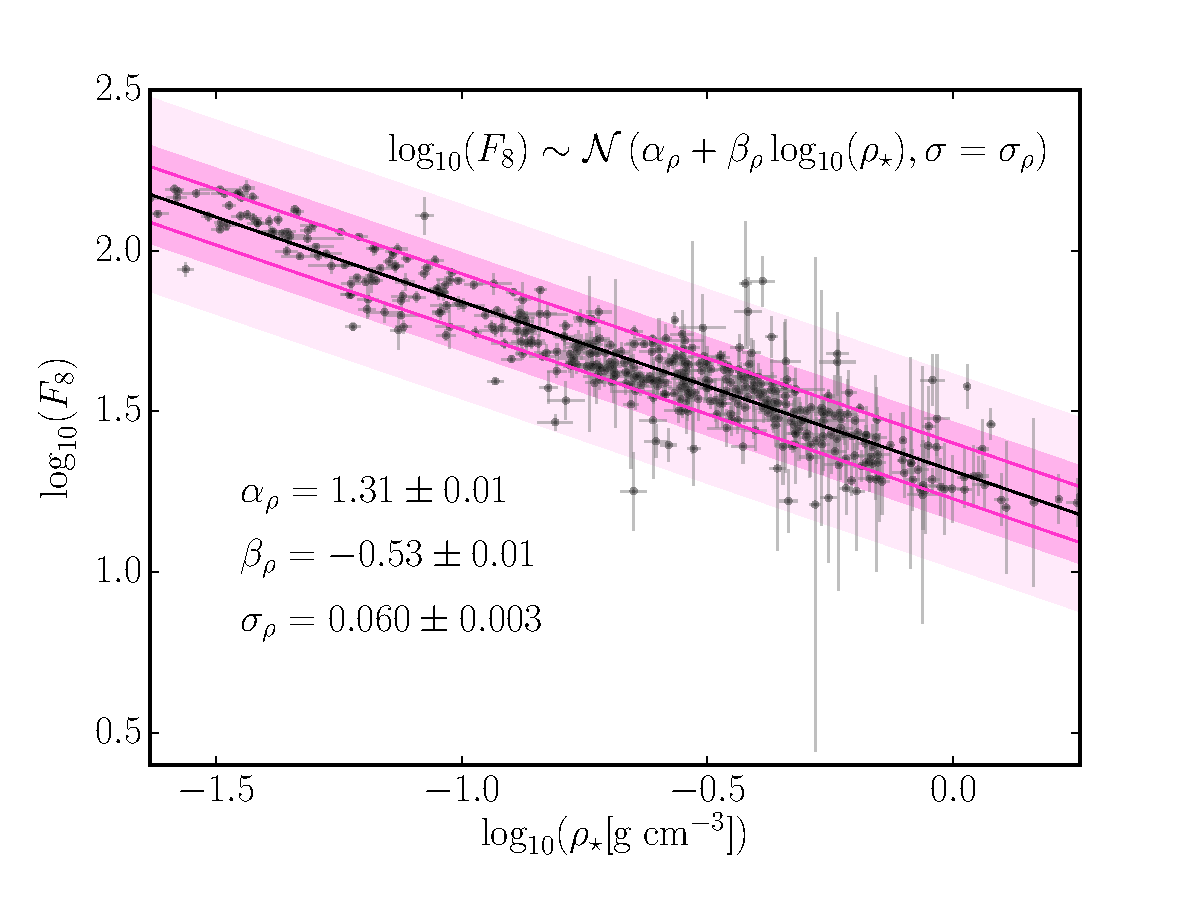
\includegraphics[width=8.4cm,angle=0,clip=true]{figures/flicker_vs_rho.pdf}
% \includegraphics[width=8.4cm,angle=0,clip=true]{../figs/rho_vs_flicker.pdf}
% \includegraphics[width=8.4cm,angle=0,clip=true]{new_rho.pdf}
\caption{
Stellar density vs. flicker.
This figure shows the model, conditioned on the data.
The solid black line shows the model with the best-fitting parameter values
quoted in the text.
The solid pink lines show the 1$\sigma$ region where the extra scatter is not
included and the pink shaded regions show the 1 and 2$\sigma$ regions with the
additional scatter.}
\label{fig:rhostar}
\end{center}
\end{figure}

%%% logg plot
\begin{figure}
\begin{center}
\includegraphics[width=8.4cm,angle=0,clip=true]{figures/flicker_vs_logg.pdf}
% \includegraphics[width=8.4cm,angle=0,clip=true]{../figs/logg_vs_flicker.pdf}
% \includegraphics[width=8.4cm,angle=0,clip=true]{new_logg.pdf}
\caption{
$\log(g)$ vs. flicker.
As in \ref{fig:rhostar} this figure shows the model, conditioned on the data.
The solid black line shows the model with the best-fitting parameter values
quoted in the text.
The solid blue lines show the 1$\sigma$ region where the extra scatter is not
included and the blue shaded regions show the 1 and 2$\sigma$ regions with the
additional scatter.}
\label{fig:logg}
\end{center}
\end{figure}

\begin{table}
\begin{center}
\caption{Median parameter values with 1$\sigma$ uncertainties.}
\begin{tabular}{lcc}
\hline\hline
Parameter & Median value \\
    \hline
$\alpha_\rho$   &    1.315$\pm 0.008$   \\
$\beta_\rho$    &    -0.526$\pm 0.009$   \\
$\sigma_\rho$   &    0.065$\pm 0.003$   \\
% 1.31476104613 0.00759733599155 0.00767814819025
% -0.525867117083 0.00913323668806 0.00926420817321
% 0.0650160215492 0.00300880167448 0.00288553857806
\hline
$\alpha_g$      &    4.90$\pm 0.05$   \\
$\beta_g$       &   -0.83$\pm 0.01$   \\
$\sigma_g$      &    0.056$\pm 0.003$   \\
% 4.90451472909 0.0514398889837 0.0509386027456
% -0.8252952869 0.0130730719222 0.0131097233196
% 0.0565263079576 0.00279179051697 0.00271277097572
    \hline
\end{tabular}
\end{center}
\end{table}
\label{tab:results}

\section{DISCUSSION}
\label{sec:discussion}

%% DISCUSSION
%%

We have recalibrated the relation between short timescale brightness
fluctuations in the {\it Kepler} light curves of stars (flicker) with both
stellar density and surface gravity, whilst including parameters to describe
the intrinsic scatter in these relationships, presented in table
\ref{tab:results}.
The additive terms, $\sigma_\rho$ and $ \sigma_g$ are both non-zero,
suggesting that there {\it is} an additional source of scatter in the
relations, not accounted for by the observational uncertainties alone.
This is either caused by intrinsic scatter in the physical relationship
between flicker and density and \logg, produced by some physical process that
is not accounted for in the model, or by an underestimation of the
observational uncertainties.
We also tested a model with both an additive variance term {\it and} a term
that included flicker-dependent variance.
We found that the need for additional flicker-dependent variance was not
supported by the data, indicating that the intrinsic scatter in the relations
between flicker, \logg\ and \rhostar\ does not depend on evolutionary state.

This is a simple `fitting a line to data' exercise, however it continues the
discussion of probabilistic modelling that is an active topic within the
fields of exoplanet and stellar astronomy.
We used Hierarchical Bayesian Modelling (HBM) to constrain the intrinsic
scatter in the relationship between flicker, surface gravity and density and
included the effects of the non-negligable two-dimensional observational
uncertainties.
% Although none of these methods, nor the data used here are new taken alone,
% we use the example of flicker to demonstrate the ideas and the importance of
% probabilistic, hierarchical inference.
Relationships between astronomical parameters are almost always
non-deterministic; an element of stochasticity effects the physical parameters
of stars so one can never perfectly predict $y$ given an observation of $x$.
We advocate a probabilistic approach in both the `fitting the model to data'
step, {\it and} when using an empirically calibrated model to predict
parameter values.
The fitting stage benefits because if the relationships between parameters are
falsely assumed to be deterministic, they will be skewed by data points with
uncertainties that only represent measurement error and no additional scatter.
The prediction stage benefits from the stochastic treatment both because a
probability distribution is in many ways more representative of an observation
than a point estimate, and because posterior PDF samples can be used in
subsequent studies (provided the prior used during the fitting process is
described).

We provide posterior PDF samples and the code used in this project at
\url{https://zenodo.org/deposit/95681/}.
% https://github.com/RuthAngus/flicker
Whenever a prediction for the surface gravity or density of a star is required,
for a given estimate of flicker, we recommend using these posterior samples
within the calculation of \rhostar or \logg\ and its (Monte Carlo)
uncertainty.
These posterior samples will naturally fold in the covariances between
parameters.
Simple analytical uncertainty propagation is only valid when uncertainties are
Gaussian and uncorrelated which is rarely true and certainly not the case when
the model is a straight line (the slope and intercept are alway correlated).
A flicker value with uncertainties (or even better: posterior PDF
samples), input into our model will result in a probability distribution over
stellar densities or surface gravities which reflects both the uncertainties
on the flicker measurement, the uncertainties on the model parameters {\it and}
the intrinsic scatter in the flicker-\rhostar-\logg\ relations.


% #####################################################################
% %% Bibliography
% \begin{thebibliography}{99}
% \bibitem[\protect\citeauthoryear{Andrieu \& Roberts}{2009}]{andrieu:2009}
% Andrieu, C., \& Roberts, G.~O., Ann. Statist., 2, 695
% \bibitem[\protect\citeauthoryear{Angus et al.}{2015}]{angus:2015}
% Angusr, R., Aigrain, S., Foreman-Mackey, D. \& McQuillan, A., 2015, MNRAS,
% 450, 1787
% \bibitem[\protect\citeauthoryear{Bastien et al.}{2013}]{bastien:2013} Bastien,
% F. A., Stassun, K. G., Basri, G. \& Pepper, J., 2013, Nature, 500, 427
% \bibitem[\protect\citeauthoryear{Chaplin et al.}{2014}]{chaplin:2014}
% Chaplin, W.~J., Basu, S., Huber, D. et al., 2014, ApJS, 210, 1
% \bibitem[\protect\citeauthoryear{Cranmer et al.}{2014}]{cranmer:2014}
% Cranmer, S. R., Bastien, F. A., Stassun, K. G. \& Saar, S. H., 2014, ApJ, 781,
% 124
% \bibitem[\protect\citeauthoryear{Foreman-Mackey et al.}{2014}]
% {foreman-mackey:2014} Foreman-Mackey, D., Hogg, D.~W. \& Morton, T.~D., 2014,
% ApJ, 795, 64
% \bibitem[Foreman-Mackey et al.(2013)]{foreman-mackey:2013}
% Foreman-Mackey, D., Hogg, D.~W., Lang, D., \& Goodman, J.\ 2013, \pasp, 125, 306
% \bibitem[\protect\citeauthoryear{Fox}{1997}]{fox:1997}
% Fox, J., 1997, Applied Regression Analysis, Linear Models, and Related Methods
% (Thousand Oaks:Sage Publications, Inc.)
% \bibitem[\protect\citeauthoryear{Fuller}{1987}]{fuller:1987}
% Fuller, W.~A., 1987, Wiley Series in Probability and Mathematical Statistics
% \bibitem[\protect\citeauthoryear{Hogg et al.}{2010}]{hogg:2010}
% Hogg, D.~W., Myers, A.~D. \& Bovy, J., 2010, ApJ, 725,
% 2166
% \bibitem[\protect\citeauthoryear{Hogg et al.}{2010b}]{hogg:2010b}
% Hogg, D.~W., Bovy, J. \& Lang, D., 2010
% \bibitem[\protect\citeauthoryear{Huber et al.}{2013}]{huber:2013}
% Huber, D., Chaplin, W.~J., Christensen-Dalsgaard, J. et al., 2013, ApJ, 767,
% 127
% \bibitem[\protect\citeauthoryear{Kelly}{2007}]{kelly:2007} Kelly, B.~C., 2007,
% ApJ, 665, 1489
% \bibitem[\protect\citeauthoryear{Kipping et al.}{2014}]{kipping:2014}
% Kipping, D.~M., Bastien, F.~A., Stassun, K.~G., Chaplin, W.~J., Huber, D. \&
% Buchhave, L.~A., 2014, ApJ, 785, 32
% \bibitem[\protect\citeauthoryear{Rogers}{2015}]{rogers:2015}
% Rogers, L.~A., 2015, ApJ, 801, 41
% \bibitem[\protect\citeauthoryear{Seager \& Mall\'{e}n-Ornelas}{2003}]
% {seager:2003}Seager, S., \& Mall\'{e}n-Ornelas, G., 2003, ApJ, 585, 1038
% \bibitem[VanderPlas(2014)]{vanderplas}
% VanderPlas, J.\ 2014, arXiv:1411.5018
% \bibitem[\protect\citeauthoryear{Wolfgang et al.}{2015}]{wolfgang:2015}
% Wolfgang, A., Rogers, L.~A., Ford, E.~B., 2015, ApJ, submitted
% (astro-ph:1504.07557)
% \end{thebibliography}

\chapter{Future work}

\section{Future instruments}

\subsection{\Ktwo}

\subsection{\TESS}

\subsection{\LSST}

The Large Synoptic Survey Satellite (LSST) is a 8.4 metre telescope with a 9.6
square degree field of view in Cerro Pach\'{o}n, Chile, currently under
construction.
It is designed to observe 18,000 square degrees in the southern sky (south of
+10 degrees, declination) in six Sloan Digital Sky Survey (\SDSS) filters:
ugrizy.
During its main mode of operation (90\% of the time), \LSST\ will perform two
fifteen second exposures per visit, with one thousand visits per night and
will have a faint limit of around 24.5 in r-band.
For the remaining 10\% of the time, \LSST\ will focus on a small number of
`deep drilling fields'.
These fields are yet to be determined but could be, for example, the Large and
Small Magellanic Clouds, the galactic plane, and so on.
These fields will receive targeted, repeat observations of, for instance 200
observations over a 40-hour period after which the faint limit could be
extended to around 28 apparent magnitudes (CITE THE WEBSITE?).
This faint limit will be extended for fields with co-added exposures.
First light is currently scheduled for 2021.
Data release one of eleven is expected to contain eighteen billion objects.

\LSST\ will provide rotation periods for a new stellar regime.
Because \kepler\ targeted Earth-like planet hosts, the majority of its
targets were G stars, with fewer K and M dwarfs.
Since the collecting area of \LSST\ is so large it will be sensitive to a
large number of faint stars, including many K and M dwarfs.
Since it is not a space mission and its lifetime does not depend on the
reliability of moving parts or fuel, \LSST\ will run for 10 years---more than
double the length of the \kepler prime mission.
This will open up an opportunity to detect rotation signatures in faint,
slowly rotating stars, allowing us to populate both the low-mass and old parts
of the age-rotation parameter space.
In many ways \LSST\ is \kepler's antithesis: \kepler data is dense and evenly
spaced, whereas \LSST\ light curves will have sparse, irregular cadence.
Depending on its location on the sky, a given target will have between ... and
... data points spread over 10 years, spaced from 3 days to 30 days apart.
The disadvantage of this is that there will be a rotation period lower limit.
The advantage of using sparse data however, is that CPU time is vastly
reduced!

We simulated \LSST cadence by requiring that an object/field only be observed
during the night and whilst the field is visible, so for half of the year.
Each object is visited every three days, on average during the observable
season and visits are clustered around a season with a Gaussian shape.
A histogram of the number of visits per week as a function of time for a given
object or field is shown in figure \ref{fig:cadence_hist}.

\begin{figure}
\begin{center}
\includegraphics[width=6in, clip=true]{figures/cadence_hist}
\caption[An LSST cadence histogram.]
{A histogram of the number of visits per week as a function of time
for a given object or field observed by \LSST as used in our simulations.}
\label{fig:cadence_hist}
\end{center}
\end{figure}

Since \LSST observations are not evenly spaced, it is not trivial to compute
an autocorrelation function.
(LOOK UP COLLIER-CAMERON AND MAZEH)
One could interpolate the light curve onto an evenly spaced grid and then
compute the ACF, but this would introduce a large amount of uncertainty.
Instead of using an ACF to initialise our MCMC we therefore use the
Lomb-Scargle periodogram.

\subsection{\PLATO}

\section{Future projects}

information, so these will be used too) and will be tested on binary stars.
In addition to the basic input catalogues available for the transit survey
stars, I will gather information from every other available source.
Light curves themselves are rich in age information, for example, even where
a rotation period cannot be measured, the {\it absence} of discernable
variability is indicative of old-age.
I will use the method of \citet{bastien} to measure short-timescale brightness
fluctuations (known as flicker) which are correlated with surface gravity.
I will also use new distance and proper motion information from GAIA as soon as
the data become available (expected in early 2017).
To obtain accurate gyrochronological ages, reliable rotation periods must be
inferred---this is another challenge which has prohibited the exploration of
time-dependent exoplanet populations thus far.
Standard methods for rotation period inference such as autocorrelation
functions (ACFs) and sine-fitting periodograms are not optimal for noisy light
curves with low-amplitude signals, are not probabilistic, do not provide
realistic uncertainties and are performed on `detrended' \Kepler\ light curves
with significantly reduced power at periods of 30 days and above.
My new technique for measuring probabilistic rotation periods using Gaussian
processes (GPs) can extract rotation periods from low-amplitude signals that
are buried in noisy data, can be applied directly to unprocessed light curves
and measures more precise and accuration rotation periods than ACF and
periodogram methods \citep{AngusIAU}, see figure \ref{fig:rotation}.
I will use this method to compute a probabilistic constraint on the rotation
periods of {\it all} transit survey stars.

This new dating method will be probabilistic---hierarchical Bayesian inference
will be performed in order to `learn' an informative age prior from the data
themselves; a prior that will reflect the most probable age of a star, given
the age distribution of other stars observed.

There are several advantages to this dating model.
Firstly, combining all the information will provide more precise and accurate
ages than any one method used on its own, and, by definition, these ages will
be less dependent upon one single model.
Secondly, it will provide an age constraint for every star observed by
a photometric survey since {\it some} age information is always available.
Thirdly, it will be directly compatible with my probabilistic, GP rotation
period measurement method and finally, it will be easily updated as new data
become available.
By modelling stellar ages using all available information and combining
multiple dating techniques, my hierarchical, Bayesian dating method with
informative priors {\bf will provide the most precise and accurate ages ever
inferred for every star observed by \Kepler, \Ktwo\ and \TESS}.

This project is highly ambitious and will have enormous impact if successful,
however even if there is no detectable age-trend in the \Kepler\ data it will
lead to other discoveries and useful products for the astronomical
community.
Firstly, a rotation period and age for every \Kepler, \Ktwo\ and \TESS\ star
will be beneficial to both exoplaneteers and galactic archaeologists alike,
\citep[e.g.][]{bovy}.
Secondly, stellar rotation periods can reveal potential star-planet
interactions in which a planet transfers angular momentum to its host---I
intend to unambiguously confirm this phenomenon.
Finally, this work will pave the way for exoplanet-age studies with PLATO.
Launching in 2025, this space telescope will provide highly precise
asteroseismic ages for thousands of stars, revolutionising the field of
stellar ages.


\chapter{Conclusions}
\label{chapter:conclusions}

In chapter \ref{chapter:gyro} I used new results from \kepler\
asteroseismology to recalibrate the relation between rotation period, age and
colour.
The light curves of several cool dwarf, Solar-like oscillators were analysed
by \citet{Chaplin2014} who provide a catalogue of ages for these targets via
the methods described in \textsection \ref{section:asteroseismology} of
chapter \ref{chapter:intro}.
We used rotation periods of these stars from \citet{Garcia2014} who measure
the periodicity of signals in \kepler\ light curves using the ACF and wavelet
methods described in \textsection \ref{rotation}.
We fit a gyrochronology model to these data, of the form
\begin{equation}
P = A^n \times a(B-V-c)^b,
\end{equation}
\label{eq:Barnes2007_2}
where $P$ is rotation period (in days),
$A$ is age (in Myr), $B$ and $V$ are B and V band magnitudes respectively and
$a$, $b$, $c$ and $n$ are dimensionless free parameters.
We found evidence to suggest that this function does not provide a good fit to
the data and that some old \kepler\ asteroseismic targets are more rapidly
rotating that expected, given their age and colour.
\citet{Vansaders2016} present an adaptation to their theoretical model which
{\it is} able to reproduce the trends in this data set.
They suggest that there is a critical Rossby number ($Ro=2.16$) at which the
magnetic dynamo that drives angular momentum loss shuts off.
New rotation periods from the repurposed \kepler\ mission, \ktwo\ may shed
light on this controversial topic.

In chapter \ref{chapter:sip} I present a method for searching for periodic
signals (\eg rotation periods) without detrending.
The pointing precision of \kepler\ was dramatically reduced when its third
reaction wheel broke.
\ktwo\ light curves are contaminated with high amplitude systematic features
as a result.
Detrending these light curves is essential in order to search for exoplanets
or measure stellar rotation periods.
Instead of detrending, we model the noise and the signal simultaneously and
marginalise over the noise model.
A noise model is constructed by decomposing all \ktwo\ light curves from
campaign 1 into a set of orthogonal basis vectors called `Eigen Light Curves'
(ELCs).
The Systematics-Insensitive Periodogram (SIP) uses a linear combination of
150 of these ELCs to model a light curve while simulataneously fitting a
sinusoid to the data at a given frequency.
Finding the amplitudes of the best-fit sinusoids over a grid of frequencies
produces a SIP.
The SIP is particularly effective for red giant asteroseismology as these
signals are typically sinusoidal and plagued by a six-hour thruster firing
signal that most detrending algorithms are unable to remove.
The capabilities of the SIP are limited for rotation period inference as
it is difficult to separate systematics from physical signals on long
timescales and because a sinusoid is an imperfect model for stellar rotation.

In chapter \ref{chapter:GP} I present a new method for inferring precise and
accurate rotation periods from \kepler\ light curves using Gaussian processes.
I compare the GP method to the Lomb-Scargle periodogram and ACF methods,
finding it to be more accurate and precise than both.
In addition it provides accurate uncertainties because full a posterior PDF of
the rotation period parameter is explored.
Unfortunately, while this method works well on noise-free simulations, it is
currently extremely computationally expensive when applied to noisy light
curves.
It is therefore currently most useful for individual targets rather than large
ensembles of light curves.

In the final chapter of this thesis I use \kepler\ flicker estimates and
asteroseismology data to recalibrate the relation between flicker, surface
gravity and stellar density.
These relations are not deterministic, although they have been treated as such
in the past and there is significant intrinsic scatter that is not accounted
for by the observational uncertainties.
I use hierarchical probabilistic modelling to quantify  model these relations
and quantify the additional scatter.

I began this thesis by introducing the \kepler\ spacecraft which has provided
all the data used in this work.
I would like to conclude by saying that, in my opinion, \kepler's legacy has
to be the greatest of any astronomical instrument ever built.
Not just for exoplanets but for stellar astrophysics too.
\kepler\ has revived the astronomical communities general interest in stars:
after all, one can only understand an exoplanet as well as one understands the
star that it orbits.
Were it not for \kepler, this thesis would look very different and I, for one,
am grateful for the unique challenges posed by its rich, unrivalled data set.

%% This defines the bibliography file (main.bib) and the bibliography style.
%% If you want to create a bibliography file by hand, change the contents of
%% this file to a `thebibliography' environment.  For more information 
%% see section 4.3 of the LaTeX manual.
\begin{singlespace}
\bibliography{main}
\bibliographystyle{plain}
\end{singlespace}

\end{document}
